% Options for packages loaded elsewhere
\PassOptionsToPackage{unicode}{hyperref}
\PassOptionsToPackage{hyphens}{url}
%
\documentclass[
  12pt,
  man,floatsintext]{apa7}
\usepackage{amsmath,amssymb}
\usepackage{lmodern}
\usepackage{setspace}
\usepackage{iftex}
\ifPDFTeX
  \usepackage[T1]{fontenc}
  \usepackage[utf8]{inputenc}
  \usepackage{textcomp} % provide euro and other symbols
\else % if luatex or xetex
  \usepackage{unicode-math}
  \defaultfontfeatures{Scale=MatchLowercase}
  \defaultfontfeatures[\rmfamily]{Ligatures=TeX,Scale=1}
\fi
% Use upquote if available, for straight quotes in verbatim environments
\IfFileExists{upquote.sty}{\usepackage{upquote}}{}
\IfFileExists{microtype.sty}{% use microtype if available
  \usepackage[]{microtype}
  \UseMicrotypeSet[protrusion]{basicmath} % disable protrusion for tt fonts
}{}
\makeatletter
\@ifundefined{KOMAClassName}{% if non-KOMA class
  \IfFileExists{parskip.sty}{%
    \usepackage{parskip}
  }{% else
    \setlength{\parindent}{0pt}
    \setlength{\parskip}{6pt plus 2pt minus 1pt}}
}{% if KOMA class
  \KOMAoptions{parskip=half}}
\makeatother
\usepackage{xcolor}
\usepackage{graphicx}
\makeatletter
\def\maxwidth{\ifdim\Gin@nat@width>\linewidth\linewidth\else\Gin@nat@width\fi}
\def\maxheight{\ifdim\Gin@nat@height>\textheight\textheight\else\Gin@nat@height\fi}
\makeatother
% Scale images if necessary, so that they will not overflow the page
% margins by default, and it is still possible to overwrite the defaults
% using explicit options in \includegraphics[width, height, ...]{}
\setkeys{Gin}{width=\maxwidth,height=\maxheight,keepaspectratio}
% Set default figure placement to htbp
\makeatletter
\def\fps@figure{htbp}
\makeatother
\setlength{\emergencystretch}{3em} % prevent overfull lines
\providecommand{\tightlist}{%
  \setlength{\itemsep}{0pt}\setlength{\parskip}{0pt}}
\setcounter{secnumdepth}{-\maxdimen} % remove section numbering
% Make \paragraph and \subparagraph free-standing
\ifx\paragraph\undefined\else
  \let\oldparagraph\paragraph
  \renewcommand{\paragraph}[1]{\oldparagraph{#1}\mbox{}}
\fi
\ifx\subparagraph\undefined\else
  \let\oldsubparagraph\subparagraph
  \renewcommand{\subparagraph}[1]{\oldsubparagraph{#1}\mbox{}}
\fi
\newlength{\cslhangindent}
\setlength{\cslhangindent}{1.5em}
\newlength{\csllabelwidth}
\setlength{\csllabelwidth}{3em}
\newlength{\cslentryspacingunit} % times entry-spacing
\setlength{\cslentryspacingunit}{\parskip}
\newenvironment{CSLReferences}[2] % #1 hanging-ident, #2 entry spacing
 {% don't indent paragraphs
  \setlength{\parindent}{0pt}
  % turn on hanging indent if param 1 is 1
  \ifodd #1
  \let\oldpar\par
  \def\par{\hangindent=\cslhangindent\oldpar}
  \fi
  % set entry spacing
  \setlength{\parskip}{#2\cslentryspacingunit}
 }%
 {}
\usepackage{calc}
\newcommand{\CSLBlock}[1]{#1\hfill\break}
\newcommand{\CSLLeftMargin}[1]{\parbox[t]{\csllabelwidth}{#1}}
\newcommand{\CSLRightInline}[1]{\parbox[t]{\linewidth - \csllabelwidth}{#1}\break}
\newcommand{\CSLIndent}[1]{\hspace{\cslhangindent}#1}
\ifLuaTeX
\usepackage[bidi=basic]{babel}
\else
\usepackage[bidi=default]{babel}
\fi
\babelprovide[main,import]{english}
% get rid of language-specific shorthands (see #6817):
\let\LanguageShortHands\languageshorthands
\def\languageshorthands#1{}
% Manuscript styling
\usepackage{upgreek}
\captionsetup{font=singlespacing,justification=justified}

% Table formatting
\usepackage{longtable}
\usepackage{lscape}
% \usepackage[counterclockwise]{rotating}   % Landscape page setup for large tables
\usepackage{multirow}		% Table styling
\usepackage{tabularx}		% Control Column width
\usepackage[flushleft]{threeparttable}	% Allows for three part tables with a specified notes section
\usepackage{threeparttablex}            % Lets threeparttable work with longtable

% Create new environments so endfloat can handle them
% \newenvironment{ltable}
%   {\begin{landscape}\centering\begin{threeparttable}}
%   {\end{threeparttable}\end{landscape}}
\newenvironment{lltable}{\begin{landscape}\centering\begin{ThreePartTable}}{\end{ThreePartTable}\end{landscape}}

% Enables adjusting longtable caption width to table width
% Solution found at http://golatex.de/longtable-mit-caption-so-breit-wie-die-tabelle-t15767.html
\makeatletter
\newcommand\LastLTentrywidth{1em}
\newlength\longtablewidth
\setlength{\longtablewidth}{1in}
\newcommand{\getlongtablewidth}{\begingroup \ifcsname LT@\roman{LT@tables}\endcsname \global\longtablewidth=0pt \renewcommand{\LT@entry}[2]{\global\advance\longtablewidth by ##2\relax\gdef\LastLTentrywidth{##2}}\@nameuse{LT@\roman{LT@tables}} \fi \endgroup}

% \setlength{\parindent}{0.5in}
% \setlength{\parskip}{0pt plus 0pt minus 0pt}

% Overwrite redefinition of paragraph and subparagraph by the default LaTeX template
% See https://github.com/crsh/papaja/issues/292
\makeatletter
\renewcommand{\paragraph}{\@startsection{paragraph}{4}{\parindent}%
  {0\baselineskip \@plus 0.2ex \@minus 0.2ex}%
  {-1em}%
  {\normalfont\normalsize\bfseries\itshape\typesectitle}}

\renewcommand{\subparagraph}[1]{\@startsection{subparagraph}{5}{1em}%
  {0\baselineskip \@plus 0.2ex \@minus 0.2ex}%
  {-\z@\relax}%
  {\normalfont\normalsize\itshape\hspace{\parindent}{#1}\textit{\addperi}}{\relax}}
\makeatother

% \usepackage{etoolbox}
\makeatletter
\patchcmd{\HyOrg@maketitle}
  {\section{\normalfont\normalsize\abstractname}}
  {\section*{\normalfont\normalsize\abstractname}}
  {}{\typeout{Failed to patch abstract.}}
\patchcmd{\HyOrg@maketitle}
  {\section{\protect\normalfont{\@title}}}
  {\section*{\protect\normalfont{\@title}}}
  {}{\typeout{Failed to patch title.}}
\makeatother

\usepackage{xpatch}
\makeatletter
\xapptocmd\appendix
  {\xapptocmd\section
    {\addcontentsline{toc}{section}{\appendixname\ifoneappendix\else~\theappendix\fi\\: #1}}
    {}{\InnerPatchFailed}%
  }
{}{\PatchFailed}
\keywords{conceptual processing, semantic priming, semantic decision, lexical decision, language, vision, vocabulary size, statistical power}
\usepackage{csquotes}
\renewcommand\author[1]{}
\renewcommand\affiliation[1]{}
\authorsnames[1, 2, 2]{Pablo Bernabeu, Dermot Lynott, Louise Connell}
\authorsaffiliations{{Department of Psychology, Lancaster University, UK}, {Department of Psychology, Maynooth University, Ireland}}
\renewcommand{\topfraction}{.75}
\renewcommand{\bottomfraction}{.4}
\renewcommand{\textfraction}{.15}
\renewcommand{\floatpagefraction}{.6}
\setlength{\@fptop}{0pt}
\setcounter{topnumber}{3}
\setcounter{bottomnumber}{2}
\setcounter{totalnumber}{4}
\usepackage{placeins}
\usepackage{amsmath}
\usepackage{upgreek}
\usepackage{booktabs}
\usepackage{longtable}
\usepackage{array}
\usepackage{multirow}
\usepackage{wrapfig}
\usepackage{float}
\usepackage{colortbl}
\usepackage{pdflscape}
\usepackage{tabu}
\usepackage{threeparttable}
\usepackage{threeparttablex}
\usepackage[normalem]{ulem}
\usepackage{makecell}
\usepackage{xcolor}
\renewcommand\appendix{}
\ifLuaTeX
  \usepackage{selnolig}  % disable illegal ligatures
\fi
\IfFileExists{bookmark.sty}{\usepackage{bookmark}}{\usepackage{hyperref}}
\IfFileExists{xurl.sty}{\usepackage{xurl}}{} % add URL line breaks if available
\urlstyle{same} % disable monospaced font for URLs
\hypersetup{
  pdftitle={Language and vision in conceptual processing: Multilevel analysis and statistical power},
  pdflang={en-EN},
  pdfkeywords={conceptual processing, semantic priming, semantic decision, lexical decision, language, vision, vocabulary size, statistical power},
  hidelinks,
  pdfcreator={LaTeX via pandoc}}

\title{Language and vision in conceptual processing: Multilevel analysis and statistical power}
\author{\phantom{0}}
\date{}


\shorttitle{LANGUAGE AND VISION IN CONCEPTUAL PROCESSING}

\authornote{

\addORCIDlink{Pablo Bernabeu}{0000-0003-1083-2460}

\addORCIDlink{Dermot Lynott}{0000-0001-7338-0567}

\addORCIDlink{Louise Connell}{0000-0002-5291-5267}

This manuscript is a draft. Correspondence can be addressed to Pablo Bernabeu on \href{mailto:pcbernabeu@gmail.com}{\nolinkurl{pcbernabeu@gmail.com}}. All the materials needed to inspect and reproduce the present research---comprising documentation, data, analysis and results---are available at \url{http://doi.org/10.17605/OSF.IO/UERYQ}.

}

\affiliation{\phantom{0}}

\abstract{%
Research has suggested that conceptual processing depends on both language-based and vision-based information. We tested this interplay at three levels of the experimental structure: individuals, words and tasks. To this end, we drew on three existing, large data sets that implemented the paradigms of semantic priming, semantic decision and lexical decision. We extended these data sets with measures of language-based and vision-based information, and analysed how the latter variables interacted with participants' vocabulary size and gender, and also with presentation speed in the semantic priming study. We performed the analysis using mixed-effects models that included a comprehensive array of fixed effects---including covariates---and random effects. First, we found that language-based information was found to be more important than vision-based information. Second, in the semantic priming study---whose task required distinguishing between words and nonwords---, both language-based and vision-based information were more influential when words were presented faster. Third, a `task-relevance advantage' was identified in higher-vocabulary participants. Specifically, in lexical decision, higher-vocabulary participants were more sensitive to language-based information than lower-vocabulary participants. In contrast, in semantic decision, higher-vocabulary participants were more sensitive to word concreteness. Fourth, we demonstrated the influence of the analytical method on the results. These findings support the interplay between language and vision in conceptual processing, and demonstrate the influence of measurement instruments on the results. Last, we estimated the sample size required to reliably investigate various effects. We found that 300 participants were sufficient to examine the effect of language-based information contained in words, whereas more than 1,000 participants were necessary for the effect of vision-based information and for the interactions of both former variables with vocabulary size, gender and presentation speed. In conclusion, this power analysis reveals the need to increase sample sizes for research on perceptual simulation and individual differences.
}



\begin{document}
\maketitle

\setstretch{1.5}
\hypertarget{section}{%
\section{}\label{section}}

Over the last two decades, research in the cognitive sciences has suggested that conceptual processing depends on both language and embodiment systems. That is, understanding words involves---on the one hand---lexical and semantic associations of an amodal kind, and---on the other hand---modality-specific associations within perceptual, motor, affective and social domains (Barsalou et al., 2008; Connell, 2019; Davis \& Yee, 2021; Khatin-Zadeh et al., 2021; Vigliocco et al., 2009). Studies addressing these systems have found that the language system is overall more prevalent in word processing, producing larger effect sizes (Banks et al., 2021; Kiela \& Bottou, 2014; Lam et al., 2015; Louwerse et al., 2015; Pecher et al., 1998; Petilli et al., 2021). More intricately, the roles of language and embodiment are modulated by the characteristics of individuals, words and tasks. For instance, people's individual experience with language is associated with differential effects relating to phonological, lexical and semantic features of words (Jared \& O'Donnell, 2017; Pexman \& Yap, 2018; Yap et al., 2009, 2012, 2017). Similarly, physical expertise and perceptual biases are associated with differences in the mental simulation of meaning (Beilock et al., 2008; Calvo-Merino et al., 2005; Vukovic \& Williams, 2015). Furthermore, the embodiment system is especially suited for the processing of concrete concepts---e.g., \emph{red}, \emph{building} (C. R. Jones et al., 2022; Kousta et al., 2011; Ponari, Norbury, Rotaru, et al., 2018; cf. Borghi et al., 2022). Embodied information also becomes more important in the following conditions: (I) later in the time courses of word recognition (Bernabeu et al., 2017; Louwerse \& Hutchinson, 2012; cf. Petilli et al., 2021) and property generation (Santos et al., 2011; Simmons et al., 2008), (II) when participants produce slower responses (Louwerse \& Connell, 2011), and (III) in tasks that elicit deeper semantic processing---e.g., semantic decision, as opposed to lexical decision (Ostarek \& Huettig, 2017; Petilli et al., 2021). Last, research in computational linguistics has provided further support for the complementarity of language and embodied information, by revealing increased predictive performance when models are provided with perceptual information on top of text-based information (Frome et al., 2013; Roads \& Love, 2020).

In spite of the amount of evidence demonstrating the interplay between language and embodiment, there are four reasons to continue testing the interplay theory. First, the coexistence of several systems in a scientific theory must be thoroughly justified due to the value of simplicity (Gallese \& Lakoff, 2005; Tillman et al., 2015). This scrutiny is particularly necessary because the language system has consistently produced larger effect sizes than the embodiment system (Banks et al., 2021; Kiela \& Bottou, 2014; Lam et al., 2015; Louwerse et al., 2015; Pecher et al., 1998; Petilli et al., 2021). Therefore, it should be ruled out that the language system can suffice in all contexts.

Second, it is important to examine both language and embodiment across various levels of the experimental structure---namely, individuals (i.e., due to individual differences such as vocabulary size), words (i.e., lexical and semantic variables) and tasks (i.e., experimental conditions affecting, for instance, processing speed). Some studies have approached this comprehensive structure but there is still room to widen the scope. One of the findings revealed by cross-level analyses is the influence of word processing tasks on the importance of modality-specific information. For instance, Connell and Lynott (2014) found that the vision-based information in words is important both for word identification (i.e., lexical decision) and for reading aloud (i.e., naming). In contrast, the auditory information in words is important for reading aloud but not so much for word identification. Another finding from cross-level research is a `task-relevance advantage' for individuals that have a greater linguistic experience. Specifically, Pexman and Yap (2018) found that higher-vocabulary individuals were more sensitive to task-relevant information, such as word concreteness in the semantic decision task. Furthermore, regarding embodiment, research has revealed that individuals who are briefly exposed to a certain sport develop neural activity that allows them to mentally simulate sport-specific actions during language processing (Beilock et al., 2008). While these works have covered a large swathe of the present topic, one question remains unanswered: how does an individual's linguistic experience relate to their sensivity to both linguistic and embodied information in words?

Third, there is some inconclusive evidence. First, some findings have suggested that higher-vocabulary participants are more sensitive to language-based information---as reflected in greater semantic priming (Yap et al., 2017)---, whereas other findings have suggested the opposite (Yap et al., 2009). Second, some studies have suggested that the language system is activated before the embodiment system (Lam et al., 2015; Louwerse \& Connell, 2011), whereas a recent study suggested that this pattern does not hold in the lexical decision task (Petilli et al., 2021). Third, some evidence has suggested that female participants draw on the language system more prominently than males (Burman et al., 2008; Hutchinson \& Louwerse, 2013; Jung et al., 2019; Ullman et al., 2008), whereas other research has suggested that this difference is negligible in the general population (Wallentin, 2020).

Fourth, some of the previous studies could have been affected by the scarcity of statistical power that has been identified in cognitive psychology and neuroscience (Lynott et al., 2014; Marek et al., 2022; Montero-Melis et al., 2022). Problematically, low-powered studies present more errors in the estimation of effect sizes and \(p\) values (Heyman et al., 2018; Loken \& Gelman, 2017; Vasishth, Mertzen, et al., 2018). The current studies address these four key issues.

\hypertarget{present-studies}{%
\section{The present studies}\label{present-studies}}

We revisit three larger-than-average studies to investigate the interplay between language and embodiment in conceptual processing. We devote a study to each of the three original studies. Thus, Study 1 is centred on Hutchison et al. (2013) and uses the semantic priming paradigm. Study 2 is centred on Pexman et al. (2017) and uses the semantic decision paradigm. Study 3 is centred on Balota et al. (2007) and uses the lexical decision paradigm. Each of these central studies contained measures of participants' vocabulary size and gender. Furthermore, the core data sets were expanded by adding variables that captured the language-based information in words (Mandera et al., 2017; Wingfield \& Connell, 2022a) and the vision-based information in words (Lynott et al., 2020; Petilli et al., 2021)---the latter being used to represent the embodiment system. One of the key questions we investigated using this array of variables was whether individual differences in vocabulary and gender modulated participants' sensivity to the language-based and vision-based information in words. Alongside the effects of interest, several covariates were included in the models to allow a rigorous analysis (Sassenhagen \& Alday, 2016). These covariates comprised measures of general cognition and lexical characteristics of the stimulus words. Last, in each study, we performed a statistical power analysis to help estimate the sample size needed to investigate a variety of effects in future studies.

Below, we delve into the language and the embodiment components of these studies.

\hypertarget{language}{%
\subsection{Language}\label{language}}

Studies have operationalised the language system at the word level using measures that capture the relationships among words without explicitly drawing on any sensory or affective modalities. Two main types of linguistic measures exist: those based on text corpora---dubbed \emph{word co-occurrence} measures (Bullinaria \& Levy, 2007; Petilli et al., 2021; Wingfield \& Connell, 2022a)---and those based on associations collected from human participants---dubbed \emph{word association} measures (De Deyne et al., 2016, 2019). Notwithstanding the interrelation between word co-occurrence and word association (Planchuelo et al., 2022), co-occurrence is more purely linguistic, whereas association indirectly captures more of the sensory and affective meaning of words (De Deyne et al., 2021).

\hypertarget{operationalisation-and-hypotheses}{%
\subsubsection{Operationalisation and hypotheses}\label{operationalisation-and-hypotheses}}

In Study 1 (semantic priming) and Study 2 (semantic decision), co-occurrence measures were used to represent the language system at the word level. Specifically, in Study 1, this measure was called \texttt{language-based\ similarity}, and it was based on the degree of text-based co-occurrence between the prime word and the target word in each trial (Mandera et al., 2017). In Study 2, the measure was called \texttt{word\ co-occurrence}, and it was based on the degree of text-based co-occurrence between each stimulus word and the words `abstract' and `concrete' (Wingfield \& Connell, 2022a). In Study 3 (lexical decision), a co-occurrence measure could not be used, as the co-occurrence of words in consecutive trials could not be calculated due to the high frequency of nonword trials throughout the lexical decision task. Therefore, a single-word measure had to be used instead. Word frequency was used as it was the lexical variable, among five, that had the largest effect (see \protect\hyperlink{appendix-A-lexical-covariates}{\underline{Appendix A}}).

At the individual level, language was represented by participants' vocabulary size in Studies 1 and 2, and by participants' vocabulary age in Study 3. Vocabulary \emph{size} and \emph{age} did not differ in any consequential way. They both captured the amount of vocabulary knowledge of each participant, by testing their knowledge of a small sample of pre-normed words, and thereby inferring their overall knowledge.

We hypothesised that word co-occurrence, word frequency and vocabulary size would all have facilitatory effects on participants' performance, with higher values leading to shorter RTs (Pexman \& Yap, 2018; Wingfield \& Connell, 2022a; Yap et al., 2009).

\hypertarget{embodiment-represented-by-vision-based-information}{%
\subsection{Embodiment represented by vision-based information}\label{embodiment-represented-by-vision-based-information}}

In previous studies, the embodiment system has been represented at the word level by perceptual, motor, affective or social variables (Fernandino et al., 2022; Vigliocco et al., 2009; Wang et al., 2021). For instance, the perceptual modalities have often corresponded to the five Aristotelian senses---vision, hearing, touch, taste and smell (Bernabeu et al., 2017, 2021; Louwerse \& Connell, 2011)---and, less often, to interoception (Connell et al., 2018). Yet, out of all these domains, vision has been most frequently used in research (e.g., Bottini et al., 2021; De Deyne et al., 2021; Pearson \& Kosslyn, 2015; Petilli et al., 2021; Yee et al., 2012). The hegemony of vision is likely due to the central position of vision in the human brain (Reilly et al., 2020) as well as in several languages (Bernabeu, 2018; Chen et al., 2019; Lynott et al., 2020; Miceli et al., 2021; Morucci et al., 2019; Roque et al., 2015; Speed \& Brybaert, 2021; Speed \& Majid, 2020; Vergallito et al., 2020; Winter et al., 2018; Zhong et al., 2022). In the present study, we focussed on vision alone due to three reasons. First, we wanted to use a single variable to represent sensorimotor information, just as a single variable would be used to represent linguistic information. Using a single variable for each system facilitates the analysis of interactions with other variables. Second, vision is very prominent in cognition, as we just reviewed. Third, we had planned to use the present research to determine the sample size of a subsequent study that focusses on vision (indeed, the present study grew out of a statistical power analysis).

\hypertarget{operationalisation-and-hypotheses-1}{%
\subsubsection{Operationalisation and hypotheses}\label{operationalisation-and-hypotheses-1}}

At the word level, we operationalised visual information using the visual strength variable from the Lancaster Sensorimotor Norms (Lynott et al., 2020). This variable measures the degree of visual experience associated with concepts. In Study 1, we created the variable \texttt{visual-strength\ difference} by subtracting the visual strength of the prime word from that of the target word, in each trial. Thus, visual-strength difference measured---in each trial---how much the prime word and the target word differed in their degrees of vision-based information. Even though we could not find any previous studies that reported the effect of visual strength (or visual-strength difference) on RT, we hypothesised a priming effect underpinned by this variable, consistent with related research (Petilli et al., 2021). Specifically, we hypothesised that visual-strength difference would have an inhibitory effect on participants' performance, with higher values leading to longer RTs.

In Studies 2 and 3, we used the \texttt{visual\ strength} score per stimulus word. We hypothesised that this variable would have a facilitatory effect on participants' performance---i.e., higher values leading to shorter RTs---, consistent with related research (Petilli et al., 2021).

Unlike language, vision was not examined at the individual level because the available variables were based on one self-reported value per participant (Balota et al., 2007; Hutchison et al., 2013), contrasting with the greater precision of the vocabulary measures, which consisted of multiple trials. Nonetheless, we recognise the need to investigate the role of perceptual experience (Muraki \& Pexman, 2021; Plaut \& Booth, 2000) alongside that of linguistic experience in the future.

\hypertarget{levels-of-analysis}{%
\subsection{Levels of analysis}\label{levels-of-analysis}}

Experimental data in psycholinguistics can be divided into various levels, such as individuals, words and tasks. The simultaneous examination of a theory across several levels is expected to enhance our understanding of the theory (Ostarek \& Bottini, 2021)---for instance, by revealing the distribution of explanatory power (that is, effect size) within and across these levels. Several studies have probed more than one level---for instance, word level and individual level (Aujla, 2021; Lim et al., 2020; Pexman \& Yap, 2018; Yap et al., 2009), or word level and task level (Al-Azary et al., 2022; Connell \& Lynott, 2013, 2014; Ostarek \& Huettig, 2019; Petilli et al., 2021). This multilevel approach is complementary to a different line of research that aims to test the causality of various sources of information in conceptual processing, such as language (Ponari, Norbury, Rotaru, et al., 2018), perception (Stasenko et al., 2014) and action (Speed et al., 2017).

The three levels considered in this study---individual, word and task---are described below.

\hypertarget{individual-level}{%
\subsubsection{Individual level}\label{individual-level}}

The individual level is concerned with the role of individual differences in domains such as language, perception, mental imagery and physical experience (e.g., Daidone \& Darcy, 2021; Davies et al., 2017; Dils \& Boroditsky, 2010; Fetterman et al., 2018; Holt \& Beilock, 2006; Mak \& Willems, 2019; Miceli et al., 2022; Pexman \& Yap, 2018; Vukovic \& Williams, 2015; Yap et al., 2009, 2012, 2017).\footnote{According to Lamiell (2019), `individual differences' is a misnomer in that the analyses used to examine those (e.g, regression) are not participant-specific. While this may partly hold for the current study too, the use of by-participant random effects increases the role of individuals in the analysis.} Recent studies have revealed important roles of participant-specific variables in topics where these variables have not traditionally been considered (DeLuca et al., 2019; Kos et al., 2012; Montero-Melis, 2021).

Vocabulary size is used to represent the language system at the individual level. It measures the number of words a person can recognise out of a sample. Furthermore, covariates akin to general cognition---where available---were included the models (see \protect\hyperlink{covariates}{\underline{Covariates}} section below).

\hypertarget{word-level}{%
\subsubsection{Word level}\label{word-level}}

The word level is concerned with the lexical and semantic information in words (e.g., De Deyne et al., 2021; Lam et al., 2015; Lund et al., 1995; Lund \& Burgess, 1996; Lynott et al., 2020; Mandera et al., 2017; Petilli et al., 2021; Pexman et al., 2017; Santos et al., 2011; Wingfield \& Connell, 2022a). The word-level variables of interest in this study are language-based and vision-based information (both described above). The covariates are lexical variables and word concreteness. The lexical covariates were selected in each study out of the same five variables (see \protect\hyperlink{covariates}{\underline{Covariates}} section below).

\hypertarget{task-level}{%
\subsubsection{Task level}\label{task-level}}

The task level is concerned with experimental conditions affecting, for instance, processing speed. In Study 1 (semantic priming), there is one task-level factor, namely, stimulus onset asynchrony (SOA), which measures the temporal interval between the onset of the prime word and the onset of the target word.\footnote{The names of all variables used in the analyses were slightly adjusted for this text to facilitate their understanding---for instance, by replacing underscores with spaces (conversions reflected in the scripts available at \url{http://doi.org/10.17605/OSF.IO/UERYQ}). One specific case deserves further comment. We use the formula of the SOA in this paper, instead of the `interstimulus interval' (ISI)---which we used in the analysis---, as the SOA has been more commonly used in previous papers (e.g., Hutchison et al., 2013; Pecher et al., 1998; Petilli et al., 2021; Yap et al., 2017). In our analysis, we used the ISI formula as it was the one present in the data set of Hutchison et al. (2013)---retrieved from \url{https://www.montana.edu/attmemlab/documents/all\%20ldt\%20subs_all\%20trials3.xlsx}. The only difference between these formulas is that the ISI does not count the presentation of the prime word. In the current study (Hutchison et al., 2013), the presentation of the prime word lasted 150 ms. Therefore, the 50 ms ISI is equivalent to a 200 ms SOA, and the 1,050 ms ISI is equivalent to a 1,200 ms SOA. The use of either formula in the analysis would not affect our results, as the ISI conditions were recoded as -0.5 and 0.5 (Brauer \& Curtin, 2018).} In Studies 2 and 3, there are no task-level variables.

Beyond task-level variables, there is an additional source of task-related information across the three studies---namely, the experimental paradigm used in each study (i.e., semantic priming, semantic decision and lexical decision). Indeed, it is possible to examine how the effects vary across these paradigms (see Wingfield \& Connell, 2022a). This comparison, however, must be considered cautiously due to the existence of other non-trivial differences across these studies, such as the numbers of observations. With this caveat noted, the tasks used across these studies likely elicit varying degrees of semantic depth, as ordered below (see Balota \& Lorch, 1986; Barsalou et al., 2008; Becker et al., 1997; de Wit \& Kinoshita, 2015; Joordens \& Becker, 1997; Lam et al., 2015; Muraki \& Pexman, 2021; Ostarek \& Huettig, 2017; Versace et al., 2021; Wingfield \& Connell, 2022a).

\begin{enumerate}
\def\labelenumi{\arabic{enumi}.}
\item
  \emph{Semantic decision} (Study 2) likely elicits the deepest semantic processing, as the instructions of this task ask for a concreteness judgement. In this task, participants are asked to classify words as abstract or concrete, which elicits deeper semantic processing than the task of identifying word forms---i.e., lexical decision (de Wit \& Kinoshita, 2015).
\item
  \emph{Semantic priming} (Study 1). The task administered to participants in semantic priming studies is often lexical decision, as in Study 1 below. The fundamental characteristic of semantic priming is that, in each trial, a prime word is briefly presented before the target word. The prime word is not directly relevant to the task, as participants respond to the target word. Nonetheless, participants normally process both the prime word and the target word in each trial, and this combination allows researchers to analyse responses based on the prime--target relationship. In this regard, this paradigm could be considered more deeply semantic than lexical decision. Indeed, slower responses in semantic priming studies---reflecting difficult lexical decisions---have been linked to larger priming effects (Balota et al., 2008; Hoedemaker \& Gordon, 2014; Yap et al., 2013), revealing a degree of semantic association that has not been identified in the lexical decision task.
\item
  \emph{Lexical decision} (Study 3) is likely the semantically-shallowest task of these three, as it focusses solely on the identification of word forms.
\end{enumerate}

\hypertarget{hypotheses}{%
\subsection{Hypotheses}\label{hypotheses}}

The central objective of the present studies is the simultaneous investigation of language-based and vision-based information, along with the interactions between each of those and vocabulary size, gender and presentation speed (i.e., SOA). Previous studies have examined subsets of these effects using the same data sets we are using (Balota et al., 2007; Petilli et al., 2021; Pexman et al., 2017; Pexman \& Yap, 2018; Wingfield \& Connell, 2022a; Yap et al., 2012, 2017). Out of these studies, only Petilli et al. (2021) investigated \emph{both} language and vision. However, in contrast to our present study, Petilli et al.~did not examine the role of vocabulary size or any other individual differences, instead collapsing the data across participants.

In addition to main effects of the aforementioned variables, our three studies have four interactions in common: (1a) language-based information \(\times\) vocabulary size, (1b) vision-based information \(\times\) vocabulary size, (2a) language-based information \(\times\) participants' gender, and (2b) vision-based information \(\times\) participants' gender. In addition, Study 1 contained two further interactions: (3a) language-based information \(\times\) SOA, (3b) vision-based information \(\times\) SOA (note that the names of some predictors vary across studies, as detailed in the \protect\hyperlink{language}{\underline{present studies}} section above). Each interaction and the corresponding hypotheses are addressed below.

\hypertarget{a.-language-based-information-times-vocabulary-size}{%
\subsubsection{\texorpdfstring{1a. Language-based information \(\times\) vocabulary size}{1a. Language-based information \textbackslash times vocabulary size}}\label{a.-language-based-information-times-vocabulary-size}}

We outline three hypotheses supported by literature regarding the interaction between language-based information and participants' vocabulary size.

\begin{itemize}
\item
  \emph{Larger vocabulary, larger effects.} Higher-vocabulary participants might be more sensitive to linguistic features than lower-vocabulary participants, thanks to a larger number of semantic associations (Connell, 2019; Landauer et al., 1998; Louwerse et al., 2015; Paivio, 1990; Pylyshyn, 1973). For instance, Yap et al. (2017) revisited the semantic priming study of Hutchinson and Louwerse (2013) and observed a larger semantic priming effect in higher-vocabulary participants.
\item
  \emph{Larger vocabulary, smaller effects.} Higher-vocabulary participants might be less sensitive to linguistic features, thanks to a more automated language processing (Perfetti \& Hart, 2002). Some of the evidence aligned with this hypothesis was obtained by Yap et al. (2009), who observed a smaller semantic priming effect in higher-vocabulary participants. Similarly, Yap et al. (2012) found that higher-vocabulary participants in a lexical decision task (Balota et al., 2007) were less sensitive to a cluster of lexical and semantic features (i.e., word frequency, semantic neighborhood density and number of senses).
\item
  \emph{Larger vocabulary, more task-relevant effects.} Higher-vocabulary participants might present a greater sensitivity to task-relevant variables, borne out of their greater linguistic experience, relative to lower vocabulary participants. This would be consistent with the findings of Pexman and Yap (2018), who revisited the semantic decision study of Pexman et al. (2017). The semantic decision task of the Pexman et al.~consisted of classifying words as abstract or concrete. Pexman and Yap found that word concreteness---a very relevant source of information for this task---was more influential in higher-vocabulary participants than in lower-vocabulary ones. In contrast, word frequency and age of acquisition----not as relevant to the task--were more influential in lower-vocabulary participants (also see Lim et al., 2020). In our present studies, we set our hypotheses regarding the `task-relevance advantage' by working under the assumption that the language-based information in words---represented by one variable in each study---is important for the three tasks, given the large effects of language across tasks (Banks et al., 2021; Kiela \& Bottou, 2014; Lam et al., 2015; Louwerse et al., 2015; Pecher et al., 1998; Petilli et al., 2021). Therefore, the relevance hypothesis predicts that higher-vocabulary participants---compared to lower-vocabulary ones---will be more sensitive to language-based information (as represented by \texttt{language-based\ similarity} in Study 1, \texttt{word\ co-occurrence} in Study 2, and \texttt{word\ frequency} in Study 3).
\end{itemize}

\hypertarget{b.-vision-based-information-times-vocabulary-size}{%
\subsubsection{\texorpdfstring{1b. Vision-based information \(\times\) vocabulary size}{1b. Vision-based information \textbackslash times vocabulary size}}\label{b.-vision-based-information-times-vocabulary-size}}

To our knowledge, no previous studies have investigated the interaction between vision-based information and participants' vocabulary size. We entertained two hypotheses. First, lower-vocabulary participants might be more sensitive to visual strength than higher-vocabulary participants. In this way, lower-vocabulary participants might \emph{compensate} for the disadvantage on the language side. Second, we considered the possibility that there were no interaction effect.

\hypertarget{a.-language-based-information-times-gender}{%
\subsubsection{\texorpdfstring{2a. Language-based information \(\times\) gender}{2a. Language-based information \textbackslash times gender}}\label{a.-language-based-information-times-gender}}

We entertained two hypothesis regarding the interaction between language-based information and participants' gender: (a) that the language system would be more important in female participants than in males (Burman et al., 2008; Hutchinson \& Louwerse, 2013; Jung et al., 2019; Ullman et al., 2008), and (b) that this interaction effect would be absent, as a recent review suggested that gender differences are negligible in the general population (Wallentin, 2020).

\hypertarget{b.-vision-based-information-times-gender}{%
\subsubsection{\texorpdfstring{2b. Vision-based information \(\times\) gender}{2b. Vision-based information \textbackslash times gender}}\label{b.-vision-based-information-times-gender}}

To our knowledge, no previous studies have investigated the interaction between vision-based information and participants' gender. We entertained two hypothesis. Our first hypothesis was that this interaction would stand opposite to the interaction between language and gender. That is, if female participants were to present a greater role of language-based information, male participants would present a greater role of vision-based information, thereby compensating for the disadvantage on the language side. Our second hypothesis was the absence of this interaction effect (see Wallentin, 2020).

\hypertarget{a.-language-based-information-times-soa}{%
\subsubsection{\texorpdfstring{3a. Language-based information \(\times\) SOA}{3a. Language-based information \textbackslash times SOA}}\label{a.-language-based-information-times-soa}}

Previous research predicts that language-based information will have a larger effect with the short SOA than with the long one (Lam et al., 2015; Petilli et al., 2021)), which also aligns with research demonstrating the fast activation of language-based information (Louwerse \& Connell, 2011; Santos et al., 2011; Simmons et al., 2008).

\hypertarget{b.-vision-based-information-times-soa}{%
\subsubsection{\texorpdfstring{3b. Vision-based information \(\times\) SOA}{3b. Vision-based information \textbackslash times SOA}}\label{b.-vision-based-information-times-soa}}

The interaction between vision-based information and SOA allows three hypotheses. First, some previous research predicts that the role of vision-based information will be more prevalent with the long SOA than with the short one (Louwerse \& Connell, 2011; Santos et al., 2011; Simmons et al., 2008; also see Barsalou et al., 2008). Second, in contrast, other research (Petilli et al., 2021) based on the same data that we are analysing (Hutchison et al., 2013) predicts vision-based priming only with the short SOA (200 ms), and not with the long one (1,200 ms). Third, other research does not predict any vision-based priming effect (Hutchison, 2003; Ostarek \& Huettig, 2017; Pecher et al., 1998; Yee et al., 2012). In this regard, some studies have observed vision-based priming when the task was preceded by another task that required attention to visual features of concepts (Pecher et al., 1998; Yee et al., 2012), but the present data (Hutchison et al., 2013) does not contain such a prior task.

\hypertarget{language-and-vision-across-studies}{%
\subsubsection{Language and vision across studies}\label{language-and-vision-across-studies}}

Next, we consider our hypotheses regarding the role of language and vision across studies. Yet, before addressing those, we reiterate that caution is required due to the existence of other differences across these studies, such as the number of observations. First, we hypothesise that language-based information will be relevant in the three studies due to the consistent importance of language observed in past studies (Banks et al., 2021; Kiela \& Bottou, 2014; Lam et al., 2015; Louwerse et al., 2015; Pecher et al., 1998; Petilli et al., 2021). Second, the extant evidence regarding vision-based information is less conclusive. Some studies have observed effects of vision-based information (Connell \& Lynott, 2014; Flores d'Arcais et al., 1985; Petilli et al., 2021; Schreuder et al., 1984), whereas others have not (Hutchison, 2003; Ostarek \& Huettig, 2017), and a third set of studies have only observed them when the critical task was preceded by a task that required attention to visual features of concepts (Pecher et al., 1998; Yee et al., 2012). Based on these precedents, we hypothesise that vision-based information will be relevant in semantic decision, whereas it might or might not be relevant in semantic priming and in lexical decision.

\hypertarget{statistical-power-analysis}{%
\subsection{Statistical power analysis}\label{statistical-power-analysis}}

Statistical power depends on the following factors: (1) sample size---comprising the number of participants, items, trials, etc.---, (2) effect size, (3) measurement variability and (4) number of comparisons being performed. Out of these, sample size is the factor that can best be controlled by researchers (Kumle et al., 2021). The three studies we present below, containing larger-than-average sample sizes, offer an opportunity to perform an a-priori power analysis to help determine the sample size of future studies (Albers \& Lakens, 2018).

\hypertarget{motivations}{%
\subsubsection{Motivations}\label{motivations}}

Insufficient statistical power lowers the reliability of effect sizes, and increases the likelihood of false positive results---i.e., Type I errors---as well as the likelihood of false negative results---i.e., Type II errors (Gelman \& Carlin, 2014; Loken \& Gelman, 2017; Tversky \& Kahneman, 1971; von der Malsburg \& Angele, 2017). For instance, Vasishth and Gelman (2021) illustrate how, in low-powered studies, effect sizes associated with significant results tend to be overestimated (also see Vasishth, Mertzen, et al., 2018).

Over the past decade, replication studies and power analyses have uncovered insufficient sample sizes in psychology (Brysbaert, 2019; Heyman et al., 2018; Lynott et al., 2014; Montero-Melis et al., 2017, 2022; Rodríguez-Ferreiro et al., 2020; Vasishth, Mertzen, et al., 2018). In one of these studies, Heyman et al. (2018) demonstrated that increasing the sample size resulted in an increase of the reliability of the estimates, which in turn lowered the Type I error rate and the Type II error rate---i.e., false negative and false positive results, respectively. Calls for larger sample sizes have also been voiced in the field of neuroscience. For instance, Marek et al. (2022) estimated the sample size that would be required to reliably study the mapping between individual differences---such as general cognition---and brain structures. The authors found that the current median of 25 participants in each of these studies contrasted with the thousands of participants---around 10,000---that would be needed for a well-powered study (also see Button et al., 2013).

More topic-specific power analyses are necessary due to several reasons. First, power analyses provide greater certainty on the reasons behind non-replications (e.g., Open Science Collaboration, 2015), and behind non-significant results at large. Non-replications are not solely explained by methodological differences across studies, questionable research practices and publication bias (Anderson et al., 2016; Barsalou, 2019; Corker et al., 2014; Gilbert et al., 2016; Williams, 2014; Zwaan, 2014; also see Tiokhin et al., 2021). In addition to these factors, a lack of statistical power can cause non-replications and non-significant results (see Loken \& Gelman, 2017; Vasishth \& Gelman, 2021).

Regarding non-significant results, it is worthwhile to consider some examples from research on individual differences. In this literature, there is a body of non-significant results, both in behavioural studies (Daidone \& Darcy, 2021; Hedge et al., 2018; Muraki \& Pexman, 2021; Ponari, Norbury, Rotaru, et al., 2018; Rodríguez-Ferreiro et al., 2020; for a Bayes factor analysis, see Rouder \& Haaf, 2019) and in neuroscientific studies (Diaz et al., 2021). A greater availability of power analyses within this topic area and others will at least shed light on the influence of statistical power on the results. Furthermore, power analyses facilitate the identification of sensible sample sizes for future studies. Last, it should be noted that although increasing the statistical power comes at a cost in the short term, power analyses will help maximise the use of research funding in the long term by fostering more replicable research (see Vasishth \& Gelman, 2021; remember Open Science Collaboration, 2015).

\hypertarget{general-methods}{%
\section{General methods}\label{general-methods}}

The analytical method was broadly similar across the three studies. Below, we present the commonalities in the statistical analysis and in the power analysis. Several R packages from the `tidyverse' (Wickham et al., 2019) were used.

\hypertarget{covariates}{%
\subsection{Covariates}\label{covariates}}

Several covariates---or nuisance variables---were included in each study to allow a rigorous analysis of the effects of interest (Sassenhagen \& Alday, 2016). Unlike the effects of interest, these covariates were not critical to our research question (i.e., the interplay between language-based and vision-based information). They comprised participant-specific variables (e.g., attentional control), lexical variables (e.g., word frequency) and word concreteness. The covariates are distinguished from the effects of interest in the results table(s) in each study. The three kinds of covariates included were as follows.

Participant-specific covariates were measures akin to general cognition, and were included because some studies have found that the effect of vocabulary size was moderated by general cognition variables such as processing speed (Ratcliff et al., 2010; Yap et al., 2012). Similarly, research has evidenced the role of attentional control (Hutchison et al., 2014; Yap et al., 2017), and authors have expressed the desirability of including such covariates in models (James et al., 2018; Pexman \& Yap, 2018). Therefore, we included in the analyses a individual measure of `general cognition', where available. These measures were available in the first two studies, and they indexed task performance abilities that were different from vocabulary knowledge. We refer to them by their more specific names in each study.\footnote{The general cognition measures could also be dubbed general or fluid intelligence, but we think that cognition is more appropriate in our present context.} In Study 1, the measure used was \texttt{attentional\ control} (Hutchison et al., 2013). In Study 2, it was \texttt{information\ uptake} (Pexman \& Yap, 2018). In Study 3, such a covariate was not used as it was not available in the data set of Balota et al. (2007).

Lexical covariates were selected in every study out of the same five variables, which had been used as covariates in Wingfield and Connell (2022a; also see Petilli et al., 2021). They comprised: number of letters (i.e., orthographic length), word frequency, number of syllables (both the latter from Balota et al., 2007), orthographic Levenshtein distance (Yarkoni et al., 2008) and phonological Levenshtein distance (Suárez et al., 2011; Yap \& Balota, 2009). The selection among these candidates was performed because some of them were highly intercorrelated---i.e., \(r\) \textgreater{} .70 (Dormann et al., 2013; Harrison et al., 2018). The correlations and the selection models are available in \protect\hyperlink{appendix-A-lexical-covariates}{\underline{Appendix A}}.

Word concreteness was included due to the pervasive effect of this variable across lexical and semantic tasks (Brysbaert et al., 2014; Connell \& Lynott, 2012; Pexman \& Yap, 2018), and due to the sizable correlations (\(r\) \textgreater{} .30) between word concreteness and some other predictors, such as visual strength (see correlation figures in each study). Furthermore, the role of word concreteness has been contested, with some research suggesting that its effect stems from perceptual simulation (Connell \& Lynott, 2012) versus other research suggesting that the effect is amodal (Bottini et al., 2021). In passing, we will bring our results to bear on the role of word concreteness.

\hypertarget{data-preprocessing-and-statistical-analysis}{%
\subsection{Data preprocessing and statistical analysis}\label{data-preprocessing-and-statistical-analysis}}

In the three studies, the statistical analysis was designed to investigate the contribution of each effect of interest. The following preprocessing steps were applied. First, incorrect responses were removed. Second, nonword trials were removed (only necessary in Studies 1 and 3). Third, too fast and too slow responses were removed. For the latter purpose, we applied the same thresholds that had been applied in each of the original studies. That is, in Study 1, we removed responses faster than 200 ms or slower than 3,000 ms (Hutchison et al., 2013). In Study 2, we removed responses faster than 250 ms or slower than 3,000 ms (Pexman \& Yap, 2018). In Study 3, we removed responses faster than 200 ms or slower than 4,000 ms (Balota et al., 2007). Next, the dependent variable---response time (RT)---was \(z\)-scored around each participant's mean to curb the influence of each participant's baseline speed (Balota et al., 2007; Kumar et al., 2020; Lim et al., 2020; Pexman et al., 2017; Pexman \& Yap, 2018; Yap et al., 2012, 2017). This was important because the size of experimental effects is known to increase with longer RTs (Faust et al., 1999). Next, binary predictors were recoded into continuous variables (Brauer \& Curtin, 2018). Specifically, participants' gender was recoded as follows: Female = 0.5, X = 0, Male = -0.5. The SOAs in Study 1 were recoded as follows: 200 ms = -0.5; 1,200 ms = 0.5. Next, the data sets were trimmed by removing rows that lacked values on any variable, and by also removing RTs that were more than 3 standard deviations (\(SD\)) away from the mean (\(M\)). The nesting factors applied in the trimming are specified in each study. Finally, all predictors were \(z\)-scored, resulting in \(M \approx\) 0 and \(SD \approx\) 1 (values not exact as the variables were not normally distributed). More specifically, between-item predictors---i.e., word-level variables (e.g., language-based information) and task-level variables (e.g., SOA)---were \(z\)-scored around each participant's own mean (Brauer \& Curtin, 2018).

\hypertarget{random-effects}{%
\subsubsection{Random effects}\label{random-effects}}

With regard to random effects, participants and stimuli were \emph{crossed} in the three studies. That is, each participant was presented with a subset of the stimuli. Conversely, each word was presented to a subset of participants. Therefore, linear mixed-effects models were implemented. These models included a maximal random-effects structure, with by-participant and by-item random intercepts, and the appropriate random slopes for all effects of interest (Barr et al., 2013; Brauer \& Curtin, 2018; Singmann \& Kellen, 2019). Random effects---especially random slopes---constrain the analytical space by \emph{claiming} their share of variance. As a result, that variance cannot be taken by the fixed effects. In the semantic priming study, the items were prime--target pairs, whereas in the semantic decision and lexical decision studies, the items were individual words. In the case of interactions, random slopes were included only when the interacting variables varied within the same unit (Brauer \& Curtin, 2018)---e.g., an interaction of two variables varying within participants (only present in Study 1). Where required due to convergence warnings, random slopes for covariates were removed, as inspired by Remedy 11 from Brauer and Curtin (2018). In this regard, whereas Brauer and Curtin (2018) contemplate the removal of random slopes for covariates only when the covariates are not interacting with any effects of interest, we removed random slopes for covariates even if they interacted with effects of interest because these interactions were covariates themselves.

To avoid an inflation of the Type I error rate---i.e., false positives---, the random slopes for the effects of interest (as indicated in each study) were never removed (see Table 17 in Brauer \& Curtin, 2018; for an example of this approach, see Diaz et al., 2021). This approach arguably provides a better protection against false positives (Barr et al., 2013; Brauer \& Curtin, 2018; Singmann \& Kellen, 2019) than the practice of removing random slopes when they do not significantly improve the fit (Baayen et al., 2008; Bates et al., 2015; e.g., Bernabeu et al., 2017; Pexman \& Yap, 2018; but also see Matuschek et al., 2017).

\hypertarget{frequentist-analysis}{%
\subsubsection{Frequentist analysis}\label{frequentist-analysis}}

\(P\) values were calculated using the Kenward-Roger approximation for degrees of freedom (Luke, 2017) in the R package `lmerTest', Version 3.1-3 (Kuznetsova et al., 2017). The latter package in turn used `lme4', Version 1.1-26 (Bates et al., 2015; Bates et al., 2021). To facilitate the convergence of the models, the maximum number of iterations was set to 1 million. Diagnostics regarding convergence and normality are provided in \protect\hyperlink{appendix-B-frequentist-analysis-diagnostics}{\underline{Appendix B}}. Those effects that are non-significant or very small are best interpreted by considering the confidence intervals and the credible intervals (Cumming, 2014).

The R package `GGally' (Schloerke et al., 2021) was used to create correlation plots, whereas the package `sjPlot' (Lüdecke, 2021) was used for interaction plots.

\hypertarget{bayesian-analysis}{%
\subsubsection{Bayesian analysis}\label{bayesian-analysis}}

A Bayesian analysis was performed to complement the estimates that had been obtained in the frequentist analysis. Whereas the goal of the frequentist analysis had been hypothesis testing, for which \(p\) values were used, the goal of the Bayesian analysis was parameter estimation. Accordingly, we estimated the posterior distribution of every effect, without calculating Bayes factors (for other examples of the same \emph{estimation approach}, see Milek et al., 2018; Pregla et al., 2021; Rodríguez-Ferreiro et al., 2020; for comparisons between estimation and hypothesis testing, see Cumming, 2014; Kruschke \& Liddell, 2018; Rouder et al., 2018; Schmalz et al., 2021; Tendeiro \& Kiers, 2019, in press; van Ravenzwaaij \& Wagenmakers, 2021). In the estimation approach, the estimates are interpreted by considering the position of their credible intervals in relation to the expected effect size. That is, the closer an interval is to an effect size of 0, the smaller the effect of that predictor. For instance, an interval that is symmetrically centred on 0 indicates a very small effect, whereas---in comparison---an interval that does not include 0 at all indicates a far larger effect.

This analysis served two purposes: first, to ascertain the interpretation of the smaller effects---which were identified as unreliable in the power analyses---, and second, to complement the estimates obtained in the frequentist analysis. The latter purpose was pertinent because the frequentist models presented convergence warnings---even though it must be noted that a previous study found that frequentist and Bayesian estimates were similar despite convergence warnings appearing in the frequentist analysis (Rodríguez-Ferreiro et al., 2020). Furthermore, the complementary analysis was pertinent because the frequentist models presented residual errors that deviated from normality---even though mixed-effects models are fairly robust to such a deviation (Knief \& Forstmeier, 2021; Schielzeth et al., 2020). Owing to these precedents, we expected to find broadly similar estimates in the frequentist analyses and in the Bayesian ones. Across studies, each frequentist model has a Bayesian counterpart, with the exception of the secondary analysis performed in Study 1 (semantic priming) that included \texttt{vision-based\ similarity} as a predictor. The R package `brms', Version 2.17.0, was used for the Bayesian analysis (Bürkner, 2018; Bürkner et al., 2022).

\hypertarget{priors}{%
\paragraph{Priors}\label{priors}}

The priors were established by inspecting the effect sizes obtained in previous studies as well as the effect sizes obtained in our frequentist analyses of the present data (reported in Studies 1, 2 and 3 below). In the first regard, the previous studies that were considered were selected because the experimental paradigms, variables and analytical procedures they had used were similar to those used in our current studies. Specifically, regarding paradigms, we sought studies that implemented: (I) semantic priming with a lexical decision task---as in Study 1---, (II) semantic decision---as in Study 2---, or (III) lexical decision---as in Study 3. Regarding analytical procedures, we sought studies in which both the dependent and the independent variables were \(z\)-scored. We found two studies that broadly matched these criteria: Lim et al. (2020) (see Table 5 therein) and Pexman and Yap (2018) (see Tables 6 and 7 therein). Out of these studies, Pexman and Yap (2018) contained the variables that were most similar to ours, which included vocabulary size (labelled `NAART') and word frequency.

Based on both these studies and on the frequentist analyses reported below, a range of effect sizes was identified that spanned between \(\upbeta\) = -0.30 and \(\upbeta\) = 0.30. This range was centred around 0 as the variables were \(z\)-scored. The bounds of this range were determined by the largest effects, which appeared in Pexman and Yap (2018). Pexman et al.~conducted a semantic decision study, and split the data set into abstract and concrete words. The two largest effects they found were---first---a word concreteness effect in the concrete-words analysis of \(\upbeta\) = -0.41, and---second---a word concreteness effect in the abstract-words analysis of \(\upbeta\) = 0.20. Unlike Pexman et al., we did not split the data set into abstract and concrete words, but analysed these sets together. Therefore, we averaged between the aforementioned values, obtaining a range between \(\upbeta\) = -0.30 and \(\upbeta\) = 0.30.

In the results of Lim et al. (2020) and Pexman and Yap (2018), and in our frequentist results, some effects consistently presented a negative polarity (i.e., leading to shorter response times), whereas some other effects were consistently positive. We incorporated the direction of effects into the priors only in cases of large effects that had presented a consistent direction (either positive or negative) in previous studies and in our frequentist analyses in the present studies. These criteria were matched by the following variables: word frequency---with a negative direction, as higher word frequency leads to shorter RTs (Brysbaert et al., 2018; Brysbaert et al., 2016; Lim et al., 2020; Mendes \& Undorf, 2021; Pexman \& Yap, 2018)---, number of letters and number of syllables---both with positive directions (Barton et al., 2014; Beyersmann et al., 2020; Pexman \& Yap, 2018)---, and orthographic Levenshtein distance---with a positive direction (Cerni et al., 2016; Dijkstra et al., 2019; Kim et al., 2018; Yarkoni et al., 2008). We did not incorporate information about the direction of the word concreteness effect, as this effect can follow different directions in abstract and concrete words (Brysbaert et al., 2014; Pexman \& Yap, 2018), and we analysed both sets of words together. In conclusion, the four predictors that had directional priors were covariates. All the other predictors had priors centred on 0. Last, as a methodological matter, it is noteworthy that most of the psycholinguistic studies applying Bayesian analysis have not incorporated any directional information in priors (e.g., Pregla et al., 2021; Rodríguez-Ferreiro et al., 2020; Stone et al., 2020; cf. Stone et al., 2021).

\hypertarget{prior-distributions-and-prior-predictive-checks}{%
\subparagraph{Prior distributions and prior predictive checks}\label{prior-distributions-and-prior-predictive-checks}}

The choice of priors can influence the results in consequential ways. To assess the extent of this influence, \emph{prior sensitivity analyses} have been recommended. These analyses are performed by comparing the effect of more and less strict priors---or, in other words, priors varying in their degree of informativeness. The degree of variation is adjusted through the standard deviation, and the means are not varied (Lee \& Wagenmakers, 2014; Schoot et al., 2021; Stone et al., 2020).

In this way, we compared the results obtained using `informative' priors (\(SD\) = 0.1), `weakly-informative' priors (\(SD\) = 0.2) and `diffuse' priors (\(SD\) = 0.3). These standard deviations were chosen so that around 95\% of values in the informative priors would fall within our initial range of effect sizes that spanned from -0.30 to 0.30. All priors are illustrated in Figure \ref{fig:bayesian-priors}. These priors resembled others from previous psycholinguistic studies (Pregla et al., 2021; Stone et al., 2021; Stone et al., 2020). For instance, Stone et al. (2020) used the following priors: \(Normal\)(0, 0.1), \(Normal\)(0, 0.3) and \(Normal\)(0, 1). The range of standard deviations we used---i.e., 0.1, 0.2 and 0.3---was narrower than those of previous studies because our dependent variable and our predictors were \(z\)-scored, resulting in small estimates and small \(SD\)s (see Lim et al., 2020; Pexman \& Yap, 2018). These priors were used on the fixed effects and on the standard deviation parameters of the fixed effects. For the correlations among the random effects, an \(LKJ\)(2) prior was used (Lewandowski et al., 2009). This is a `regularising' prior, as it assumes that high correlations among random effects are rare (also used in Rodríguez-Ferreiro et al., 2020; Stone et al., 2021; Stone et al., 2020; Vasishth, Nicenboim, et al., 2018).

\begin{figure}

{\centering 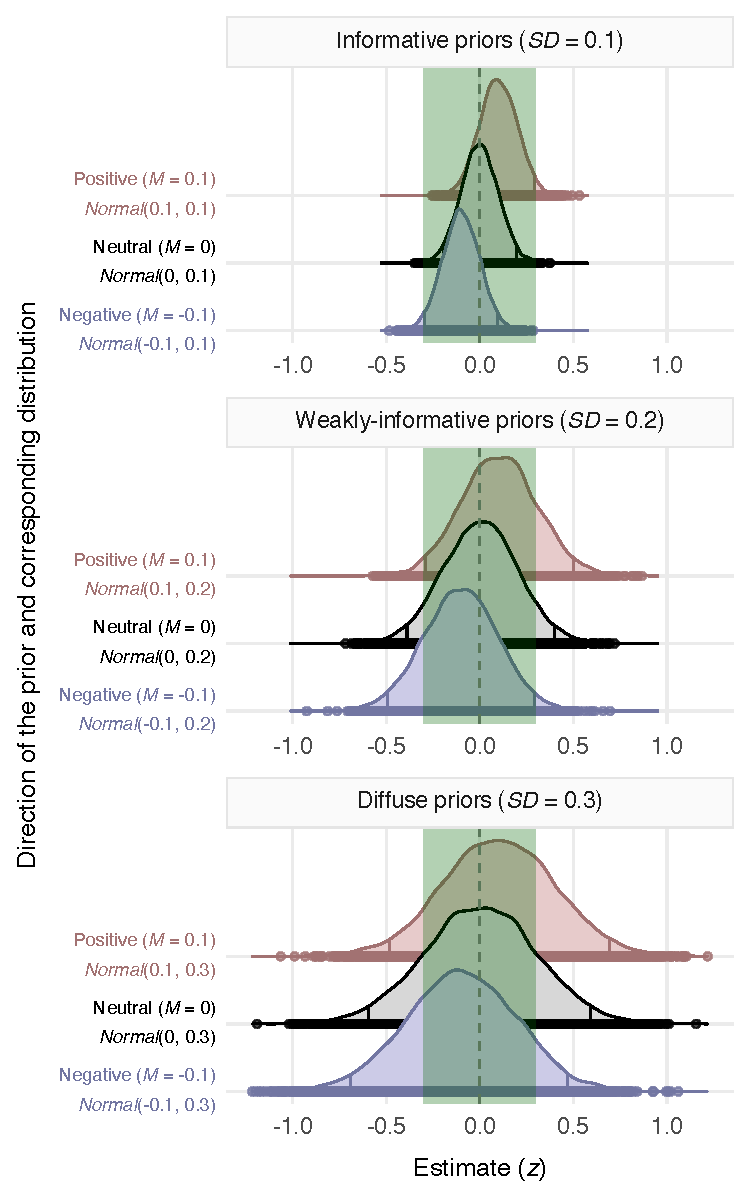
\includegraphics[width=1\linewidth]{C:/Users/Pablo/Documents/semanticpriming-semanticdecision-lexicaldecision/bayesian_priors/plots/bayesian_priors} 

}

\caption{Priors used in the three studies. The green vertical rectangle shows the range of plausible effect sizes based on previous studies and on our frequentist analyses. In the informative priors, around 95\% of the values fall within the range.}\label{fig:bayesian-priors}
\end{figure}

The adequacy of each of these priors was assessed by performing prior predictive checks, in which we compared the observed data to the predictions of the model (Schoot et al., 2021). Furthermore, in these checks we also tested the adequacy of two model-wide distributions: the traditional Gaussian distribution (default in most analyses) and an exponentially modified Gaussian---dubbed `ex-Gaussian'---distribution (Matzke \& Wagenmakers, 2009). The ex-Gaussian distribution was considered because the residual errors of the frequentist models were not normally distributed (Lo \& Andrews, 2015), and because this distribution was found to be more appropriate than the Gaussian one in a previous, related study (see supplementary materials of Rodríguez-Ferreiro et al., 2020). The ex-Gaussian distribution had an identity link function, which preserves the interpretability of the coefficients, as opposed to a transformation applied directly to the dependent variable (Lo \& Andrews, 2015). The results of these prior predictive checks revealed that the priors were adequate, and that the ex-Gaussian distribution was more appropriate than the Gaussian one (see \protect\hyperlink{appendix-C-Bayesian-analysis-diagnostics}{\underline{Appendix C}}), converging with Rodríguez-Ferreiro et al. (2020). Therefore, the ex-Gaussian distribution was used in the final models.

\hypertarget{prior-sensitivity-analysis}{%
\subparagraph{Prior sensitivity analysis}\label{prior-sensitivity-analysis}}

In the main analysis, the informative, weakly-informative and diffuse priors were used in separate models. In other words, in each model, all priors had the same degree of informativeness (as done in Pregla et al., 2021; Rodríguez-Ferreiro et al., 2020; Stone et al., 2021; Stone et al., 2020). In this way, a prior sensitivity analysis was performed to acknowledge the likely influence of the priors on the posterior distributions---that is, on the results (Lee \& Wagenmakers, 2014; Schoot et al., 2021; Stone et al., 2020).

\hypertarget{posterior-distributions}{%
\paragraph{Posterior distributions}\label{posterior-distributions}}

Posterior predictive checks were performed to assess the consistency between the observed data and new data predicted by the posterior distributions (Schoot et al., 2021). These checks are available in \protect\hyperlink{appendix-C-Bayesian-analysis-diagnostics}{\underline{Appendix C}}.

\hypertarget{convergence}{%
\paragraph{Convergence}\label{convergence}}

When convergence was not reached in a model, as indicated by \(\widehat R\) \textgreater{} 1.01 (Schoot et al., 2021; Vehtari et al., 2021), the number of iterations was increased and the random slopes for covariates were removed (Brauer \& Curtin, 2018). The resulting random effects in these models were largely the same as those present in the frequentist models. The only exception concerned the models of the lexical decision study. In the frequentist model for the latter study, the random slopes for covariates were removed due to convergence warnings, whereas in the Bayesian analysis, these random slopes did not have to be removed as the models converged, thanks to the large number of iterations that were run. In the lexical decision study, it was possible to run a larger number of iterations than in the two other studies, as the lexical decision data set had fewer observations, resulting in faster running.

The Bayesian models in the semantic decision study could not be made to converge, and the final results of these models were not valid. Therefore, those estimates are not shown in the main text, but are available in \protect\hyperlink{appendix-E-Bayesian-analysis-results}{\underline{Appendix E}}.

\hypertarget{statistical-power-analysis-1}{%
\subsection{Statistical power analysis}\label{statistical-power-analysis-1}}

Power curves based on Monte Carlo simulations were performed for most of the effects of interest using the R package `simr', Version 1.0.5 (Green \& MacLeod, 2016). Obtaining power curves for a range of effects in each study allows for a comprehensive assessment of the plausibility of the power estimated for each effect.

In each study, the item-level sample size---i.e., the number of words---was not modified. Therefore, to plan the sample size for future studies, these results must be considered under the assumptions that the future study would apply a statistical method similar to ours---namely, a mixed-effects model with random intercepts and slopes---, and that the analysis would encompass at least as many stimuli as the corresponding study (numbers detailed in each study below). \(P\) values were calculated using the Satterthwaite approximation for degrees of freedom (Luke, 2017).

Monte Carlo simulations consist of running the statistical model a large number of times, under slight, random variations of the dependent variable (Green \& MacLeod, 2016; for a comparable approach, see Loken \& Gelman, 2017). The power to detect each effect of interest is calculated by dividing the number of times that the effect is significant by the total number of simulations run. For instance, if an effect is significant on 85 simulations out of 100, the power for that effect is 85\% (Kumle et al., 2021). The sample sizes tested in the semantic priming study ranged from 50 to 800 participants, whereas those tested in the semantic decision and lexical decision studies ranged from 50 to 2,000 participants. These sample sizes were unequally spaced to limit the computational requirements. They comprised the following: 50, 100, 200, 300, 400, 500, 600, 700, 800, 1,200, 1,600 and 2,000 participants.\footnote{For the semantic priming study, the remaining sample sizes up to 2,000 participants have not finished running yet. Upon finishing, they will be reported in this manuscript.} The variance of the results decreases as more simulations are run. In each of our three studies, 200 simulations (as in Brysbaert \& Stevens, 2018) were run for each effect of interest and for each sample size under consideration. Thus, for a power curve examining the power for an effect across 12 sample sizes, 2,400 simulations were run.

Power analyses require setting an effect size for each effect. Often, it is difficult to determine the effect size, as the amount and the scope of relevant research are usually finite and biased (Albers \& Lakens, 2018; Gelman \& Carlin, 2014; Kumle et al., 2021). In some power analyses, the original effect sizes from previous studies have been adopted without any modification (e.g., Pacini \& Barnard, 2021; Villalonga et al., 2021). In contrast, some authors have opted to reduce the previous effect sizes to account for two intervening factors. First, publication bias and insufficient statistical power cause published effect sizes to be inflated (Brysbaert, 2019; Loken \& Gelman, 2017; Open Science Collaboration, 2015; Vasishth, Mertzen, et al., 2018; Vasishth \& Gelman, 2021). Second, over the course of the research, a variety of circumstances could create differences between the planned study and the studies that were used in the power analysis. Some of these differences could be foreseeable---for instance, if they are due to a limitation in the literature available for the power analysis---, whereas other differences might be unforeseeable and could go unnoticed (Barsalou, 2019; Noah et al., 2018). Reducing the effect size in the power analysis leads to an increase of the sample size of the planned study (Brysbaert \& Stevens, 2018; Green \& MacLeod, 2016; Hoenig \& Heisey, 2001). The reduced effect size---sometimes dubbed the smallest effect size of interest---is often set with a degree of arbitrariness. In previous studies, Fleur et al. (2020) applied a reduction of 1/8 (i.e., 12.5\%), whereas Kumle et al. (2021) applied a 15\% reduction. In the present study, a reduction of 20\% was applied to every effect in the power analysis. By comparison with the power analyses reviewed in this paragraph, the present reduction will lead to a more conservative estimate of required sample sizes. However, after considering the precedents of small samples and publication bias reviewed above, a 20\% reduction is arguably a reasonable safeguard. Indeed, a posteriori, the results of our power analyses suggested that the 20\% reduction had not been excessive, as some of the effects examined were detectable with small sample sizes.

Both the primary analysis and the power analysis were performed in R (R Core Team, 2021). Version 4.0.2 was used for the frequentist analysis, Version 4.1.0 was used for the Bayesian analysis, and Version 4.1.2 was used for fast operations such as data preprocessing and plotting. Given the complexity of these analyses, all the statistical and the power analyses were run on the High-End Computing facility at Lancaster University.\footnote{Information about this facility is available at \url{https://answers.lancaster.ac.uk/display/ISS/High+End+Computing+\%28HEC\%29+help}. Even though analysis jobs were run in parallel, some of the statistical analyses took four months to complete (specifically, one month for the final model to run, which was delayed due to three reasons: limited availability of machines, occasional cancellations of jobs to allow maintenance work on the machines, and lack of convergence of the models). Furthermore, the power analysis for the semantic priming study took six months (specifically, two months of running, with delays due to the limited availability of machines and occasional cancellations of jobs).}

\hypertarget{study-1-semantic-priming}{%
\section{Study 1: Semantic priming}\label{study-1-semantic-priming}}

The core data set in this study was that of the Semantic Priming Project (Hutchison et al., 2013; also see Yap et al., 2017). The study of Hutchison et al. (2013) comprised two tasks: lexical decision and naming. We limited our analysis to the lexical decision task because it was more relevant to a subsequent study that we were planning. In the lexical decision task, participants judged whether strings of letters constituted real words (e.g., \emph{building}) or nonwords (e.g.~\emph{gop}). Importantly, in each trial, the target word that participants assessed was preceded by a prime word. Participants were only required to provide a response regarding the \emph{target} word. The characteristic feature of the semantic priming paradigm is the analysis of responses to the targets as a function of the semantic relationship between the primes and the targets (Brunellière et al., 2017; de Wit \& Kinoshita, 2015; Hoedemaker \& Gordon, 2014).

In some studies, the association between prime and target words has been investigated in terms of related versus unrelated pairs (Lam et al., 2015; Pecher et al., 1998; Trumpp et al., 2013) and---in other studies---in terms of first- and second-order relationships (Hutchison et al., 2013). In contrast to these categorical associations, a third set of studies have measured the association between the prime and the target words using continuous estimates of text-based similarity (Günther et al., 2016a, 2016b; Hutchison et al., 2008; M. N. Jones et al., 2006; Lund et al., 1995; Lund \& Burgess, 1996; Mandera et al., 2017; McDonald \& Brew, 2002; Padó \& Lapata, 2007; Petilli et al., 2021; Wingfield \& Connell, 2022a). In one of these studies, Mandera et al. (2017) found that computational measures of similarity outperformed human-based associations at explaining language-based priming.

\hypertarget{language-vision-and-soa}{%
\subsection{Language, vision and SOA}\label{language-vision-and-soa}}

Priming associations beyond the linguistic realm have also been investigated, with early studies observing perceptual priming effects (Flores d'Arcais et al., 1985; Schreuder et al., 1984). Yet, those early findings were soon reframed by Pecher et al. (1998), who conducted a follow-up with an improved design, and observed vision-based priming only when the task was preceded by another task that required attention to visual features of concepts (Ostarek \& Huettig, 2017; also see Yee et al., 2012). Furthermore, two studies have failed to observe vision-based priming (Hutchison, 2003; Ostarek \& Huettig, 2017).

Nonetheless, a considerable number of studies have observed perceptual priming, even in the absence of a pretask. A set of these studies used the Conceptual Modality Switch paradigm, in which the primes and the targets are presented in separate, consecutive trials---e.g., \emph{Loud Welcome} → \emph{Fine Selection} (Bernabeu et al., 2017; Collins et al., 2011; Hald et al., 2011, 2013; Louwerse \& Connell, 2011; Lynott \& Connell, 2009; Pecher et al., 2003; Trumpp et al., 2013). The other set of studies implemented the more classic priming manipulation, whereby a prime word is briefly presented before the target word in each trial---e.g., \emph{Welcome} → \emph{Selection}. This design is more relevant to our present study, as it was used in the study we are revisiting (Hutchison et al., 2013). Below, we review studies that have used the \emph{prime} → \emph{target} design.

Lam et al. (2015) conducted a semantic priming experiment containing a lexical decision task, in which participants were instructed to assess whether the prime word and the target word in each trial were both real words. The semantic priming manipulation consisted of the following types of associations between the prime and the target words: (1) semantic association (e.g., bolt → screwdriver), (2) action association (e.g., housekey → screwdriver), (3) visual association (e.g., soldering iron → screwdriver), and (4) no association (e.g., charger → screwdriver). In addition, the following SOAs were compared: 500, 650, 800 and 1,400 ms. First, Lam et al.~observed priming effects of the semantic type with all SOAs. Second, the authors observed action-based priming with the SOAs of 500, 650 and 1,400 ms. Last, they observed vision-based priming only with the SOA of 1,400 ms. Overall, semantic---i.e., language-based---priming was more prevalent than visual and action priming. The greater role of language-based information converges with other semantic priming studies (Bottini et al., 2016; Lam et al., 2015; Pecher et al., 1998; Petilli et al., 2021), as well as with studies that used other paradigms (Banks et al., 2021; Kiela \& Bottou, 2014; Louwerse et al., 2015).

Similarly, the results of Lam et al. (2015) regarding the time course of language-based and vision-based priming were consistent with a wealth of literature observing that the influence of perceptual systems, such as vision, peaks later than the influence of the language system (Barsalou et al., 2008; Louwerse \& Connell, 2011; Santos et al., 2011). For instance, studies using electroencephalography have observed perceptual priming effects within 300 ms from the word onset. Thereafter, the perceptual priming effect increased (Amsel et al., 2014; Bernabeu et al., 2017), or it stabilised (Kiefer et al., 2022), or fluctuated (Amsel, 2011). Overall, these patterns reveal a gradual accumulation of information throughout word processing (also see Hauk, 2016), which is consistent with the integration of contextual information (see Hald et al., 2006).

In a more recent study, Petilli et al. (2021) revisited the data of Hutchison et al. (2013) using new variables that indexed language-based and vision-based associations between the prime and the target words. These variables had two important characteristics: (1) they were continuous rather than categorical (see Cohen, 1983; Günther et al., 2016a; Mandera et al., 2017), and (2) they were not dependent on human ratings (cf. Hutchison et al., 2008, 2013; Lam et al., 2015; Pecher et al., 1998). By this means, Petilli et al.~avoided the circularity problem (rarely addressed in studies) that arises (or may arise) when human-based ratings are used to explain human behaviour.

Petilli et al. (2021) operationalised word co-occurrence using text-based similarity (Mandera et al., 2017). Next, to operationalise vision-based similarity, the authors obtained images from ImageNet corresponding to each word (a minimum of 100 images per word), and trained vector representations on those images using neural networks (for related work, see Roads \& Love, 2020). The resulting computational measure of vision-based similarity was then validated against human-based ratings (Pecher et al., 1998), with a satisfactory result. In a concrete demonstration, Petilli et al.~show how vision-based similarity correctly concluded that drills were more visually similar to pistols than to screwdrivers, showing that the measure was not misled by functional similarity. In conclusion, using \texttt{language-based\ similarity} and \texttt{vision-based\ similarity}, Petilli et al.~investigated language-based and vision-based priming in two tasks---lexical decision and naming---and with both a short and a long SOA.

In lexical decision, the largest effect observed by Petilli et al. (2021) was that of language-based priming with the short SOA (200 ms). The second largest effect was that of language-based priming with the long SOA (1,200 ms). Next, the weakest, significant effect was that of vision-based priming with the short SOA. Last, there was no effect of vision-based priming with the long SOA. Petilli et al.~explained the absence of vision-based priming with the long SOA by contending that visual activation had likely decayed before participants processed the target words (also see Yee et al., 2011), owing to the limited semantic processing required for lexical decision (also see Balota \& Lorch, 1986; Becker et al., 1997; de Wit \& Kinoshita, 2015; Joordens \& Becker, 1997; Ostarek \& Huettig, 2017). Therefore, the authors suggested that perceptual simulation does \emph{not} peak before language-based processing in lexical decision, contrasting with the results of Lam et al. (2015) and with the results found in other tasks (Louwerse \& Connell, 2011; Santos et al., 2011; Simmons et al., 2008; also see Barsalou et al., 2008).

In the naming task, the largest effect observed by Petilli et al. (2021) was that of language-based priming with the long SOA. The second largest effect was that of language-based priming with the short SOA. Last, there was no effect of vision-based priming with either SOA. This finding contrasts with Connell and Lynott (2014), who found facilitatory effects of visual strength in both lexical decision and naming. Petilli et al.~explained the lack of vision-based priming in the naming task by alluding to the lower semantic depth of this task---compared to lexical decision---, and the mixture of visual and auditory processing in this task (also see Connell \& Lynott, 2014).

In conclusion, there is mixed evidence regarding the time course of language-based and vision-based information in conceptual processing, and particularly in semantic priming. First, regarding language, previous research predicts that language-based priming will have a larger effect with the short SOA than with the long one (Lam et al., 2015; Petilli et al., 2021). Second, regarding vision, three hypotheses are available: (a) more vision-based priming with the long SOA (Louwerse \& Connell, 2011; Santos et al., 2011; Simmons et al., 2008; also see Barsalou et al., 2008), (b) vision-based priming only with the short SOA (Petilli et al., 2021), and (c) no vision-based priming (Hutchison, 2003; Ostarek \& Huettig, 2017; Pecher et al., 1998; Yee et al., 2012).

\hypertarget{language-vision-and-vocabulary-size}{%
\subsection{Language, vision and vocabulary size}\label{language-vision-and-vocabulary-size}}

Next, we turn to considering the role of participants' vocabulary size with respect to language-based and vision-based information (this recaps the general \protect\hyperlink{hypotheses}{\underline{Hypotheses}} section). First, three hypotheses exist the interaction with language. On the one hand, some research predicts a larger effect of language-based priming in higher-vocabulary participants (Yap et al., 2017; also see Connell, 2019; Landauer et al., 1998; Louwerse et al., 2015; Paivio, 1990; Pylyshyn, 1973). On the other hand, other research has found the opposite pattern (Yap et al., 2009; also see Yap et al., 2012). Also relevant to these mixed findings is the notion that vocabulary knowledge is associated with increased attention to task-relevant variables (Pexman \& Yap, 2018). We hypothesised that language-based information---represented by \texttt{language-based\ similarity} in this study---was indeed important for present task, given its importance across the board (Banks et al., 2021; Kiela \& Bottou, 2014; Lam et al., 2015; Louwerse et al., 2015; Pecher et al., 1998; Petilli et al., 2021). Accordingly, the relevance hypothesis predicted that higher-vocabulary participants would present a larger priming effect.

To our knowledge, no previous studies have investigated the interaction between vision-based information and participants' vocabulary size. We entertained two hypotheses: (a) that lower-vocabulary participants would be more sensitive to visual strength than higher-vocabulary participants, thereby compensating for the disadvantage on the language side, and (b) that this interaction effect would be absent.

\hypertarget{the-present-study}{%
\subsection{The present study}\label{the-present-study}}

In the present study, we expanded on Petilli et al. (2021) by examining the role of participants' vocabulary size. In other regards, we used the same primary data set (Hutchison et al., 2013), and a language-based similarity measure that was very similar to that used by Petilli et al. (also created by Mandera et al., 2017). In contrast, our vision-based predictors differed. Whereas Petilli et al.~used a human-independent measure trained on images (see description above), we calculated the difference in visual strength (Lynott et al., 2020) between the prime and the target word in each trial.\footnote{These measures are compared at \protect\hyperlink{results-human-based-and-computational-measures-of-visual-information}{\underline{the end of the Results section}}.}

\hypertarget{methods}{%
\subsection{Methods}\label{methods}}

\hypertarget{semanticpriming-dataset}{%
\subsubsection{Data set}\label{semanticpriming-dataset}}

The data set was trimmed by removing rows that lacked values on any variable, and by also removing RTs that were more than 3 standard deviations away from the mean. The standard deviation trimming was performed within participants, within sessions and within SOA conditions, as done in the Semantic Priming Project (Hutchison et al., 2013). The resulting data set contained 496 participants, 5,943 prime--target pairs and 345,666 RTs. On average, there were 697 prime--target pairs per participant (\(SD\) = 33.34), and conversely, 58 participants per prime--target pair (\(SD\) = 4.25).

\hypertarget{variables}{%
\subsubsection{Variables}\label{variables}}

While the variables are generally described in the \protect\hyperlink{present-studies}{\underline{general introduction}}, a few further details are provided below regarding two of them.

\begin{itemize}
\item
  \texttt{Vocabulary\ size}. The test used by Hutchison et al. (2013) comprised a synonym test, an antonym test, and an analogy test, all three extracted from the Woodcock--Johnson III diagnostic reading battery (Woodcock et al., 2001). We operationalised the vocabulary measure as the mean score across the three tasks per participant.
\item
  \texttt{Language-based\ similarity}. This measure was calculated using a semantic space from Mandera et al. (2017), which the authors found to be the second-best predictor (\(R\)\textsuperscript{2} = .465) of the semantic priming effect in the lexical decision task of Hutchison et al. (2013) (we could not use the best semantic space, \(R\)\textsuperscript{2} = .471, owing to computational limitations). The second-best semantic space (see first row in Table 5 in Mandera et al., 2017) was based on lemmas from a subtitle corpus, and was processed using a Continuous Bag Of Words model. It had 300 dimensions and a window size of six words. The R package `LSAfun' (Günther et al., 2015) was used to import this variable.\footnote{Despite the name of the package, the measure we used was not based on Latent Semantic Analysis.}
\item
  \texttt{Stimulus\ onset\ asynchrony\ (SOA)}. Following Brauer and Curtin (2018), the categories of this factor were recoded as follows: 200 ms = -0.5, 1,200 ms = 0.5.
\end{itemize}

A few details regarding the covariates follow.

\begin{itemize}
\item
  \texttt{Attentional\ control} (Hutchison et al., 2013) was included as a measure akin to general cognition, and specifically as a covariate of vocabulary size (Ratcliff et al., 2010). The role of attentional control in semantic priming was evidenced by Yap et al. (2017). Attentional control comprised three attention-demanding tasks, namely, operation span, Stroop and antisaccade (Hutchison et al., 2013).
\item
  Lexical covariates (see \protect\hyperlink{appendix-A-lexical-covariates}{\underline{Appendix A}}): \texttt{word\ frequency} and \texttt{orthographic\ Levenshtein\ distance} (Balota et al., 2007).
\item
  \texttt{Word\ concreteness} (Brysbaert et al., 2014), used as a covariate of visual strength.
\end{itemize}

Figure \ref{fig:semanticpriming-correlations} shows the correlations among the predictors and the dependent variable.

\begin{figure}

{\centering 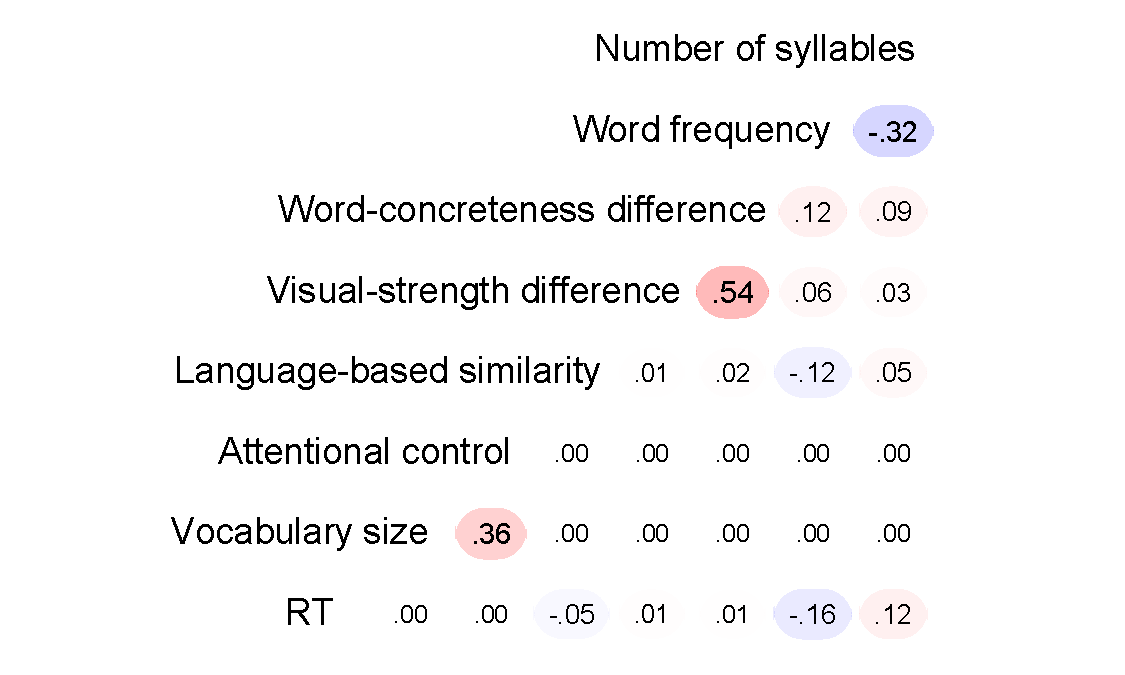
\includegraphics[width=0.65\linewidth]{manuscript_files/figure-latex/semanticpriming-correlations-1} 

}

\caption{Zero-order correlations in the semantic priming study.}\label{fig:semanticpriming-correlations}
\end{figure}

\hypertarget{diagnostics-for-the-frequentist-analysis}{%
\subsubsection{Diagnostics for the frequentist analysis}\label{diagnostics-for-the-frequentist-analysis}}

The model presented convergence warnings. To avoid removing important random slopes, which could increase the Type I error rate---i.e., false positives (Brauer \& Curtin, 2018; Singmann \& Kellen, 2019), we examined the model after refitting it using seven optimisation algorithms through the `allFit' function of the R package `lme4' (Bates et al., 2021). The results showed that all optimisers produced virtually identical means for all effects, suggesting that the convergence warnings were not consequential (Bates et al., 2021; see \protect\hyperlink{appendix-B-frequentist-analysis-diagnostics}{\underline{Appendix B}}).

The residual errors were not normally distributed, and attempts to mitigate this deviation proved unsuccessful (see \protect\hyperlink{appendix-B-frequentist-analysis-diagnostics}{\underline{Appendix B}}). However, this is not likely to have posed a major problem, as mixed-effects models are fairly robust to deviations from normality (Knief \& Forstmeier, 2021; Schielzeth et al., 2020). Last, the model did not present multicollinearity problems, with all variance inflation factors (VIF) below 2 (see Dormann et al., 2013; Harrison et al., 2018).

\hypertarget{diagnostics-for-the-bayesian-analysis}{%
\subsubsection{Diagnostics for the Bayesian analysis}\label{diagnostics-for-the-bayesian-analysis}}

Three Bayesian models were run that were respectively characterised by informative, weakly-informative and diffuse priors. In each model, 16 chains were used. In each chain, 1,500 warmup iterations were run, followed by 4,500 post-warmup iterations. Thus, a total of 72,000 post-warmup draws were produced over all the chains.

The maximum \(\widehat R\) value for the fixed effects across the three models was 1.00, suggesting that these parameters had converged (Schoot et al., 2021; Vehtari et al., 2021). In contrast, the maximum \(\widehat R\) value for the random effects was 1.13, slightly exceeding the 1.01 threshold (Vehtari et al., 2021). Since the interest of the present research is on the fixed effects, and the random effects were very close to convergence, the present model is valid.

The results of the posterior predictive checks were sound (see \protect\hyperlink{appendix-C-Bayesian-analysis-diagnostics}{\underline{Appendix C}}), indicating that the posterior distributions were sufficiently consistent with the observed data. Furthermore, in the prior sensitivity analysis, the results were virtually identical with the three priors that were considered (refer to the priors in Figure \ref{fig:bayesian-priors} above; to view the results in detail, see \protect\hyperlink{appendix-E-Bayesian-analysis-results}{\underline{Appendix E}}).

\hypertarget{semanticpriming-results}{%
\subsection{Results of Study 1}\label{semanticpriming-results}}

Table \ref{tab:semanticpriming-frequentist-model} presents the results. The fixed effects explained 4.22\% of the variance, and the random effects explained 11.01\% (Nakagawa et al., 2017). It is reasonable that random effects explain more variance, as they involve a far larger number of estimates for each effect. That is, whereas each fixed effect is formed of one estimate, the by-item random slopes for an individual difference variable---such as vocabulary size---comprise as many estimates as the number of stimulus items (in this study, the stimuli refer to the prime--target pairs).\footnote{For future reference, it should be noted that, in Studies 2 and 3, the \emph{stimuli} are the stimulus words, as there are no prime words in those studies.} Conversely, the by-participant random slopes for an item-level variable---such as language-based similarity---comprise as many estimates as the number of participants.

\begin{table}[!h]

\caption{\label{tab:semanticpriming-frequentist-model}Frequentist model for the semantic priming study.}
\centering
\begin{threeparttable}
\begin{tabular}[t]{lrrrrr}
\toprule
\multicolumn{1}{c}{ } & \multicolumn{1}{c}{$\upbeta$} & \multicolumn{1}{c}{$SE$} & \multicolumn{1}{c}{95\% CI} & \multicolumn{1}{c}{$t$} & \multicolumn{1}{c}{$p$}\\
\midrule
(Intercept) & 0.00 & 0.00 & {}[0.00, 0.01] & 1.59 & .112\\
\addlinespace[0.3em]
\multicolumn{6}{l}{\textbf{Individual differences}}\\
\cellcolor{gray!6}{\hspace{1em}Attentional control} & \cellcolor{gray!6}{0.00} & \cellcolor{gray!6}{0.00} & \cellcolor{gray!6}{{}[0.00, 0.00]} & \cellcolor{gray!6}{-0.56} & \cellcolor{gray!6}{.577}\\
\hspace{1em}Vocabulary size $^{\text{a}}$ & 0.00 & 0.00 & {}[0.00, 0.00] & 0.02 & .987\\
\hspace{1em}Gender $^{\text{a}}$ & 0.00 & 0.00 & {}[0.00, 0.00] & -0.03 & .979\\
\addlinespace[0.3em]
\multicolumn{6}{l}{\textbf{Target-word lexical covariates}}\\
\cellcolor{gray!6}{\hspace{1em}Word frequency} & \cellcolor{gray!6}{-0.16} & \cellcolor{gray!6}{0.00} & \cellcolor{gray!6}{{}[-0.16, -0.15]} & \cellcolor{gray!6}{-49.40} & \cellcolor{gray!6}{<.001}\\
\cellcolor{gray!6}{\hspace{1em}Number of syllables} & \cellcolor{gray!6}{0.07} & \cellcolor{gray!6}{0.00} & \cellcolor{gray!6}{{}[0.07, 0.08]} & \cellcolor{gray!6}{22.81} & \cellcolor{gray!6}{<.001}\\
\addlinespace[0.3em]
\multicolumn{6}{l}{\textbf{Prime--target relationship}}\\
\cellcolor{gray!6}{\hspace{1em}Word-concreteness difference} & \cellcolor{gray!6}{0.01} & \cellcolor{gray!6}{0.00} & \cellcolor{gray!6}{{}[0.01, 0.02]} & \cellcolor{gray!6}{3.48} & \cellcolor{gray!6}{.001}\\
\hspace{1em}Language-based similarity $^{\text{b}}$ & -0.08 & 0.00 & {}[-0.08, -0.07] & -22.44 & <.001\\
\hspace{1em}Visual-strength difference $^{\text{b}}$ & 0.01 & 0.00 & {}[0.01, 0.02] & 4.18 & <.001\\
\addlinespace[0.3em]
\multicolumn{6}{l}{\textbf{Task condition}}\\
\hspace{1em}Stimulus onset asynchrony (SOA) $^{\text{b}}$ & 0.06 & 0.01 & {}[0.04, 0.07] & 7.47 & <.001\\
\addlinespace[0.3em]
\multicolumn{6}{l}{\textbf{Interactions}}\\
\cellcolor{gray!6}{\hspace{1em}\makecell[l]{Word-concreteness difference  $\times$ \\ \hspace{0.3cm} Vocabulary size}} & \cellcolor{gray!6}{0.00} & \cellcolor{gray!6}{0.00} & \cellcolor{gray!6}{{}[0.00, 0.01]} & \cellcolor{gray!6}{1.31} & \cellcolor{gray!6}{.189}\\
\cellcolor{gray!6}{\hspace{1em}Word-concreteness difference  $\times$  SOA} & \cellcolor{gray!6}{0.00} & \cellcolor{gray!6}{0.00} & \cellcolor{gray!6}{{}[0.00, 0.01]} & \cellcolor{gray!6}{2.57} & \cellcolor{gray!6}{.010}\\
\cellcolor{gray!6}{\hspace{1em}Word-concreteness difference  $\times$  Gender} & \cellcolor{gray!6}{0.00} & \cellcolor{gray!6}{0.00} & \cellcolor{gray!6}{{}[-0.01, 0.00]} & \cellcolor{gray!6}{-0.97} & \cellcolor{gray!6}{.332}\\
\cellcolor{gray!6}{\hspace{1em}\makecell[l]{Language-based similarity  $\times$ \\ \hspace{0.3cm} Attentional control}} & \cellcolor{gray!6}{-0.01} & \cellcolor{gray!6}{0.00} & \cellcolor{gray!6}{{}[-0.01, 0.00]} & \cellcolor{gray!6}{-2.46} & \cellcolor{gray!6}{.014}\\
\cellcolor{gray!6}{\hspace{1em}\makecell[l]{Visual-strength difference  $\times$ \\ \hspace{0.3cm} Attentional control}} & \cellcolor{gray!6}{0.00} & \cellcolor{gray!6}{0.00} & \cellcolor{gray!6}{{}[0.00, 0.00]} & \cellcolor{gray!6}{0.24} & \cellcolor{gray!6}{.810}\\
\hspace{1em}\makecell[l]{Language-based similarity  $\times$ \\ \hspace{0.3cm} Vocabulary size} & -0.01 & 0.00 & {}[-0.01, 0.00] & -2.34 & .020\\
\hspace{1em}\makecell[l]{Visual-strength difference  $\times$ \\ \hspace{0.3cm} Vocabulary size} & 0.00 & 0.00 & {}[-0.01, 0.00] & -1.37 & .172\\
\hspace{1em}Language-based similarity  $\times$  Gender & 0.00 & 0.00 & {}[-0.01, 0.00] & -0.79 & .433\\
\hspace{1em}Visual-strength difference  $\times$  Gender & 0.00 & 0.00 & {}[0.00, 0.01] & 1.46 & .144\\
\hspace{1em}Language-based similarity  $\times$  SOA $^{\text{b}}$ & 0.01 & 0.00 & {}[0.00, 0.01] & 3.22 & .001\\
\hspace{1em}Visual-strength difference  $\times$  SOA $^{\text{b}}$ & 0.00 & 0.00 & {}[-0.01, 0.00] & -2.25 & .025\\
\bottomrule
\end{tabular}
\begin{tablenotes}
\item \textit{\linebreak} 
\item \textit{Note}. $\upbeta$ = Estimate based on $z$-scored predictors; \textit{SE} = standard error; \linebreak \phantom{.}CI = confidence interval. Shaded rows contain covariates. Some interactions are \linebreak \phantom{.}split over two lines, with the second line indented. \linebreak \linebreak \phantom{.}$^{\text{a}}$ By-word random slopes were included for this effect. \linebreak \phantom{.}$^{\text{b}}$ By-participant random slopes were included for this effect.
\end{tablenotes}
\end{threeparttable}
\end{table}

Both language-based similarity and visual-strength difference produced significant main effects. As expected, their effects had opposite directions. On the one hand, higher values of language-based similarity facilitated participants' performance, as reflected in shorter RTs. On the other hand, higher values of visual-strength difference led to longer RTs. Furthermore, language-based similarity interacted with vocabulary size and with SOA. There were no effects of participants' gender (see interaction figures below).

The effect sizes of language-based similarity and its interactions were larger than those of visual-strength difference. Figure \ref{fig:semanticpriming-frequentist-bayesian-plot-weaklyinformativepriors-exgaussian} displays the frequentist and the Bayesian estimates, which are broadly similar. The Bayesian estimates are from the weakly-informative prior model. The estimates of the two other models, based on informative and diffuse priors, were virtually identical to these (see \protect\hyperlink{appendix-E-Bayesian-analysis-results}{\underline{Appendix E}}).

\FloatBarrier

\begin{figure}

{\centering 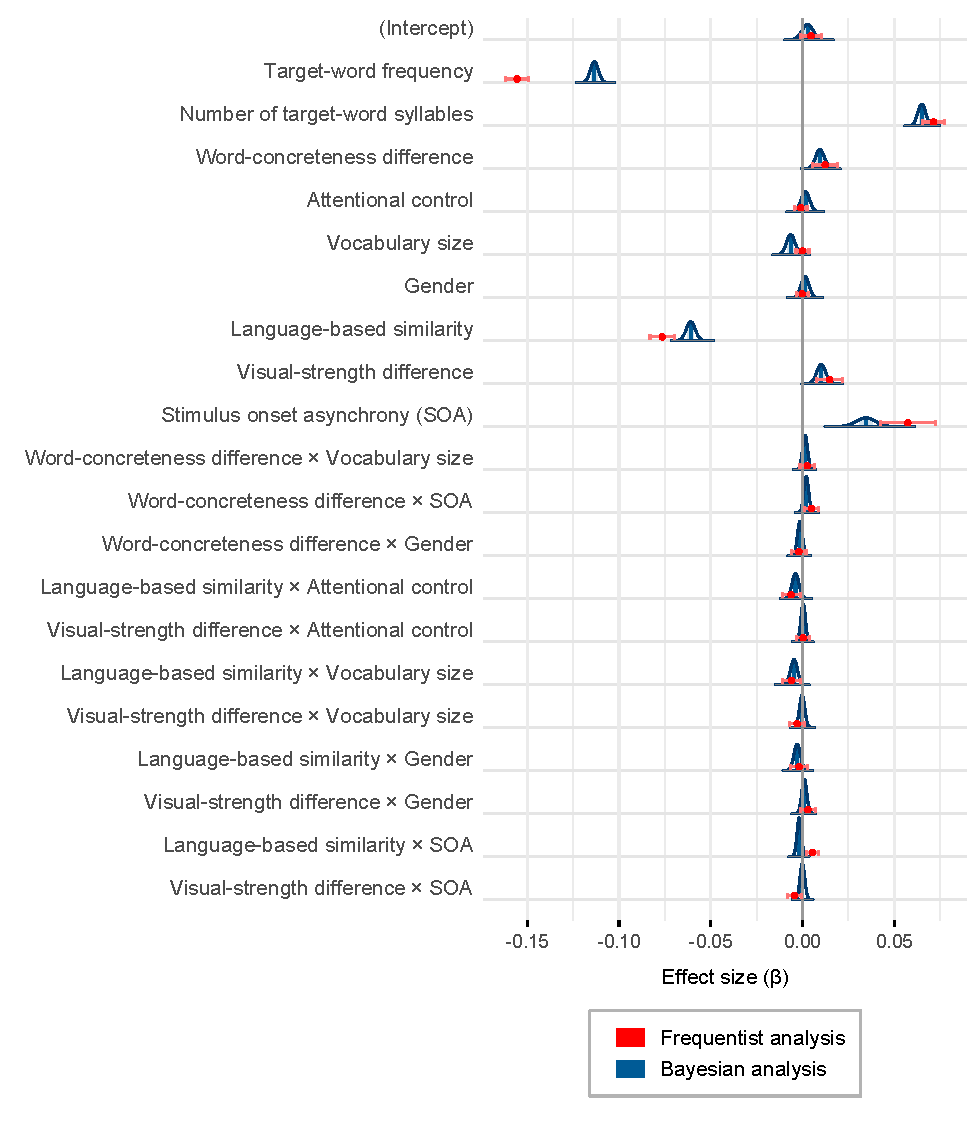
\includegraphics[width=1\linewidth]{C:/Users/Pablo/Documents/semanticpriming-semanticdecision-lexicaldecision/semanticpriming/frequentist_bayesian_plots/plots/semanticpriming_frequentist_bayesian_plot_weaklyinformativepriors_exgaussian} 

}

\caption{Estimates for the semantic priming study. The frequentist means (represented by red points) are flanked by 95\% confidence intervals. The Bayesian means (represented by blue vertical lines) are flanked by 95\% credible intervals in light blue.}\label{fig:semanticpriming-frequentist-bayesian-plot-weaklyinformativepriors-exgaussian}
\end{figure}

Figure \ref{fig:semanticpriming-interactions-with-vocabulary-size}-a shows the significant interaction between language-based similarity and vocabulary size, whereby higher-vocabulary participants presented a greater benefit from the language-based similarity between prime and target words. This interaction replicates the results of Yap et al. (2017), who analysed the same data set but using a categorical measure of similarity instead. Indeed, this replication is noteworthy as it holds in spite of some methodological differences between the studies. First, Yap et al. (2017) operationalised the priming effect as a categorical difference between related and unrelated prime--target pairs, which were based on association ratings produced by people (Nelson et al., 2004). In contrast, the present study applied a continuous measure of relatedness---i.e., cosine similarity---, which is more precise and may thus afford more statistical power (Mandera et al., 2017; Petilli et al., 2021). Therefore, this interaction demonstrates the consistency between human ratings and computational approximations to meaning (Charbonnier \& Wartena, 2019, 2020; Günther et al., 2016b; Louwerse et al., 2015; Mandera et al., 2017; Petilli et al., 2021; Solovyev, 2021; Wingfield \& Connell, 2022a). The second difference between the present study and Yap et al. (2017) is that Yap et al. (2017) performed a correlational analysis, whereas the present analysis used maximal mixed-effects models that included several covariates to measure the effects of interest as rigorously as possible.

Figure \ref{fig:semanticpriming-interactions-with-vocabulary-size}-b presents the non-significant interaction between visual-strength difference and vocabulary size.\footnote{All interaction plots across the three studies are based on the frequentist models. Further interaction plots available in \protect\hyperlink{appendix-D-interaction-plots}{\underline{Appendix D}}.} Albeit a non-significant interaction, the effect of visual-strength difference was larger in lower-vocabulary participants.



\begin{figure}

{\centering 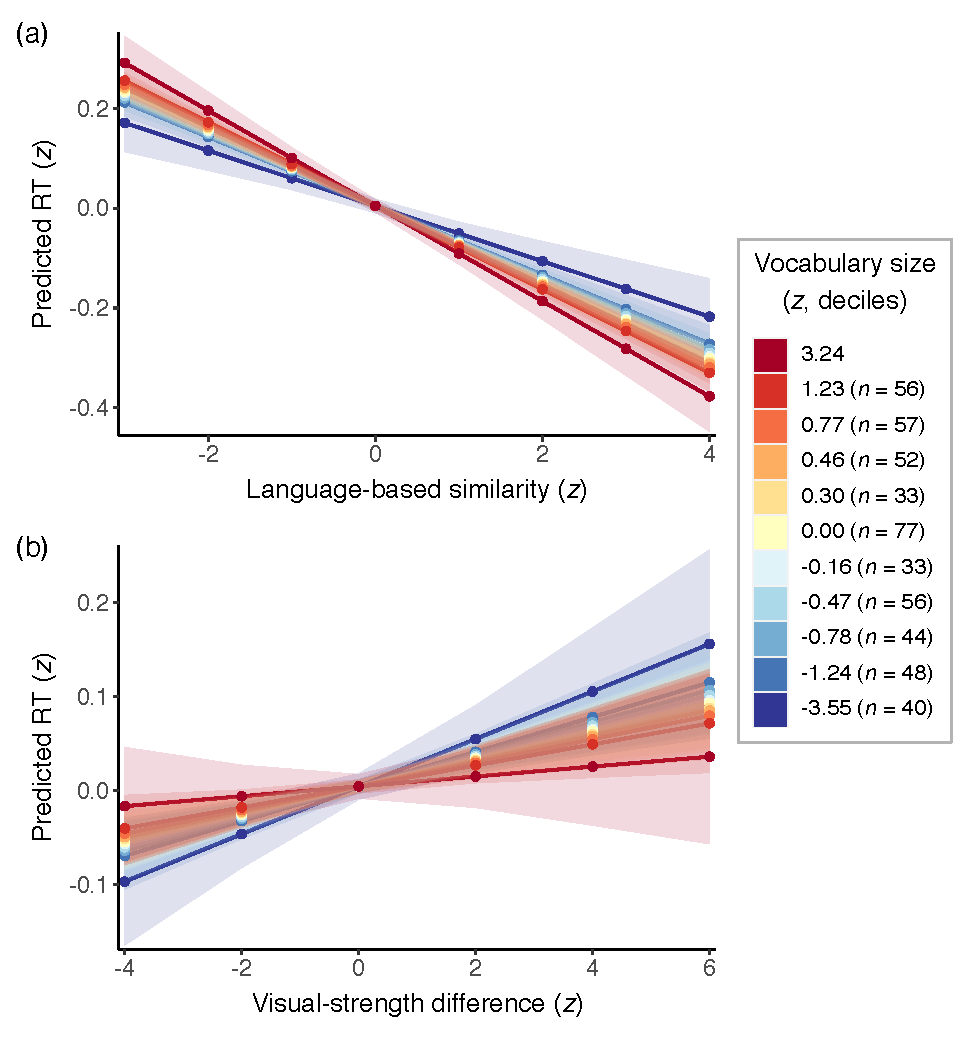
\includegraphics[width=0.85\linewidth]{C:/Users/Pablo/Documents/semanticpriming-semanticdecision-lexicaldecision/semanticpriming/frequentist_analysis/plots/semanticpriming-interactions-with-vocabulary-size} 

}

\caption{Interactions of vocabulary size with language-based similarity (panel a) and with visual-strength difference (panel b). Vocabulary size is constrained to deciles (10 sections) in this plot, whereas in the statistical analysis it contained more values within the current range. \(n\) = number of participants contained between deciles.}\label{fig:semanticpriming-interactions-with-vocabulary-size}
\end{figure}

Figure \ref{fig:semanticpriming-interactions-with-SOA} shows that the effects of language-based similarity and visual-strength difference were both larger with the short SOA. However, whereas the effect of language-based similarity was present with both SOAs (i.e., 200 ms and 1,200 ms), the effect of visual-strength difference was almost exclusive to the the long SOA. These results are consistent with Petilli et al. (2021), whereas they contrast with previous findings regarding the slower pace of the visual system in semantic priming (Lam et al., 2015) and in other paradigms (Louwerse \& Connell, 2011).

\begin{figure}

{\centering 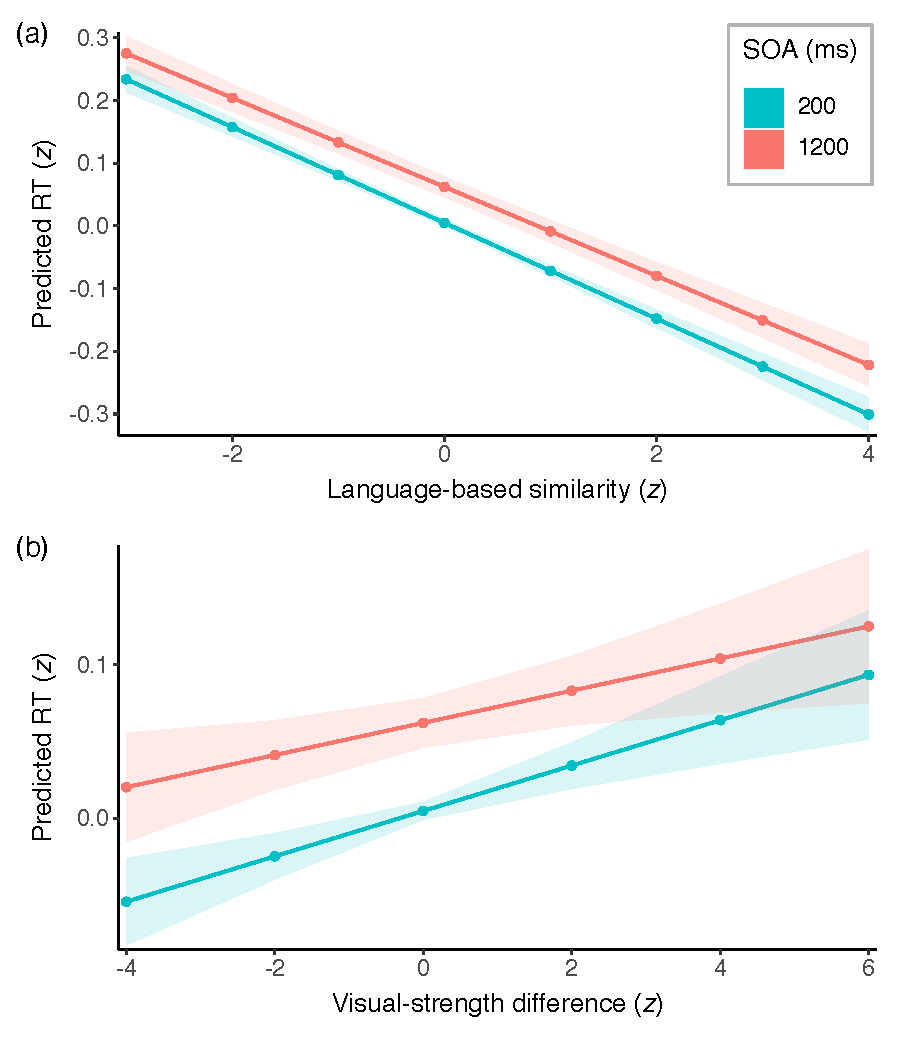
\includegraphics[width=0.8\linewidth]{C:/Users/Pablo/Documents/semanticpriming-semanticdecision-lexicaldecision/semanticpriming/frequentist_analysis/plots/semanticpriming-interactions-with-SOA} 

}

\caption{Interactions of stimulus onset asynchrony (SOA) with language-based similarity (panel a) and with visual-strength difference (panel b) in the semantic priming study. SOA was analysed using $z$-scores, but for clarity, the basic labels are used in the legend.}\label{fig:semanticpriming-interactions-with-SOA}
\end{figure}

Figure \ref{fig:semanticpriming-interactions-with-gender} shows the non-significant interactions of gender with language-based similarity and with visual-strength difference.

\begin{figure}

{\centering 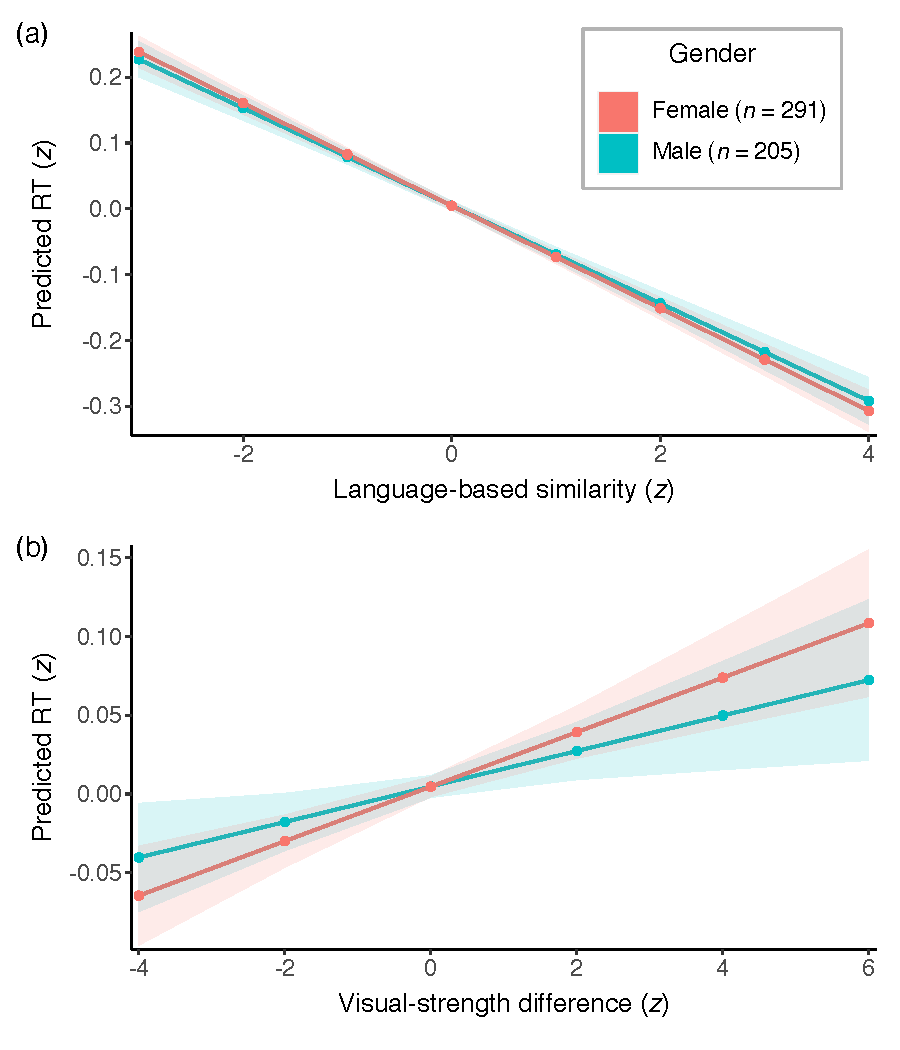
\includegraphics[width=0.8\linewidth]{C:/Users/Pablo/Documents/semanticpriming-semanticdecision-lexicaldecision/semanticpriming/frequentist_analysis/plots/semanticpriming-interactions-with-gender} 

}

\caption{Interactions of gender with language-based similarity (panel a) and with visual-strength difference (panel b) in the semantic priming study. Gender was analysed using $z$-scores, but for clarity, the basic labels are used in the legend.}\label{fig:semanticpriming-interactions-with-gender}
\end{figure}

\hypertarget{results-human-based-and-computational-measures-of-visual-information}{%
\subsubsection{Human-based and computational measures of visual information}\label{results-human-based-and-computational-measures-of-visual-information}}

Next, we reflected on the adequacy of visual-strength difference as a measurement instrument, as it had never (to our knowledge) been used before in the study of semantic priming. Even though the effect of this variable on task performance was---as expected---inhibitory (i.e., higher values of this variable leading to longer RTs), we were concerned about the low correlation between visual-strength difference and language-based similarity (\(r\) = .01). First, the negligible size of this correlation raised concerns, as we expected a larger and negative correlation. Second, Petilli et al. (2021) had found a correlation of \(r\) = .50 between vision-based similarity and language-based similarity. This prompted us to compare the performance of our measure---i.e., \texttt{visual-strength\ difference}---to that of Petilli et al.---i.e., \texttt{vision-based\ similarity}.

For this purpose, we first subsetted our previous data set to ensure that all trials contained data from all relevant variables---i.e., from all the existing variables and from the newly-added \texttt{vision-based\ similarity} from Petilli et al. (2021). This process resulted in the loss of 83\% of trials, owing to the strict selection criteria that had been applied by Petilli et al.~in the creation of their variable---for instance, both the target and the prime word had to be associated to at least 100 pictures in ImageNet. The rest of the preprocessing involved the same steps as the main analysis (detailed in \protect\hyperlink{semanticpriming-dataset}{\underline{Methods}}). The resulting data set contained 496 participants, 1,091 prime--target pairs and 254,140 RTs. On average, there were 128 prime--target pairs per participant (\(SD\) = 10.37), and conversely, 58 participants per prime--target pair (\(SD\) = 4.90).

Figure \ref{fig:semanticpriming-with-visualsimilarity-correlations} shows the correlations among the predictors and the dependent variable.

\begin{figure}

{\centering 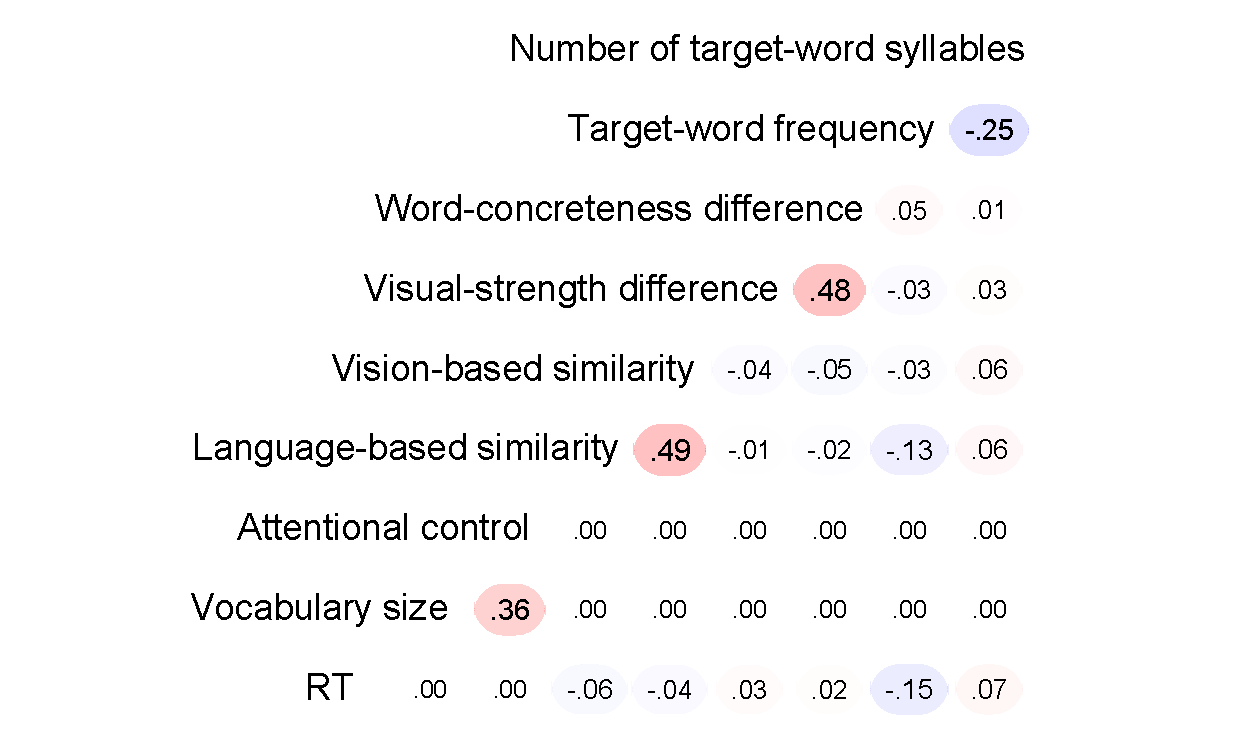
\includegraphics[width=0.73\linewidth]{manuscript_files/figure-latex/semanticpriming-with-visualsimilarity-correlations-1} 

}

\caption{Zero-order correlations in the semantic priming data set that included vision-based similarity.}\label{fig:semanticpriming-with-visualsimilarity-correlations}
\end{figure}

\hypertarget{diagnostics-for-the-frequentist-analysis-1}{%
\subsubsection{Diagnostics for the frequentist analysis}\label{diagnostics-for-the-frequentist-analysis-1}}

The model presented convergence warnings. To avoid removing important random slopes, which could increase the Type I error rate---i.e., false positives (Brauer \& Curtin, 2018; Singmann \& Kellen, 2019), we examined the model after refitting it using seven optimisation algorithms through the `allFit' function of the `lme4' package (Bates et al., 2021). The results showed that all optimisers produced virtually identical means for all effects, suggesting that the convergence warnings were not consequential (Bates et al., 2021; see \protect\hyperlink{appendix-B-frequentist-analysis-diagnostics}{\underline{Appendix B}}).

The residual errors were not normally distributed, and attempts to mitigate this deviation proved unsuccessful (see \protect\hyperlink{appendix-B-frequentist-analysis-diagnostics}{\underline{Appendix B}}). However, this is not likely to have posed a major problem, as mixed-effects models are fairly robust to deviations from normality (Knief \& Forstmeier, 2021; Schielzeth et al., 2020). Last, the model did not present multicollinearity problems, with all VIFs below 2 (see Dormann et al., 2013; Harrison et al., 2018).

\hypertarget{results}{%
\paragraph{Results}\label{results}}

Table \ref{tab:semanticpriming-with-visualsimilarity-frequentist-model} presents the results. Due to space, the covariates are shown in Table \ref{tab:semanticpriming-with-visualsimilarity-frequentist-model-covariates}. The fixed effects explained 3.53\% of the variance, and the random effects explained 18.47\% (Nakagawa et al., 2017; for an explanation of this difference, see \protect\hyperlink{semanticpriming-results}{\underline{Results of Study 1}}). Figure \ref{fig:semanticpriming-with-visualsimilarity-confidence-intervals-plot} displays the frequentist estimates of the effects of interest (Bayesian estimates not computed due to time constraints).

\begin{table}[!h]

\caption{\label{tab:semanticpriming-with-visualsimilarity-frequentist-model}Effects of interest in the semantic priming model that included vision-based similarity.}
\centering
\begin{threeparttable}
\begin{tabular}[t]{lrrrrr}
\toprule
\multicolumn{1}{c}{ } & \multicolumn{1}{c}{$\upbeta$} & \multicolumn{1}{c}{$SE$} & \multicolumn{1}{c}{95\% CI} & \multicolumn{1}{c}{$t$} & \multicolumn{1}{c}{$p$}\\
\midrule
(Intercept) & 0.01 & 0.01 & {}[-0.01, 0.02] & 0.90 & .370\\
\addlinespace[0.3em]
\multicolumn{6}{l}{\textbf{Individual differences}}\\
\hspace{1em}Vocabulary size $^{\text{a}}$ & 0.00 & 0.00 & {}[-0.01, 0.01] & 0.21 & .834\\
\hspace{1em}Gender $^{\text{a}}$ & 0.00 & 0.00 & {}[-0.01, 0.01] & -0.05 & .962\\
\addlinespace[0.3em]
\multicolumn{6}{l}{\textbf{Prime--target relationship}}\\
\hspace{1em}Language-based similarity $^{\text{b}}$ & -0.07 & 0.01 & {}[-0.09, -0.06] & -8.33 & <.001\\
\hspace{1em}Visual-strength difference $^{\text{b}}$ & 0.03 & 0.01 & {}[0.01, 0.04] & 3.04 & .002\\
\hspace{1em}Vision-based similarity $^{\text{b}}$ & -0.02 & 0.01 & {}[-0.04, -0.01] & -2.55 & .011\\
\addlinespace[0.3em]
\multicolumn{6}{l}{\textbf{Task condition}}\\
\hspace{1em}Stimulus onset asynchrony (SOA) $^{\text{b}}$ & 0.06 & 0.01 & {}[0.04, 0.08] & 6.80 & <.001\\
\addlinespace[0.3em]
\multicolumn{6}{l}{\textbf{Interactions}}\\
\hspace{1em}\makecell[l]{Language-based similarity  $\times$ \\ \hspace{0.3cm} Vocabulary size} & -0.01 & 0.01 & {}[-0.02, 0.01] & -0.96 & .339\\
\hspace{1em}\makecell[l]{Visual-strength difference  $\times$ \\ \hspace{0.3cm} Vocabulary size} & -0.01 & 0.01 & {}[-0.02, 0.01] & -1.02 & .309\\
\hspace{1em}\makecell[l]{Vision-based similarity  $\times$ \\ \hspace{0.3cm} Vocabulary size} & 0.00 & 0.01 & {}[-0.01, 0.01] & -0.01 & .991\\
\hspace{1em}Language-based similarity  $\times$  Gender & 0.00 & 0.01 & {}[-0.02, 0.01] & -0.75 & .456\\
\hspace{1em}Visual-strength difference  $\times$  Gender & -0.01 & 0.01 & {}[-0.02, 0.01] & -1.05 & .294\\
\hspace{1em}Vision-based similarity  $\times$  Gender & 0.00 & 0.01 & {}[-0.01, 0.01] & 0.39 & .696\\
\hspace{1em}Language-based similarity  $\times$  SOA $^{\text{b}}$ & 0.00 & 0.00 & {}[0.00, 0.01] & 0.87 & .382\\
\hspace{1em}Visual-strength difference  $\times$  SOA $^{\text{b}}$ & -0.01 & 0.00 & {}[-0.02, 0.00] & -2.60 & .010\\
\hspace{1em}Vision-based similarity  $\times$  SOA $^{\text{b}}$ & 0.01 & 0.00 & {}[0.00, 0.01] & 1.28 & .201\\
\bottomrule
\end{tabular}
\begin{tablenotes}
\item \textit{\linebreak} 
\item \textit{Note}. $\upbeta$ = Estimate based on $z$-scored predictors; \textit{SE} = standard error; \linebreak \phantom{.}CI = confidence interval. Covariates shown in next table due to space. Some  \linebreak \phantom{.}interactions are split over two lines, with the second line indented. \linebreak \linebreak \phantom{.}$^{\text{a}}$ By-word random slopes were included for this effect. \linebreak \phantom{.}$^{\text{b}}$ By-participant random slopes were included for this effect.
\end{tablenotes}
\end{threeparttable}
\end{table}

\begin{table}[!h]

\caption{\label{tab:semanticpriming-with-visualsimilarity-frequentist-model-covariates}Covariates in the semantic priming model that included vision-based similarity.}
\centering
\begin{threeparttable}
\begin{tabular}[t]{lrrrrr}
\toprule
\multicolumn{1}{c}{ } & \multicolumn{1}{c}{$\upbeta$} & \multicolumn{1}{c}{$SE$} & \multicolumn{1}{c}{95\% CI} & \multicolumn{1}{c}{$t$} & \multicolumn{1}{c}{$p$}\\
\midrule
\addlinespace[0.3em]
\multicolumn{6}{l}{\textbf{Individual difference covariate}}\\
\hspace{1em}Attentional control & 0.00 & 0.00 & {}[-0.01, 0.00] & -1.06 & .288\\
\addlinespace[0.3em]
\multicolumn{6}{l}{\textbf{Target-word lexical covariates}}\\
\hspace{1em}Word frequency & -0.15 & 0.01 & {}[-0.17, -0.14] & -21.97 & <.001\\
\hspace{1em}Number of syllables & 0.02 & 0.01 & {}[0.01, 0.04] & 3.54 & <.001\\
\addlinespace[0.3em]
\multicolumn{6}{l}{\textbf{Prime--target covariate}}\\
\hspace{1em}Word-concreteness difference & 0.02 & 0.01 & {}[0.01, 0.04] & 2.73 & .006\\
\addlinespace[0.3em]
\multicolumn{6}{l}{\textbf{Covariate interactions}}\\
\hspace{1em}\makecell[l]{Word-concreteness difference  $\times$ \\ \hspace{0.3cm} Vocabulary size} & -0.01 & 0.00 & {}[-0.01, 0.00] & -1.15 & .252\\
\hspace{1em}Word-concreteness difference  $\times$  SOA & 0.01 & 0.00 & {}[0.01, 0.02] & 5.64 & <.001\\
\hspace{1em}Word-concreteness difference  $\times$  Gender & 0.01 & 0.00 & {}[0.00, 0.01] & 1.34 & .179\\
\hspace{1em}\makecell[l]{Language-based similarity  $\times$ \\ \hspace{0.3cm} Attentional control} & 0.00 & 0.00 & {}[-0.01, 0.01] & -0.91 & .362\\
\hspace{1em}\makecell[l]{Visual-strength difference  $\times$ \\ \hspace{0.3cm} Attentional control} & 0.00 & 0.00 & {}[-0.01, 0.01] & 0.71 & .477\\
\hspace{1em}\makecell[l]{Vision-based similarity  $\times$ \\ \hspace{0.3cm} Attentional control} & 0.00 & 0.00 & {}[-0.01, 0.01] & 0.80 & .423\\
\bottomrule
\end{tabular}
\begin{tablenotes}
\item \textit{\linebreak} 
\item \textit{Note}. $\upbeta$ = Estimate based on $z$-scored predictors; \textit{SE} = standard error; \linebreak \phantom{.}CI = confidence interval. Some interactions are split over two lines, with the \linebreak \phantom{.}second line indented. \linebreak
\end{tablenotes}
\end{threeparttable}
\end{table}

\FloatBarrier

\begin{figure}

{\centering 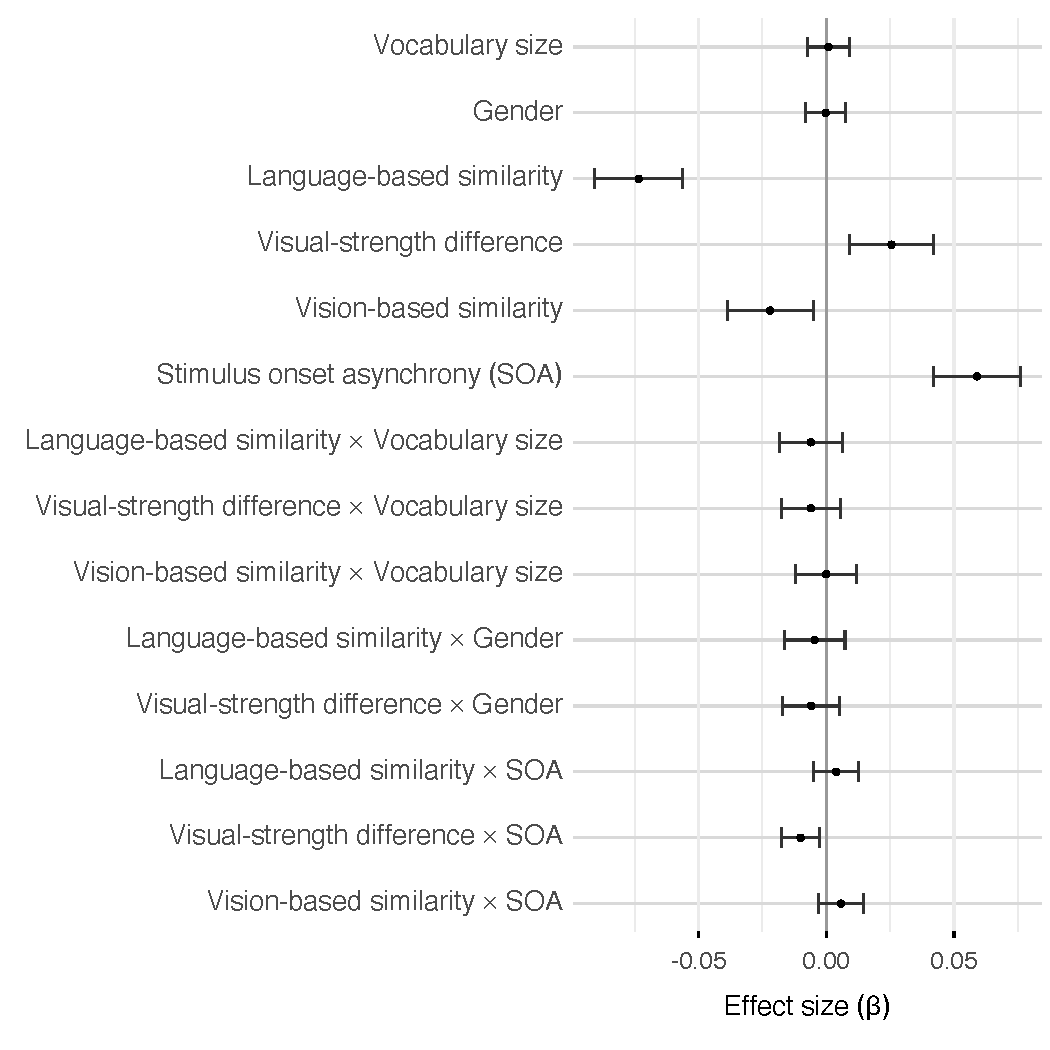
\includegraphics[width=0.89\linewidth]{C:/Users/Pablo/Documents/semanticpriming-semanticdecision-lexicaldecision/semanticpriming/analysis_with_visualsimilarity/plots/semanticpriming_with_visualsimilarity_confidence_intervals_plot} 

}

\caption{Means and 95\% confidence intervals for the effects of interest in the semantic priming model that included vision-based similarity.}\label{fig:semanticpriming-with-visualsimilarity-confidence-intervals-plot}
\end{figure}

The results revealed an effect of the human-based measure, \texttt{visual-strength\ difference} (as in the main analysis above), along with a smaller effect of the computational measure, \texttt{vision-based\ similarity}. There was an important difference between these measures regarding the interaction with SOA. Whereas visual-strength difference had a larger effect with the short SOA, vision-based similarity did not interact with SOA, contrary to the results of Petilli et al. (2021). This difference was not due to collinearity between these measures (\(r\) = -.04). Also importantly, both measures appeared to be valid based on their correlations with language-based similarity and with word concreteness (Figure \ref{fig:semanticpriming-with-visualsimilarity-correlations}). We reflect on this result in the discussion.

\hypertarget{statistical-power-analysis-2}{%
\subsubsection{Statistical power analysis}\label{statistical-power-analysis-2}}

Power curves were performed for most effects of interest in the main model. This was done using the main model, not the follow-up that included vision-based similarity. Figures \ref{fig:semanticpriming-powercurve-plots-1-2-3} and \ref{fig:semanticpriming-powercurve-plots-4-5-6-7-8-9} show the estimated power for some main effects and interactions of interest as a function of the number of participants. To plan the sample size for future studies, these results must be considered under the assumptions that the future study would apply a statistical method similar to ours---namely, a mixed-effects model with random intercepts and slopes---, and that the analysis would encompass at least as many prime--target pairs as the current study, namely, 5,943 (distributed in various blocks across participants, not all being presented to every participant). Furthermore, it is necessary to consider each figure in detail. Here, we provide a summary. First, detecting the main effect of language-based similarity---which had a strong effect on RTs---would require 50 participants. Second, detecting the interaction between language-based similarity and SOA---which was a considerably weaker effect---would require 600 participants. Last, the other effects would require more than 1,000 participants---or, in the case of gender differences, many more than that.

\begin{figure}

{\centering 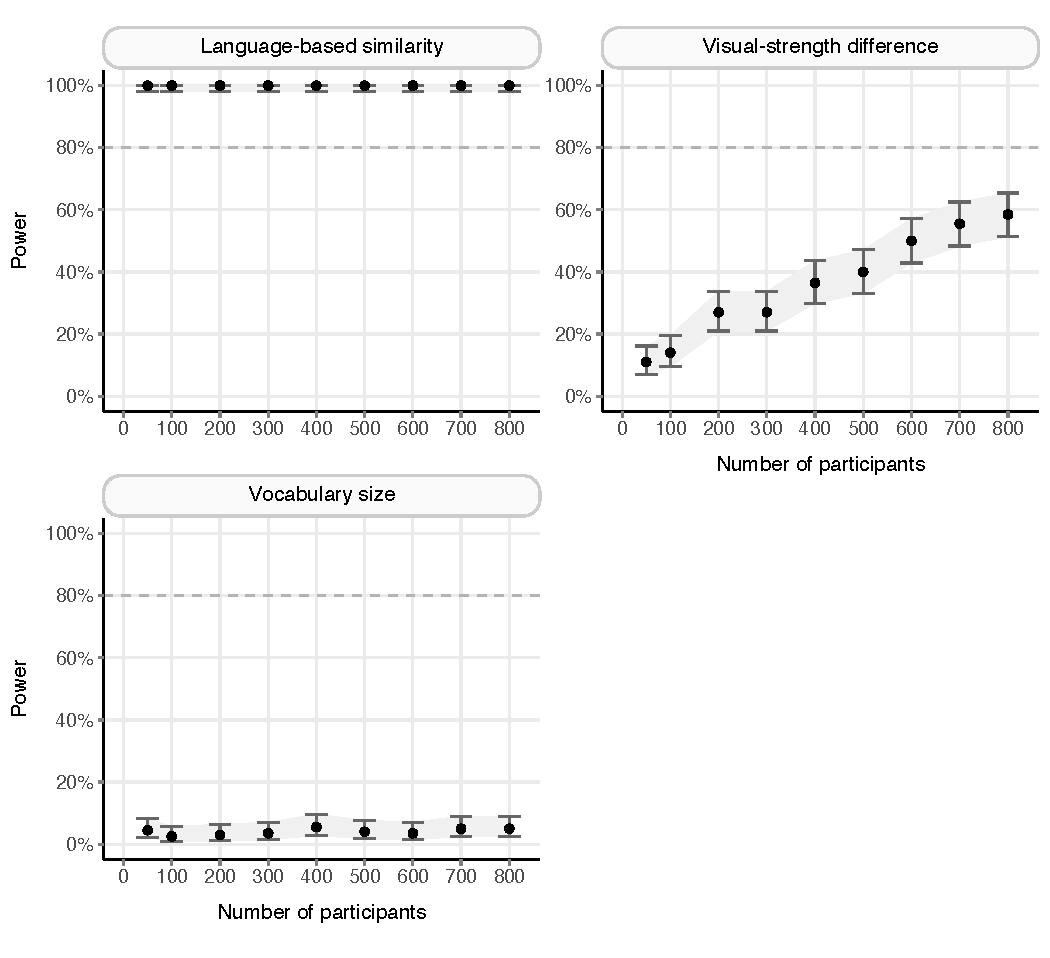
\includegraphics[width=1\linewidth]{C:/Users/Pablo/Documents/semanticpriming-semanticdecision-lexicaldecision/semanticpriming/power_analysis/plots/semanticpriming_powercurve_plots_1_2_3} 

}

\caption{Power curves for some main effects in the semantic priming study.}\label{fig:semanticpriming-powercurve-plots-1-2-3}
\end{figure}

\begin{figure}

{\centering 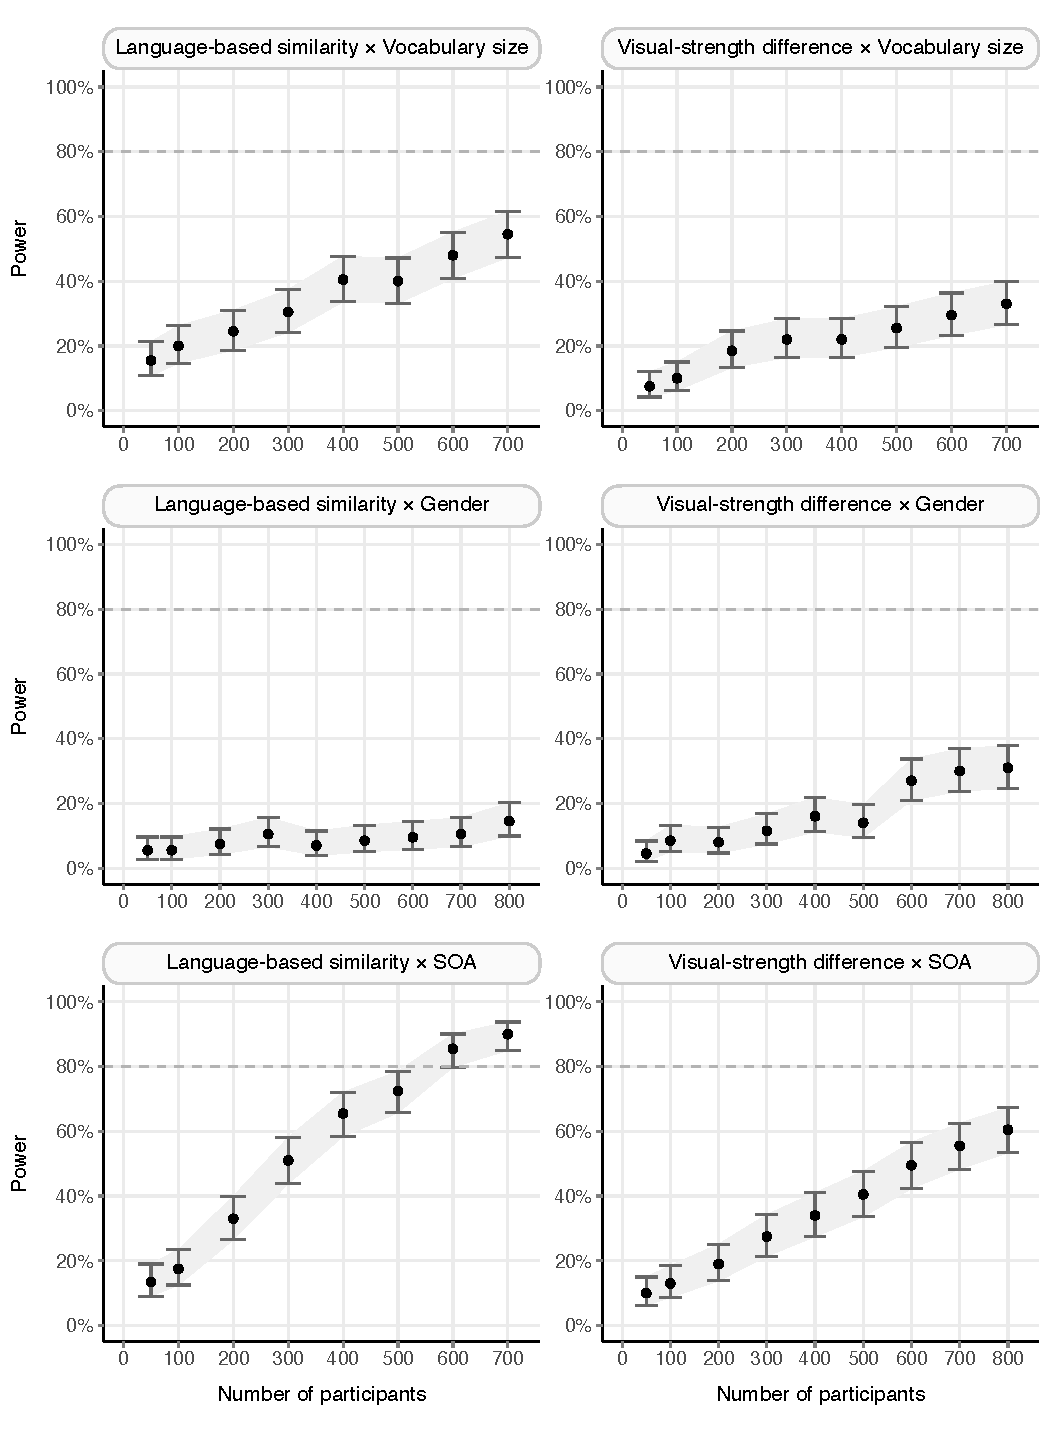
\includegraphics[width=0.92\linewidth]{C:/Users/Pablo/Documents/semanticpriming-semanticdecision-lexicaldecision/semanticpriming/power_analysis/plots/semanticpriming_powercurve_plots_4_5_6_7_8_9} 

}

\caption{Power curves for some interactions in the semantic priming study.}\label{fig:semanticpriming-powercurve-plots-4-5-6-7-8-9}
\end{figure}

\hypertarget{discussion-of-study-1}{%
\subsection{Discussion of Study 1}\label{discussion-of-study-1}}

The results revealed a significant, facilitatory effect of \texttt{language-based\ similarity} and a smaller but significant, inhibitory effect of \texttt{visual-strength\ difference}. That is, a greater language-based similarity resulted in shorter RTs, whereas a greater visual-strength difference resulted in larger RTs. There was also a sizable effect of stimulus onset asynchrony (SOA), with shorter RTs in the short SOA condition (200 ms) than in the long SOA (1,200 ms). Furthermore, there were significant interactions. First, language-based priming was larger in higher-vocabulary participants than in lower-vocabulary ones. Second, both language-based priming and vision-based priming were larger with the short SOA than with the long one. Thus far, these results broadly replicated those of Petilli et al. (2021). It is especially noteworthy that vision-based information had a significant effect, consistent with some of the previous research (Connell \& Lynott, 2014; Flores d'Arcais et al., 1985; Petilli et al., 2021; Schreuder et al., 1984), and contrasting with other research that did not find such an effect (Ostarek \& Huettig, 2017) or only observed it after visually-focussed tasks (Pecher et al., 1998; Yee et al., 2012). Last, no effect of gender was found. Below, we delve into some other aspects of these results.

\hypertarget{the-importance-of-outliers}{%
\subsubsection{The importance of outliers}\label{the-importance-of-outliers}}

The interaction between language-based similarity and vocabulary size (Figure \ref{fig:semanticpriming-interactions-with-vocabulary-size}-a) was patent in all deciles of vocabulary size but it was clearest among those participants that were more than one standard deviation away from the mean. Outliers in individual differences have played important roles in other areas of cognition as well, such as in the study of aphantasia and hyperphantasia---traits characterised, respectively, by a diminished and an extraordinary ability to mentally visualise objects (Milton et al., 2021; Zeman et al., 2020). Such an influence of outliers provides a reason to study more varied samples~of participants when possible. Furthermore, a greater interindividual variation might help detect the effects of individual differences that have been elusive (e.g., Hedge et al., 2018; Muraki \& Pexman, 2021; Ponari, Norbury, Rotaru, et al., 2018; Rodríguez-Ferreiro et al., 2020; Rouder \& Haaf, 2019).

\hypertarget{human-based-and-computational-measures-of-vision-based-information}{%
\subsubsection{Human-based and computational measures of vision-based information}\label{human-based-and-computational-measures-of-vision-based-information}}

Next, in a secondary analysis, we compared the roles of two measures of vision-based priming. The first measure---\texttt{visual-strength\ difference}---was operationalised as the difference in visual strength between the prime word and the target word in each trial. This difference score was thus based on modality-specific ratings provided by human participants (Lynott et al., 2020). The second measure---\texttt{vision-based\ similarity}---, created by Petilli et al. (2021), was based on vector representations trained on labelled images from ImageNet. This variable is therefore computational. The effect of visual-strength difference was slightly larger than that of vision-based similarity. This result is consistent with some previous findings suggesting that human-based measures explained more variance than computational measures (De Deyne et al., 2016, 2019; Gagné et al., 2016; Schmidtke et al., 2018; cf. Michaelov et al., 2022; Snefjella \& Blank, 2020). If the different degree of human dependence of our two variables were indeed behind the effect size of each, we would need to consider a related issue. The problem of circularity was addressed by Petilli et al., who argued that using human-based predictors---such as ratings---to investigate human behaviour was less valid than using predictors that were more independent of human behaviour---such as computational measures. On the one hand, we identify two reasons for skepticism regarding the circularity hypothesis. First, the underlying basis of all computational measures (e.g., Mandera et al., 2017; Petilli et al., 2021) is indeed human behaviour, notwithstanding the degree to which this human basis is filtered by computational methods. Second, we have not found sufficient research addressing the validity question. Yet, on the other hand, the circularity hypothesis is important enough to warrant dedicated research. Specifically, future studies could be conducted to systematically compare the theoretical insights provided by human-based measures and by computational ones, as well as the effect size achieved by both types.

It is noteworthy that both visual-strength difference and vision-based similarity have \emph{independently} proven to be relevant, and arguably valid, considering their correlations with other measures---especially \texttt{word-concreteness\ difference} and \texttt{language-based\ similarity}---and considering the effects of each measure in semantic priming (see Petilli et al., 2021). However, the differences between these measures are worthy of attention. Visual-strength difference was barely correlated with language-based similarity. Conversely, vision-based similarity was barely correlated with word-concreteness difference (refer to Figure \ref{fig:semanticpriming-with-visualsimilarity-correlations}). These results call for an investigation into the underlying composition of visual-strength difference and vision-based similarity.

Furthermore, whereas visual-strength difference retained its significant interaction with SOA---also observed in the main analysis presented above---, in contrast, vision-based similarity did not present such an interaction. The lack of an interaction between vision-based similarity and SOA contrasts with the results of Petilli et al. (2021), who found that vision-based similarity was only significant in the short SOA condition. There are several possible reasons for this difference, including: (I) a more conservative method in our current analysis---i.e., a maximal mixed-effects model containing more predictors than the hierarchical regression performed by Petilli et al.---, and (II) the presence of individual differences in the present study (i.e., vocabulary size, attentional control and gender), versus the aggregation performed by Petilli et al.

Last, the interaction between language-based similarity and SOA became non-significant in this sub-analysis. This difference from the original analysis may have been caused by the sizable correlation between language-based similarity and vision-based similarity (\(r\) = .49). In this regard, we should notice the large influence of the addition of a single variable (along with its interactions) into the model.

\hypertarget{the-influence-of-the-analytical-method}{%
\subsubsection{The influence of the analytical method}\label{the-influence-of-the-analytical-method}}

Taken together, the sub-analysis that included vision-based similarity offered a glimpse into the crucial role of analytical choices in the present topic. A previous example of this influence appeared in a set of studies that used Latent Semantic Analysis (LSA) as a predictor of semantic priming. Hutchison et al. (2008) operationalised LSA as a difference score, and did not find an effect of this variable. In contrast, later studies did not use a difference score and they observed a significant effect (Günther et al., 2016a; Mandera et al., 2017). We can extrapolate this issue to a very important comparison we often make---namely, that between language-based and embodied simulation. The pervasive superiority of language over the other systems (perception, action, emotion and sociality)---found in the three current studies and in previous ones (Banks et al., 2021; Kiela \& Bottou, 2014; Lam et al., 2015; Louwerse et al., 2015; Pecher et al., 1998; Petilli et al., 2021)---would be less trustworthy if the instruments that were used to measure the language system had been far more precise than the instruments used to measure the embodiment system. In this sense, it is relevant to consider how variables are improved in research: it is done iteratively, by comparing the performance of different variables. Critically, the literature contains many comparisons of text-based variables, some dating back to the 1990s (De Deyne et al., 2013, 2016; Günther et al., 2016a, 2016b; M. N. Jones et al., 2006; Lund \& Burgess, 1996; Mandera et al., 2017; Mikolov et al., 2013; Wingfield \& Connell, 2022a). In contrast, the work on embodiment variables began more than a decade afterwards, and it has been less concerned with benchmarking the explanatory power of variables (but see Vergallito et al., 2020). Instead, this literature contains more comparisons of different \emph{modalities}---e.g., visual strength, auditory strength, valence, etc. (Lynott et al., 2020; Lynott \& Connell, 2009; Newcombe et al., 2012). Thus, if linguistic measures are more precise than embodiment measures due to greater work on the variables, such a difference could account for a certain portion of the superiority of linguistic information over embodied information (see Banks et al., 2021; Kiela \& Bottou, 2014; Lam et al., 2015; Louwerse et al., 2015; Pecher et al., 1998; Petilli et al., 2021). Analytical choices such as the operationalisation of variables and the complexity of statistical models can greatly influence the conclusions of research. Indeed, our current results and previous ones suggest that the conclusions of research are inextricable from the method used in each study (see Barsalou, 2019; Botvinik-Nezer et al., 2020; Perret \& Bonin, 2019; Wagenmakers et al., 2022). Therefore, in the medium term, it may pay dividends to continue examining the influence of analytical choices. Unfortunately, in many research fields, reflecting on the sensitivity of our analyses might conflict with the incentives of the system, which may penalise nuanced conclusions in favour of simplified stories. To overcome such a bias, it may be necessary to devote greater importance to the methodology in scientific papers---for instance, by commenting on the method in the abstract and by extending the methods section in the body of the paper. In stark contrast, our current results should make us question some decisions by scientific publishers such as rendering the methods section in a smaller font than the results section, or placing the method section at the end of the paper. In a nutshell, it may be useful to ensure that scientists are aware that research findings are fundamentally dependent on research methods.

\hypertarget{statistical-power-analysis-3}{%
\subsubsection{Statistical power analysis}\label{statistical-power-analysis-3}}

We analysed the statistical power associated with several effects of interest, across various sample sizes. The results of this power analysis can help determine the number of participants required to reliably examine each of these effects in a future study. Importantly, the results assume two conditions. First, the future study would apply a statistical method similar to ours---namely, a mixed-effects model with random intercepts and slopes. Second, the analysis of the future study would encompass at least 5,943 prime--target pairs (distributed in various blocks across participants, not all being presented to every participant).

First, the results revealed that detecting the main effect of language-based similarity would require 50 participants. Next, detecting the interaction between language-based similarity and SOA would require 600 participants. Last, the other effects would require more than 1,000 participants---or, in the case of gender differences, many more than that.

\clearpage

\hypertarget{study-2-semantic-decision}{%
\section{Study 2: Semantic decision}\label{study-2-semantic-decision}}

The semantic decision task probes the role of concreteness in conceptual processing. Specifically, this task requires participants to classify words as abstract or concrete, which elicits deeper semantic processing than the task of identifying word forms (i.e., lexical decision). Researchers then analyse whether the responses can be explained by the sensory experientiality of the referents---that is, the degree to which they can be experienced through our senses---and by other variables, such as word frequency. The core data set in this study was that of the Calgary Semantic Decision Project (Pexman et al., 2017; Pexman \& Yap, 2018). The experimental task is semantic decision, in which participants judge whether words are primarily abstract (e.g., \emph{thought}) or concrete (e.g., \emph{building}).

Research has found that the processing of relatively concrete words relies considerably on sensorimotor information (Hultén et al., 2021; Kousta et al., 2011; Vigliocco et al., 2014). In contrast, the processing of relatively abstract words seems to draw more heavily on information from language (Barca et al., 2020; Duñabeitia et al., 2009; Snefjella \& Blank, 2020), emotion (Kousta et al., 2011; Ponari et al., 2020; Ponari, Norbury, Rotaru, et al., 2018; Ponari, Norbury, \& Vigliocco, 2018; Vigliocco et al., 2014), interoception (Connell et al., 2018) and social information (Borghi et al., 2022, 2019; Diveica et al., 2022).

\hypertarget{methods-1}{%
\subsection{Methods}\label{methods-1}}

\hypertarget{data-set}{%
\subsubsection{Data set}\label{data-set}}

The data set was trimmed by removing rows that lacked values on any variable, and by also removing RTs that were more than 3 standard deviations away from the mean.\footnote{In the removal of missing values, six participants whose gender appeared as `NA' were inadvertently removed from the data set.} The standard deviation trimming was performed within participants and within trial blocks, as done in the Calgary Semantic Decision Project (Pexman et al., 2017). The resulting data set contained 306 participants, 8,927 words and 246,432 RTs. On average, there were 755 words per participant (\(SD\) = 42.05), and conversely, 26 participants per word (\(SD\) = 4.80).

\hypertarget{variables-1}{%
\subsubsection{Variables}\label{variables-1}}

While the variables are generally described in the \protect\hyperlink{present-studies}{\underline{general introduction}}, a few further details are provided below regarding some of them.

\hypertarget{vocabulary-size}{%
\paragraph{Vocabulary size}\label{vocabulary-size}}

In the vocabulary test used by Pexman et al. (2017), participants were presented with 35 rare words with irregular pronunciations (e.g., \emph{gaoled}, \emph{ennui}), and they were asked to read the words aloud (also see Pexman \& Yap, 2018). When they pronounced a word correctly, it was inferred that they knew the word. This test was based on NAART35, a short version of the North American Adult Reading Test (Uttl, 2002).

\hypertarget{word-co-occurrence}{%
\paragraph{Word co-occurrence}\label{word-co-occurrence}}

Wingfield and Connell (2022a) reanalysed the data from Pexman et al. (2017) using language-based variables that are more related to the language system than to the visual system. The task used by Pexman et al.~was semantic decision, in which participants assessed whether words were abstract or concrete. Wingfield and Connell found that the variables that best explained RTs were word co-occurrence measures. Specifically, one of these variables was the corpus distance between each stimulus word and the word `abstract'. The other variable was the corpus distance between each stimulus word and the word `concrete'. Wingfield and Connell studied these distance measures in various forms, and found that cosine and correlation distance yielded the best results. We used the correlation distances following the advice of Kiela and Bottou (2014).

The zero-order correlation between Wingfield and Connell's (2022) distance to `abstract' and distance to `concrete' was \(r\) = .98. To avoid the collinearity between these variables in the model (Dormann et al., 2013; Harrison et al., 2018), and to facilitate the analysis of interactions with other variables, we created a difference score by subtracting the distance to `abstract' from the distance to `concrete'. This new variable was named `word co-occurrence'. As shown in Figure \ref{fig:semanticdecision-cooccurrence-correlations}, the correlation between word co-occurrence and word concreteness was twice as large as the correlation between either form of the distance and word concreteness. This suggested that the difference score had successfully encapsulated the information of both distances.

\begin{figure}

{\centering 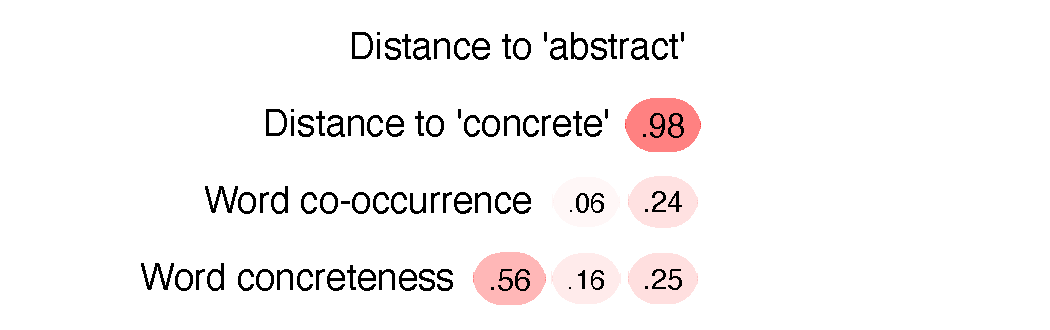
\includegraphics[width=0.63\linewidth]{manuscript_files/figure-latex/semanticdecision-cooccurrence-correlations-1} 

}

\caption{Zero-order correlations among Wingfield and Connell's (2022) distances, the difference score (word co-occurrence) and word concreteness (Brysbaert et al., 2014).}\label{fig:semanticdecision-cooccurrence-correlations}
\end{figure}

A few details regarding the covariates follow.

\begin{itemize}
\item
  \texttt{Information\ uptake} was included as a measure akin to general cognition, and specifically as a covariate of vocabulary size (Ratcliff et al., 2010; also see James et al., 2018; Pexman \& Yap, 2018). Information uptake was effectively the drift rate per participant in Pexman and Yap (2018). This drift rate measured participants' ability to correctly and quickly perform the semantic decision task, in which they classified words as abstract or concrete (for graphical illustrations, see Lerche et al., 2020; van Ravenzwaaij et al., 2012). In other words, drift rate measures an individual's ability (Lerche et al., 2020; Pexman \& Yap, 2018).
\item
  Lexical covariates (see \protect\hyperlink{appendix-A-lexical-covariates}{\underline{Appendix A}}): \texttt{word\ frequency} and \texttt{orthographic\ Levenshtein\ distance} (Balota et al., 2007).
\item
  \texttt{Word\ concreteness} (Brysbaert et al., 2014): a fundamental variable in the semantic decision task, in which participants judge whether words are abstract or concrete (for further considerations, see Bottini et al., 2021). Indeed, owing to the instructions of the task, word concreteness is likely to be more relevant to the participants' task than our effects of interest.
\end{itemize}

Figure \ref{fig:semanticdecision-correlations} shows the correlations among the predictors and the dependent variable.

\begin{figure}

{\centering 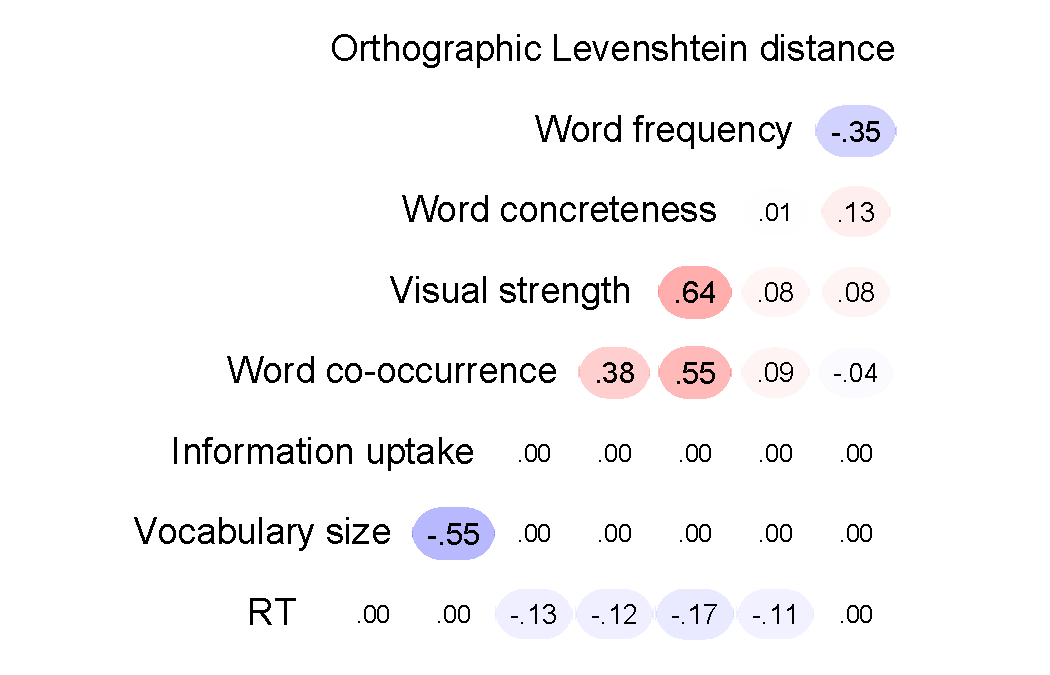
\includegraphics[width=0.61\linewidth]{manuscript_files/figure-latex/semanticdecision-correlations-1} 

}

\caption{Zero-order correlations in the semantic decision study.}\label{fig:semanticdecision-correlations}
\end{figure}

\hypertarget{diagnostics-for-the-frequentist-analysis-2}{%
\subsubsection{Diagnostics for the frequentist analysis}\label{diagnostics-for-the-frequentist-analysis-2}}

The model presented convergence warnings. To avoid removing important random slopes, which could increase the Type I error rate---i.e., false positives (Brauer \& Curtin, 2018; Singmann \& Kellen, 2019), we examined the model after refitting it using seven optimisation algorithms through the `allFit' function of the `lme4' package (Bates et al., 2021). The results showed that all optimisers produced virtually identical means for all effects, suggesting that the convergence warnings were not consequential (Bates et al., 2021; see \protect\hyperlink{appendix-B-frequentist-analysis-diagnostics}{\underline{Appendix B}}).

The residual errors were not normally distributed, and attempts to mitigate this deviation proved unsuccessful (see \protect\hyperlink{appendix-B-frequentist-analysis-diagnostics}{\underline{Appendix B}}). However, this is not likely to have posed a major problem, as mixed-effects models are fairly robust to deviations from normality (Knief \& Forstmeier, 2021; Schielzeth et al., 2020). Last, the model did not present multicollinearity problems, with all VIFs below 2 (see Dormann et al., 2013; Harrison et al., 2018).

\hypertarget{diagnostics-for-the-bayesian-analysis-1}{%
\subsubsection{Diagnostics for the Bayesian analysis}\label{diagnostics-for-the-bayesian-analysis-1}}

Three Bayesian models were run that were respectively characterised by informative, weakly-informative and diffuse priors. In each model, 16 chains were used. In each chain, 2,000 warmup iterations were run, followed by 6,000 post-warmup iterations. Thus, a total of 96,000 post-warmup draws were produced over all the chains.

The maximum \(\widehat R\) value for the fixed effects across the three models was 1.42, far exceeding the 1.01 threshold (Vehtari et al., 2021; also see Schoot et al., 2021). Similarly, the maximum \(\widehat R\) value for the random effects was 1.31. Furthermore, the posterior predictive checks revealed major divergences between the observed data and the posterior distributions (see \protect\hyperlink{appendix-C-Bayesian-analysis-diagnostics}{\underline{Appendix C}}). In conclusion, since the Bayesian results were not valid, they are not shown in the main text, but are available in \protect\hyperlink{appendix-E-Bayesian-analysis-results}{\underline{Appendix E}}.

\hypertarget{results-of-study-2}{%
\subsection{Results of Study 2}\label{results-of-study-2}}

Table \ref{tab:semanticdecision-frequentist-model} presents the results. The fixed effects explained 4.11\% of the variance, and the random effects explained 17.48\% (Nakagawa et al., 2017; for an explanation of this difference, see \protect\hyperlink{semanticpriming-results}{\underline{Results of Study 1}}). Both word co-occurrence and visual strength produced significant main effects. Higher values of these variables facilitated participants' performance, as reflected in shorter RTs. Furthermore, visual strength interacted with vocabulary size. There were no effects of participants' gender (see interaction figures below).

The effect sizes of word co-occurrence and its interactions were larger than those of visual strength. Figure \ref{fig:semanticdecision-confidence-intervals-plot} displays these estimates.\footnote{Only frequentist estimates shown, as Bayesian ones were not valid (see \protect\hyperlink{appendix-E-Bayesian-analysis-results}{\underline{Appendix E}}).}

\begin{table}[!h]

\caption{\label{tab:semanticdecision-frequentist-model}Frequentist model for the semantic decision study.}
\centering
\begin{threeparttable}
\begin{tabular}[t]{lrrrrr}
\toprule
\multicolumn{1}{c}{ } & \multicolumn{1}{c}{$\upbeta$} & \multicolumn{1}{c}{$SE$} & \multicolumn{1}{c}{95\% CI} & \multicolumn{1}{c}{$t$} & \multicolumn{1}{c}{$p$}\\
\midrule
(Intercept) & 0.05 & 0.00 & {}[0.04, 0.06] & 11.87 & <.001\\
\addlinespace[0.3em]
\multicolumn{6}{l}{\textbf{Individual differences}}\\
\cellcolor{gray!6}{\hspace{1em}Information uptake} & \cellcolor{gray!6}{0.00} & \cellcolor{gray!6}{0.00} & \cellcolor{gray!6}{{}[0.00, 0.00]} & \cellcolor{gray!6}{0.20} & \cellcolor{gray!6}{.844}\\
\hspace{1em}Vocabulary size $^{\text{a}}$ & 0.00 & 0.00 & {}[-0.01, 0.00] & -1.42 & .155\\
\hspace{1em}Gender $^{\text{a}}$ & 0.00 & 0.00 & {}[0.00, 0.00] & -0.47 & .636\\
\addlinespace[0.3em]
\multicolumn{6}{l}{\textbf{Lexicosemantic covariates}}\\
\cellcolor{gray!6}{\hspace{1em}Word frequency} & \cellcolor{gray!6}{-0.12} & \cellcolor{gray!6}{0.00} & \cellcolor{gray!6}{{}[-0.13, -0.12]} & \cellcolor{gray!6}{-28.63} & \cellcolor{gray!6}{<.001}\\
\cellcolor{gray!6}{\hspace{1em}Orthographic Levenshtein distance} & \cellcolor{gray!6}{-0.01} & \cellcolor{gray!6}{0.00} & \cellcolor{gray!6}{{}[-0.02, 0.00]} & \cellcolor{gray!6}{-3.05} & \cellcolor{gray!6}{.002}\\
\cellcolor{gray!6}{\hspace{1em}Word concreteness} & \cellcolor{gray!6}{-0.13} & \cellcolor{gray!6}{0.01} & \cellcolor{gray!6}{{}[-0.14, -0.11]} & \cellcolor{gray!6}{-21.39} & \cellcolor{gray!6}{<.001}\\
\addlinespace[0.3em]
\multicolumn{6}{l}{\textbf{Semantic variables}}\\
\hspace{1em}Word co-occurrence $^{\text{b}}$ & -0.03 & 0.01 & {}[-0.04, -0.02] & -4.48 & <.001\\
\hspace{1em}Visual strength $^{\text{b}}$ & -0.02 & 0.01 & {}[-0.03, -0.01] & -2.91 & .004\\
\addlinespace[0.3em]
\multicolumn{6}{l}{\textbf{Interactions}}\\
\cellcolor{gray!6}{\hspace{1em}Word concreteness  $\times$  Vocabulary size} & \cellcolor{gray!6}{-0.02} & \cellcolor{gray!6}{0.00} & \cellcolor{gray!6}{{}[-0.03, -0.02]} & \cellcolor{gray!6}{-7.66} & \cellcolor{gray!6}{<.001}\\
\cellcolor{gray!6}{\hspace{1em}Word concreteness  $\times$  Gender} & \cellcolor{gray!6}{-0.01} & \cellcolor{gray!6}{0.00} & \cellcolor{gray!6}{{}[-0.02, 0.00]} & \cellcolor{gray!6}{-3.50} & \cellcolor{gray!6}{<.001}\\
\cellcolor{gray!6}{\hspace{1em}Word co-occurrence  $\times$  Information uptake} & \cellcolor{gray!6}{0.01} & \cellcolor{gray!6}{0.01} & \cellcolor{gray!6}{{}[0.00, 0.02]} & \cellcolor{gray!6}{1.48} & \cellcolor{gray!6}{.141}\\
\cellcolor{gray!6}{\hspace{1em}Visual strength  $\times$  Information uptake} & \cellcolor{gray!6}{0.02} & \cellcolor{gray!6}{0.01} & \cellcolor{gray!6}{{}[0.01, 0.03]} & \cellcolor{gray!6}{3.05} & \cellcolor{gray!6}{.003}\\
\hspace{1em}Word co-occurrence  $\times$  Vocabulary size & 0.01 & 0.01 & {}[0.00, 0.02] & 1.66 & .098\\
\hspace{1em}Visual strength  $\times$  Vocabulary size & 0.01 & 0.01 & {}[0.00, 0.02] & 2.03 & .043\\
\hspace{1em}Word co-occurrence  $\times$  Gender & 0.00 & 0.00 & {}[-0.01, 0.01] & 0.86 & .393\\
\hspace{1em}Visual strength  $\times$  Gender & 0.00 & 0.00 & {}[-0.01, 0.01] & -0.08 & .940\\
\bottomrule
\end{tabular}
\begin{tablenotes}
\item \textit{\linebreak} 
\item \textit{Note}. $\upbeta$ = Estimate based on $z$-scored predictors; \textit{SE} = standard error; \linebreak \phantom{.}CI = confidence interval. Shaded rows contain covariates. \linebreak \linebreak \phantom{.}$^{\text{a}}$ By-word random slopes were included for this effect. \linebreak \phantom{.}$^{\text{b}}$ By-participant random slopes were included for this effect.
\end{tablenotes}
\end{threeparttable}
\end{table}

\FloatBarrier

\begin{figure}

{\centering 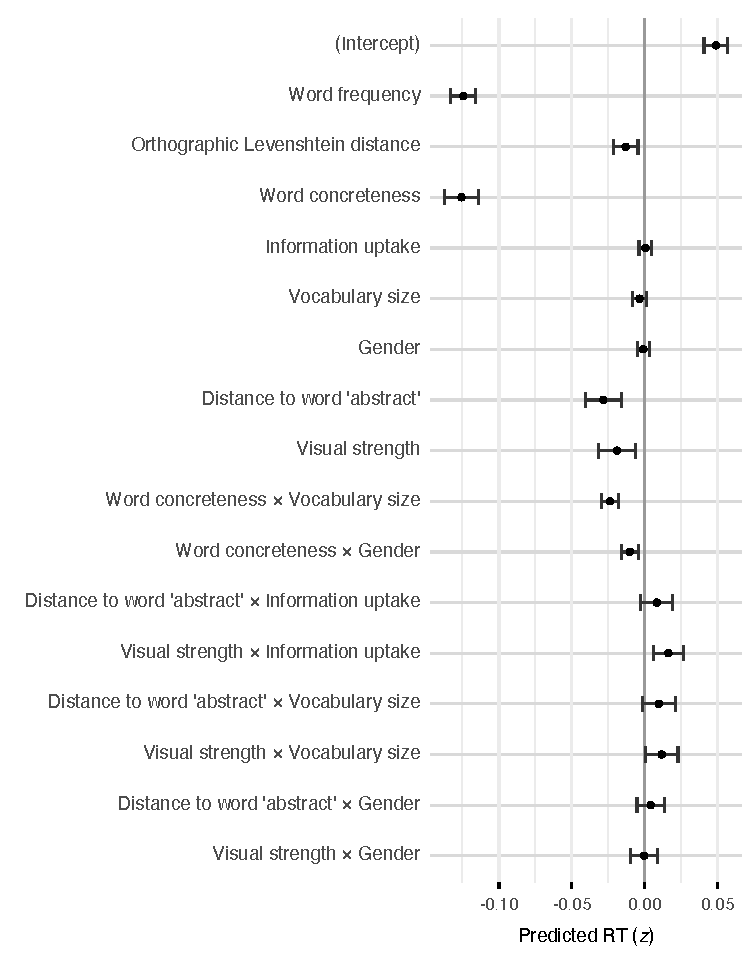
\includegraphics[width=1\linewidth]{C:/Users/Pablo/Documents/semanticpriming-semanticdecision-lexicaldecision/semanticdecision/frequentist_analysis/plots/semanticdecision_confidence_intervals_plot} 

}

\caption{Means and 95\% confidence intervals for the effects of interest in the semantic decision study.}\label{fig:semanticdecision-confidence-intervals-plot}
\end{figure}

Figure \ref{fig:semanticdecision-interactions-with-vocabulary-size}-a shows the non-significant interaction between word co-occurrence and vocabulary size, whereby lower-vocabulary participants were more sensitive to word co-occurrence than higher-vocabulary participants. Next, Figure \ref{fig:semanticdecision-interactions-with-vocabulary-size}-b shows the significant interaction between visual strength and vocabulary size, demonstrating that lower-vocabulary participants were also more sensitive to visual strength. Last, Figure \ref{fig:semanticdecision-interactions-with-vocabulary-size}-c shows the significant interaction between word concreteness and vocabulary size, whereby higher-vocabulary participants were more sensitive to word concreteness than lower-vocabulary participants. Word concreteness is likely the most relevant variable for the semantic decision task, in which participants classify words as abstract or concrete. In conclusion, these interactions suggest that higher-vocabulary participants were better able to focus on the most relevant information, whereas lower-vocabulary participants were
sensitive to a greater breadth of information (see Lim et al., 2020; Pexman \& Yap, 2018; Yap et al., 2009, 2012, 2017).



\begin{figure}

{\centering 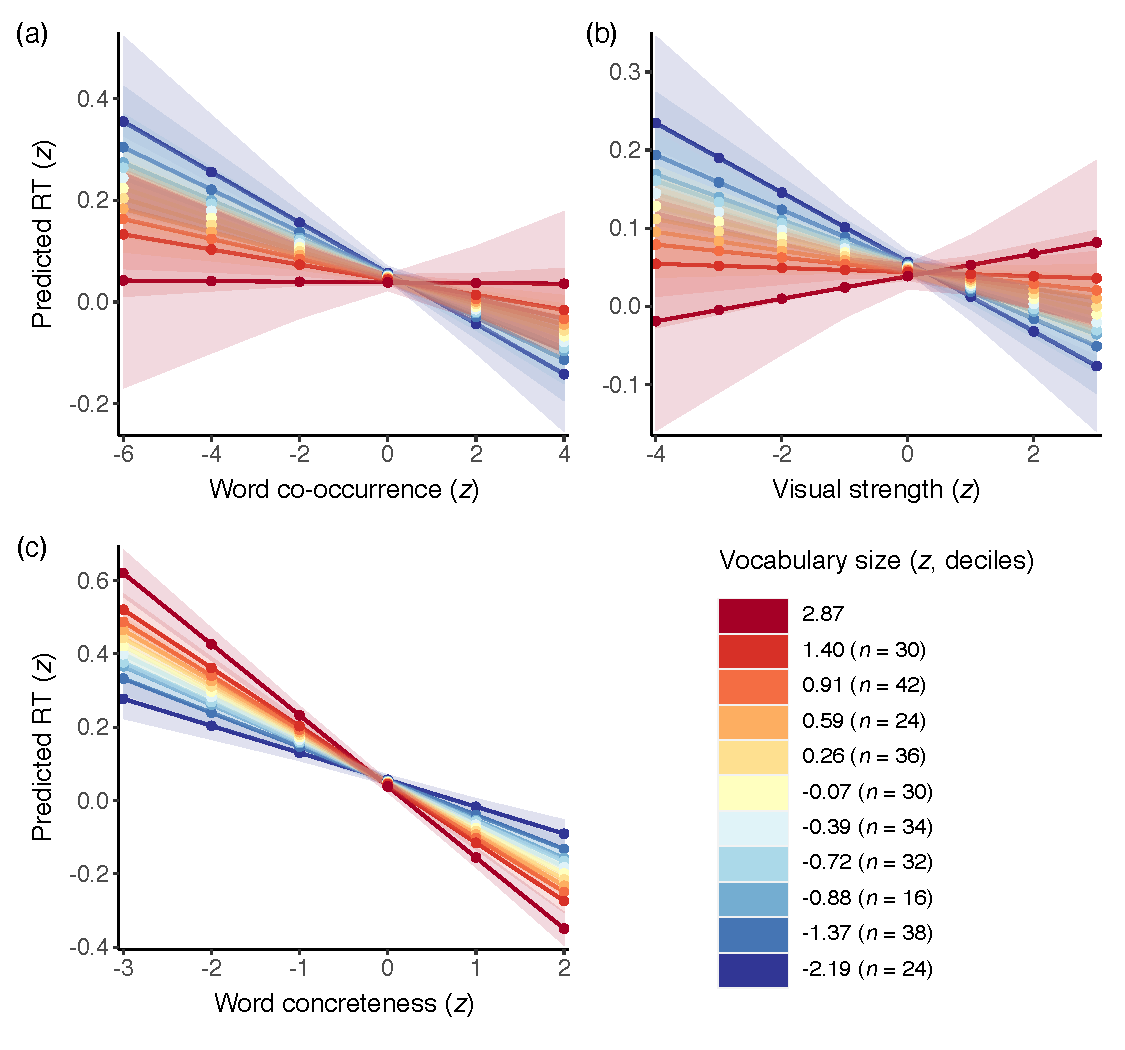
\includegraphics[width=0.98\linewidth]{C:/Users/Pablo/Documents/semanticpriming-semanticdecision-lexicaldecision/semanticdecision/frequentist_analysis/plots/semanticdecision-interactions-with-vocabulary-size} 

}

\caption{Interactions of vocabulary size with language-based information (panel a), with visual strength (panel b) and with word concreteness (panel c) in the semantic decision study. Vocabulary size is constrained to deciles in this plot, whereas in the statistical analysis it contained more values within the current range. \(n\) = number of participants contained between deciles.}\label{fig:semanticdecision-interactions-with-vocabulary-size}
\end{figure}

A continuous measure of word concreteness was used in the present study. In contrast, Pexman and Yap (2018) split the data set it into a subset with abstract words and another subset with concrete words, and they analysed these subsets separately. Pexman and Yap found that high-vocabulary participants were more sensitive to the relative abstractness of words. Specifically, these participants were faster to classify very abstract words than mid-abstract ones, thus presenting a reverse concreteness effect (also see Bonner et al., 2009). Such a reverse effect might stem from the bimodal distributions that have appeared in concreteness ratings (Brysbaert et al., 2014) and in semantic decisions (Pexman \& Yap, 2018), or it might be due to confounding variables (Hoffman \& Lambon Ralph, 2011). Notwithstanding the bimodal distributions, Troche et al. (2017) suggested that a continuous analysis remained necessary to study word concreteness (also see Cohen, 1983). Consistent with this, our present findings demonstrated the sensitivity of a continuous word concreteness variable to patterns such as the greater role of task-relevant variables in high-vocabulary participants. In conclusion, the literature and our findings suggest that the split-data approach and the continuous approach to word concreteness are both useful. Where it is feasible, the application of both approaches would provide the greatest information.

Figure \ref{fig:semanticdecision-interactions-with-gender} shows the interactions with gender. The interactions of interest, in panels a and b, were non-significant.\footnote{Further interaction plots available in \protect\hyperlink{appendix-D-interaction-plots}{\underline{Appendix D}}.}

\begin{figure}

{\centering 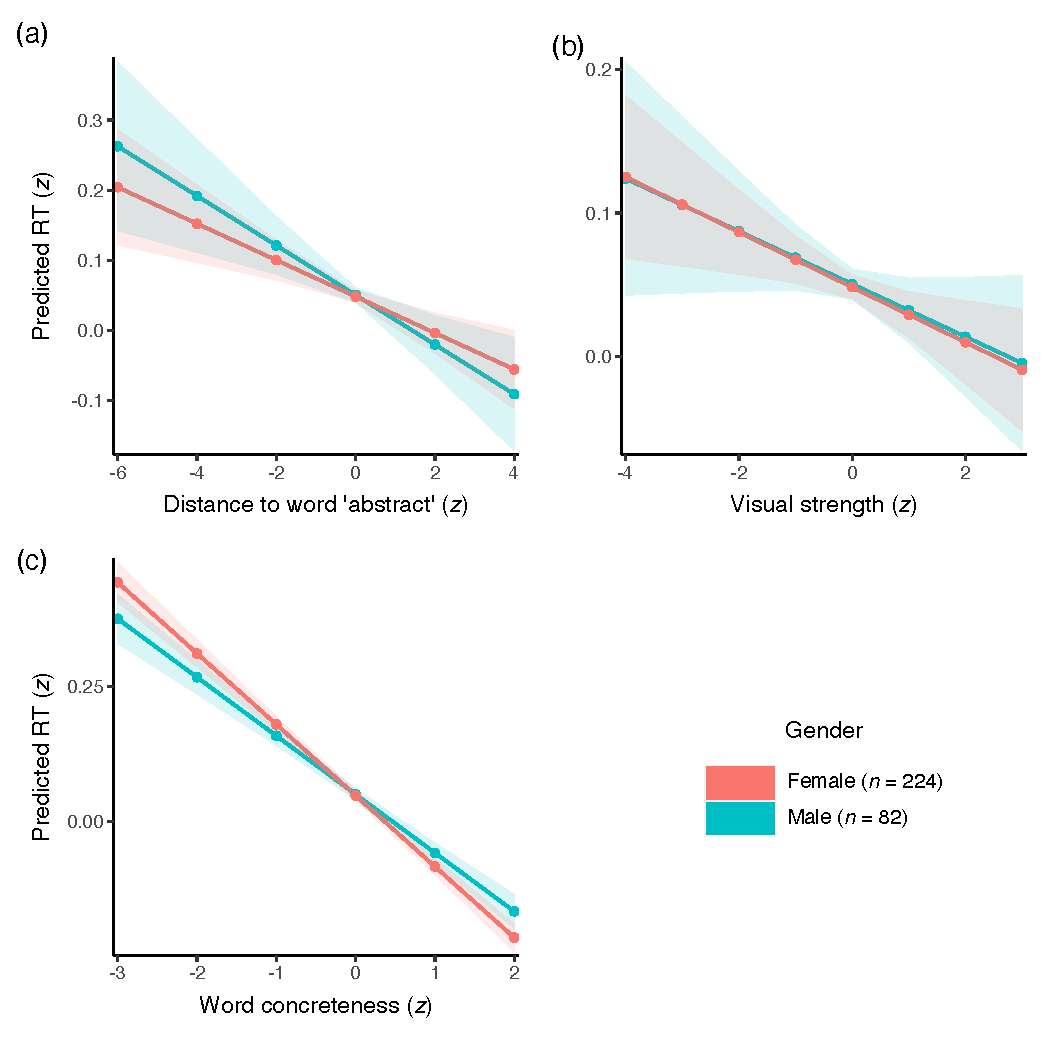
\includegraphics[width=0.98\linewidth]{C:/Users/Pablo/Documents/semanticpriming-semanticdecision-lexicaldecision/semanticdecision/frequentist_analysis/plots/semanticdecision-interactions-with-gender} 

}

\caption{Interactions of gender with word co-occurrence (panel a), with visual strength (panel b) and with word concreteness (panel c) in the semantic decision study. Gender was analysed using $z$-scores, but for clarity, the basic labels are used in the legend.}\label{fig:semanticdecision-interactions-with-gender}
\end{figure}

\hypertarget{statistical-power-analysis-4}{%
\subsubsection{Statistical power analysis}\label{statistical-power-analysis-4}}

Figures \ref{fig:semanticdecision-powercurve-plots-1-2-3} and \ref{fig:semanticdecision-powercurve-plots-4-5-6-7} show the estimated power for some main effects and interactions of interest as a function of the number of participants. To plan the sample size for future studies, these results must be considered under the assumptions that the future study would apply a statistical method similar to ours---namely, a mixed-effects model with random intercepts and slopes---, and that the analysis would encompass at least as many words as the current study, namely, 8,927 (distributed in various blocks across participants, not all being presented to every participant). Furthermore, it is necessary to consider each figure in detail. Here, we provide a summary. First, detecting the main effect of word co-occurrence would require 300 participants. Second, detecting the main effect of visual strength would require 1,200 participants. Third, detecting the interactions of word co-occurrence and visual strength with vocabulary size would require 1,500 participants. Last, detecting the other effects would require more than 2,000 participants---or, in the case of gender differences, many more than that.

\begin{figure}

{\centering 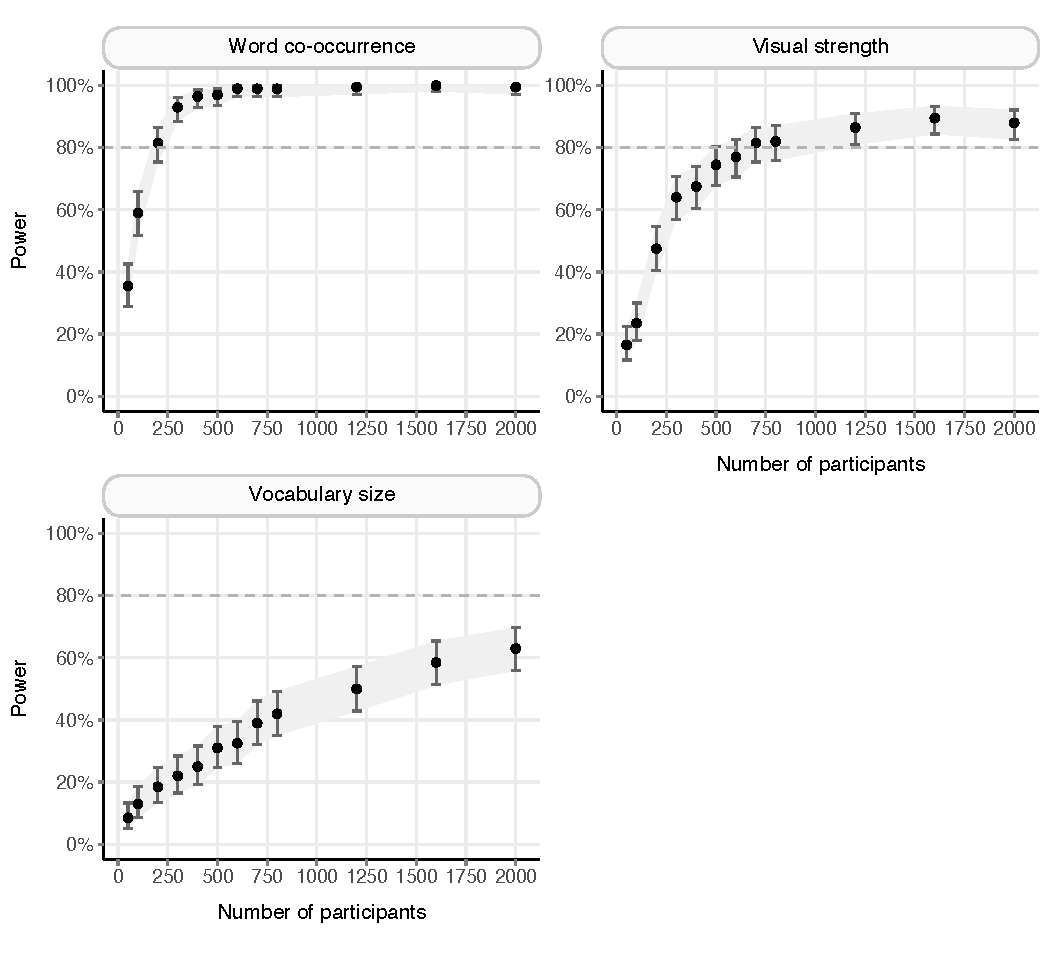
\includegraphics[width=1\linewidth]{C:/Users/Pablo/Documents/semanticpriming-semanticdecision-lexicaldecision/semanticdecision/power_analysis/plots/semanticdecision_powercurve_plots_1_2_3} 

}

\caption{Power curves for some main effects in the semantic decision study.}\label{fig:semanticdecision-powercurve-plots-1-2-3}
\end{figure}

\begin{figure}

{\centering 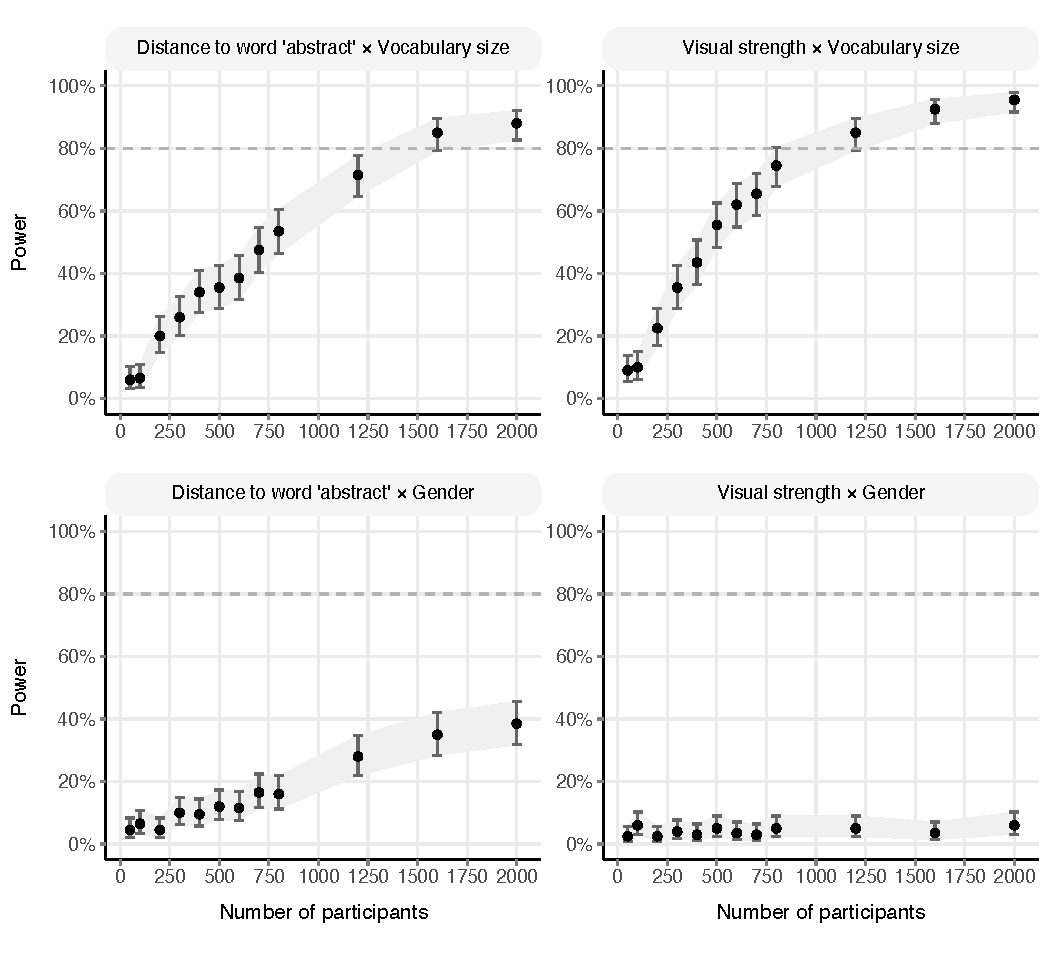
\includegraphics[width=1\linewidth]{C:/Users/Pablo/Documents/semanticpriming-semanticdecision-lexicaldecision/semanticdecision/power_analysis/plots/semanticdecision_powercurve_plots_4_5_6_7} 

}

\caption{Power curves for some interactions in the semantic decision study.}\label{fig:semanticdecision-powercurve-plots-4-5-6-7}
\end{figure}

\hypertarget{discussion-of-study-2}{%
\subsection{Discussion of Study 2}\label{discussion-of-study-2}}

The results revealed a significant, facilitatory effect of \texttt{word\ co-occurrence} and a smaller but significant, facilitatory effect of \texttt{visual\ strength}. That is, higher values of these variables resulted in shorter RTs. Furthermore, there were significant interactions. First, language-based priming was larger in higher-vocabulary participants than in lower-vocabulary ones. Second, both language-based priming and vision-based priming were larger with the short SOA than with the long one. Thus far, these results broadly replicated those of Petilli et al. (2021). As in Study 1, vision-based information had a significant effect. This was to be expected, as semantic decision is likely to engage deeper semantic processing. Last, no effect of gender was found. Below, we delve into some other aspects of these results.

\hypertarget{statistical-power-analysis-5}{%
\subsubsection{Statistical power analysis}\label{statistical-power-analysis-5}}

We analysed the statistical power associated with several effects of interest, across various sample sizes. The results of this power analysis can help determine the number of participants required to reliably examine each of these effects in a future study. Importantly, the results assume two conditions. First, the future study would apply a statistical method similar to ours---namely, a mixed-effects model with random intercepts and slopes. Second, the analysis of the future study would encompass at least 8,927 stimulus words (distributed in various blocks across participants, not all being presented to every participant).

First, the results revealed that detecting the main effect of word co-occurrence would require 300 participants. Next, detecting the interactions with vocabulary size would require 1,500 participants. Last, detecting the other effects would require more than 2,000 participants---or, in the case of gender differences, many more than that.

\clearpage

\hypertarget{lexicaldecision}{%
\section{Study 3: Lexical decision}\label{lexicaldecision}}

The core data set in this study was the lexical decision subset of the English Lexicon Project (ELP; Balota et al., 2007). As in Study 1, we limited our analysis to the lexical decision task because it was more relevant to a subsequent study that we were planning. The lexical decision task differs from semantic priming and semantic decision in two important aspects. First, lexical decision is likely to involve less semantic processing than the other paradigms (Balota \& Lorch, 1986; Becker et al., 1997; de Wit \& Kinoshita, 2015; Joordens \& Becker, 1997; Muraki \& Pexman, 2021; Ostarek \& Huettig, 2017).

Second, it is more difficult in the lexical decision task to create word-to-word distance measures to capture language-based and vision-based information. The possibility of calculating the distance between words in consecutive trials is hindered by the need to skip trials, owing to the high prevalence of nonword trials throughout the lexical decision task. Therefore, the measures must be based on each word alone. Accordingly, vision-based information can be operationalised as the visual strength of each word. Language-based information could be operationalised as one of several lexical variables. In the present study, word frequency was chosen as it had the largest effect size out of five candidates---the other candidates being number of letters, number of syllables, orthographic Levenshtein distance and phonological Levenshtein distance (see \protect\hyperlink{appendix-A-lexical-covariates}{\underline{Appendix A}}). It should also be noted that word frequency has been found to be more closely related to semantic variables than to lexical ones, such as word length, orthography and phonology (see Table 4 in Yap et al., 2012). Another noteworthy feature of word frequency how it relates to vocabulary size across different paradigms. In lexical decision, the effect of word frequency has been stronger in higher-vocabulary participants than in lower-vocabulary ones (Lim et al., 2020; Yap et al., 2012). In contrast, the opposite pattern has emerged in deeper semantic tasks, such as semantic priming (Yap et al., 2017) and semantic decision (Pexman \& Yap, 2018).

\hypertarget{methods-2}{%
\subsection{Methods}\label{methods-2}}

\hypertarget{data-set-1}{%
\subsubsection{Data set}\label{data-set-1}}

The data set was trimmed by removing rows that lacked values on any variable, and by also removing RTs that were more than 3 standard deviations away from the mean. The standard deviation trimming was performed within participants, as done in the English Lexicon Project (Balota et al., 2007). The resulting data set contained 795 participants, 12,636 words and 19,828 RTs. On average, there were 25 words per participant (\(SD\) = 36.04), and conversely, 2 participants per word (\(SD\) = 0.86).

Figure \ref{fig:lexicaldecision-correlations} shows the correlations among the predictors and the dependent variable.

\begin{figure}

{\centering 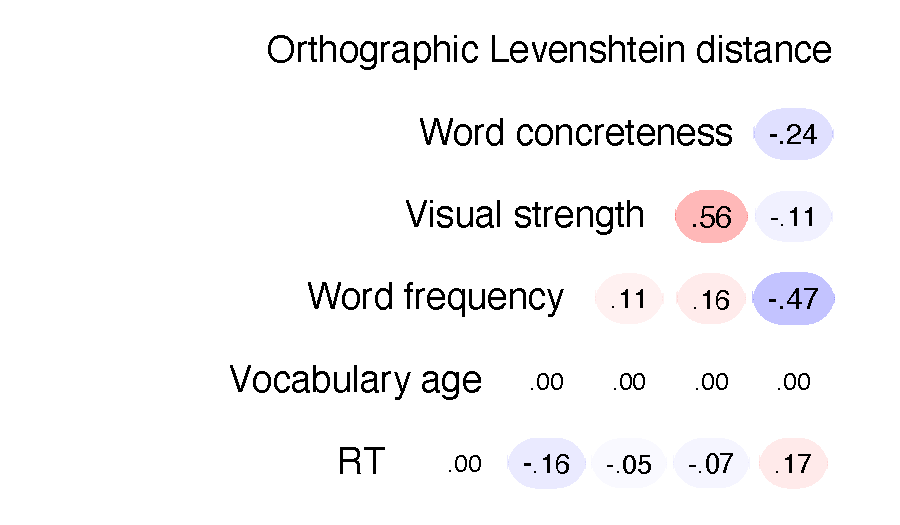
\includegraphics[width=0.52\linewidth]{manuscript_files/figure-latex/lexicaldecision-correlations-1} 

}

\caption{Zero-order correlations in the lexical decision study.}\label{fig:lexicaldecision-correlations}
\end{figure}

\hypertarget{variables-2}{%
\subsubsection{Variables}\label{variables-2}}

While the variables are generally described in the \protect\hyperlink{present-studies}{\underline{general introduction}}, a few further details are provided below regarding some of them.

\begin{itemize}
\tightlist
\item
  \texttt{Vocabulary\ age}: the present study uses the name vocabulary \emph{age}, as used in the study of Balota et al. (2007). It measures the same linguistic experience as vocabulary size.
\end{itemize}

A few details regarding the covariates follow.

\begin{itemize}
\item
  General cognition covariate: unlike in the two previous studies, the present study did not include a general cognition covariate as such a variable was not available in the data set of Balota et al. (2007).
\item
  Lexical covariates (see preselection in \protect\hyperlink{appendix-A-lexical-covariates}{\underline{Appendix A}}): \texttt{orthographic\ Levenshtein\ distance} (Balota et al., 2007).
\item
  \texttt{Word\ concreteness} (Brysbaert et al., 2014), used as a covariate of visual strength.
\end{itemize}

\hypertarget{diagnostics-for-the-frequentist-analysis-3}{%
\subsubsection{Diagnostics for the frequentist analysis}\label{diagnostics-for-the-frequentist-analysis-3}}

The model presented convergence warnings. To avoid removing important random slopes, which could increase the Type I error rate---i.e., false positives (Brauer \& Curtin, 2018; Singmann \& Kellen, 2019), we examined the model after refitting it using seven optimisation algorithms through the `allFit' function of the `lme4' package (Bates et al., 2021). The results showed that all optimisers produced virtually identical means for all effects, suggesting that the convergence warnings were not consequential (Bates et al., 2021; see \protect\hyperlink{appendix-B-frequentist-analysis-diagnostics}{\underline{Appendix B}}).

The residual errors were not normally distributed, and attempts to mitigate this deviation proved unsuccessful (see \protect\hyperlink{appendix-B-frequentist-analysis-diagnostics}{\underline{Appendix B}}). However, this is not likely to have posed a major problem, as mixed-effects models are fairly robust to deviations from normality (Knief \& Forstmeier, 2021; Schielzeth et al., 2020). Last, the model did not present multicollinearity problems, with all VIFs below 2 (see Dormann et al., 2013; Harrison et al., 2018).

\hypertarget{diagnostics-for-the-bayesian-analysis-2}{%
\subsubsection{Diagnostics for the Bayesian analysis}\label{diagnostics-for-the-bayesian-analysis-2}}

Three Bayesian models were run that were respectively characterised by informative, weakly-informative and diffuse priors. In each model, 5 chains were used. In each chain, 2,000 warmup iterations were run, followed by 18,000 post-warmup iterations. Thus, a total of 90,000 post-warmup draws were produced over all the chains.

The maximum \(\widehat R\) value for the fixed effects across the three models was 1.00, suggesting that these effects hadconverged (Schoot et al., 2021; Vehtari et al., 2021). For the random effects, the maximum \(\widehat R\) value was 1.02, barely exceeding the 1.01 threshold (Vehtari et al., 2021).

The results of the posterior predictive checks were sound (see \protect\hyperlink{appendix-C-Bayesian-analysis-diagnostics}{\underline{Appendix C}}), indicating that the posterior distributions were sufficiently consistent with the observed data. Furthermore, in the prior sensitivity analysis, the results were virtually identical with the three priors that were considered (refer to the priors in Figure \ref{fig:bayesian-priors} above; to view the results in detail, see \protect\hyperlink{appendix-E-Bayesian-analysis-results}{\underline{Appendix E}}).

\hypertarget{results-of-study-3}{%
\subsection{Results of Study 3}\label{results-of-study-3}}

Table \ref{tab:lexicaldecision-frequentist-model} presents the results. The fixed effects explained 5.61\% of the variance, and the random effects explained 10.25\% (Nakagawa et al., 2017; for an explanation of this difference, see \protect\hyperlink{semanticpriming-results}{\underline{Results of Study 1}}). Word frequency produced a significant main effect, with higher values of variable facilitating participants' performance, as reflected in shorter RTs. None of the other effects of interest were significant.

The effect size of word frequency was far larger than that of visual strength. Figure \ref{fig:lexicaldecision-frequentist-bayesian-plot-weaklyinformativepriors-exgaussian} displays the frequentist and the Bayesian estimates, which are broadly similar. The Bayesian estimates are from the weakly-informative prior model. The estimates of the two other models, based on informative and diffuse priors, were virtually identical to these (see \protect\hyperlink{appendix-E-Bayesian-analysis-results}{\underline{Appendix E}}).

\FloatBarrier

\begin{table}[!h]

\caption{\label{tab:lexicaldecision-frequentist-model}Frequentist model for the lexical decision study.}
\centering
\begin{threeparttable}
\begin{tabular}[t]{lrrrrr}
\toprule
\multicolumn{1}{c}{ } & \multicolumn{1}{c}{$\upbeta$} & \multicolumn{1}{c}{$SE$} & \multicolumn{1}{c}{95\% CI} & \multicolumn{1}{c}{$t$} & \multicolumn{1}{c}{$p$}\\
\midrule
(Intercept) & 0.00 & 0.01 & {}[-0.01, 0.01] & -0.02 & .983\\
\addlinespace[0.3em]
\multicolumn{6}{l}{\textbf{Individual differences}}\\
\hspace{1em}Vocabulary age $^{\text{a}}$ & 0.00 & 0.01 & {}[-0.01, 0.01] & -0.06 & .950\\
\hspace{1em}Gender $^{\text{a}}$ & 0.00 & 0.01 & {}[-0.01, 0.01] & 0.01 & .995\\
\addlinespace[0.3em]
\multicolumn{6}{l}{\textbf{Lexicosemantic covariates}}\\
\cellcolor{gray!6}{\hspace{1em}Orthographic Levenshtein distance} & \cellcolor{gray!6}{0.11} & \cellcolor{gray!6}{0.01} & \cellcolor{gray!6}{{}[0.09, 0.12]} & \cellcolor{gray!6}{13.41} & \cellcolor{gray!6}{<.001}\\
\cellcolor{gray!6}{\hspace{1em}Word concreteness} & \cellcolor{gray!6}{-0.02} & \cellcolor{gray!6}{0.01} & \cellcolor{gray!6}{{}[-0.04, -0.01]} & \cellcolor{gray!6}{-2.79} & \cellcolor{gray!6}{.005}\\
\addlinespace[0.3em]
\multicolumn{6}{l}{\textbf{Semantic variables}}\\
\hspace{1em}Word frequency $^{\text{b}}$ & -0.16 & 0.01 & {}[-0.18, -0.14] & -13.01 & <.001\\
\hspace{1em}Visual strength $^{\text{b}}$ & -0.01 & 0.01 & {}[-0.03, 0.01] & -1.36 & .175\\
\addlinespace[0.3em]
\multicolumn{6}{l}{\textbf{Interactions}}\\
\cellcolor{gray!6}{\hspace{1em}Word concreteness  $\times$  Vocabulary age} & \cellcolor{gray!6}{0.01} & \cellcolor{gray!6}{0.01} & \cellcolor{gray!6}{{}[-0.01, 0.03]} & \cellcolor{gray!6}{1.16} & \cellcolor{gray!6}{.244}\\
\cellcolor{gray!6}{\hspace{1em}Word concreteness  $\times$  Gender} & \cellcolor{gray!6}{0.00} & \cellcolor{gray!6}{0.01} & \cellcolor{gray!6}{{}[-0.02, 0.02]} & \cellcolor{gray!6}{0.16} & \cellcolor{gray!6}{.876}\\
\hspace{1em}Word frequency  $\times$  Vocabulary age & -0.02 & 0.01 & {}[-0.04, 0.01] & -1.31 & .191\\
\hspace{1em}Visual strength  $\times$  Vocabulary age & 0.00 & 0.01 & {}[-0.02, 0.02] & 0.05 & .962\\
\hspace{1em}Word frequency  $\times$  Gender & -0.02 & 0.01 & {}[-0.04, 0.00] & -1.75 & .080\\
\hspace{1em}Visual strength  $\times$  Gender & -0.01 & 0.01 & {}[-0.03, 0.01] & -0.86 & .390\\
\bottomrule
\end{tabular}
\begin{tablenotes}
\item \textit{\linebreak} 
\item \textit{Note}. $\upbeta$ = Estimate based on $z$-scored predictors; \textit{SE} = standard error; \linebreak \phantom{.}CI = confidence interval. Shaded rows contain covariates. \linebreak \linebreak \phantom{.}$^{\text{a}}$ By-word random slopes were included for this effect. \linebreak \phantom{.}$^{\text{b}}$ By-participant random slopes were included for this effect.
\end{tablenotes}
\end{threeparttable}
\end{table}

\begin{figure}

{\centering 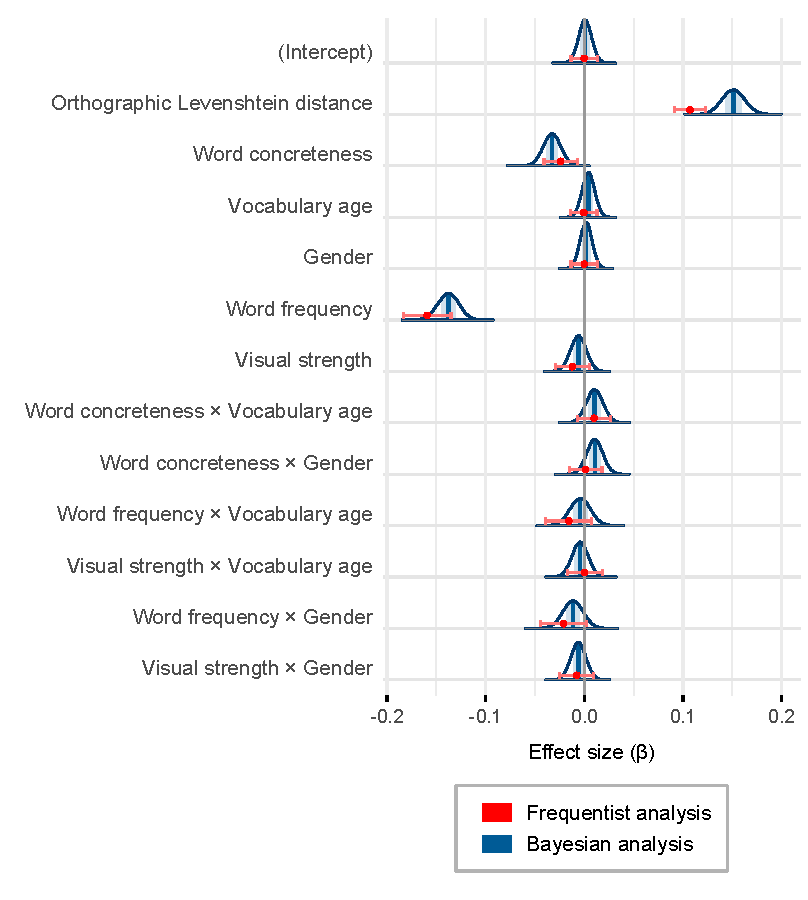
\includegraphics[width=1\linewidth]{C:/Users/Pablo/Documents/semanticpriming-semanticdecision-lexicaldecision/lexicaldecision/frequentist_bayesian_plots/plots/lexicaldecision_frequentist_bayesian_plot_weaklyinformativepriors_exgaussian} 

}

\caption{Estimates for the lexical decision study. The frequentist means (represented by red points) are flanked by 95\% confidence intervals. The Bayesian means (represented by blue vertical lines) are flanked by 95\% credible intervals in light blue.}\label{fig:lexicaldecision-frequentist-bayesian-plot-weaklyinformativepriors-exgaussian}
\end{figure}

Figure \ref{fig:lexicaldecision-interactions-with-vocabulary-age} presents the interactions of vocabulary age with word frequency and with visual strength, both non-significant. Figure \ref{fig:lexicaldecision-interactions-with-gender} shows the interactions with gender, both non-significant too.\footnote{Further interaction plots available in \protect\hyperlink{appendix-D-interaction-plots}{\underline{Appendix D}}.}



\begin{figure}

{\centering 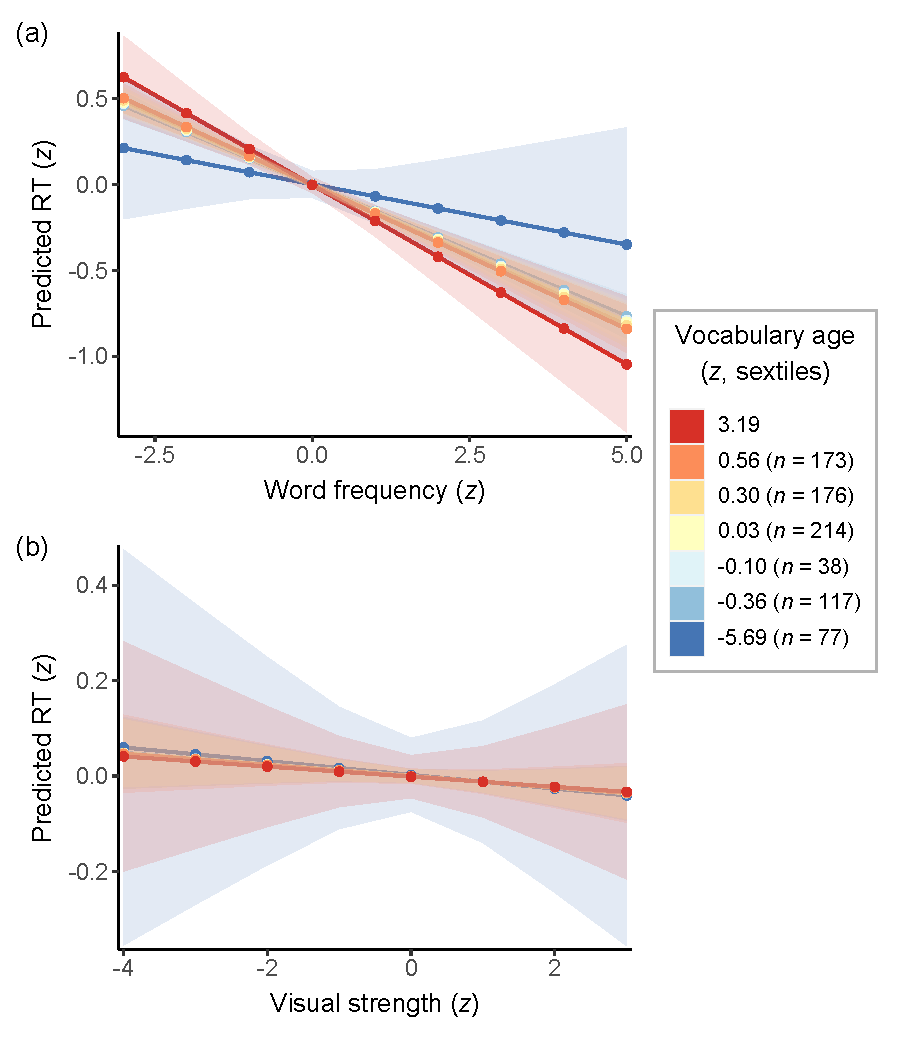
\includegraphics[width=0.8\linewidth]{C:/Users/Pablo/Documents/semanticpriming-semanticdecision-lexicaldecision/lexicaldecision/frequentist_analysis/plots/lexicaldecision-interactions-with-vocabulary-age} 

}

\caption{Interactions of vocabulary age with word frequency (panel a) and with visual strength (panel b). Vocabulary age is constrained to sextiles (6 sections) in this plot, whereas in the statistical analysis it contained more values within the current range. Sextiles were used because there was not enough data for deciles nor for octiles. \(n\) = number of participants contained between sextiles.}\label{fig:lexicaldecision-interactions-with-vocabulary-age}
\end{figure}

\begin{figure}

{\centering 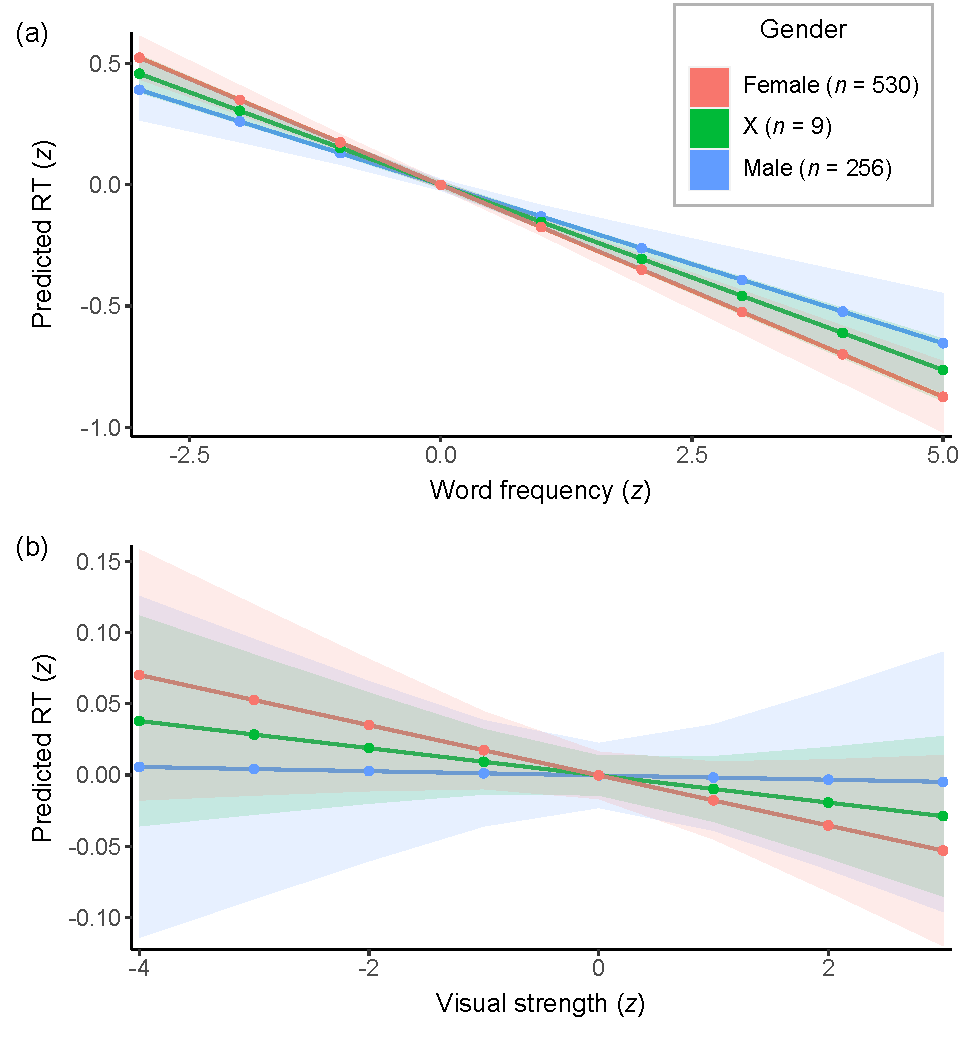
\includegraphics[width=0.8\linewidth]{C:/Users/Pablo/Documents/semanticpriming-semanticdecision-lexicaldecision/lexicaldecision/frequentist_analysis/plots/lexicaldecision-interactions-with-gender} 

}

\caption{Interactions of gender with word frequency (panel a) and with visual strength (panel b) in the lexical decision study. Gender was analysed using $z$-scores, but for clarity, the basic labels are used in the legend.}\label{fig:lexicaldecision-interactions-with-gender}
\end{figure}

\hypertarget{statistical-power-analysis-6}{%
\subsubsection{Statistical power analysis}\label{statistical-power-analysis-6}}

Figures \ref{fig:lexicaldecision-powercurve-plots-1-2-3} and \ref{fig:lexicaldecision-powercurve-plots-4-5-6-7} show the estimated power for some main effects and interactions of interest as a function of the number of participants. To plan the sample size for future studies, these results must be considered under the assumptions that the future study would apply a statistical method similar to ours---namely, a mixed-effects model with random intercepts and slopes---, and that the analysis would encompass at least as many words as the current study, namely, 12,636 (distributed in various blocks across participants, not all being presented to every participant). Furthermore, it is necessary to consider each figure in detail. Here, we provide a summary. First, detecting the main effect of word frequency would require 100 participants. Second, detecting the interactions of word frequency and visual strength with vocabulary size would require 1,500 participants. Third, detecting the other effects would require more than 2,000 participants.

\begin{figure}

{\centering 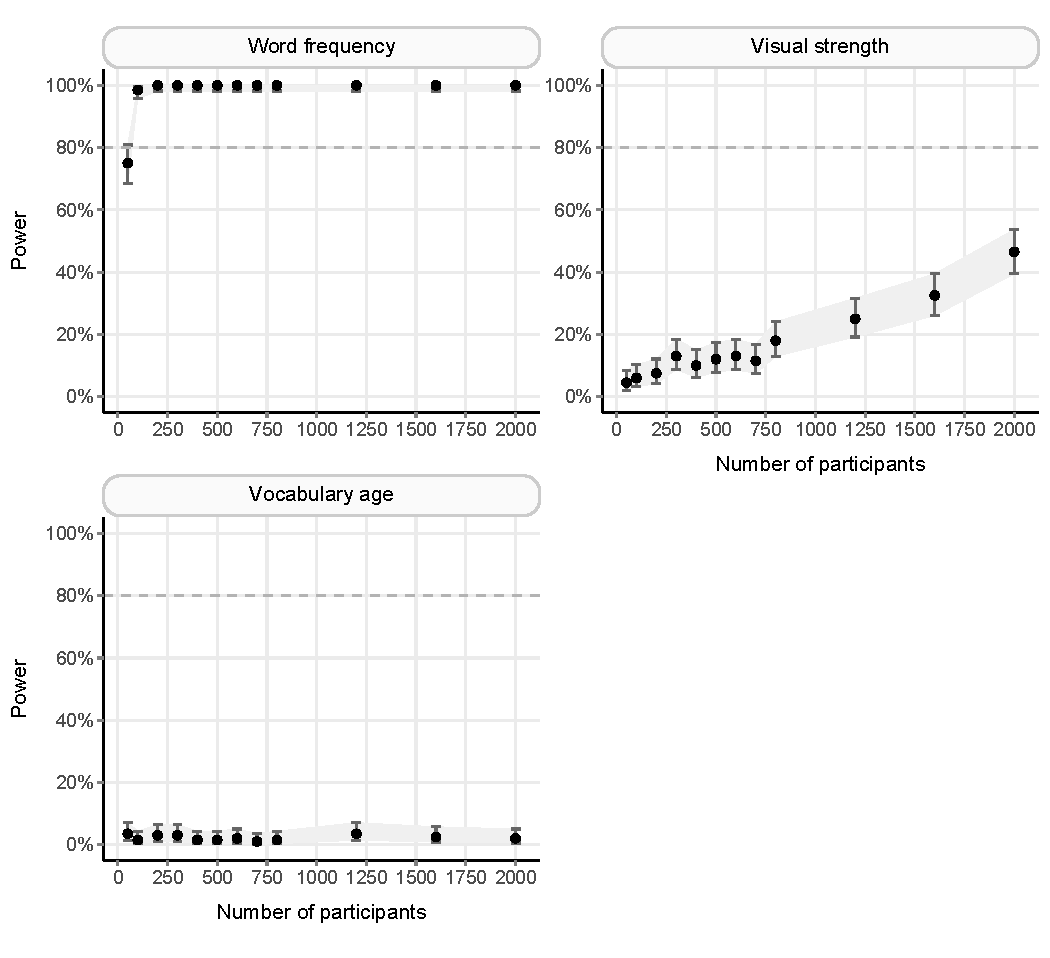
\includegraphics[width=1\linewidth]{C:/Users/Pablo/Documents/semanticpriming-semanticdecision-lexicaldecision/lexicaldecision/power_analysis/plots/lexicaldecision_powercurve_plots_1_2_3} 

}

\caption{Power curves for some main effects in the lexical decision study.}\label{fig:lexicaldecision-powercurve-plots-1-2-3}
\end{figure}

\begin{figure}

{\centering 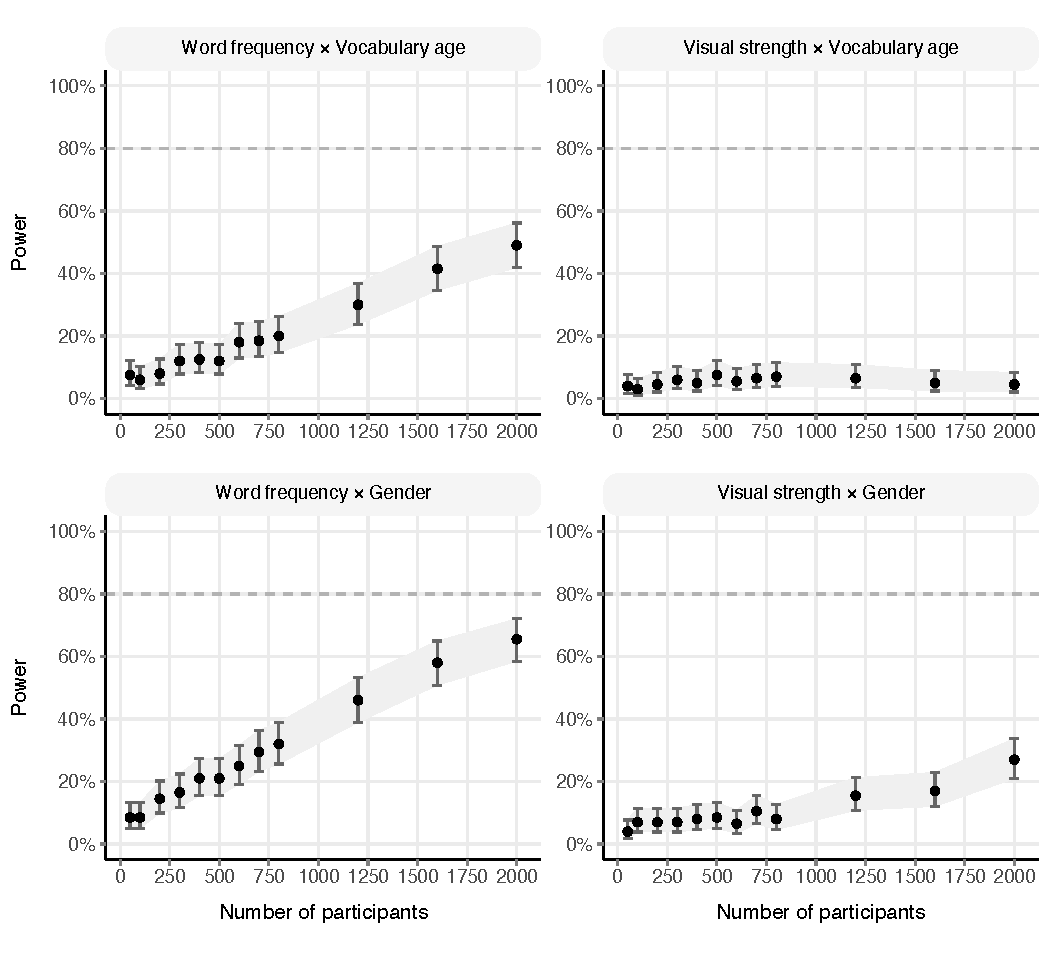
\includegraphics[width=1\linewidth]{C:/Users/Pablo/Documents/semanticpriming-semanticdecision-lexicaldecision/lexicaldecision/power_analysis/plots/lexicaldecision_powercurve_plots_4_5_6_7} 

}

\caption{Power curves for some interactions in the lexical decision study.}\label{fig:lexicaldecision-powercurve-plots-4-5-6-7}
\end{figure}

\hypertarget{discussion-of-study-3}{%
\subsection{Discussion of Study 3}\label{discussion-of-study-3}}

In the present study, we have delved into a task that is likely to elicit a shallower level of semantic processing than the tasks from the previous studies. Furthermore, the data set used in this study was considerably smaller (19,828 RTs, compared to 345,666 RTs in Study 1 and 246,432 in Study 2). The relatively small size of the data set of Study 3 was due to the small number of words per participant (\(M\) = 25) and participants per word (\(M\) = 2 participants per word). In this regard, the English Lexicon Project (Balota et al., 2007) prioritised the total number of words included in their archive.

While the covariates presented large effects, none of the effects of interest turned out to be significant or noteworthy. Furthermore, he comparison with the two previous tasks is hindered by the major difference in the size of the data sets. Therefore, while it is reasonable to find smaller semantic effects in the lexical decision task than in the other two, we cannot reliably attribute this difference to the nature of the task.

As a minor suggestion, future studies could operationalise language using a measure of orthographic neighbourhood size (e.g., orthographic Levenshtein distance), instead of using word frequency as in the present study. While we used word frequency guided by a data-driven selection (see Appendix A), neighbourhood size is a measure created for the purpose of indexing word co-occurrence where only one word is directly available to the researcher (Suárez et al., 2011; Yap \& Balota, 2009).

\hypertarget{statistical-power-analysis-7}{%
\subsubsection{Statistical power analysis}\label{statistical-power-analysis-7}}

We analysed the statistical power associated with several effects of interest, across various sample sizes. The results of this power analysis can help determine the number of participants required to reliably examine each of these effects in a future study. Importantly, the results assume two conditions. First, the future study would apply a statistical method similar to ours---namely, a mixed-effects model with random intercepts and slopes. Second, the analysis of the future study would encompass at least 12,636 stimulus words (distributed in various blocks across participants, not all being presented to every participant).

The results revealed that detecting the main effect of word frequency would require 100 participants. In contrast, detecting the other effects would require more than 2,000 participants.

\hypertarget{general-discussion-of-study-2}{%
\section{General discussion of Study 2}\label{general-discussion-of-study-2}}

In the present study, we have revisited three existing data sets in conceptual processing to investigate the interplay between language-based and vision-based information. Specifically, we have investigated how this interplay is modulated by individual differences in vocabulary size, by the linguistic and visual information contained in words, and by contextual demands such as semantic depth and presentation speed. Although both language and vision played significant roles in some contexts (detailed below), the main effects and the interactions of language-based information were larger than those of vision-based information, consistent with previous research (Banks et al., 2021; Kiela \& Bottou, 2014; Lam et al., 2015; Louwerse et al., 2015; Pecher et al., 1998; Petilli et al., 2021).

In our current approach, the sensorimotor domain was represented by a single variable in each study, just as the language domain was represented by a single variable. In the sensorimotor domain, we focussed on the vision to its hegemonic role in the human brain (Reilly et al., 2020) as well as in several languages (Bernabeu, 2018; Chen et al., 2019; Lynott et al., 2020; Miceli et al., 2021; Morucci et al., 2019; Roque et al., 2015; Speed \& Brybaert, 2021; Speed \& Majid, 2020; Vergallito et al., 2020; Winter et al., 2018; Zhong et al., 2022). Notably, vision was also the domain chosen in a recent study that strongly influenced the present study (Petilli et al., 2021), as well as in previous studies (Bottini et al., 2021; De Deyne et al., 2021; Pearson \& Kosslyn, 2015; Yee et al., 2012). In contrast to this parsimonious approach, more comprehensive alternatives could be used in future research to consider more sensorimotor domains. The first of these approaches is the preselection approach, which incorporates a step prior to the main analysis. In this prior step, a selection is performed among a large variety of word-level information, including visual, auditory and motor information, etc. (Bernabeu et al., 2021). Selecting a single variable provides a convenient way to compare the role of sensorimotor information to that of linguistic information, if the latter is also represented by a single variable. The second approach is using a variable that aggregates sensorimotor information (Wingfield \& Connell, 2022b). Last, the third approach would be using more than one variable to represent sensorimotor information in the main analysis. This would complicate the analysis of interactions with other variables, as the overall number of terms in the model could quickly exceed the maximum normally encountered in mixed-effects models---that is, around 15. If random slopes are included for all those effects of interest (see Brauer \& Curtin, 2018; Singmann \& Kellen, 2019), the model would most likely present convergence warnings. In the face of this challenge, authors could either probe into those warnings (see \protect\hyperlink{appendix-B-frequentist-analysis-diagnostics}{\underline{Appendix B}}), or could opt for different method, such as linear regression or machine learning. Ultimately, in any selection of variables, there is a trade-off between parsimony and comprehensiveness, and negotiating this trade-off often involves a certain degree of arbitrariness. A time-consuming, stepwise selection can help reduce this arbitrariness (for an example, see \protect\hyperlink{appendix-A-lexical-covariates}{\underline{Appendix A}}).

Insofar as both `language' and `vision' were present in the models, it is (arguably) valid to make conclusions based on them (see Louwerse, 2011; Louwerse \& Connell, 2011; Santos et al., 2011; Simmons et al., 2008). In contrast, when only one of these variables is analysed, it may contain information from the other variable. If the superiority of language is genuine---rather than due to a bogus reflection of sensorimotor information---, the present results suggest that language is the main source of information in conceptual processing, whereas sensorimotor information provides extra help, especially for higher-vocabulary individuals (see Study 2, Semantic decision) and in deeper semantic tasks (refer to task-relevance advantage above). As the ultimate conclusion, should sensorimotor simulation be considered smaller but nonetheless important---especially for some individuals and in some contexts---, or should it be considered a negligible by-product of conceptual processing (Mahon \& Caramazza, 2008)? Although the jury is still out, the present results provide support for the tenet that sensorimotor simulation is smaller yet important, especially for some individuals and in some contexts, whereas language is important across the board.

Furthermore, it is necessary to acknowledge a longstanding caveat in the present topic, which also affects the present study. That is, it is extremely difficult to ascertain whether our variables encode what we intend for them to encode. Specifically, it is possible that the variables for language-based information encode some sensorimotor information, and vice versa. To address this caveat, future research could combine the use of continuous word-level variables---as used in the present study---with the use of brain-level measurements (see Borghesani et al., 2016). Specifically, such an investigation should examine whether language-based information is primarily circumscribed to the brain regions in charge of semantic retrieval---such as the posterior left inferior frontal gyrus, the right posterior inferior frontal gyrus, the left anterior superior temporal gyrus and sulcus, and the left middle and posterior middle temporal gyrus (Hagoort, 2017; Skeide \& Friederici, 2016). Conversely, this investigation should also examine whether vision-based information is primarily circumscribed to the brain regions in charge of visual semantic information---such as Brodmann area 17, in the occipital lobe, corresponding to primary visual cortex (Borghesani et al., 2016). Due to the importance of the time course, a method that provides both spatial and temporal resolution, such as magnetoencephalography, would be ideally suited for this research. If both sources of information are largely circumscribed to their regions of interest in the brain, we could conclude that the variables are valid. In contrast, if there are \emph{drifts} in the processing---whereby language-based information is consistently associated with activation in primary visual cortex, or whereby vision-based information is associated with activation in the language regions of interest---, we would need to question the validity of the variables.

As an alternative to the above design, a thriftier method would be available by using two clusters of covariates. One of these clusters would be primarily associated with language-based information, whereas the other cluster would be primarily associated with vision-based information.\footnote{Thank you to Prof.~Max Louwerse for suggesting this idea.} This research should examine whether the variables in each cluster all behave similarly, or whether---instead---there are any drifts between the language and vision. As in the above design, the absence of drifts would validate the operationalisation of the two sides in the dichotomy, whereas the presence of drifts would question the validity.

The present analysis controlled important sources of variance in the fixed effects and in the random effects. First, in the fixed effects, covariates such as word concreteness and individual differences in general cognition were included in the models. It was important to include these covariates as they were substantially correlated with some of our variables of interest, and research has suggested that these covariates may represent fundamentally different processes from those of our variables of interest. For instance, word concreteness and visual strength were highly correlated. However, whereas visual strength indexes a perceptual component of semantic information, word concreteness might be circumscribed to the lexical level, which does not require the processing of meaning (Bottini et al., 2021; cf. Connell \& Lynott, 2012; Pexman \& Yap, 2018). Similarly, it was important to control for individual differences in general cognition measures as covariates of vocabulary size (Ratcliff et al., 2010; also see James et al., 2018; Pexman \& Yap, 2018). We contend that controlling (or, in other words, statistically adjusting) for important covariates is a valuable asset of our present research. Furthermore, we think that the number of covariates we selected was enough but not excessive. We did not find any signs of overfitting in the models, as the variables that have been consistently influential in the literature were also influential in our current models. To further delve into the role of covariates in conceptual processing, we think that it would be valuable to investigate how the presence and the absence of several covariates in a model can affect the effect sizes and the significance results.\footnote{Thank you to Prof.~Max Louwerse for this idea.} Indeed, the differences between the results of Study 1 (semantic priming) and the results of Petilli et al. (2021) suggested that the influence of covariates can be very important. However, because these analyses differed in other aspects of the models, a study focussed on covariates would be insightful (see Botvinik-Nezer et al., 2020; Perret \& Bonin, 2019; Wagenmakers et al., 2022).

Second, in the random effects, the models contained a maximal structure that accounted for far more variance than the fixed effects, thus providing for a conservative analysis. Indeed, the maximal random-effects structure served to impede a violation of the independence of observations (Barr et al., 2013; Brauer \& Curtin, 2018; Singmann \& Kellen, 2019). Specifically, random intercepts and slopes ensured that sources of dependence such as participants and stimuli were kept outside of the fixed effects, which are the relevant effects for the conclusions of this (and most other) research in conceptual processing.

The RTs of higher-vocabulary participants were influenced by a smaller number of variables than those of lower-vocabulary participants. This converges with previous findings suggesting that higher and lower-vocabulary participants are affected by different variables. In this regard, some research has suggested that the variables affecting higher-vocabulary participants most are especially relevant to the task (Lim et al., 2020; Pexman \& Yap, 2018; Yap et al., 2012, 2017). Our results were consistent with the `task-relevance advantage' associated with greater vocabulary knowledge. Specifically, in lexical decision, higher-vocabulary participants were more sensitive than lower-vocabulary participants to language-based information. In contrast, in semantic decision, higher-vocabulary participants were more sensitive to word concreteness. In summary, the present findings suggest that greater linguistic experience may be associated with greater task adaptabiity during cognitive performance, with better comprehenders able to selectively attend to task-relevant features compared to poorer comprehenders (Lim et al., 2020; Pexman \& Yap, 2018).

In addition, the semantic priming paradigm analysed in Study 1 revealed that both language and vision were more important with the short SOA (200 ms) than with the long SOA (1,200 ms). This finding replicates some of the previous literature (Petilli et al., 2021) while highlighting the importance of the time course and the level of semantic processing. That is, although the finding seems to be at odds with the theory that perceptual simulation peaks after language-based associations (Barsalou et al., 2008; Louwerse \& Connell, 2011), the long SOA may have been too long for perceptual simulation to be maintained in the lexical decision task that was performed by participants, which is semantically shallow (Petilli et al., 2021).

\hypertarget{operationalisation-of-variables-and-other-analytical-choices}{%
\subsection{Operationalisation of variables and other analytical choices}\label{operationalisation-of-variables-and-other-analytical-choices}}

We compared two measures of vision-based priming. The first measure---\texttt{visual-strength\ difference}---was operationalised as the difference in visual strength (Lynott et al., 2020) between the prime word and the target word in each trial. The second measure---\texttt{vision-based\ similarity}---, created by Petilli et al. (2021), was based on vector representations trained on images. The results revealed that both measures---including their interactions with other variables---produced similar effect sizes. This underscores the consistency that exists between human ratings and computational approximations to meaning (e.g., Charbonnier \& Wartena, 2019, 2020; Günther et al., 2016b; Louwerse et al., 2015; Mandera et al., 2017; Petilli et al., 2021; Solovyev, 2021; Wingfield \& Connell, 2022a). However, the effect of the human-based variable was slightly larger, which is consistent with previous comparisons of human-based and computational measures (De Deyne et al., 2016, 2019; Gagné et al., 2016; Schmidtke et al., 2018; cf. Michaelov et al., 2022; Snefjella \& Blank, 2020).

In contrast to the results of Petilli et al. (2021), vision-based similarity did not significantly interact with SOA. Furthermore, in contrast to the main analysis, this sub-analysis did not present a significant interaction between language-based similarity and SOA. These two differences demonstrate how the results of our analyses can be critically influenced by analytical choices such as the operationalisation of variables and the degree of complexity of statistical models. In this regard, we must draw attention to an often-overlooked difference between the variables used to operationalise the language system---usually, text-based measures based on large corpora---and the variables used to operationalise the embodiment system---usually, human-based measures based on ratings. Critically, the literature contains many comparisons of text-based variables (De Deyne et al., 2013, 2016; Günther et al., 2016a, 2016b; M. N. Jones et al., 2006; Lund \& Burgess, 1996; Mandera et al., 2017; Mikolov et al., 2013; Wingfield \& Connell, 2022a), whereas the work on embodiment variables is more sparse and tends to compare different \emph{modalities}---e.g., valence, visual strength, auditory strength, etc. (Lynott et al., 2020; Lynott \& Connell, 2009; Newcombe et al., 2012; for an exception, see Vergallito et al., 2020). This accident of history might in part account for the superiority of linguistic information over embodied information (see Banks et al., 2021; Kiela \& Bottou, 2014; Lam et al., 2015; Louwerse et al., 2015; Pecher et al., 1998; Petilli et al., 2021). Therefore, it may be important to consider whether \emph{engineering work} should be devoted to the betterment of embodiment variables. On a more general conclusion, the present results suggest that research findings are fundamentally dependent on research methods.

\hypertarget{statistical-power}{%
\subsection{Statistical power}\label{statistical-power}}

Power analyses were performed to estimate the sample sizes required to reliably investigate a range of effects. The results suggested that 300 participants were sufficient to examine the effect of language-based information contained in words, whereas more than 1,000 participants were necessary for the effect of vision-based information and for the interactions of both former variables with vocabulary size, gender and presentation speed. Regarding interactions specifically, The large sample sizes required to investigate some of the effects relevant to embodied cognition and individual differences are not easily attainable with the usual organisation of funding in Psychology and Neuroscience.

\clearpage

\hypertarget{references}{%
\section{References}\label{references}}

\hypertarget{refs}{}
\begin{CSLReferences}{1}{0}
\leavevmode\vadjust pre{\hypertarget{ref-al-azaryCanYouTouch2022}{}}%
Al-Azary, H., Yu, T., \& McRae, K. (2022). Can you touch the {N400}? {The} interactive effects of body-object interaction and task demands on {N400} amplitudes and decision latencies. \emph{Brain and Language}, \emph{231}, 105147. \url{https://doi.org/10.1016/j.bandl.2022.105147}

\leavevmode\vadjust pre{\hypertarget{ref-albersWhenPowerAnalyses2018}{}}%
Albers, C., \& Lakens, D. (2018). When power analyses based on pilot data are biased: {Inaccurate} effect size estimators and follow-up bias. \emph{Journal of Experimental Social Psychology}, \emph{74}, 187--195. \url{https://doi.org/10.1016/j.jesp.2017.09.004}

\leavevmode\vadjust pre{\hypertarget{ref-amselTrackingRealtimeNeural2011}{}}%
Amsel, B. D. (2011). Tracking real-time neural activation of conceptual knowledge using single-trial event-related potentials. \emph{Neuropsychologia}, \emph{49}(5), 970--983. \url{https://doi.org/10.1016/j.neuropsychologia.2011.01.003}

\leavevmode\vadjust pre{\hypertarget{ref-amselEmpiricallyGroundingGrounded2014}{}}%
Amsel, B. D., Urbach, T. P., \& Kutas, M. (2014). Empirically grounding grounded cognition: {The} case of color. \emph{NeuroImage}, \emph{99}, 149--157. \url{https://doi.org/10.1016/j.neuroimage.2014.05.025}

\leavevmode\vadjust pre{\hypertarget{ref-andersonResponseCommentEstimating2016}{}}%
Anderson, C. J., Bahník, Š., Barnett-Cowan, M., Bosco, F. A., Chandler, J., Chartier, C. R., Cheung, F., Christopherson, C. D., Cordes, A., Cremata, E. J., Della Penna, N., Estel, V., Fedor, A., Fitneva, S. A., Frank, M. C., Grange, J. A., Hartshorne, J. K., Hasselman, F., Henninger, F., \ldots{} Zuni, K. (2016). Response to {Comment} on {``{Estimating} the reproducibility of psychological science.''} \emph{Science}, \emph{351}(6277), 1037--1037. \url{https://doi.org/10.1126/science.aad9163}

\leavevmode\vadjust pre{\hypertarget{ref-aujlaLanguageExperiencePredicts2021}{}}%
Aujla, H. (2021). Language experience predicts semantic priming of lexical decision. \emph{Canadian Journal of Experimental Psychology/Revue Canadienne de Psychologie Expérimentale}, \emph{75}(3), 235. \url{https://doi.org/10.1037/cep0000255}

\leavevmode\vadjust pre{\hypertarget{ref-baayenMixedeffectsModelingCrossed2008}{}}%
Baayen, R. H., Davidson, D. J., \& Bates, D. M. (2008). Mixed-effects modeling with crossed random effects for subjects and items. \emph{Journal of Memory and Language}, \emph{59}(4), 390--412. \url{https://doi.org/10.1016/j.jml.2007.12.005}

\leavevmode\vadjust pre{\hypertarget{ref-balotaDepthAutomaticSpreading1986}{}}%
Balota, D. A., \& Lorch, R. F. (1986). Depth of automatic spreading activation: {Mediated} priming effects in pronunciation but not in lexical decision. \emph{Journal of Experimental Psychology: Learning, Memory, and Cognition}, \emph{12}(3), 336--345. \url{https://doi.org/10.1037/0278-7393.12.3.336}

\leavevmode\vadjust pre{\hypertarget{ref-balotaMeanResponseLatency2008}{}}%
Balota, D. A., Yap, M. J., Cortese, M. J., \& Watson, J. M. (2008). Beyond mean response latency: {Response} time distributional analyses of semantic priming. \emph{Journal of Memory and Language}, \emph{59}(4), 495--523. \url{https://doi.org/10.1016/j.jml.2007.10.004}

\leavevmode\vadjust pre{\hypertarget{ref-balota2007a}{}}%
Balota, D. A., Yap, M. J., Hutchison, K. A., Cortese, M. J., Kessler, B., Loftis, B., Neely, J. H., Nelson, D. L., Simpson, G. B., \& Treiman, R. (2007). The {English Lexicon Project}. \emph{Behavior Research Methods}, \emph{39}, 445--459. \url{https://doi.org/10.3758/BF03193014}

\leavevmode\vadjust pre{\hypertarget{ref-banksLinguisticDistributionalKnowledge2021}{}}%
Banks, B., Wingfield, C., \& Connell, L. (2021). Linguistic distributional knowledge and sensorimotor grounding both contribute to semantic category production. \emph{Cognitive Science}, \emph{45}(10), e13055. \url{https://doi.org/10.1111/cogs.13055}

\leavevmode\vadjust pre{\hypertarget{ref-barca2020a}{}}%
Barca, L., Mazzuca, C., \& Borghi, A. (2020). Overusing the pacifier during infancy sets a footprint on abstract words processing. \emph{Journal of Child Language}, \emph{47}(5), 1084--1099. \url{https://doi.org/10.1017/S0305000920000070}

\leavevmode\vadjust pre{\hypertarget{ref-barrRandomEffectsStructure2013}{}}%
Barr, D. J., Levy, R., Scheepers, C., \& Tily, H. J. (2013). Random effects structure for confirmatory hypothesis testing: {Keep} it maximal. \emph{Journal of Memory and Language}, \emph{68}(3), 255--278. \url{https://doi.org/10.1016/j.jml.2012.11.001}

\leavevmode\vadjust pre{\hypertarget{ref-barsalouEstablishingGeneralizableMechanisms2019}{}}%
Barsalou, L. W. (2019). Establishing generalizable mechanisms. \emph{Psychological Inquiry}, \emph{30}(4), 220--230. \url{https://doi.org/10.1080/1047840X.2019.1693857}

\leavevmode\vadjust pre{\hypertarget{ref-barsalouLanguageSimulationConceptual2008}{}}%
Barsalou, L. W., Santos, A., Simmons, W. K., \& Wilson, C. D. (2008). Language and simulation in conceptual processing. In \emph{Symbols and {Embodiment}}. {Oxford University Press}. \url{https://doi.org/10.1093/acprof:oso/9780199217274.003.0013}

\leavevmode\vadjust pre{\hypertarget{ref-bartonWordlengthEffectReading2014}{}}%
Barton, J. J. S., Hanif, H. M., Eklinder Björnström, L., \& Hills, C. (2014). The word-length effect in reading: {A} review. \emph{Cognitive Neuropsychology}, \emph{31}(5-6), 378--412. \url{https://doi.org/10.1080/02643294.2014.895314}

\leavevmode\vadjust pre{\hypertarget{ref-batesFittingLinearMixedeffects2015}{}}%
Bates, D., Mächler, M., Bolker, B., \& Walker, S. (2015). Fitting linear mixed-effects models using {lme4}. \emph{Journal of Statistical Software}, \emph{67}, 1--48. \url{https://doi.org/10.18637/jss.v067.i01}

\leavevmode\vadjust pre{\hypertarget{ref-batesPackageLme42021}{}}%
Bates, D., Maechler, M., Bolker, B., Walker, S., Christensen, R. H. B., Singmann, H., Dai, B., Scheipl, F., Grothendieck, G., Green, P., Fox, J., Brauer, A., \& Krivitsky, P. N. (2021). \emph{Package '{lme4}'}. {CRAN}. \url{https://cran.r-project.org/web/packages/lme4/lme4.pdf}

\leavevmode\vadjust pre{\hypertarget{ref-beckerLongtermSemanticPriming1997}{}}%
Becker, S., Moscovitch, M., Behrmann, M., \& Joordens, S. (1997). Long-term semantic priming: {A} computational account and empirical evidence. \emph{Journal of Experimental Psychology: Learning, Memory, and Cognition}, \emph{23}(5), 1059--1082. \url{https://doi.org/10.1037/0278-7393.23.5.1059}

\leavevmode\vadjust pre{\hypertarget{ref-beilockSportsExperienceChanges2008}{}}%
Beilock, S. L., Lyons, I. M., Mattarella-Micke, A., Nusbaum, H. C., \& Small, S. L. (2008). Sports experience changes the neural processing of action language. \emph{Proceedings of the National Academy of Sciences}, \emph{105}(36), 13269--13273. \url{https://doi.org/10.1073/pnas.0803424105}

\leavevmode\vadjust pre{\hypertarget{ref-bernabeuDutchModalityExclusivity2018}{}}%
Bernabeu, P. (2018). \emph{Dutch modality exclusivity norms for 336 properties and 411 concepts}. {PsyArXiv}. \url{https://doi.org/10.31234/osf.io/s2c5h}

\leavevmode\vadjust pre{\hypertarget{ref-bernabeu2021a}{}}%
Bernabeu, P., Lynott, D., \& Connell, L. (2021). \emph{Preregistration: {The} interplay between linguistic and embodied systems in conceptual processing}. {OSF}. \url{https://osf.io/ftydw}

\leavevmode\vadjust pre{\hypertarget{ref-bernabeu2017a}{}}%
Bernabeu, P., Willems, R. M., \& Louwerse, M. M. (2017). Modality switch effects emerge early and increase throughout conceptual processing: {Evidence} from {ERPs}. In G. Gunzelmann, A. Howes, T. Tenbrink, \& E. J. Davelaar (Eds.), \emph{Proceedings of the 39th {Annual Conference} of the {Cognitive Science Society}} (pp. 1629--1634). {Cognitive Science Society}. \url{https://mindmodeling.org/cogsci2017/papers/0318}

\leavevmode\vadjust pre{\hypertarget{ref-beyersmannEvidenceEmbeddedWord2020}{}}%
Beyersmann, E., Grainger, J., \& Taft, M. (2020). Evidence for embedded word length effects in complex nonwords. \emph{Language, Cognition and Neuroscience}, \emph{35}(2), 235--245. \url{https://doi.org/10.1080/23273798.2019.1659989}

\leavevmode\vadjust pre{\hypertarget{ref-bonnerReversalConcretenessEffect2009}{}}%
Bonner, M. F., Vesely, L., Price, C., Anderson, C., Richmond, L., Farag, C., Avants, B., \& Grossman, M. (2009). Reversal of the concreteness effect in semantic dementia. \emph{Cognitive Neuropsychology}, \emph{26}(6), 568--579. \url{https://doi.org/10.1080/02643290903512305}

\leavevmode\vadjust pre{\hypertarget{ref-borghesaniWordMeaningVentral2016}{}}%
Borghesani, V., Pedregosa, F., Buiatti, M., Amadon, A., Eger, E., \& Piazza, M. (2016). Word meaning in the ventral visual path: {A} perceptual to conceptual gradient of semantic coding. \emph{NeuroImage}, \emph{143}, 128--140. \url{https://doi.org/10.1016/j.neuroimage.2016.08.068}

\leavevmode\vadjust pre{\hypertarget{ref-borghiWordsSocialTools2019}{}}%
Borghi, A. M., Barca, L., Binkofski, F., Castelfranchi, C., Pezzulo, G., \& Tummolini, L. (2019). Words as social tools: {Language}, sociality and inner grounding in abstract concepts. \emph{Physics of Life Reviews}, \emph{29}, 120--153. \url{https://doi.org/10.1016/j.plrev.2018.12.001}

\leavevmode\vadjust pre{\hypertarget{ref-borghiAbstractConceptsExternal2022}{}}%
Borghi, A. M., Shaki, S., \& Fischer, M. H. (2022). Abstract concepts: External influences, internal constraints, and methodological issues. \emph{Psychological Research}. \url{https://doi.org/10.1007/s00426-022-01698-4}

\leavevmode\vadjust pre{\hypertarget{ref-bottiniNatureSemanticPriming2016}{}}%
Bottini, R., Bucur, M., \& Crepaldi, D. (2016). The nature of semantic priming by subliminal spatial words: {Embodied} or disembodied? \emph{Journal of Experimental Psychology: General}, \emph{145}(9), 1160--1176. \url{https://doi.org/10.1037/xge0000197}

\leavevmode\vadjust pre{\hypertarget{ref-bottiniConcretenessAdvantageLexical2021}{}}%
Bottini, R., Morucci, P., D'Urso, A., Collignon, O., \& Crepaldi, D. (2021). The concreteness advantage in lexical decision does not depend on perceptual simulations. \emph{Journal of Experimental Psychology: General}. \url{https://doi.org/10.1037/xge0001090}

\leavevmode\vadjust pre{\hypertarget{ref-botvinik-nezerVariabilityAnalysisSingle2020}{}}%
Botvinik-Nezer, R., Holzmeister, F., Camerer, C. F., Dreber, A., Huber, J., Johannesson, M., Kirchler, M., Iwanir, R., Mumford, J. A., Adcock, R. A., Avesani, P., Baczkowski, B. M., Bajracharya, A., Bakst, L., Ball, S., Barilari, M., Bault, N., Beaton, D., Beitner, J., \ldots{} Schonberg, T. (2020). Variability in the analysis of a single neuroimaging dataset by many teams. \emph{Nature}, \emph{582}(7810, 7810), 84--88. \url{https://doi.org/10.1038/s41586-020-2314-9}

\leavevmode\vadjust pre{\hypertarget{ref-brauer2018a}{}}%
Brauer, M., \& Curtin, J. J. (2018). Linear mixed-effects models and the analysis of nonindependent data: {A} unified framework to analyze categorical and continuous independent variables that vary within-subjects and/or within-items. \emph{Psychological Methods}, \emph{23}(3), 389--411. \url{https://doi.org/10.1037/met0000159}

\leavevmode\vadjust pre{\hypertarget{ref-brunelliereCooccurrenceFrequencyEvaluated2017}{}}%
Brunellière, A., Perre, L., Tran, T., \& Bonnotte, I. (2017). Co-occurrence frequency evaluated with large language corpora boosts semantic priming effects. \emph{Quarterly Journal of Experimental Psychology}, \emph{70}(9), 1922--1934. \url{https://doi.org/10.1080/17470218.2016.1215479}

\leavevmode\vadjust pre{\hypertarget{ref-brysbaertHowManyParticipants2019}{}}%
Brysbaert, M. (2019). How many participants do we have to include in properly powered experiments? {A} tutorial of power analysis with reference tables. \emph{Journal of Cognition}, \emph{2}(1, 1), 16. \url{https://doi.org/10.5334/joc.72}

\leavevmode\vadjust pre{\hypertarget{ref-brysbaertWordRecognitionII2022}{}}%
Brysbaert, M. (2022). Word recognition {II}. In M. J. Snowling, C. Hulme, \& K. Nation, \emph{The science of reading} (pp. 79--101). {John Wiley \& Sons, Ltd}. \url{https://doi.org/10.1002/9781119705116.ch4}

\leavevmode\vadjust pre{\hypertarget{ref-brysbaertWordFrequencyEffect2018a}{}}%
Brysbaert, M., Mandera, P., \& Keuleers, E. (2018). The word frequency effect in word processing: {An} updated review. \emph{Current Directions in Psychological Science}, \emph{27}(1), 45--50. \url{https://doi.org/10.1177/0963721417727521}

\leavevmode\vadjust pre{\hypertarget{ref-brysbaertPowerAnalysisEffect2018}{}}%
Brysbaert, M., \& Stevens, M. (2018). Power analysis and effect size in mixed effects models: A tutorial. \emph{Journal of Cognition}, \emph{1}(1), 9. \url{https://doi.org/10.5334/joc.10}

\leavevmode\vadjust pre{\hypertarget{ref-brysbaertImpactWordPrevalence2016}{}}%
Brysbaert, M., Stevens, M., Mandera, P., \& Keuleers, E. (2016). The impact of word prevalence on lexical decision times: {Evidence} from the {Dutch Lexicon Project} 2. \emph{Journal of Experimental Psychology: Human Perception and Performance}, \emph{42}(3), 441--458. \url{https://doi.org/10.1037/xhp0000159}

\leavevmode\vadjust pre{\hypertarget{ref-brysbaert2014a}{}}%
Brysbaert, M., Warriner, A. B., \& Kuperman, V. (2014). Concreteness ratings for 40 thousand generally known {English} word lemmas. \emph{Behavior Research Methods}, \emph{46}, 904--911. \url{https://doi.org/10.3758/s13428-013-0403-5}

\leavevmode\vadjust pre{\hypertarget{ref-bullinariaExtractingSemanticRepresentations2007}{}}%
Bullinaria, J. A., \& Levy, J. P. (2007). Extracting semantic representations from word co-occurrence statistics: {A} computational study. \emph{Behavior Research Methods}, \emph{39}(3), 510--526. \url{https://doi.org/10.3758/BF03193020}

\leavevmode\vadjust pre{\hypertarget{ref-burknerAdvancedBayesianMultilevel2018}{}}%
Bürkner, P.-C. (2018). Advanced {Bayesian} multilevel modeling with the {R} package {brms}. \emph{The R Journal}, \emph{10}(1), 395--411. \url{https://journal.r-project.org/archive/2018/RJ-2018-017/index.html}

\leavevmode\vadjust pre{\hypertarget{ref-burknerPackageBrms2022}{}}%
Bürkner, P.-C., Gabry, J., Weber, S., Johnson, A., Modrak, M., Badr, H. S., Weber, F., Ben-Shachar, M. S., \& Rabel, H. (2022). \emph{Package '{brms}'}. {CRAN}. \url{https://cran.r-project.org/web/packages/brms/brms.pdf}

\leavevmode\vadjust pre{\hypertarget{ref-burman2008a}{}}%
Burman, D., Bitan, T., \& Both, J. (2008). Sex differences in neural processing of language among children. \emph{Neuropsychologia}, \emph{46, 5}, 1349--1362. \url{https://doi.org/10.1016/j.neuropsychologia.2007.12.021}

\leavevmode\vadjust pre{\hypertarget{ref-buttonPowerFailureWhy2013}{}}%
Button, K. S., Ioannidis, J. P. A., Mokrysz, C., Nosek, B. A., Flint, J., Robinson, E. S. J., \& Munafò, M. R. (2013). Power failure: {Why} small sample size undermines the reliability of neuroscience. \emph{Nature Reviews Neuroscience}, \emph{14}(5, 5), 365--376. \url{https://doi.org/10.1038/nrn3475}

\leavevmode\vadjust pre{\hypertarget{ref-calvo-merinoActionObservationAcquired2005}{}}%
Calvo-Merino, B., Glaser, D. E., Grèzes, J., Passingham, R. E., \& Haggard, P. (2005). Action observation and acquired motor skills: {An} {FMRI} study with expert dancers. \emph{Cerebral Cortex}, \emph{15}(8), 1243--1249. \url{https://doi.org/10.1093/cercor/bhi007}

\leavevmode\vadjust pre{\hypertarget{ref-cerniMotorExpertiseTyping2016}{}}%
Cerni, T., Velay, J.-L., Alario, F.-X., Vaugoyeau, M., \& Longcamp, M. (2016). Motor expertise for typing impacts lexical decision performance. \emph{Trends in Neuroscience and Education}, \emph{5}(3), 130--138. \url{https://doi.org/10.1016/j.tine.2016.07.007}

\leavevmode\vadjust pre{\hypertarget{ref-charbonnierPredictingWordConcreteness2019}{}}%
Charbonnier, J., \& Wartena, C. (2019). Predicting word concreteness and imagery. \emph{Proceedings of the 13th {International Conference} on {Computational Semantics} - {Long Papers}}, 176--187. \url{https://doi.org/10.18653/v1/W19-0415}

\leavevmode\vadjust pre{\hypertarget{ref-charbonnierPredictingConcretenessGerman2020}{}}%
Charbonnier, J., \& Wartena, C. (2020). Predicting the concreteness of {German} words. \emph{Proceedings of the 5th {Swiss Text Analytics Conference} ({SwissText})}, \emph{2624}. \url{https://doi.org/10.25968/opus-2075}

\leavevmode\vadjust pre{\hypertarget{ref-chenMandarinChineseModality2019}{}}%
Chen, I.-H., Zhao, Q., Long, Y., Lu, Q., \& Huang, C.-R. (2019). Mandarin {Chinese} modality exclusivity norms. \emph{PLOS ONE}, \emph{14}(2), e0211336. \url{https://doi.org/10.1371/journal.pone.0211336}

\leavevmode\vadjust pre{\hypertarget{ref-cohenCostDichotomization1983}{}}%
Cohen, J. (1983). The cost of dichotomization. \emph{Applied Psychological Measurement}, \emph{7}(3), 249--253. \url{https://doi.org/10.1177/014662168300700301}

\leavevmode\vadjust pre{\hypertarget{ref-collinsModalitySwitchingProperty2011}{}}%
Collins, J., Pecher, D., Zeelenberg, R., \& Coulson, S. (2011). Modality switching in a property verification task: {An} {ERP} study of what happens when candles flicker after high heels click. \emph{Frontiers in Psychology}, \emph{2}(10). \url{https://doi.org/10.3389/fpsyg.2011.00010}

\leavevmode\vadjust pre{\hypertarget{ref-connell2019a}{}}%
Connell, L. (2019). What have labels ever done for us? {The} linguistic shortcut in conceptual processing. \emph{Language, Cognition and Neuroscience}, \emph{34}(10), 1308--1318. \url{https://doi.org/10.1080/23273798.2018.1471512}

\leavevmode\vadjust pre{\hypertarget{ref-connellStrengthPerceptualExperience2012}{}}%
Connell, L., \& Lynott, D. (2012). Strength of perceptual experience predicts word processing performance better than concreteness or imageability. \emph{Cognition}, \emph{125}(3), 452--465. \url{https://doi.org/10.1016/j.cognition.2012.07.010}

\leavevmode\vadjust pre{\hypertarget{ref-connell2013a}{}}%
Connell, L., \& Lynott, D. (2013). Flexible and fast: {Linguistic} shortcut affects both shallow and deep conceptual processing. \emph{Psychonomic Bulletin \& Review}, \emph{20, 3}, 542--550. \url{https://doi.org/10.3758/s13423-012-0368-x}

\leavevmode\vadjust pre{\hypertarget{ref-connellSeeHearWhat2014}{}}%
Connell, L., \& Lynott, D. (2014). I see/hear what you mean: {Semantic} activation in visual word recognition depends on perceptual attention. \emph{Journal of Experimental Psychology: General}, \emph{143}(2), 527--533. \url{https://doi.org/10.1037/a0034626}

\leavevmode\vadjust pre{\hypertarget{ref-connellInteroceptionForgottenModality2018}{}}%
Connell, L., Lynott, D., \& Banks, B. (2018). Interoception: The forgotten modality in perceptual grounding of abstract and concrete concepts. \emph{Philosophical Transactions of the Royal Society B: Biological Sciences}, \emph{373}(1752), 20170143. \url{https://doi.org/10.1098/rstb.2017.0143}

\leavevmode\vadjust pre{\hypertarget{ref-corkerHighQualityDirect2014}{}}%
Corker, K. S., Lynott, D., Wortman, J., Connell, L., Donnellan, M. B., Lucas, R. E., \& O'Brien, K. (2014). High quality direct replications matter: {Response} to {Williams} (2014). \emph{Social Psychology}, \emph{45}(4), 324--326.

\leavevmode\vadjust pre{\hypertarget{ref-cummingNewStatisticsWhy2014}{}}%
Cumming, G. (2014). The new statistics: {Why} and how. \emph{Psychological Science}, \emph{25}(1), 7--29. \url{https://doi.org/10.1177/0956797613504966}

\leavevmode\vadjust pre{\hypertarget{ref-daidoneVocabularySizeKey2021}{}}%
Daidone, D., \& Darcy, I. (2021). Vocabulary size is a key factor in predicting second language lexical encoding accuracy. \emph{Frontiers in Psychology}, \emph{12}, 688356. \url{https://doi.org/10.3389/fpsyg.2021.688356}

\leavevmode\vadjust pre{\hypertarget{ref-davies2017a}{}}%
Davies, R. A., Arnell, R., Birchenough, J. M., Grimmond, D., \& Houlson, S. (2017). Reading through the life span: {Individual} differences in psycholinguistic effects. \emph{Journal of Experimental Psychology: Learning, Memory, and Cognition}, \emph{43}(8), 1298. \url{https://doi.org/10.1037/xlm0000366}

\leavevmode\vadjust pre{\hypertarget{ref-davisBuildingSemanticMemory2021}{}}%
Davis, C. P., \& Yee, E. (2021). Building semantic memory from embodied and distributional language experience. \emph{WIREs Cognitive Science}, \emph{12}(5), e1555. \url{https://doi.org/10.1002/wcs.1555}

\leavevmode\vadjust pre{\hypertarget{ref-dedeyneVisualAffectiveMultimodal2021}{}}%
De Deyne, S., Navarro, D. J., Collell, G., \& Perfors, A. (2021). Visual and affective multimodal models of word meaning in language and mind. \emph{Cognitive Science}, \emph{45}(1), e12922. \url{https://doi.org/10.1111/cogs.12922}

\leavevmode\vadjust pre{\hypertarget{ref-de2019a}{}}%
De Deyne, S., Navarro, D. J., Perfors, A., Brysbaert, M., \& Storms, G. (2019). The {``{Small World} of {Words}''} {English} word association norms for over 12,000 cue words. \emph{Behavior Research Methods}, \emph{51}, 987--1006. \url{https://doi.org/10.3758/s13428-018-1115-7}

\leavevmode\vadjust pre{\hypertarget{ref-dedeyneBetterExplanationsLexical2013}{}}%
De Deyne, S., Navarro, D. J., \& Storms, G. (2013). Better explanations of lexical and semantic cognition using networks derived from continued rather than single-word associations. \emph{Behavior Research Methods}, \emph{45}(2), 480--498. \url{https://doi.org/10.3758/s13428-012-0260-7}

\leavevmode\vadjust pre{\hypertarget{ref-de2016a}{}}%
De Deyne, S., Perfors, A., \& Navarro, D. (2016). Predicting human similarity judgments with distributional models: {The} value of word associations. \emph{Proceedings of {COLING} 2016, the 26th International Conference on Computational Linguistics: {Technical} Papers}, 1861--1870.

\leavevmode\vadjust pre{\hypertarget{ref-dewitMaskedSemanticPriming2015}{}}%
de Wit, B., \& Kinoshita, S. (2015). The masked semantic priming effect is task dependent: {Reconsidering} the automatic spreading activation process. \emph{Journal of Experimental Psychology: Learning, Memory, and Cognition}, \emph{41}(4), 1062--1075. \url{https://doi.org/10.1037/xlm0000074}

\leavevmode\vadjust pre{\hypertarget{ref-delucaRedefiningBilingualismSpectrum2019}{}}%
DeLuca, V., Rothman, J., Bialystok, E., \& Pliatsikas, C. (2019). Redefining bilingualism as a spectrum of experiences that differentially affects brain structure and function. \emph{Proceedings of the National Academy of Sciences}, \emph{116}(15), 7565--7574. \url{https://doi.org/10.1073/pnas.1811513116}

\leavevmode\vadjust pre{\hypertarget{ref-diazNeuralSensitivityPhonological2021}{}}%
Diaz, M. T., Karimi, H., Troutman, S. B. W., Gertel, V. H., Cosgrove, A. L., \& Zhang, H. (2021). Neural sensitivity to phonological characteristics is stable across the lifespan. \emph{NeuroImage}, \emph{225}, 117511. \url{https://doi.org/10.1016/j.neuroimage.2020.117511}

\leavevmode\vadjust pre{\hypertarget{ref-dijkstraMultilinkComputationalModel2019}{}}%
Dijkstra, T., Wahl, A., Buytenhuijs, F., Halem, N. V., Al-Jibouri, Z., Korte, M. D., \& Rekké, S. (2019). Multilink: {A} computational model for bilingual word recognition and word translation. \emph{Bilingualism: Language and Cognition}, \emph{22}(4), 657--679. \url{https://doi.org/10.1017/S1366728918000287}

\leavevmode\vadjust pre{\hypertarget{ref-dils2010a}{}}%
Dils, A. T., \& Boroditsky, L. (2010). Visual motion aftereffect from understanding motion language. \emph{Proceedings of the National Academy of Sciences}, \emph{107}(37), 16396--16400. \url{https://doi.org/10.1073/pnas.1009438107}

\leavevmode\vadjust pre{\hypertarget{ref-diveicaQuantifyingSocialSemantics2022}{}}%
Diveica, V., Pexman, P. M., \& Binney, R. J. (2022). Quantifying social semantics: {An} inclusive definition of socialness and ratings for 8388 {English} words. \emph{Behavior Research Methods}. \url{https://doi.org/10.3758/s13428-022-01810-x}

\leavevmode\vadjust pre{\hypertarget{ref-dormannCollinearityReviewMethods2013}{}}%
Dormann, C. F., Elith, J., Bacher, S., Buchmann, C., Carl, G., Carré, G., Marquéz, J. R. G., Gruber, B., Lafourcade, B., Leitão, P. J., Münkemüller, T., McClean, C., Osborne, P. E., Reineking, B., Schröder, B., Skidmore, A. K., Zurell, D., \& Lautenbach, S. (2013). Collinearity: A review of methods to deal with it and a simulation study evaluating their performance. \emph{Ecography}, \emph{36}(1), 27--46. \url{https://doi.org/10.1111/j.1600-0587.2012.07348.x}

\leavevmode\vadjust pre{\hypertarget{ref-dunabeitiaQualitativeDifferencesRepresentation2009}{}}%
Duñabeitia, J. A., Avilés, A., Afonso, O., Scheepers, C., \& Carreiras, M. (2009). Qualitative differences in the representation of abstract versus concrete words: {Evidence} from the visual-world paradigm. \emph{Cognition}, \emph{110}(2), 284--292. \url{https://doi.org/10.1016/j.cognition.2008.11.012}

\leavevmode\vadjust pre{\hypertarget{ref-faust1999a}{}}%
Faust, M. E., Balota, D. A., Spieler, D. H., \& Ferraro, F. R. (1999). Individual differences in information-processing rate and amount: {Implications} for group differences in response latency. \emph{Psychological Bulletin}, \emph{125}, 777--799. \url{https://doi.org/10.1037/0033-2909.125.6.777}

\leavevmode\vadjust pre{\hypertarget{ref-fernandinoDecodingInformationStructure2022}{}}%
Fernandino, L., Tong, J.-Q., Conant, L. L., Humphries, C. J., \& Binder, J. R. (2022). Decoding the information structure underlying the neural representation of concepts. \emph{Proceedings of the National Academy of Sciences}, \emph{119}(6). \url{https://doi.org/10.1073/pnas.2108091119}

\leavevmode\vadjust pre{\hypertarget{ref-fettermanFeelingWarmBeing2018}{}}%
Fetterman, A. K., Wilkowski, B. M., \& Robinson, M. D. (2018). On feeling warm and being warm: {Daily} perceptions of physical warmth fluctuate with interpersonal warmth. \emph{Social Psychological and Personality Science}, \emph{9}(5), 560--567. \url{https://doi.org/10.1177/1948550617712032}

\leavevmode\vadjust pre{\hypertarget{ref-fleurDefinitelySawIt2020}{}}%
Fleur, D. S., Flecken, M., Rommers, J., \& Nieuwland, M. S. (2020). Definitely saw it coming? {The} dual nature of the pre-nominal prediction effect. \emph{Cognition}, \emph{204}, 104335. \url{https://doi.org/10.1016/j.cognition.2020.104335}

\leavevmode\vadjust pre{\hypertarget{ref-floresdarcaisSemanticActivationRecognition1985}{}}%
Flores d'Arcais, G. B., Schreuder, R., \& Glazenborg, G. (1985). Semantic activation during recognition of referential words. \emph{Psychological Research}, \emph{47}(1), 39--49. \url{https://doi.org/10.1007/BF00309217}

\leavevmode\vadjust pre{\hypertarget{ref-foxGeneralizedLinearModels2016}{}}%
Fox, J. (2016). Generalized linear models. In \emph{Applied regression analysis and generalized linear models} (Third Edition, pp. 418--472). {SAGE}.

\leavevmode\vadjust pre{\hypertarget{ref-NIPS2013_7cce53cf}{}}%
Frome, A., Corrado, G. S., Shlens, J., Bengio, S., Dean, J., Ranzato, M., \& Mikolov, T. (2013). {DeViSE}: {A} deep visual-semantic embedding model. In C. J. Burges, L. Bottou, M. Welling, Z. Ghahramani, \& K. Q. Weinberger (Eds.), \emph{Advances in neural information processing systems} (Vol. 26). {Curran Associates, Inc.} \url{https://proceedings.neurips.cc/paper/2013/file/7cce53cf90577442771720a370c3c723-Paper.pdf}

\leavevmode\vadjust pre{\hypertarget{ref-gagneProcessingEnglishCompounds2016}{}}%
Gagné, C. L., Spalding, T. L., \& Nisbet, K. A. (2016). Processing {English} compounds: {Investigating} semantic transparency. \emph{SKASE Journal of Theoretical Linguistics}, \emph{13}(2), 2--22. \url{https://link.gale.com/apps/doc/A469757337/LitRC?u=anon~b6a332f4\&xid=9960afc7}

\leavevmode\vadjust pre{\hypertarget{ref-galleseBrainConceptsRole2005}{}}%
Gallese, V., \& Lakoff, G. (2005). The {Brain}'s concepts: The role of the {Sensory-motor} system in conceptual knowledge. \emph{Cognitive Neuropsychology}, \emph{22}(3-4), 455--479. \url{https://doi.org/10.1080/02643290442000310}

\leavevmode\vadjust pre{\hypertarget{ref-gelmanPowerCalculationsAssessing2014}{}}%
Gelman, A., \& Carlin, J. (2014). Beyond power calculations: Assessing type {S} (sign) and type {M} (magnitude) errors. \emph{Perspectives on Psychological Science}, \emph{9}(6), 641--651. \url{https://doi.org/10.1177/1745691614551642}

\leavevmode\vadjust pre{\hypertarget{ref-gelmanPosteriorPredictiveAssessment1996}{}}%
Gelman, A., Meng, X., \& Stern, H. (1996). Posterior predictive assessment of model fitness via realized discrepancies. \emph{Statistica Sinica}, 733--807.

\leavevmode\vadjust pre{\hypertarget{ref-gilbertCommentEstimatingReproducibility2016}{}}%
Gilbert, D. T., King, G., Pettigrew, S., \& Wilson, T. D. (2016). Comment on {``{Estimating} the reproducibility of psychological science.''} \emph{Science}, \emph{351}(6277), 1037--1037. \url{https://doi.org/10.1126/science.aad7243}

\leavevmode\vadjust pre{\hypertarget{ref-greenSIMRPackagePower2016}{}}%
Green, P., \& MacLeod, C. J. (2016). {SIMR}: {An R} package for power analysis of generalized linear mixed models by simulation. \emph{Methods in Ecology and Evolution}, \emph{7}(4), 493--498. \url{https://doi.org/10.1111/2041-210X.12504}

\leavevmode\vadjust pre{\hypertarget{ref-guntherLatentSemanticAnalysis2016}{}}%
Günther, F., Dudschig, C., \& Kaup, B. (2016a). Latent semantic analysis cosines as a cognitive similarity measure: {Evidence} from priming studies. \emph{Quarterly Journal of Experimental Psychology}, \emph{69}(4), 626--653. \url{https://doi.org/10.1080/17470218.2015.1038280}

\leavevmode\vadjust pre{\hypertarget{ref-R-LSAfun}{}}%
Günther, F., Dudschig, C., \& Kaup, B. (2015). LSAfun: An r package for computations based on latent semantic analysis. \emph{Behavior Research Methods}, \emph{47}(4), 930--944. \url{https://doi.org/10.3758/s13428-014-0529-0}

\leavevmode\vadjust pre{\hypertarget{ref-guenther2016a}{}}%
Günther, F., Dudschig, C., \& Kaup, B. (2016b). Predicting lexical priming effects from distributional semantic similarities: {A} replication with extension. \emph{Frontiers in Psychology}, \emph{7}, 1646. \url{https://doi.org/10.3389/fpsyg.2016.01646}

\leavevmode\vadjust pre{\hypertarget{ref-hagoortCoreLanguagereadyBrain2017}{}}%
Hagoort, P. (2017). The core and beyond in the language-ready brain. \emph{Neuroscience \& Biobehavioral Reviews}, \emph{81}, 194--204. \url{https://doi.org/10.1016/j.neubiorev.2017.01.048}

\leavevmode\vadjust pre{\hypertarget{ref-haldEEGThetaGamma2006}{}}%
Hald, L. A., Bastiaansen, M. C. M., \& Hagoort, P. (2006). {EEG} theta and gamma responses to semantic violations in online sentence processing. \emph{Brain and Language}, \emph{96}(1), 90--105. \url{https://doi.org/10.1016/j.bandl.2005.06.007}

\leavevmode\vadjust pre{\hypertarget{ref-hald2013a}{}}%
Hald, L. A., Hocking, I., Vernon, D., Marshall, J. A., \& Garnham, A. (2013). Exploring modality switching effects in negated sentences: {Further} evidence for grounded representations. \emph{Frontiers in Psychology}, \emph{4}, 93. \url{https://doi.org/10.3389/fpsyg.2013.00093}

\leavevmode\vadjust pre{\hypertarget{ref-hald2011a}{}}%
Hald, L. A., Marshall, J. A., Janssen, D. P., \& Garnham, A. (2011). Switching modalities in a sentence verification task: {ERP} evidence for embodied language processing. \emph{Frontiers in Psychology}, \emph{2}, 45. \url{https://doi.org/10.3389/fpsyg.2011.00045}

\leavevmode\vadjust pre{\hypertarget{ref-harrison2018a}{}}%
Harrison, X. A., Donaldson, L., Correa-Cano, M. E., Evans, J., Fisher, D. N., Goodwin, C., Robinson, B. S., Hodgson, D. J., \& Inger, R. (2018). A brief introduction to mixed effects modelling and multi-model inference in ecology. \emph{PeerJ}, \emph{6}, 4794. \url{https://doi.org/10.7717/peerj.4794}

\leavevmode\vadjust pre{\hypertarget{ref-haukOnlyTimeWill2016}{}}%
Hauk, O. (2016). Only time will tell -- why temporal information is essential for our neuroscientific understanding of semantics. \emph{Psychonomic Bulletin \& Review}, \emph{23}(4), 1072--1079. \url{https://doi.org/10.3758/s13423-015-0873-9}

\leavevmode\vadjust pre{\hypertarget{ref-hedge2018a}{}}%
Hedge, C., Powell, G., \& Sumner, P. (2018). The reliability paradox: {Why} robust cognitive tasks do not produce reliable individual differences. \emph{Behavior Research Methods}, \emph{50}(3), 1166--1186. \url{https://doi.org/10.3758/s13428-017-0935-1}

\leavevmode\vadjust pre{\hypertarget{ref-heymanReliabilityItemlevelSemantic2018}{}}%
Heyman, T., Bruninx, A., Hutchison, K. A., \& Storms, G. (2018). The (un)reliability of item-level semantic priming effects. \emph{Behavior Research Methods}, \emph{50}(6), 2173--2183. \url{https://doi.org/10.3758/s13428-018-1040-9}

\leavevmode\vadjust pre{\hypertarget{ref-hoedemakerItTakesTime2014}{}}%
Hoedemaker, R. S., \& Gordon, P. C. (2014). It takes time to prime: {Semantic} priming in the ocular lexical decision task. \emph{Journal of Experimental Psychology: Human Perception and Performance}, \emph{40}(6), 2179--2197. \url{https://doi.org/10.1037/a0037677}

\leavevmode\vadjust pre{\hypertarget{ref-hoenigAbusePower2001}{}}%
Hoenig, J. M., \& Heisey, D. M. (2001). The {Abuse} of {Power}. \emph{The American Statistician}, \emph{55}(1), 19--24. \url{https://doi.org/10.1198/000313001300339897}

\leavevmode\vadjust pre{\hypertarget{ref-hoffmanReverseConcretenessEffects2011}{}}%
Hoffman, P., \& Lambon Ralph, M. A. (2011). Reverse concreteness effects are not a typical feature of semantic dementia: {Evidence} for the hub-and-spoke model of conceptual representation. \emph{Cerebral Cortex}, \emph{21}(9), 2103--2112. \url{https://doi.org/10.1093/cercor/bhq288}

\leavevmode\vadjust pre{\hypertarget{ref-holt2006a}{}}%
Holt, L. E., \& Beilock, S. L. (2006). Expertise and its embodiment: {Examining} the impact of sensorimotor skill expertise on the representation of action-related text. \emph{Psychonomic Bulletin \& Review}, \emph{13}(4), 694--701. \url{https://doi.org/10.3758/BF03193983}

\leavevmode\vadjust pre{\hypertarget{ref-hultenNeuralRepresentationAbstract2021}{}}%
Hultén, A., Vliet, M. van, Kivisaari, S., Lammi, L., Lindh-Knuutila, T., Faisal, A., \& Salmelin, R. (2021). The neural representation of abstract words may arise through grounding word meaning in language itself. \emph{Human Brain Mapping}, \emph{42}(15), 4973--4984. \url{https://onlinelibrary.wiley.com/doi/abs/10.1002/hbm.25593}

\leavevmode\vadjust pre{\hypertarget{ref-hutchinson2013a}{}}%
Hutchinson, S., \& Louwerse, M. M. (2013). Language statistics and individual differences in processing primary metaphors. \emph{Cognitive Linguistics}, \emph{24}(4), 667--687. \url{https://doi.org/10.1515/cog-2013-0023}

\leavevmode\vadjust pre{\hypertarget{ref-hutchisonSemanticPrimingDue2003}{}}%
Hutchison, K. A. (2003). Is semantic priming due to association strength or feature overlap? {A} microanalytic review. \emph{Psychonomic Bulletin \& Review}, \emph{10}(4), 785--813. \url{https://doi.org/10.3758/BF03196544}

\leavevmode\vadjust pre{\hypertarget{ref-hutchisonPredictingSemanticPriming2008}{}}%
Hutchison, K. A., Balota, D. A., Cortese, M. J., \& Watson, J. M. (2008). Predicting semantic priming at the item level. \emph{Quarterly Journal of Experimental Psychology}, \emph{61}(7), 1036--1066. \url{https://doi.org/10.1080/17470210701438111}

\leavevmode\vadjust pre{\hypertarget{ref-hutchison2013a}{}}%
Hutchison, K. A., Balota, D. A., Neely, J. H., Cortese, M. J., Cohen-Shikora, E. R., Tse, C.-S., Yap, M. J., Bengson, J. J., Niemeyer, D., \& Buchanan, E. (2013). The semantic priming project. \emph{Behavior Research Methods}, \emph{45}, 1099--1114. \url{https://doi.org/10.3758/s13428-012-0304-z}

\leavevmode\vadjust pre{\hypertarget{ref-hutchisonAttentionalControlAsymmetric2014}{}}%
Hutchison, K. A., Heap, S. J., Neely, J. H., \& Thomas, M. A. (2014). Attentional control and asymmetric associative priming. \emph{Journal of Experimental Psychology: Learning, Memory, and Cognition}, \emph{40}(3), 844--856. \url{https://doi.org/10.1037/a0035781}

\leavevmode\vadjust pre{\hypertarget{ref-james2018a}{}}%
James, A. N., Fraundorf, S. H., Lee, E. K., \& Watson, D. G. (2018). Individual differences in syntactic processing: {Is} there evidence for reader-text interactions? \emph{Journal of Memory and Language}, \emph{102}, 155--181. \url{https://doi.org/10.1016/j.jml.2018.05.006}

\leavevmode\vadjust pre{\hypertarget{ref-jaredSkilledAdultReaders2017}{}}%
Jared, D., \& O'Donnell, K. (2017). Skilled adult readers activate the meanings of high-frequency words using phonology: {Evidence} from eye tracking. \emph{Memory \& Cognition}, \emph{45}(2), 334--346. \url{https://doi.org/10.3758/s13421-016-0661-4}

\leavevmode\vadjust pre{\hypertarget{ref-jonesDistrubutionalSemanticsStill2022}{}}%
Jones, C. R., Chang, T. A., Coulson, S., Michaelov, J. A., Trott, S., \& Bergen, B. (2022). Distrubutional semantics still can't account for affordances. \emph{Proceedings of the Annual Meeting of the Cognitive Science Society}, \emph{44}(44). \url{https://escholarship.org/uc/item/44z7r3j3}

\leavevmode\vadjust pre{\hypertarget{ref-jones2006a}{}}%
Jones, M. N., Kintsch, W., \& Mewhort, D. J. (2006). High-dimensional semantic space accounts of priming. \emph{Journal of Memory and Language}, \emph{55}(4), 534--552. \url{https://doi.org/10.1016/j.jml.2006.07.003}

\leavevmode\vadjust pre{\hypertarget{ref-joordensLongShortSemantic1997}{}}%
Joordens, S., \& Becker, S. (1997). The long and short of semantic priming effects in lexical decision. \emph{Journal of Experimental Psychology: Learning, Memory, and Cognition}, \emph{23}(5), 1083--1105. \url{https://doi.org/10.1037/0278-7393.23.5.1083}

\leavevmode\vadjust pre{\hypertarget{ref-jung2019a}{}}%
Jung, M., Mody, M., Fujioka, T., Kimura, Y., Okazawa, H., \& Kosaka, H. (2019). Sex differences in white matter pathways related to language ability. \emph{Frontiers in Human Neuroscience}, \emph{13}, 898. \url{https://doi.org/10.3389/fnins.2019.00898}

\leavevmode\vadjust pre{\hypertarget{ref-khatin-zadehStrongVersionsEmbodied2021}{}}%
Khatin-Zadeh, O., Eskandari, Z., Cervera-Torres, S., Ruiz Fernández, S., Farzi, R., \& Marmolejo-Ramos, F. (2021). The strong versions of embodied cognition: {Three} challenges faced. \emph{Psychology \& Neuroscience}, \emph{14}(1), 16--33. \url{https://doi.org/10.1037/pne0000252}

\leavevmode\vadjust pre{\hypertarget{ref-kieferDifferentialTemporospatialPattern2022}{}}%
Kiefer, M., Pielke, L., \& Trumpp, N. M. (2022). Differential temporo-spatial pattern of electrical brain activity during the processing of abstract concepts related to mental states and verbal associations. \emph{NeuroImage}, \emph{252}, 119036. \url{https://doi.org/10.1016/j.neuroimage.2022.119036}

\leavevmode\vadjust pre{\hypertarget{ref-kiela2014a}{}}%
Kiela, D., \& Bottou, L. (2014). Learning image embeddings using convolutional neural networks for improved multi-modal semantics. \emph{Proceedings of the 2014 Conference on Empirical Methods in Natural Language Processing ({EMNLP}}, 36--45. \url{https://doi.org/10.3115/v1/D14-1005}

\leavevmode\vadjust pre{\hypertarget{ref-kimEffectsLexicalFeatures2018}{}}%
Kim, M., Crossley, S. A., \& Skalicky, S. (2018). Effects of lexical features, textual properties, and individual differences on word processing times during second language reading comprehension. \emph{Reading and Writing}, \emph{31}(5), 1155--1180. \url{https://doi.org/10.1007/s11145-018-9833-x}

\leavevmode\vadjust pre{\hypertarget{ref-kniefViolatingNormalityAssumption2021}{}}%
Knief, U., \& Forstmeier, W. (2021). Violating the normality assumption may be the lesser of two evils. \emph{Behavior Research Methods}. \url{https://doi.org/10.3758/s13428-021-01587-5}

\leavevmode\vadjust pre{\hypertarget{ref-R-robustlmm}{}}%
Koller, M. (2016). {robustlmm}: An {R} package for robust estimation of linear mixed-effects models. \emph{Journal of Statistical Software}, \emph{75}(6), 1--24. \url{https://doi.org/10.18637/jss.v075.i06}

\leavevmode\vadjust pre{\hypertarget{ref-kosIndividualVariationLate2012}{}}%
Kos, M., Van den Brink, D., \& Hagoort, P. (2012). Individual variation in the late positive complex to semantic anomalies. \emph{Frontiers in Psychology}, \emph{3}(318). \url{https://doi.org/10.3389/fpsyg.2012.00318}

\leavevmode\vadjust pre{\hypertarget{ref-kousta2011a}{}}%
Kousta, S.-T., Vigliocco, G., Vinson, D. P., Andrews, M., \& Del Campo, E. (2011). The representation of abstract words: {Why} emotion matters. \emph{Journal of Experimental Psychology: General}, \emph{140}, 14--34. \url{https://doi.org/10.1037/a0021446}

\leavevmode\vadjust pre{\hypertarget{ref-kruschkeBayesianNewStatistics2018}{}}%
Kruschke, J. K., \& Liddell, T. M. (2018). The {Bayesian New Statistics}: {Hypothesis} testing, estimation, meta-analysis, and power analysis from a {Bayesian} perspective. \emph{Psychonomic Bulletin \& Review}, \emph{25}(1), 178--206. \url{https://doi.org/10.3758/s13423-016-1221-4}

\leavevmode\vadjust pre{\hypertarget{ref-kumarDistantConnectivityMultiplestep2020}{}}%
Kumar, A. A., Balota, D. A., \& Steyvers, M. (2020). Distant connectivity and multiple-step priming in large-scale semantic networks. \emph{Journal of Experimental Psychology: Learning, Memory, and Cognition}, \emph{46}(12), 2261--2276. \url{https://doi.org/10.1037/xlm0000793}

\leavevmode\vadjust pre{\hypertarget{ref-kumleEstimatingPowerGeneralized2021}{}}%
Kumle, L., Võ, M. L.-H., \& Draschkow, D. (2021). Estimating power in (generalized) linear mixed models: {An} open introduction and tutorial in {R}. \emph{Behavior Research Methods}. \url{https://doi.org/10.3758/s13428-021-01546-0}

\leavevmode\vadjust pre{\hypertarget{ref-R-lmerTest}{}}%
Kuznetsova, A., Brockhoff, P. B., \& Christensen, R. H. B. (2017). {lmerTest} package: Tests in linear mixed effects models. \emph{Journal of Statistical Software}, \emph{82}(13), 1--26. \url{https://doi.org/10.18637/jss.v082.i13}

\leavevmode\vadjust pre{\hypertarget{ref-lam2015a}{}}%
Lam, K. J., Dijkstra, T., \& Rueschemeyer, S. A. (2015). Feature activation during word recognition: Action, visual, and associative-semantic priming effects. \emph{Frontiers in Psychology}, \emph{6}, 659. \url{https://doi.org/10.3389/fpsyg.2015.00659}

\leavevmode\vadjust pre{\hypertarget{ref-lamiellStatisticalThinkingPsychology2019}{}}%
Lamiell, J. T. (2019). Statistical thinking in psychology: Some needed critical perspective on what {``everyone knows.''} In J. T. Lamiell (Ed.), \emph{Psychology's {Misuse} of {Statistics} and {Persistent Dismissal} of its {Critics}} (pp. 99--121). {Springer International Publishing}. \url{https://doi.org/10.1007/978-3-030-12131-0_5}

\leavevmode\vadjust pre{\hypertarget{ref-landauerIntroductionLatentSemantic1998}{}}%
Landauer, T. K., Foltz, P. W., \& Laham, D. (1998). An introduction to latent semantic analysis. \emph{Discourse Processes}, \emph{25}(2-3), 259--284. \url{https://doi.org/10.1080/01638539809545028}

\leavevmode\vadjust pre{\hypertarget{ref-leeBayesianCognitiveModeling2014}{}}%
Lee, M. D., \& Wagenmakers, E.-J. (2014). \emph{Bayesian cognitive modeling: {A} practical course}. {Cambridge University Press}. \url{https://doi.org/10.1017/CBO9781139087759}

\leavevmode\vadjust pre{\hypertarget{ref-lercheDiffusionModelingIntelligence2020}{}}%
Lerche, V., von Krause, M., Voss, A., Frischkorn, G. T., Schubert, A.-L., \& Hagemann, D. (2020). Diffusion modeling and intelligence: {Drift} rates show both domain-general and domain-specific relations with intelligence. \emph{Journal of Experimental Psychology: General}, \emph{149}(12), 2207--2249. \url{https://doi.org/10.1037/xge0000774}

\leavevmode\vadjust pre{\hypertarget{ref-lewandowskiGeneratingRandomCorrelation2009}{}}%
Lewandowski, D., Kurowicka, D., \& Joe, H. (2009). Generating random correlation matrices based on vines and extended onion method. \emph{Journal of Multivariate Analysis}, \emph{100}(9), 1989--2001. \url{https://doi.org/10.1016/j.jmva.2009.04.008}

\leavevmode\vadjust pre{\hypertarget{ref-lim2020a}{}}%
Lim, R. Y., Yap, M. J., \& Tse, C.-S. (2020). Individual differences in {Cantonese Chinese} word recognition: {Insights} from the {Chinese Lexicon Project}. \emph{Quarterly Journal of Experimental Psychology}, \emph{73}(4), 504--518. \url{https://doi.org/10.1177/1747021820906566}

\leavevmode\vadjust pre{\hypertarget{ref-loTransformNotTransform2015}{}}%
Lo, S., \& Andrews, S. (2015). To transform or not to transform: Using generalized linear mixed models to analyse reaction time data. \emph{Frontiers in Psychology}, \emph{6}, 1171. \url{https://doi.org/10.3389/fpsyg.2015.01171}

\leavevmode\vadjust pre{\hypertarget{ref-lokenMeasurementErrorReplication2017}{}}%
Loken, E., \& Gelman, A. (2017). Measurement error and the replication crisis. \emph{Science}, \emph{355}(6325), 584--585. \url{https://doi.org/10.1126/science.aal3618}

\leavevmode\vadjust pre{\hypertarget{ref-louwerseSymbolInterdependencySymbolic2011}{}}%
Louwerse, M. M. (2011). Symbol interdependency in symbolic and embodied cognition. \emph{Topics in Cognitive Science}, \emph{3}(2), 273--302. \url{https://doi.org/10.1111/j.1756-8765.2010.01106.x}

\leavevmode\vadjust pre{\hypertarget{ref-louwerseTasteWordsLinguistic2011}{}}%
Louwerse, M. M., \& Connell, L. (2011). A taste of words: Linguistic context and perceptual simulation predict the modality of words. \emph{Cognitive Science}, \emph{35}(2), 381--398. \url{https://doi.org/10.1111/j.1551-6709.2010.01157.x}

\leavevmode\vadjust pre{\hypertarget{ref-louwerseNeurologicalEvidenceLinguistic2012}{}}%
Louwerse, M. M., \& Hutchinson, S. (2012). Neurological evidence linguistic processes precede perceptual simulation in conceptual processing. \emph{Frontiers in Psychology}, \emph{3}, 385. \url{https://doi.org/10.3389/fpsyg.2012.00385}

\leavevmode\vadjust pre{\hypertarget{ref-louwerse2015a}{}}%
Louwerse, M. M., Hutchinson, S., Tillman, R., \& Recchia, G. (2015). Effect size matters: {The} role of language statistics and perceptual simulation in conceptual processing. \emph{Language, Cognition and Neuroscience}, \emph{30}(4), 430--447. \url{https://doi.org/10.1080/23273798.2014.981552}

\leavevmode\vadjust pre{\hypertarget{ref-R-sjPlot}{}}%
Lüdecke, D. (2021). \emph{sjPlot: Data visualization for statistics in social science}. \url{https://CRAN.R-project.org/package=sjPlot}

\leavevmode\vadjust pre{\hypertarget{ref-luke2017a}{}}%
Luke, S. G. (2017). Evaluating significance in linear mixed-effects models in {R}. \emph{Behavior Research Methods}, \emph{49}(4), 1494--1502. \url{https://doi.org/10.3758/s13428-016-0809-y}

\leavevmode\vadjust pre{\hypertarget{ref-lund1996a}{}}%
Lund, K., \& Burgess, C. (1996). Producing high-dimensional semantic spaces from lexical co-occurrence. \emph{Behavior Research Methods, Instruments, \& Computers}, \emph{28}(2), 203--208. \url{https://doi.org/10.3758/BF03204766}

\leavevmode\vadjust pre{\hypertarget{ref-lund1995a}{}}%
Lund, K., Burgess, C., \& Atchley, R. A. (1995). Semantic and associative priming in high-dimensional semantic space. \emph{Proceedings of the Cognitive Science Society}, 660--665.

\leavevmode\vadjust pre{\hypertarget{ref-lynottModalityExclusivityNorms2009}{}}%
Lynott, D., \& Connell, L. (2009). Modality exclusivity norms for 423 object properties. \emph{Behavior Research Methods}, \emph{41}(2), 558--564. \url{https://doi.org/10.3758/BRM.41.2.558}

\leavevmode\vadjust pre{\hypertarget{ref-lynott2020a}{}}%
Lynott, D., Connell, L., Brysbaert, M., Brand, J., \& Carney, J. (2020). The {Lancaster Sensorimotor Norms}: {Multidimensional} measures of perceptual and action strength for 40,000 {English} words. \emph{Behavior Research Methods}, \emph{52}, 1271--1291. \url{https://doi.org/10.3758/s13428-019-01316-z}

\leavevmode\vadjust pre{\hypertarget{ref-lynottReplicationExperiencingPhysical2014}{}}%
Lynott, D., Corker, K. S., Wortman, J., Connell, L., Donnellan, M. B., Lucas, R. E., \& O'Brien, K. (2014). Replication of {``{Experiencing} physical warmth promotes interpersonal warmth''} by {Williams} and {Bargh} (2008). \emph{Social Psychology}, \emph{45}(3), 216--222. \url{https://doi.org/10.1027/1864-9335/a000187}

\leavevmode\vadjust pre{\hypertarget{ref-mahonCriticalLookEmbodied2008}{}}%
Mahon, B. Z., \& Caramazza, A. (2008). A critical look at the embodied cognition hypothesis and a new proposal for grounding conceptual content. \emph{Journal of Physiology-Paris}, \emph{102}(1), 59--70. \url{https://doi.org/10.1016/j.jphysparis.2008.03.004}

\leavevmode\vadjust pre{\hypertarget{ref-mak2019a}{}}%
Mak, M., \& Willems, R. M. (2019). Mental simulation during literary reading: {Individual} differences revealed with eye-tracking. \emph{Language, Cognition and Neuroscience}, \emph{34}(4), 511--535. \url{https://doi.org/10.1080/23273798.2018.1552007}

\leavevmode\vadjust pre{\hypertarget{ref-mandera2017a}{}}%
Mandera, P., Keuleers, E., \& Brysbaert, M. (2017). Explaining human performance in psycholinguistic tasks with models of semantic similarity based on prediction and counting: {A} review and empirical validation. \emph{Journal of Memory and Language}, \emph{92}, 57--78. \url{https://doi.org/10.1016/j.jml.2016.04.001}

\leavevmode\vadjust pre{\hypertarget{ref-marekReproducibleBrainwideAssociation2022}{}}%
Marek, S., Tervo-Clemmens, B., Calabro, F. J., Montez, D. F., Kay, B. P., Hatoum, A. S., Donohue, M. R., Foran, W., Miller, R. L., Hendrickson, T. J., Malone, S. M., Kandala, S., Feczko, E., Miranda-Dominguez, O., Graham, A. M., Earl, E. A., Perrone, A. J., Cordova, M., Doyle, O., \ldots{} Dosenbach, N. U. F. (2022). Reproducible brain-wide association studies require thousands of individuals. \emph{Nature}, 1--7. \url{https://doi.org/10.1038/s41586-022-04492-9}

\leavevmode\vadjust pre{\hypertarget{ref-matuschekBalancingTypeError2017}{}}%
Matuschek, H., Kliegl, R., Vasishth, S., Baayen, H., \& Bates, D. (2017). Balancing {Type I} error and power in linear mixed models. \emph{Journal of Memory and Language}, \emph{94}, 305--315. \url{https://doi.org/10.1016/j.jml.2017.01.001}

\leavevmode\vadjust pre{\hypertarget{ref-matzkePsychologicalInterpretationExGaussian2009}{}}%
Matzke, D., \& Wagenmakers, E.-J. (2009). Psychological interpretation of the ex-{Gaussian} and shifted {Wald} parameters: {A} diffusion model analysis. \emph{Psychonomic Bulletin \& Review}, \emph{16}(5), 798--817. \url{https://doi.org/10.3758/PBR.16.5.798}

\leavevmode\vadjust pre{\hypertarget{ref-mcdonald2002a}{}}%
McDonald, S., \& Brew, C. (2002). A distributional model of semantic context effects in lexical processing. \emph{Proceedings of the 42nd Annual Meeting on Association for Computational Linguistics}, 17--24. \url{http://dblp.uni-trier.de/db/conf/acl/acl2004.html\#McDonaldB04}

\leavevmode\vadjust pre{\hypertarget{ref-mendesPervasiveEffectWord2021}{}}%
Mendes, P. S., \& Undorf, M. (2021). On the pervasive effect of word frequency in metamemory. \emph{Quarterly Journal of Experimental Psychology}, 17470218211053329. \url{https://doi.org/10.1177/17470218211053329}

\leavevmode\vadjust pre{\hypertarget{ref-miceliPerceptualInteroceptiveStrength2021}{}}%
Miceli, A., Wauthia, E., Lefebvre, L., Ris, L., \& Simoes Loureiro, I. (2021). Perceptual and interoceptive strength norms for 270 french words. \emph{Frontiers in Psychology}, \emph{12}. \url{https://www.frontiersin.org/article/10.3389/fpsyg.2021.667271}

\leavevmode\vadjust pre{\hypertarget{ref-miceliDifferencesRelatedAging2022}{}}%
Miceli, A., Wauthia, E., Lefebvre, L., Vallet, G. T., Ris, L., \& Loureiro, I. S. (2022). Differences related to aging in sensorimotor knowledge: {Investigation} of perceptual strength and body object interaction. \emph{Archives of Gerontology and Geriatrics}, \emph{102}, 104715. \url{https://doi.org/10.1016/j.archger.2022.104715}

\leavevmode\vadjust pre{\hypertarget{ref-michaelovClozeFarN4002022}{}}%
Michaelov, J. A., Coulson, S., \& Bergen, B. K. (2022). So cloze yet so far: {N400} amplitude is better predicted by distributional information than human predictability judgements. \emph{IEEE Transactions on Cognitive and Developmental Systems}, 1--1. \url{https://doi.org/10.1109/TCDS.2022.3176783}

\leavevmode\vadjust pre{\hypertarget{ref-mikolovEfficientEstimationWord2013}{}}%
Mikolov, T., Chen, K., Corrado, G., \& Dean, J. (2013). \emph{Efficient estimation of word representations in vector space} (Version 3). {arXiv}. \url{https://doi.org/10.48550/arXiv.1301.3781}

\leavevmode\vadjust pre{\hypertarget{ref-milekEavesdroppingHappinessRevisited2018}{}}%
Milek, A., Butler, E. A., Tackman, A. M., Kaplan, D. M., Raison, C. L., Sbarra, D. A., Vazire, S., \& Mehl, M. R. (2018). {``{Eavesdropping} on happiness''} revisited: {A} pooled, multisample replication of the association between life satisfaction and observed daily conversation quantity and quality. \emph{Psychological Science}, \emph{29}(9), 1451--1462. \url{https://doi.org/10.1177/0956797618774252}

\leavevmode\vadjust pre{\hypertarget{ref-milton2021a}{}}%
Milton, F., Fulford, J., Dance, C., Gaddum, J., Heuerman-Williamson, B., Jones, K., Knight, K. F., MacKisack, M., Winlove, C., \& Zeman, A. (2021). Behavioral and neural signatures of visual imagery vividness extremes: Aphantasia versus hyperphantasia. \emph{Cerebral Cortex Communications}, \emph{2}(2), 035. \url{https://doi.org/10.1093/texcom/tgab035}

\leavevmode\vadjust pre{\hypertarget{ref-montero-melisConsistencyMotionEvent2021}{}}%
Montero-Melis, G. (2021). Consistency in motion event encoding across languages. \emph{Frontiers in Psychology}, \emph{12}(625153). \url{https://doi.org/10.3389/fpsyg.2021.625153}

\leavevmode\vadjust pre{\hypertarget{ref-montero-melisSatelliteVsVerbframing2017}{}}%
Montero-Melis, G., Eisenbeiss, S., Narasimhan, B., Ibarretxe-Antuñano, I., Kita, S., Kopecka, A., Lüpke, F., Nikitina, T., Tragel, I., Jaeger, T. F., \& Bohnemeyer, J. (2017). Satellite- vs. Verb-framing underpredicts nonverbal motion categorization: Insights from a large language sample and simulations. \emph{Cognitive Semantics}, \emph{3}(1), 36--61. \url{https://doi.org/10.1163/23526416-00301002}

\leavevmode\vadjust pre{\hypertarget{ref-montero-melisNoEvidenceEmbodiment2022}{}}%
Montero-Melis, G., van Paridon, J., Ostarek, M., \& Bylund, E. (2022). No evidence for embodiment: {The} motor system is not needed to keep action verbs in working memory. \emph{Cortex}, \emph{150}, 108--125. \url{https://doi.org/10.1016/j.cortex.2022.02.006}

\leavevmode\vadjust pre{\hypertarget{ref-moranPosteriorPredictiveNull2022}{}}%
Moran, G. E., Cunningham, J. P., \& Blei, D. M. (2022). The posterior predictive null. \emph{Bayesian Analysis}, \emph{-1}. \url{https://doi.org/10.1214/22-BA1313}

\leavevmode\vadjust pre{\hypertarget{ref-morucciAugmentedModalityExclusivity2019}{}}%
Morucci, P., Bottini, R., \& Crepaldi, D. (2019). Augmented modality exclusivity norms for concrete and abstract {Italian} property words. \emph{Journal of Cognition}, \emph{2}(1), 42. \url{https://doi.org/10.5334/joc.88}

\leavevmode\vadjust pre{\hypertarget{ref-murakiSimulatingSemanticsAre2021}{}}%
Muraki, E. J., \& Pexman, P. M. (2021). Simulating semantics: {Are} individual differences in motor imagery related to sensorimotor effects in language processing? \emph{Journal of Experimental Psychology: Learning, Memory, and Cognition}, \emph{47}(12), 1939--1957. \url{https://doi.org/10.1037/xlm0001039}

\leavevmode\vadjust pre{\hypertarget{ref-nakagawaCoefficientDeterminationR22017}{}}%
Nakagawa, S., Johnson, P. C. D., \& Schielzeth, H. (2017). The coefficient of determination {\emph{R}}{\textsuperscript{2}} and intra-class correlation coefficient from generalized linear mixed-effects models revisited and expanded. \emph{Journal of The Royal Society Interface}, \emph{14}(134), 20170213. \url{https://doi.org/10.1098/rsif.2017.0213}

\leavevmode\vadjust pre{\hypertarget{ref-nelsonUniversitySouthFlorida2004}{}}%
Nelson, D. L., McEvoy, C. L., \& Schreiber, T. A. (2004). The {University} of {South Florida} free association, rhyme, and word fragment norms. \emph{Behavior Research Methods, Instruments, \& Computers}, \emph{36}(3), 402--407. \url{https://doi.org/10.3758/BF03195588}

\leavevmode\vadjust pre{\hypertarget{ref-newcombeEffectsEmotionalSensorimotor2012}{}}%
Newcombe, P., Campbell, C., Siakaluk, P., \& Pexman, P. (2012). Effects of emotional and sensorimotor knowledge in semantic processing of concrete and abstract nouns. \emph{Frontiers in Human Neuroscience}, \emph{6}(275). \url{https://doi.org/10.3389/fnhum.2012.00275}

\leavevmode\vadjust pre{\hypertarget{ref-noahWhenBothOriginal2018}{}}%
Noah, T., Schul, Y., \& Mayo, R. (2018). When both the original study and its failed replication are correct: {Feeling} observed eliminates the facial-feedback effect. \emph{Journal of Personality and Social Psychology}, \emph{114}, 657--664. \url{https://doi.org/10.1037/pspa0000121}

\leavevmode\vadjust pre{\hypertarget{ref-opensciencecollaborationEstimatingReproducibilityPsychological2015}{}}%
Open Science Collaboration. (2015). Estimating the reproducibility of psychological science. \emph{Science}, \emph{349}(6251), aac4716. \url{https://doi.org/10.1126/science.aac4716}

\leavevmode\vadjust pre{\hypertarget{ref-ostarekStrongInferenceResearch2021}{}}%
Ostarek, M., \& Bottini, R. (2021). Towards strong inference in research on embodiment -- {Possibilities} and limitations of causal paradigms. \emph{Journal of Cognition}, \emph{4}(1), 5. \url{https://doi.org/10.5334/joc.139}

\leavevmode\vadjust pre{\hypertarget{ref-ostarekTaskdependentCausalRole2017}{}}%
Ostarek, M., \& Huettig, F. (2017). A task-dependent causal role for low-level visual processes in spoken word comprehension. \emph{Journal of Experimental Psychology: Learning, Memory, and Cognition}, \emph{43}(8), 1215--1224. \url{https://doi.org/10.1037/xlm0000375}

\leavevmode\vadjust pre{\hypertarget{ref-ostarekSixChallengesEmbodiment2019}{}}%
Ostarek, M., \& Huettig, F. (2019). Six challenges for embodiment research. \emph{Current Directions in Psychological Science}, \emph{28}(6), 593--599. \url{https://doi.org/10.1177/0963721419866441}

\leavevmode\vadjust pre{\hypertarget{ref-paciniExocentricCodingMapping2021}{}}%
Pacini, A. M., \& Barnard, P. J. (2021). Exocentric coding of the mapping between valence and regions of space: {Implications} for embodied cognition. \emph{Acta Psychologica}, \emph{214}, 103264. \url{https://doi.org/10.1016/j.actpsy.2021.103264}

\leavevmode\vadjust pre{\hypertarget{ref-pad2007a}{}}%
Padó, S., \& Lapata, M. (2007). Dependency-based construction of semantic space models. \emph{Computational Linguistics}, \emph{33}(2), 161--199. \url{https://doi.org/10.1162/coli.2007.33.2.161}

\leavevmode\vadjust pre{\hypertarget{ref-paivioMentalRepresentationsDual1990}{}}%
Paivio, A. (1990). \emph{Mental representations: A dual coding approach}. {Oxford University Press}. \url{https://doi.org/10.1093/acprof:oso/9780195066661.001.0001}

\leavevmode\vadjust pre{\hypertarget{ref-pearsonHeterogeneityMentalRepresentation2015}{}}%
Pearson, J., \& Kosslyn, S. M. (2015). The heterogeneity of mental representation: {Ending} the imagery debate. \emph{Proceedings of the National Academy of Sciences}, \emph{112}(33), 10089--10092. \url{https://doi.org/10.1073/pnas.1504933112}

\leavevmode\vadjust pre{\hypertarget{ref-pecherVerifyingDifferentmodalityProperties2003}{}}%
Pecher, D., Zeelenberg, R., \& Barsalou, L. W. (2003). Verifying different-modality properties for concepts produces switching costs. \emph{Psychological Science}, \emph{14}(2), 119--124. \url{https://doi.org/10.1111/1467-9280.t01-1-01429}

\leavevmode\vadjust pre{\hypertarget{ref-pecherDoesPizzaPrime1998}{}}%
Pecher, D., Zeelenberg, R., \& Raaijmakers, J. G. W. (1998). Does pizza prime coin? {Perceptual} priming in lexical decision and pronunciation. \emph{Journal of Memory and Language}, \emph{38}(4), 401--418. \url{https://doi.org/10.1006/jmla.1997.2557}

\leavevmode\vadjust pre{\hypertarget{ref-perfettiLexicalQualityHypothesis2002}{}}%
Perfetti, C. A., \& Hart, L. (2002). The lexical quality hypothesis. In L. Verhoeven, C. Elbro, \& P. Reitsma (Eds.), \emph{Studies in {Written Language} and {Literacy}} (Vol. 11, pp. 189--213). {John Benjamins Publishing Company}. \url{https://doi.org/10.1075/swll.11.14per}

\leavevmode\vadjust pre{\hypertarget{ref-perretWhichVariablesShould2019}{}}%
Perret, C., \& Bonin, P. (2019). Which variables should be controlled for to investigate picture naming in adults? {A Bayesian} meta-analysis. \emph{Behavior Research Methods}, \emph{51}(6), 2533--2545. \url{https://doi.org/10.3758/s13428-018-1100-1}

\leavevmode\vadjust pre{\hypertarget{ref-petilli2021a}{}}%
Petilli, M. A., Günther, F., Vergallito, A., Ciapparelli, M., \& Marelli, M. (2021). Data-driven computational models reveal perceptual simulation in word processing. \emph{Journal of Memory and Language}, \emph{117}, 104194. \url{https://doi.org/10.1016/j.jml.2020.104194}

\leavevmode\vadjust pre{\hypertarget{ref-pexman2017a}{}}%
Pexman, P. M., Heard, A., Lloyd, E., \& Yap, M. J. (2017). The {Calgary} semantic decision project: {Concrete}/abstract decision data for 10,000 {English} words. \emph{Behavior Research Methods}, \emph{49}(2), 407--417. \url{https://doi.org/10.3758/s13428-016-0720-6}

\leavevmode\vadjust pre{\hypertarget{ref-pexman2018a}{}}%
Pexman, P. M., \& Yap, M. J. (2018). Individual differences in semantic processing: {Insights} from the {Calgary} semantic decision project. \emph{Journal of Experimental Psychology: Learning, Memory, and Cognition}, \emph{44}(7), 1091--1112. \url{https://doi.org/10.1037/xlm0000499}

\leavevmode\vadjust pre{\hypertarget{ref-planchueloNatureWordAssociations2022}{}}%
Planchuelo, C., Buades-Sitjar, F., Hinojosa, J. A., \& Duñabeitia, J. A. (2022). The {Nature} of {Word Associations} in {Sentence Contexts}. \emph{Experimental Psychology}. \url{https://doi.org/10.1027/1618-3169/a000547}

\leavevmode\vadjust pre{\hypertarget{ref-plautIndividualDevelopmentalDifferences2000}{}}%
Plaut, D. C., \& Booth, J. R. (2000). Individual and developmental differences in semantic priming: {Empirical} and computational support for a single-mechanism account of lexical processing. \emph{Psychological Review}, \emph{107}(4), 786--823. \url{https://doi.org/10.1037/0033-295X.107.4.786}

\leavevmode\vadjust pre{\hypertarget{ref-ponari2018a}{}}%
Ponari, M., Norbury, C. F., Rotaru, A., Lenci, A., \& Vigliocco, G. (2018). Learning abstract words and concepts: {Insights} from developmental language disorder. \emph{Philosophical Transactions of the Royal Society B: Biological Sciences}, \emph{373}, 20170140. \url{https://doi.org/10.1098/rstb.2017.0140}

\leavevmode\vadjust pre{\hypertarget{ref-ponariRoleEmotionalValence2020}{}}%
Ponari, M., Norbury, C. F., \& Vigliocco, G. (2020). The role of emotional valence in learning novel abstract concepts. \emph{Developmental Psychology}, \emph{56}(10), 1855--1865. \url{https://doi.org/10.1037/dev0001091}

\leavevmode\vadjust pre{\hypertarget{ref-ponari2018b}{}}%
Ponari, M., Norbury, C. F., \& Vigliocco, G. (2018). Acquisition of abstract concepts is influenced by emotional valence. \emph{Developmental Science}, \emph{21}(2), 12549. \url{https://doi.org/10.1111/desc.12549}

\leavevmode\vadjust pre{\hypertarget{ref-preglaVariabilitySentenceComprehension2021}{}}%
Pregla, D., Lissón, P., Vasishth, S., Burchert, F., \& Stadie, N. (2021). Variability in sentence comprehension in aphasia in {German}. \emph{Brain and Language}, \emph{222}, 105008. \url{https://doi.org/10.1016/j.bandl.2021.105008}

\leavevmode\vadjust pre{\hypertarget{ref-pylyshynWhatMindEye1973}{}}%
Pylyshyn, Z. W. (1973). What the mind's eye tells the mind's brain: {A} critique of mental imagery. \emph{Psychological Bulletin}, \emph{80}(1), 1--24. \url{https://doi.org/10.1037/h0034650}

\leavevmode\vadjust pre{\hypertarget{ref-R-base}{}}%
R Core Team. (2021). \emph{R: A language and environment for statistical computing}. R Foundation for Statistical Computing. \url{https://www.R-project.org/}

\leavevmode\vadjust pre{\hypertarget{ref-ratcliff2010a}{}}%
Ratcliff, R., Thapar, A., \& McKoon, G. (2010). Individual differences, aging, and {IQ} in two-choice tasks. \emph{Cognitive Psychology}, \emph{60}, 127--157. \url{https://doi.org/10.1016/j.cogpsych.2009.09.001}

\leavevmode\vadjust pre{\hypertarget{ref-reillyEnglishLexiconMirrors2020}{}}%
Reilly, J., Flurie, M., \& Peelle, J. E. (2020). The {English} lexicon mirrors functional brain activation for a sensory hierarchy dominated by vision and audition: {Point-counterpoint}. \emph{Journal of Neurolinguistics}, \emph{55}, 100895. \url{https://doi.org/10.1016/j.jneuroling.2020.100895}

\leavevmode\vadjust pre{\hypertarget{ref-roadsLearningUnsupervisedAlignment2020}{}}%
Roads, B. D., \& Love, B. C. (2020). Learning as the unsupervised alignment of conceptual systems. \emph{Nature Machine Intelligence}, \emph{2}(1, 1), 76--82. \url{https://doi.org/10.1038/s42256-019-0132-2}

\leavevmode\vadjust pre{\hypertarget{ref-rodriguez-ferreiroSemanticPrimingSchizotypal2020}{}}%
Rodríguez-Ferreiro, J., Aguilera, M., \& Davies, R. (2020). Semantic priming and schizotypal personality: Reassessing the link between thought disorder and enhanced spreading of semantic activation. \emph{PeerJ}, \emph{8}, e9511. \url{https://doi.org/10.7717/peerj.9511}

\leavevmode\vadjust pre{\hypertarget{ref-roqueVisionVerbsDominate2015}{}}%
Roque, L. S., Kendrick, K. H., Norcliffe, E., Brown, P., Defina, R., Dingemanse, M., Dirksmeyer, T., Enfield, N. J., Floyd, S., Hammond, J., Rossi, G., Tufvesson, S., Putten, S. van, \& Majid, A. (2015). Vision verbs dominate in conversation across cultures, but the ranking of non-visual verbs varies. \emph{Cognitive Linguistics}, \emph{26}(1), 31--60. \url{https://doi.org/10.1515/cog-2014-0089}

\leavevmode\vadjust pre{\hypertarget{ref-rouderPsychometricsIndividualDifferences2019}{}}%
Rouder, J. N., \& Haaf, J. M. (2019). A psychometrics of individual differences in experimental tasks. \emph{Psychonomic Bulletin \& Review}, \emph{26}(2), 452--467. \url{https://doi.org/10.3758/s13423-018-1558-y}

\leavevmode\vadjust pre{\hypertarget{ref-rouderBayesianInferencePsychology2018}{}}%
Rouder, J. N., Haaf, J. M., \& Vandekerckhove, J. (2018). Bayesian inference for psychology, part {IV}: {Parameter} estimation and {Bayes} factors. \emph{Psychonomic Bulletin \& Review}, \emph{25}(1), 102--113. \url{https://doi.org/10.3758/s13423-017-1420-7}

\leavevmode\vadjust pre{\hypertarget{ref-santosPropertyGenerationReflects2011}{}}%
Santos, A., Chaigneau, S. E., Simmons, W. K., \& Barsalou, L. W. (2011). Property generation reflects word association and situated simulation. \emph{Language and Cognition}, \emph{3}(1), 83--119. \url{https://doi.org/10.1515/langcog.2011.004}

\leavevmode\vadjust pre{\hypertarget{ref-sassenhagenCommonMisapplicationStatistical2016}{}}%
Sassenhagen, J., \& Alday, P. M. (2016). A common misapplication of statistical inference: {Nuisance} control with null-hypothesis significance tests. \emph{Brain and Language}, \emph{162}, 42--45. \url{https://doi.org/10.1016/j.bandl.2016.08.001}

\leavevmode\vadjust pre{\hypertarget{ref-schielzethRobustnessLinearMixed2020}{}}%
Schielzeth, H., Dingemanse, N. J., Nakagawa, S., Westneat, D. F., Allegue, H., Teplitsky, C., Réale, D., Dochtermann, N. A., Garamszegi, L. Z., \& Araya‐Ajoy, Y. G. (2020). Robustness of linear mixed‐effects models to violations of distributional assumptions. \emph{Methods in Ecology and Evolution}, \emph{11}(9), 1141--1152. \url{https://doi.org/10.1111/2041-210X.13434}

\leavevmode\vadjust pre{\hypertarget{ref-R-GGally}{}}%
Schloerke, B., Cook, D., Larmarange, J., Briatte, F., Marbach, M., Thoen, E., Elberg, A., \& Crowley, J. (2021). \emph{GGally: Extension to 'ggplot2'}. \url{https://CRAN.R-project.org/package=GGally}

\leavevmode\vadjust pre{\hypertarget{ref-schmalzWhatBayesFactor2021}{}}%
Schmalz, X., Biurrun Manresa, J., \& Zhang, L. (2021). What is a {Bayes} factor? \emph{Psychological Methods}. \url{https://doi.org/10.1037/met0000421}

\leavevmode\vadjust pre{\hypertarget{ref-schmidtke2018a}{}}%
Schmidtke, D., Van Dyke, J. A., \& Kuperman, V. (2018). Individual variability in the semantic processing of {English} compound words. \emph{Journal of Experimental Psychology: Learning, Memory, and Cognition}, \emph{44}(3), 421--439. \url{https://doi.org/10.1037/xlm0000442}

\leavevmode\vadjust pre{\hypertarget{ref-schootBayesianStatisticsModelling2021}{}}%
Schoot, R. van de, Depaoli, S., Gelman, A., King, R., Kramer, B., Märtens, K., Tadesse, M. G., Vannucci, M., Willemsen, J., \& Yau, C. (2021). Bayesian statistics and modelling. \emph{Nature Reviews Methods Primers}, \emph{1}, 3. \url{https://doi.org/10.1038/s43586-020-00003-0}

\leavevmode\vadjust pre{\hypertarget{ref-schreuderEffectsPerceptualConceptual1984}{}}%
Schreuder, R., Flores d'Arcais, G. B., \& Glazenborg, G. (1984). Effects of perceptual and conceptual similarity in semantic priming. \emph{Psychological Research}, \emph{45}(4), 339--354. \url{https://doi.org/10.1007/BF00309710}

\leavevmode\vadjust pre{\hypertarget{ref-simmonsFMRIEvidenceWord2008}{}}%
Simmons, W. K., Hamann, S. B., Harenski, C. L., Hu, X. P., \& Barsalou, L. W. (2008). {fMRI} evidence for word association and situated simulation in conceptual processing. \emph{Journal of Physiology-Paris}, \emph{102}(1), 106--119. \url{https://doi.org/10.1016/j.jphysparis.2008.03.014}

\leavevmode\vadjust pre{\hypertarget{ref-R-afex}{}}%
Singmann, H., Bolker, B., Westfall, J., Aust, F., \& Ben-Shachar, M. S. (2021). \emph{{afex}: Analysis of factorial experiments}. \url{https://CRAN.R-project.org/package=afex}

\leavevmode\vadjust pre{\hypertarget{ref-singmann2019a}{}}%
Singmann, H., \& Kellen, D. (2019). An introduction to mixed models for experimental psychology. In D. H. Spieler \& E. Schumacher (Eds.), \emph{New methods in cognitive psychology} (pp. 4--31). {Psychology Press}.

\leavevmode\vadjust pre{\hypertarget{ref-skeideOntogenyCorticalLanguage2016}{}}%
Skeide, M. A., \& Friederici, A. D. (2016). The ontogeny of the cortical language network. \emph{Nature Reviews Neuroscience}, \emph{17}(5, 5), 323--332. \url{https://doi.org/10.1038/nrn.2016.23}

\leavevmode\vadjust pre{\hypertarget{ref-sleegersPupillometryHindsightBias2021}{}}%
Sleegers, W. W. A., Proulx, T., \& van Beest, I. (2021). Pupillometry and hindsight bias: Physiological arousal predicts compensatory behavior. \emph{Social Psychological and Personality Science}, \emph{12}(7), 1146--1154. \url{https://doi.org/10.1177/1948550620966153}

\leavevmode\vadjust pre{\hypertarget{ref-snefjella2020a}{}}%
Snefjella, B., \& Blank, I. (2020). \emph{Semantic norm extrapolation is a missing data problem}. {PsyArXiv}. \url{https://doi.org/10.31234/osf.io/y2gav}

\leavevmode\vadjust pre{\hypertarget{ref-solovyevConcretenessAbstractnessConcept2021}{}}%
Solovyev, V. (2021). Concreteness/abstractness concept: State of the art. In B. M. Velichkovsky, P. M. Balaban, \& V. L. Ushakov (Eds.), \emph{Advances in {Cognitive Research}, {Artificial Intelligence} and {Neuroinformatics}} (pp. 275--283). {Springer International Publishing}. \url{https://doi.org/10.1007/978-3-030-71637-0_33}

\leavevmode\vadjust pre{\hypertarget{ref-speedDutchSensoryModality2021}{}}%
Speed, L. J., \& Brybaert, M. (2021). Dutch sensory modality norms. \emph{Behavior Research Methods}. \url{https://doi.org/10.3758/s13428-021-01656-9}

\leavevmode\vadjust pre{\hypertarget{ref-speedGroundingLanguageNeglected2020}{}}%
Speed, L. J., \& Majid, A. (2020). Grounding language in the neglected senses of touch, taste, and smell. \emph{Cognitive Neuropsychology}, \emph{37}(5-6), 363--392. \url{https://doi.org/10.1080/02643294.2019.1623188}

\leavevmode\vadjust pre{\hypertarget{ref-speedImpairedComprehensionSpeed2017}{}}%
Speed, L. J., van Dam, W. O., Hirath, P., Vigliocco, G., \& Desai, R. H. (2017). Impaired comprehension of speed verbs in parkinson's disease. \emph{Journal of the International Neuropsychological Society}, \emph{23}(5), 412--420. \url{https://doi.org/10.1017/S1355617717000248}

\leavevmode\vadjust pre{\hypertarget{ref-stasenkoWhenConceptsLose2014}{}}%
Stasenko, A., Garcea, F. E., Dombovy, M., \& Mahon, B. Z. (2014). When concepts lose their color: {A} case of object-color knowledge impairment. \emph{Cortex}, \emph{58}, 217--238. \url{https://doi.org/10.1016/j.cortex.2014.05.013}

\leavevmode\vadjust pre{\hypertarget{ref-stoneEffectDecayLexical2020}{}}%
Stone, K., Malsburg, T. von der, \& Vasishth, S. (2020). The effect of decay and lexical uncertainty on processing long-distance dependencies in reading. \emph{PeerJ}, \emph{8}, e10438. \url{https://doi.org/10.7717/peerj.10438}

\leavevmode\vadjust pre{\hypertarget{ref-stoneInteractionGrammaticallyDistinct2021}{}}%
Stone, K., Veríssimo, J., Schad, D. J., Oltrogge, E., Vasishth, S., \& Lago, S. (2021). The interaction of grammatically distinct agreement dependencies in predictive processing. \emph{Language, Cognition and Neuroscience}, \emph{36}(9), 1159--1179. \url{https://doi.org/10.1080/23273798.2021.1921816}

\leavevmode\vadjust pre{\hypertarget{ref-suarezObservingNeighborhoodEffects2011}{}}%
Suárez, L., Tan, S. H., Yap, M. J., \& Goh, W. D. (2011). Observing neighborhood effects without neighbors. \emph{Psychonomic Bulletin \& Review}, \emph{18}(3), 605--611. \url{https://doi.org/10.3758/s13423-011-0078-9}

\leavevmode\vadjust pre{\hypertarget{ref-tendeiroReviewIssuesNull2019}{}}%
Tendeiro, J. N., \& Kiers, H. A. L. (2019). A review of issues about null hypothesis {Bayesian} testing. \emph{Psychological Methods}, \emph{24}(6), 774--795. \url{https://doi.org/10.1037/met0000221}

\leavevmode\vadjust pre{\hypertarget{ref-tendeiroOnTheWhite2022}{}}%
Tendeiro, J. N., \& Kiers, H. A. L. (in press). On the white, the black, and the many shades of gray in between: {Our} reply to van {Ravenzwaaij} and {Wagenmakers} (2021). \emph{Psychological Methods}.

\leavevmode\vadjust pre{\hypertarget{ref-tillmanHowSharpOccam2015}{}}%
Tillman, R., Hutchinson, S., \& Louwerse, M. M. (2015). How sharp is {Occam}'s razor? {Language} statistics in cognitive processing. In D. C. Noelle, R. Dale, A. S. Warlaumont, J. Yoshimi, T. Matlock, C. D. Jennings, \& P. P. Maglio (Eds.), \emph{Proceedings of the 37th {Annual Conference} of the {Cognitive Science Society}} (pp. 2404--2409). {Cognitive Science Society}. \url{https://cogsci.mindmodeling.org/2015/papers/0413/paper0413.pdf}

\leavevmode\vadjust pre{\hypertarget{ref-tiokhinCompetitionPriorityHarms2021}{}}%
Tiokhin, L., Yan, M., \& Morgan, T. J. H. (2021). Competition for priority harms the reliability of science, but reforms can help. \emph{Nature Human Behaviour}, \emph{5}(7, 7), 857--867. \url{https://doi.org/10.1038/s41562-020-01040-1}

\leavevmode\vadjust pre{\hypertarget{ref-trocheDefiningConceptualTopography2017}{}}%
Troche, J., Crutch, S. J., \& Reilly, J. (2017). Defining a conceptual topography of word concreteness: {Clustering} properties of emotion, sensation, and magnitude among 750 {English} words. \emph{Frontiers in Psychology}, \emph{8}, 1787. \url{https://doi.org/10.3389/fpsyg.2017.01787}

\leavevmode\vadjust pre{\hypertarget{ref-trumppMaskedPrimingConceptual2013}{}}%
Trumpp, N. M., Traub, F., \& Kiefer, M. (2013). Masked priming of conceptual features reveals differential brain activation during unconscious access to conceptual action and sound information. \emph{PLOS ONE}, \emph{8}(5), e65910. \url{https://doi.org/10.1371/journal.pone.0065910}

\leavevmode\vadjust pre{\hypertarget{ref-tverskyBeliefLawSmall1971}{}}%
Tversky, A., \& Kahneman, D. (1971). Belief in the law of small numbers. \emph{Psychological Bulletin}, \emph{76}(2), 105--110. \url{https://doi.org/10.1037/h0031322}

\leavevmode\vadjust pre{\hypertarget{ref-ullman2008a}{}}%
Ullman, M. T., Miranda, R. A., \& Travers, M. L. (2008). Sex differences in the neurocognition of language. In J. B. Becker, K. J. Berkley, N. Geary, E. Hampson, J. Herman, \& E. Young (Eds.), \emph{Sex on the brain: {From} genes to behavior} (pp. 291--309). {Oxford University Press}.

\leavevmode\vadjust pre{\hypertarget{ref-uttlNorthAmericanAdult2002}{}}%
Uttl, B. (2002). North {American Adult Reading Test}: {Age} norms, reliability, and validity. \emph{Journal of Clinical and Experimental Neuropsychology}, \emph{24}(8), 1123--1137. \url{https://doi.org/10.1076/jcen.24.8.1123.8375}

\leavevmode\vadjust pre{\hypertarget{ref-vanravenzwaaijOptimalDecisionMaking2012}{}}%
van Ravenzwaaij, D., van der Maas, H. L. J., \& Wagenmakers, E.-J. (2012). Optimal decision making in neural inhibition models. \emph{Psychological Review}, \emph{119}(1), 201--215. \url{https://doi.org/10.1037/a0026275}

\leavevmode\vadjust pre{\hypertarget{ref-vanravenzwaaijAdvantagesMasqueradingIssues2021}{}}%
van Ravenzwaaij, D., \& Wagenmakers, E.-J. (2021). Advantages masquerading as {``issues''} in {Bayesian} hypothesis testing: {A} commentary on {Tendeiro} and {Kiers} (2019). \emph{Psychological Methods}. \url{https://doi.org/10.1037/met0000415}

\leavevmode\vadjust pre{\hypertarget{ref-vasishthHowEmbraceVariation2021}{}}%
Vasishth, S., \& Gelman, A. (2021). How to embrace variation and accept uncertainty in linguistic and psycholinguistic data analysis. \emph{Linguistics}, \emph{59}(5), 1311--1342. \url{https://doi.org/10.1515/ling-2019-0051}

\leavevmode\vadjust pre{\hypertarget{ref-vasishthStatisticalSignificanceFilter2018}{}}%
Vasishth, S., Mertzen, D., Jäger, L. A., \& Gelman, A. (2018). The statistical significance filter leads to overoptimistic expectations of replicability. \emph{Journal of Memory and Language}, \emph{103}, 151--175. \url{https://doi.org/10.1016/j.jml.2018.07.004}

\leavevmode\vadjust pre{\hypertarget{ref-vasishthBayesianDataAnalysis2018}{}}%
Vasishth, S., Nicenboim, B., Beckman, M. E., Li, F., \& Kong, E. J. (2018). Bayesian data analysis in the phonetic sciences: {A} tutorial introduction. \emph{Journal of Phonetics}, \emph{71}, 147--161. \url{https://doi.org/10.1016/j.wocn.2018.07.008}

\leavevmode\vadjust pre{\hypertarget{ref-vehtariRanknormalizationFoldingLocalization2021}{}}%
Vehtari, A., Gelman, A., Simpson, D., Carpenter, B., \& Burkner, P.-C. (2021). Rank-normalization, folding, and localization: {An} improved {R-hat} for assessing convergence of {MCMC}. \emph{Bayesian Analysis}, \emph{16}(2), 667--718. \url{https://doi.org/10.1214/20-BA1221}

\leavevmode\vadjust pre{\hypertarget{ref-vergallitoPerceptualModalityNorms2020}{}}%
Vergallito, A., Petilli, M. A., \& Marelli, M. (2020). Perceptual modality norms for 1,121 {Italian} words: {A} comparison with concreteness and imageability scores and an analysis of their impact in word processing tasks. \emph{Behavior Research Methods}, \emph{52}(4), 1599--1616. \url{https://doi.org/10.3758/s13428-019-01337-8}

\leavevmode\vadjust pre{\hypertarget{ref-versaceImpactEmbodiedSimulation2021}{}}%
Versace, R., Bailloud, N., Magnan, A., \& Ecalle, J. (2021). The impact of embodied simulation in vocabulary learning. \emph{The Mental Lexicon}, \emph{16}(1), 2--22. \url{https://doi.org/10.1075/ml.20011.ver}

\leavevmode\vadjust pre{\hypertarget{ref-vigliocco2014a}{}}%
Vigliocco, G., Kousta, S.-T., Della Rosa, P. A., Vinson, D. P., Tettamanti, M., Devlin, J. T., \& Cappa, S. F. (2014). The neural representation of abstract words: The role of emotion. \emph{Cerebral Cortex}, \emph{7}(24), 1767--1777. \url{https://doi.org/10.1093/cercor/bht025}

\leavevmode\vadjust pre{\hypertarget{ref-viglioccoTheorySemanticRepresentation2009}{}}%
Vigliocco, G., Meteyard, L., Andrews, M., \& Kousta, S. (2009). \emph{Toward a theory of semantic representation}. \emph{1}(2), 219--247. \url{https://doi.org/10.1515/LANGCOG.2009.011}

\leavevmode\vadjust pre{\hypertarget{ref-villalongaPerceptualTimingPrecision2021}{}}%
Villalonga, M. B., Sussman, R. F., \& Sekuler, R. (2021). Perceptual timing precision with vibrotactile, auditory, and multisensory stimuli. \emph{Attention, Perception, \& Psychophysics}, \emph{83}(5), 2267--2280. \url{https://doi.org/10.3758/s13414-021-02254-9}

\leavevmode\vadjust pre{\hypertarget{ref-vondermalsburgFalsePositivesOther2017}{}}%
von der Malsburg, T., \& Angele, B. (2017). False positives and other statistical errors in standard analyses of eye movements in reading. \emph{Journal of Memory and Language}, \emph{94}, 119--133. \url{https://doi.org/10.1016/j.jml.2016.10.003}

\leavevmode\vadjust pre{\hypertarget{ref-vukovic2015a}{}}%
Vukovic, N., \& Williams, J. N. (2015). Individual differences in spatial cognition influence mental simulation of language. \emph{Cognition}, \emph{142}, 110--122. \url{https://doi.org/10.1016/j.cognition.2015.05.017}

\leavevmode\vadjust pre{\hypertarget{ref-wagenmakersOneStatisticalAnalysis2022}{}}%
Wagenmakers, E.-J., Sarafoglou, A., \& Aczel, B. (2022). One statistical analysis must not rule them all. \emph{Nature}, \emph{605}(7910), 423--425. \url{https://doi.org/10.1038/d41586-022-01332-8}

\leavevmode\vadjust pre{\hypertarget{ref-wallentinChapterGenderDifferences2020}{}}%
Wallentin, M. (2020). Chapter 6 - {Gender} differences in language are small but matter for disorders. In R. Lanzenberger, G. S. Kranz, \& I. Savic (Eds.), \emph{Handbook of {Clinical Neurology}} (Vol. 175, pp. 81--102). {Elsevier}. \url{https://doi.org/10.1016/B978-0-444-64123-6.00007-2}

\leavevmode\vadjust pre{\hypertarget{ref-wangSocialEmotionDimensional2021}{}}%
Wang, X., Li, G., Zhao, G., Li, Y., Wang, B., Lin, C.-P., Liu, X., \& Bi, Y. (2021). Social and emotion dimensional organizations in the abstract semantic space: The neuropsychological evidence. \emph{Scientific Reports}, \emph{11}(1, 1), 23572. \url{https://doi.org/10.1038/s41598-021-02824-9}

\leavevmode\vadjust pre{\hypertarget{ref-R-tidyverse}{}}%
Wickham, H., Averick, M., Bryan, J., Chang, W., McGowan, L. D., François, R., Grolemund, G., Hayes, A., Henry, L., Hester, J., Kuhn, M., Pedersen, T. L., Miller, E., Bache, S. M., Müller, K., Ooms, J., Robinson, D., Seidel, D. P., Spinu, V., \ldots{} Yutani, H. (2019). Welcome to the {tidyverse}. \emph{Journal of Open Source Software}, \emph{4}(43), 1686. \url{https://doi.org/10.21105/joss.01686}

\leavevmode\vadjust pre{\hypertarget{ref-williamsImprovingPsychologicalScience2014}{}}%
Williams, L. E. (2014). Improving psychological science requires theory, data, and caution: {Reflections} on {Lynott} et al. (2014). \emph{Social Psychology}, \emph{45}(4), 321--323.

\leavevmode\vadjust pre{\hypertarget{ref-wingfieldUnderstandingRoleLinguistic2022}{}}%
Wingfield, C., \& Connell, L. (2022a). Understanding the role of linguistic distributional knowledge in cognition. \emph{Language, Cognition and Neuroscience}, 1--51. \url{https://doi.org/10.1080/23273798.2022.2069278}

\leavevmode\vadjust pre{\hypertarget{ref-wingfieldSensorimotorDistanceGrounded2022}{}}%
Wingfield, C., \& Connell, L. (2022b). Sensorimotor distance: {A} grounded measure of semantic similarity for 800 million concept pairs. \emph{Behavior Research Methods}. \url{https://doi.org/10.3758/s13428-022-01965-7}

\leavevmode\vadjust pre{\hypertarget{ref-winterVisionDominatesPerceptual2018}{}}%
Winter, B., Perlman, M., \& Majid, A. (2018). Vision dominates in perceptual language: {English} sensory vocabulary is optimized for usage. \emph{Cognition}, \emph{179}, 213--220. \url{https://doi.org/10.1016/j.cognition.2018.05.008}

\leavevmode\vadjust pre{\hypertarget{ref-woodcockWoodcockJohnsonIII2001}{}}%
Woodcock, R. W., McGrew, K. S., \& Mather, N. (2001). \emph{Woodcock {Johnson III} tests of cognitive abilities}. {Riverside Publishing}.

\leavevmode\vadjust pre{\hypertarget{ref-yapVisualWordRecognition2009}{}}%
Yap, M. J., \& Balota, D. A. (2009). Visual word recognition of multisyllabic words. \emph{Journal of Memory and Language}, \emph{60}(4), 502--529. \url{https://doi.org/10.1016/j.jml.2009.02.001}

\leavevmode\vadjust pre{\hypertarget{ref-yap2012a}{}}%
Yap, M. J., Balota, D. A., Sibley, D. E., \& Ratcliff, R. (2012). Individual differences in visual word recognition: {Insights} from the {English Lexicon Project}. \emph{Journal of Experimental Psychology: Human Perception and Performance}, \emph{38, 1}, 53--79. \url{https://doi.org/10.1037/a0024177}

\leavevmode\vadjust pre{\hypertarget{ref-yapAdditiveInteractiveEffects2013}{}}%
Yap, M. J., Balota, D. A., \& Tan, S. E. (2013). Additive and interactive effects in semantic priming: {Isolating} lexical and decision processes in the lexical decision task. \emph{Journal of Experimental Psychology: Learning, Memory, and Cognition}, \emph{39}(1), 140--158. \url{https://doi.org/10.1037/a0028520}

\leavevmode\vadjust pre{\hypertarget{ref-yap2017a}{}}%
Yap, M. J., Hutchison, K. A., \& Tan, L. C. (2017). Individual differences in semantic priming performance: {Insights} from the semantic priming project. In M. N. Jones (Ed.), \emph{Frontiers of cognitive psychology. {Big} data in cognitive science} (pp. 203--226). {Routledge/Taylor \& Francis Group}.

\leavevmode\vadjust pre{\hypertarget{ref-yapIndividualDifferencesJoint2009}{}}%
Yap, M. J., Tse, C.-S., \& Balota, D. A. (2009). Individual differences in the joint effects of semantic priming and word frequency revealed by {RT} distributional analyses: {The} role of lexical integrity. \emph{Journal of Memory and Language}, \emph{61}(3), 303--325. \url{https://doi.org/10.1016/j.jml.2009.07.001}

\leavevmode\vadjust pre{\hypertarget{ref-yarkoniMovingColtheartNew2008}{}}%
Yarkoni, T., Balota, D., \& Yap, M. J. (2008). Moving beyond {Coltheart}'s {N}: {A} new measure of orthographic similarity. \emph{Psychonomic Bulletin \& Review}, \emph{15}(5), 971--979. \url{https://doi.org/10.3758/PBR.15.5.971}

\leavevmode\vadjust pre{\hypertarget{ref-yeeColorlessGreenIdeas2012}{}}%
Yee, E., Ahmed, S. Z., \& Thompson-Schill, S. L. (2012). Colorless green ideas (can) prime furiously. \emph{Psychological Science}, \emph{23}(4), 364--369. \url{https://doi.org/10.1177/0956797611430691}

\leavevmode\vadjust pre{\hypertarget{ref-yeeFunctionFollowsForm2011}{}}%
Yee, E., Huffstetler, S., \& Thompson-Schill, S. L. (2011). Function follows form: {Activation} of shape and function features during object identification. \emph{Journal of Experimental Psychology: General}, \emph{140}(3), 348--363. \url{https://doi.org/10.1037/a0022840}

\leavevmode\vadjust pre{\hypertarget{ref-zeman2020a}{}}%
Zeman, A., Milton, F., Della Sala, S., Dewar, M., Frayling, T., Gaddum, J., Hattersley, A., Heuerman-Williamson, B., Jones, K., \& MacKisack, M. (2020). Phantasia---the psychological significance of lifelong visual imagery vividness extremes. \emph{Cortex}, \emph{130}, 426--440. \url{https://doi.org/10.1016/j.cortex.2020.04.003}

\leavevmode\vadjust pre{\hypertarget{ref-zhongSensorimotorNormsChinese2022}{}}%
Zhong, Y., Wan, M., Ahrens, K., \& Huang, C.-R. (2022). Sensorimotor norms for {Chinese} nouns and their relationship with orthographic and semantic variables. \emph{Language, Cognition and Neuroscience}, \emph{0}(0), 1--23. \url{https://doi.org/10.1080/23273798.2022.2035416}

\leavevmode\vadjust pre{\hypertarget{ref-zwaanReplicationsShouldBe2014}{}}%
Zwaan, R. A. (2014). Replications should be performed with power and precision: {A} response to {Rommers}, {Meyer}, and {Huettig} (2013). \emph{Psychological Science}, \emph{25}(1), 305--307. \url{https://doi.org/10.1177/0956797613509634}

\end{CSLReferences}

\newpage

\hypertarget{appendix-appendix}{%
\appendix}


\renewcommand{\thefigure}{A\arabic{figure}} \setcounter{figure}{0}
\renewcommand{\thetable}{A\arabic{table}} \setcounter{table}{0}

\hypertarget{appendix-A-lexical-covariates}{%
\section{Appendix A: Selection of lexical covariates}\label{appendix-A-lexical-covariates}}

Lexical covariates are usually used in conceptual processing studies due to the widespread connections among lexical and semantic variables (Petilli et al., 2021; e.g., Pexman \& Yap, 2018; Wingfield \& Connell, 2022a). Including these covariates---or nuisance variables---in the model allows a more rigorous analysis of the predictors of interest (Sassenhagen \& Alday, 2016). In each of the present studies, the covariates were selected out of a group of five variables that had been used as covariates in Wingfield and Connell (2022a), and are widely used (e.g., Petilli et al., 2021). Some of these covariates were highly intercorrelated (\(r\) \textgreater{} .70), as shown below. To avoid the problem of multicollinearity, the maximum zero-order correlation allowed between any two covariates was of \(r\) = \(\pm\).70 (Dormann et al., 2013; Harrison et al., 2018). In cases of higher correlations, the covariate with the largest effect in the model, based on the estimate (\(\upbeta\)), was selected.

In Studies 1 (semantic priming) and 2 (semantic decision), the lexical covariates were selected out of five variables, which mirrored those used by Wingfield and Connell (2022a): namely, number of letters (i.e., orthographic length, which we computed in R), word frequency, number of syllables (both the latter from Balota et al., 2007), orthographic Levenshtein distance (Yarkoni et al., 2008) and phonological Levenshtein distance (Suárez et al., 2011; Yap \& Balota, 2009). In Study 3 (lexical decision), the procedure was more particular, as it served two purposes. First, the variable that had the largest effect out of the five was selected as the language-based predictor of interest (see reason in \protect\hyperlink{lexicaldecision}{\underline{Study 3 in the main text}}). Second, one variable was selected as a covariate among the remaining four.

All the models included by-participant and by-word random intercepts, as well as by-participant random slopes for every predictor. Below, the correlations and the selection model are shown for each study.

\hypertarget{study-1-semantic-priming-1}{%
\subsection{Study 1: Semantic priming}\label{study-1-semantic-priming-1}}

All lexical covariates considered in the semantic priming study were based on the target words. Figure \ref{fig:semanticpriming-lexical-covariates-correlations} shows the zero-order correlations among the lexical covariates considered in the selection.

\begin{figure}

{\centering 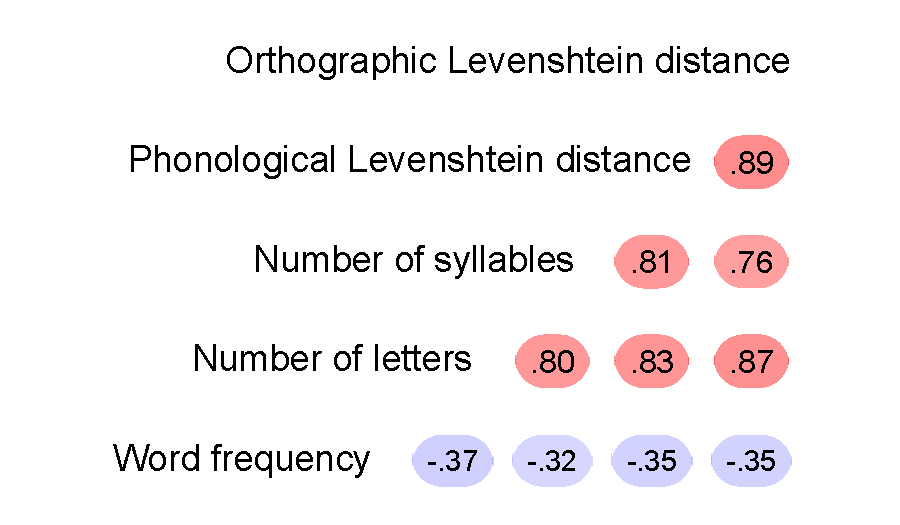
\includegraphics[width=0.5\linewidth]{manuscript_files/figure-latex/semanticpriming-lexical-covariates-correlations-1} 

}

\caption{Zero-order correlations among lexical covariates pretested in the semantic priming study.}\label{fig:semanticpriming-lexical-covariates-correlations}
\end{figure}

Table \ref{tab:semanticpriming-lexical-covariates-selection} shows the results of the selection model.

\begin{table}[!h]

\caption{\label{tab:semanticpriming-lexical-covariates-selection}Mixed-effects model for the selection of lexical covariates in the semantic priming study.}
\centering
\begin{threeparttable}
\begin{tabular}[t]{lrrrrr}
\toprule
\multicolumn{1}{c}{ } & \multicolumn{1}{c}{$\upbeta$} & \multicolumn{1}{c}{$SE$} & \multicolumn{1}{c}{95\% CI} & \multicolumn{1}{c}{$t$} & \multicolumn{1}{c}{$p$}\\
\midrule
(Intercept) & 0.01 & 0.00 & {}[0.00, 0.02] & 1.19 & .236\\
Word frequency & -0.14 & 0.01 & {}[-0.15, -0.13] & -24.19 & <.001\\
Number of letters & 0.00 & 0.01 & {}[-0.02, 0.02] & 0.12 & .903\\
Number of syllables & 0.04 & 0.01 & {}[0.02, 0.06] & 4.02 & <.001\\
Orthographic Levenshtein distance & 0.03 & 0.01 & {}[0.00, 0.05] & 2.19 & .029\\
Phonological Levenshtein distance & 0.02 & 0.01 & {}[-0.01, 0.04] & 1.28 & .199\\
\bottomrule
\end{tabular}
\begin{tablenotes}
\item \textit{\linebreak} 
\item \textit{Note}. $\upbeta$ = Estimate based on $z$-scored predictors; \textit{SE} = standard error; \linebreak \phantom{.}CI = confidence interval. By-participant random slopes were included for \linebreak \phantom{.}every effect.
\end{tablenotes}
\end{threeparttable}
\end{table}

Considering the maximum correlation allowed (\(r\) = \(\pm\).70) and the results of the model, the variables that will be included as covariates in the main analysis are word frequency and number of syllables.

\hypertarget{study-2-semantic-decision-1}{%
\subsection{Study 2: Semantic decision}\label{study-2-semantic-decision-1}}

Figure \ref{fig:semanticdecision-lexical-covariates-correlations} shows the zero-order correlations among the lexical covariates considered in the selection.

\begin{figure}

{\centering 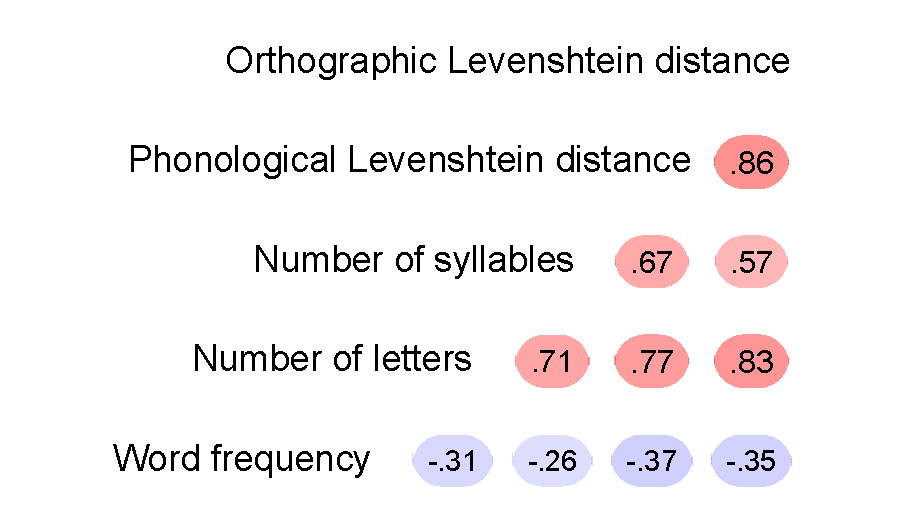
\includegraphics[width=0.5\linewidth]{manuscript_files/figure-latex/semanticdecision-lexical-covariates-correlations-1} 

}

\caption{Zero-order correlations for the lexical covariates pretested in the semantic decision study.}\label{fig:semanticdecision-lexical-covariates-correlations}
\end{figure}

Table \ref{tab:semanticdecision-lexical-covariates-selection} shows the results of the selection model.

\begin{table}[!h]

\caption{\label{tab:semanticdecision-lexical-covariates-selection}Mixed-effects model for the selection of lexical covariates in the semantic decision study.}
\centering
\begin{threeparttable}
\begin{tabular}[t]{lrrrrr}
\toprule
\multicolumn{1}{c}{ } & \multicolumn{1}{c}{$\upbeta$} & \multicolumn{1}{c}{$SE$} & \multicolumn{1}{c}{95\% CI} & \multicolumn{1}{c}{$t$} & \multicolumn{1}{c}{$p$}\\
\midrule
(Intercept) & 0.05 & 0.00 & {}[0.05, 0.06] & 12.35 & <.001\\
Word frequency & -0.13 & 0.01 & {}[-0.14, -0.11] & -20.01 & <.001\\
Number of letters & 0.05 & 0.01 & {}[0.03, 0.07] & 5.20 & <.001\\
Number of syllables & 0.08 & 0.01 & {}[0.07, 0.10] & 10.80 & <.001\\
Orthographic Levenshtein distance & -0.13 & 0.01 & {}[-0.15, -0.10] & -10.23 & <.001\\
Phonological Levenshtein distance & 0.01 & 0.01 & {}[-0.01, 0.03] & 0.91 & .361\\
\bottomrule
\end{tabular}
\begin{tablenotes}
\item \textit{\linebreak} 
\item \textit{Note}. $\upbeta$ = Estimate based on $z$-scored predictors; \textit{SE} = standard error; \linebreak \phantom{.}CI = confidence interval. By-participant random slopes were included for \linebreak \phantom{.}every effect.
\end{tablenotes}
\end{threeparttable}
\end{table}

Considering the maximum correlation allowed (\(r\) = \(\pm\).70) and the results of the model, the variables that will be included as covariates in the main analysis are word frequency and orthographic Levenshtein distance.

\hypertarget{study-3-lexical-decision}{%
\subsection{Study 3: Lexical decision}\label{study-3-lexical-decision}}

The selection model for Study 3 served a twofold purpose. First, the variable that had the largest effect out of the five was selected as the language-based predictor of interest (see reason in \protect\hyperlink{lexicaldecision}{\underline{Study 3 in the main text}}). Second, one variable was selected as a covariate among the remaining four.

Figure \ref{fig:lexicaldecision-lexical-covariates-correlations} shows the zero-order correlations among the lexical covariates considered in the selection.

\begin{figure}

{\centering 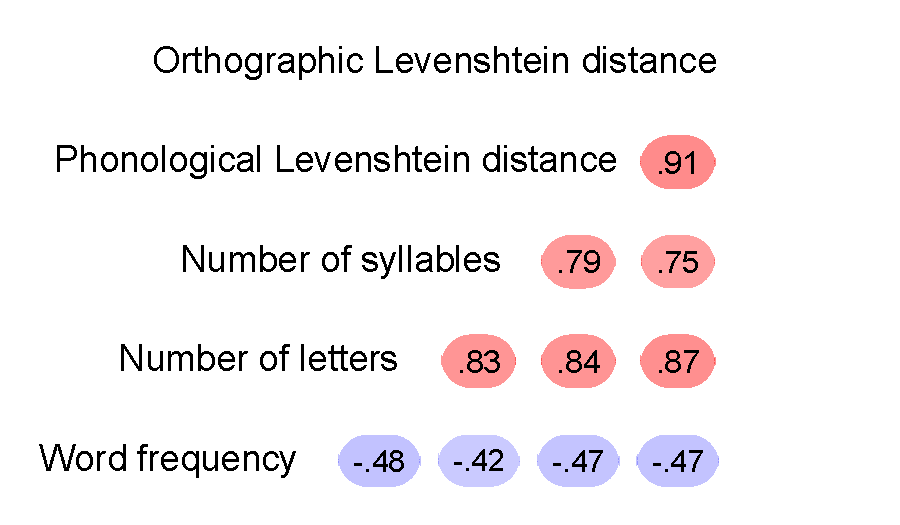
\includegraphics[width=0.5\linewidth]{manuscript_files/figure-latex/lexicaldecision-lexical-covariates-correlations-1} 

}

\caption{Zero-order correlations for the lexical covariates pretested in the lexical decision study.}\label{fig:lexicaldecision-lexical-covariates-correlations}
\end{figure}

Table \ref{tab:lexicaldecision-lexical-covariates-selection} shows the results of the selection model.

\begin{table}[!h]

\caption{\label{tab:lexicaldecision-lexical-covariates-selection}Mixed-effects model for the selection of lexical covariates in the lexical decision study.}
\centering
\begin{threeparttable}
\begin{tabular}[t]{lrrrrr}
\toprule
\multicolumn{1}{c}{ } & \multicolumn{1}{c}{$\upbeta$} & \multicolumn{1}{c}{$SE$} & \multicolumn{1}{c}{95\% CI} & \multicolumn{1}{c}{$t$} & \multicolumn{1}{c}{$p$}\\
\midrule
(Intercept) & 0.00 & 0.01 & {}[-0.01, 0.01] & -0.02 & .981\\
Word frequency & -0.12 & 0.01 & {}[-0.15, -0.10] & -11.60 & <.001\\
Number of letters & 0.05 & 0.02 & {}[0.01, 0.09] & 2.73 & .006\\
Number of syllables & 0.06 & 0.01 & {}[0.03, 0.09] & 4.43 & <.001\\
Orthographic Levenshtein distance & 0.10 & 0.02 & {}[0.05, 0.14] & 4.52 & <.001\\
Phonological Levenshtein distance & -0.02 & 0.02 & {}[-0.06, 0.02] & -1.18 & .238\\
\bottomrule
\end{tabular}
\begin{tablenotes}
\item \textit{\linebreak} 
\item \textit{Note}. $\upbeta$ = Estimate based on $z$-scored predictors; \textit{SE} = standard error; \linebreak \phantom{.}CI = confidence interval. By-participant random slopes were included for \linebreak \phantom{.}every effect.
\end{tablenotes}
\end{threeparttable}
\end{table}

Considering the maximum correlation allowed (\(r\) = \(\pm\).70), the results of the model, and the use of word frequency as a predictor of interest in the model, the variable that will be included as a covariate in the main analysis is orthographic Levenshtein distance.

\hypertarget{conclusion}{%
\subsection{Conclusion}\label{conclusion}}

Word frequency presented the largest effect in the three models. Orthographic Levenshtein distance was the second largest effect in the semantic decision and the lexical decision studies, whereas its phonological counterpart was not significant in any of the studies. The latter difference makes sense, as participants read the stimulus words in the three studies (Brysbaert, 2022).

\clearpage

\renewcommand{\thefigure}{B\arabic{figure}} \setcounter{figure}{0}
\renewcommand{\thetable}{B\arabic{table}} \setcounter{table}{0}

\hypertarget{appendix-B-frequentist-analysis-diagnostics}{%
\section{Appendix B: Diagnostics for the frequentist analyses}\label{appendix-B-frequentist-analysis-diagnostics}}

Below, the convergence warnings and the non-normal residuals are first addressed generally, and then in more detail in the context of each study.

\hypertarget{convergence-1}{%
\subsection{Convergence}\label{convergence-1}}

The challenge of convergence is well known in the area of mixed-effects models. These models often struggle to reach reliable-enough estimates due to an insufficiency of data relative to the complexity of the model (Baayen et al., 2008; Bates et al., 2015; Brauer \& Curtin, 2018). The solutions proposed range from the removal of random slopes under certain conditions (Matuschek et al., 2017) to the maintenance of random slopes in spite of convergence warnings, which seeks to avoid an inflation of the Type I error due to dependencies in the data (Brauer \& Curtin, 2018; Singmann \& Kellen, 2019).

\hypertarget{the-multiple-optimisers-sanity-check-from-lme4allfit}{%
\subsubsection{\texorpdfstring{The multiple-optimisers sanity check from \texttt{lme4::allFit()}}{The multiple-optimisers sanity check from lme4::allFit()}}\label{the-multiple-optimisers-sanity-check-from-lme4allfit}}

Framed within the drive to maintain random slopes wherever possible, the developers of the `lme4' package propose a sanity check that uses a part of the `lme4' \emph{engine} called `optimiser'. Every model has a default optimiser, unless a specific one is chosen through \texttt{control\ =\ lmerControl(optimiser\ =\ \textquotesingle{}...\textquotesingle{})} (in \texttt{lmer} models) or \texttt{control\ =\ glmerControl(optimiser\ =\ \textquotesingle{}...\textquotesingle{})} (in \texttt{glmer} models). The seven widely-available optimisers are:

\begin{itemize}
\tightlist
\item
  bobyqa
\item
  Nelder\_Mead
\item
  nlminbwrap
\item
  nmkbw
\item
  optimx.L-BFGS-B
\item
  nloptwrap.NLOPT\_LN\_NELDERMEAD
\item
  nloptwrap.NLOPT\_LN\_BOBYQA
\end{itemize}

To assess whether convergence warnings render the results invalid, or on the contrary, the results can be deemed valid in spite of the warnings, Bates et al. (2021) suggest refitting models affected by convergence warnings with a variety of optimisers. The authors argue that if the different optimisers produce practically-equivalent results, the results are valid. For this purpose, the `allFit' function from the `lme4' package allows the refitting of models using a number of optimisers. To use the seven optimisers listed above, two extra packages were installed: `dfoptim' and `optimx' (see \href{https://cran.r-project.org/web/packages/lme4/lme4.pdf}{lme4 manual}). The output from `allFit' contains several statistics on the fixed and the random effects fitted by each optimiser (see \href{https://github.com/lme4/lme4/issues/512\#issue-425198940}{example}).

The severity of convergence problems in each study will be examined below using the `allFit' function from the `lme4' package.

\hypertarget{residual-errors-not-normally-distributed}{%
\subsection{Residual errors not normally distributed}\label{residual-errors-not-normally-distributed}}

The residuals of the linear mixed-effects models in the three studies violated the assumption of normality. Even though linear mixed-effects models tend to be quite robust to deviations from normality (Knief \& Forstmeier, 2021; Schielzeth et al., 2020), we sought to verify our results. To this end, we attempted to run robust models using two methods, neither of which worked. The methods are nonetheless described below.

\hypertarget{method-a-robustlmm-model}{%
\subsubsection{\texorpdfstring{Method A: \emph{robustlmm} model}{Method A: robustlmm model}}\label{method-a-robustlmm-model}}

The first method drew on the R package `robustlmm' v2.4-4 (Koller, 2016). To calculate the \(p\) values, we followed the procedure of Sleegers et al. (2021), but used the Kenward-Roger method instead of Satterthwaite (see Luke, 2017).

\hypertarget{method-b-inverse-gaussian-model-with-identity-link-function}{%
\subsubsection{Method B: Inverse Gaussian model with identity link function}\label{method-b-inverse-gaussian-model-with-identity-link-function}}

In the second approach, we followed a method proposed by Lo and Andrews (2015), based on generalized linear mixed-effects models (GLMM) implementing an identity link function. According to Lo and Andrews (2015), the link function helps avoid directly transforming the dependent variable, which can hinder the interpretability of the results (also see Knief \& Forstmeier, 2021).

GLMMs require the use of families of distributions. Lo and Andrews (2015) tested the Gaussian, Gamma and Inverse Gaussian families, with either an identity or an inverse link function. The authors found that the Inverse Gaussian family with an identity link yielded the most normal residuals. The Inverse Gaussian and the Gamma families only accept positive values in the outcome variable (see Table 15.2 in Fox, 2016). Due to this restriction, the dependent variable in the present model is raw RT, unlike the standardised RT that was used in the main analysis.

\(P\) values were to be calculated through parametric bootstrapping, which is the most robust method for GLMMs, as the Kenward-Roger and Satterthwaite methods are not available for these models (Luke, 2017; Singmann et al., 2021).

Neither Method A nor Method B could finally be used, as the code produced errors. These errors are shown in the corresponding scripts inside the `model\_diagnostics' folder in each study.

The residuals of the final models are shown in the corresponding sections below.

\hypertarget{study-1-semantic-priming-2}{%
\subsection{Study 1: Semantic priming}\label{study-1-semantic-priming-2}}

\hypertarget{convergence-2}{%
\subsubsection{Convergence}\label{convergence-2}}

In the initial model, the optimiser used (the default one in `lmerTest') was '`, and the convergence warning read: 'boundary (singular) fit: see ?isSingular'.

Based on the reanalysis using seven optimisers, Figure \ref{fig:main-effects-semanticpriming-allFit-convergence} shows the fixed, main effects, and Figure \ref{fig:interactions-semanticpriming-allFit-convergence} shows the fixed interactions.

\begin{figure}

{\centering 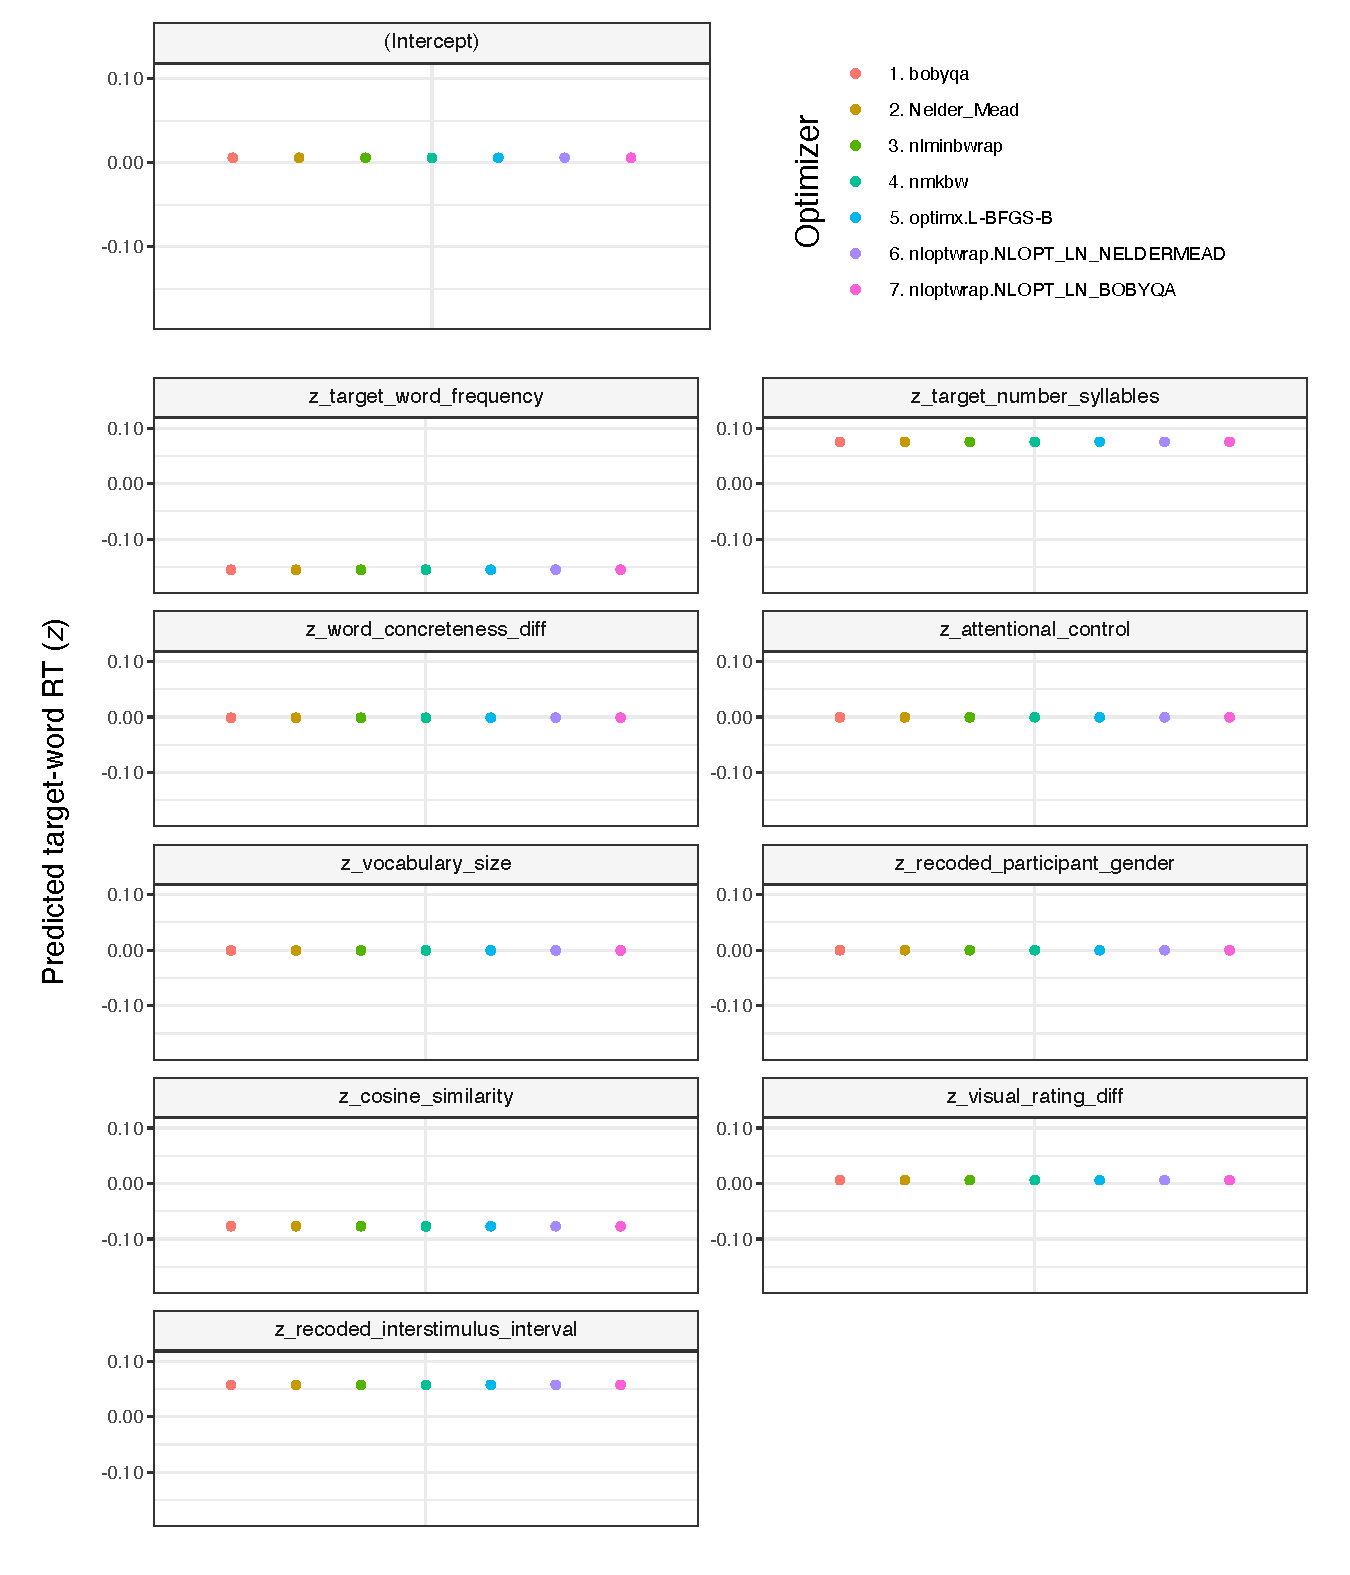
\includegraphics[width=1\linewidth]{C:/Users/Pablo/Documents/semanticpriming-semanticdecision-lexicaldecision/semanticpriming/frequentist_analysis/model_diagnostics/plots/main_effects_semanticpriming_allFit_convergence} 

}

\caption{Fixed, main effects from the semantic priming study fitted by seven optimisers.}\label{fig:main-effects-semanticpriming-allFit-convergence}
\end{figure}

\begin{figure}

{\centering 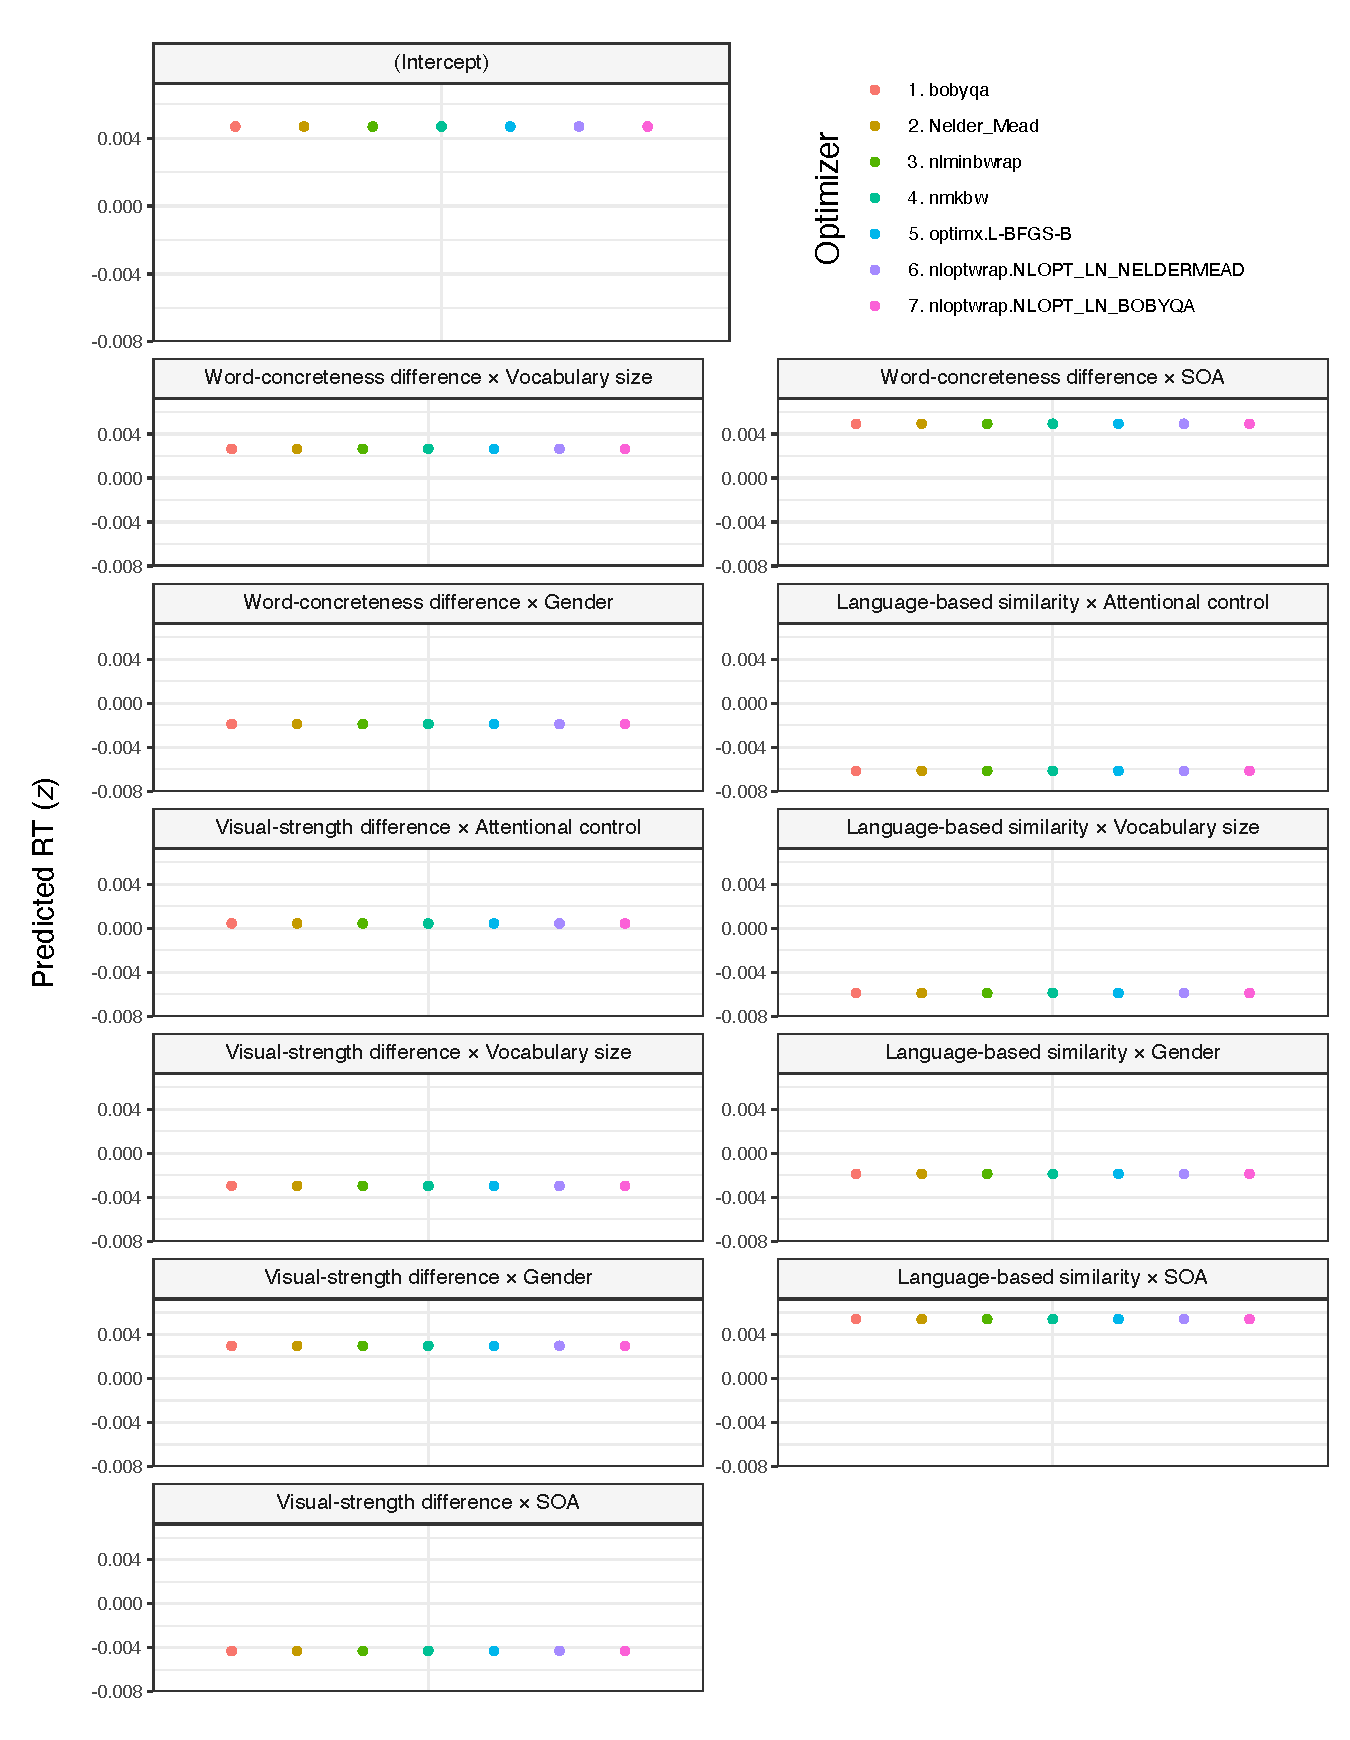
\includegraphics[width=1\linewidth]{C:/Users/Pablo/Documents/semanticpriming-semanticdecision-lexicaldecision/semanticpriming/frequentist_analysis/model_diagnostics/plots/interactions_semanticpriming_allFit_convergence} 

}

\caption{Fixed interaction effects from the semantic priming study fitted by seven optimisers.}\label{fig:interactions-semanticpriming-allFit-convergence}
\end{figure}

\hypertarget{residual-errors-not-normally-distributed-1}{%
\subsubsection{Residual errors not normally distributed}\label{residual-errors-not-normally-distributed-1}}

Figure \ref{fig:semanticpriming-residuals} shows the deviation from normality of the residuals of the linear mixed-effects model.

\begin{figure}

{\centering 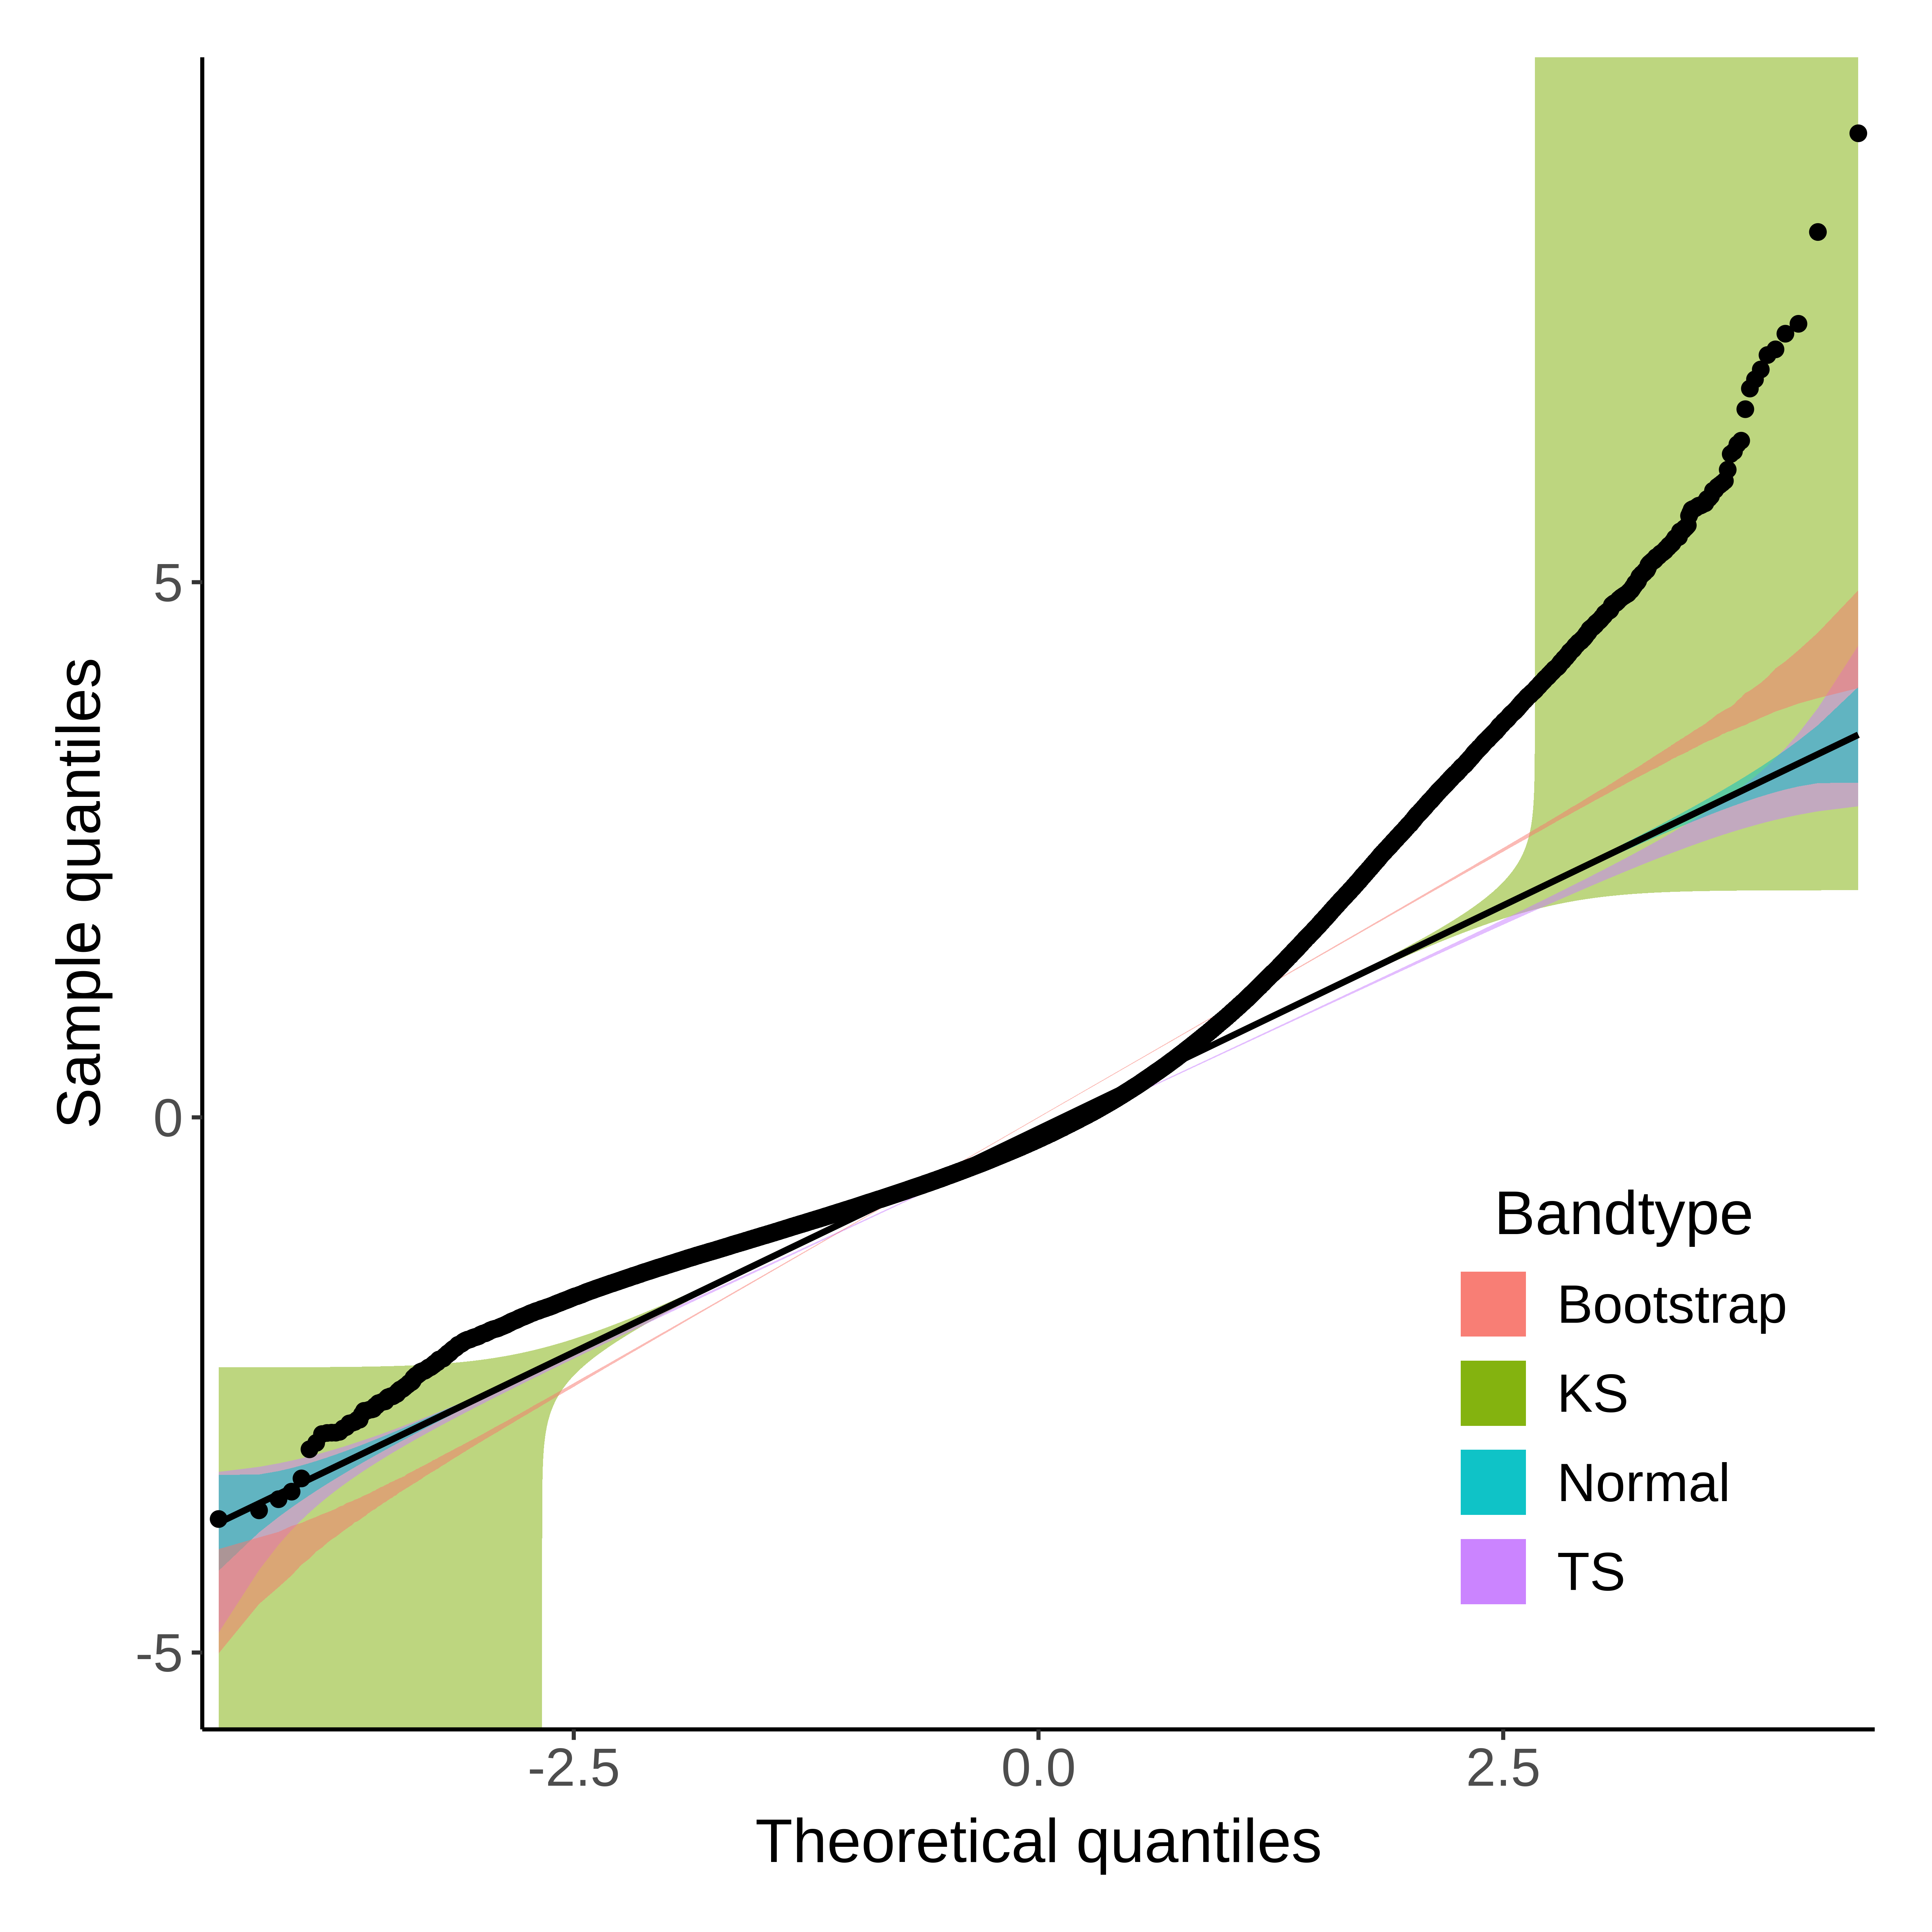
\includegraphics[width=0.65\linewidth]{C:/Users/Pablo/Documents/semanticpriming-semanticdecision-lexicaldecision/semanticpriming/frequentist_analysis/model_diagnostics/plots/semanticpriming_residuals} 

}

\caption{Residuals of the linear mixed-effects model from the semantic priming study. \linebreak KS = Kolmogorov-Smirnov test; TS = tail-sensitive confidence bands.}\label{fig:semanticpriming-residuals}
\end{figure}

\hypertarget{semantic-priming-model-including-visual-similarity}{%
\subsubsection{Semantic priming model including visual similarity}\label{semantic-priming-model-including-visual-similarity}}

\hypertarget{convergence-3}{%
\paragraph{Convergence}\label{convergence-3}}

In the initial model, the optimiser used (the default one in `lmerTest') was '`, and the convergence warning read: 'boundary (singular) fit: see ?isSingular'.

Based on the reanalysis using seven optimisers, Figure \ref{fig:main-effects-semanticpriming-with-visualsimilarity-allFit-convergence} shows the fixed, main effects, and Figure \ref{fig:interactions-semanticpriming-with-visualsimilarity-allFit-convergence} shows the fixed interactions.

\begin{figure}

{\centering 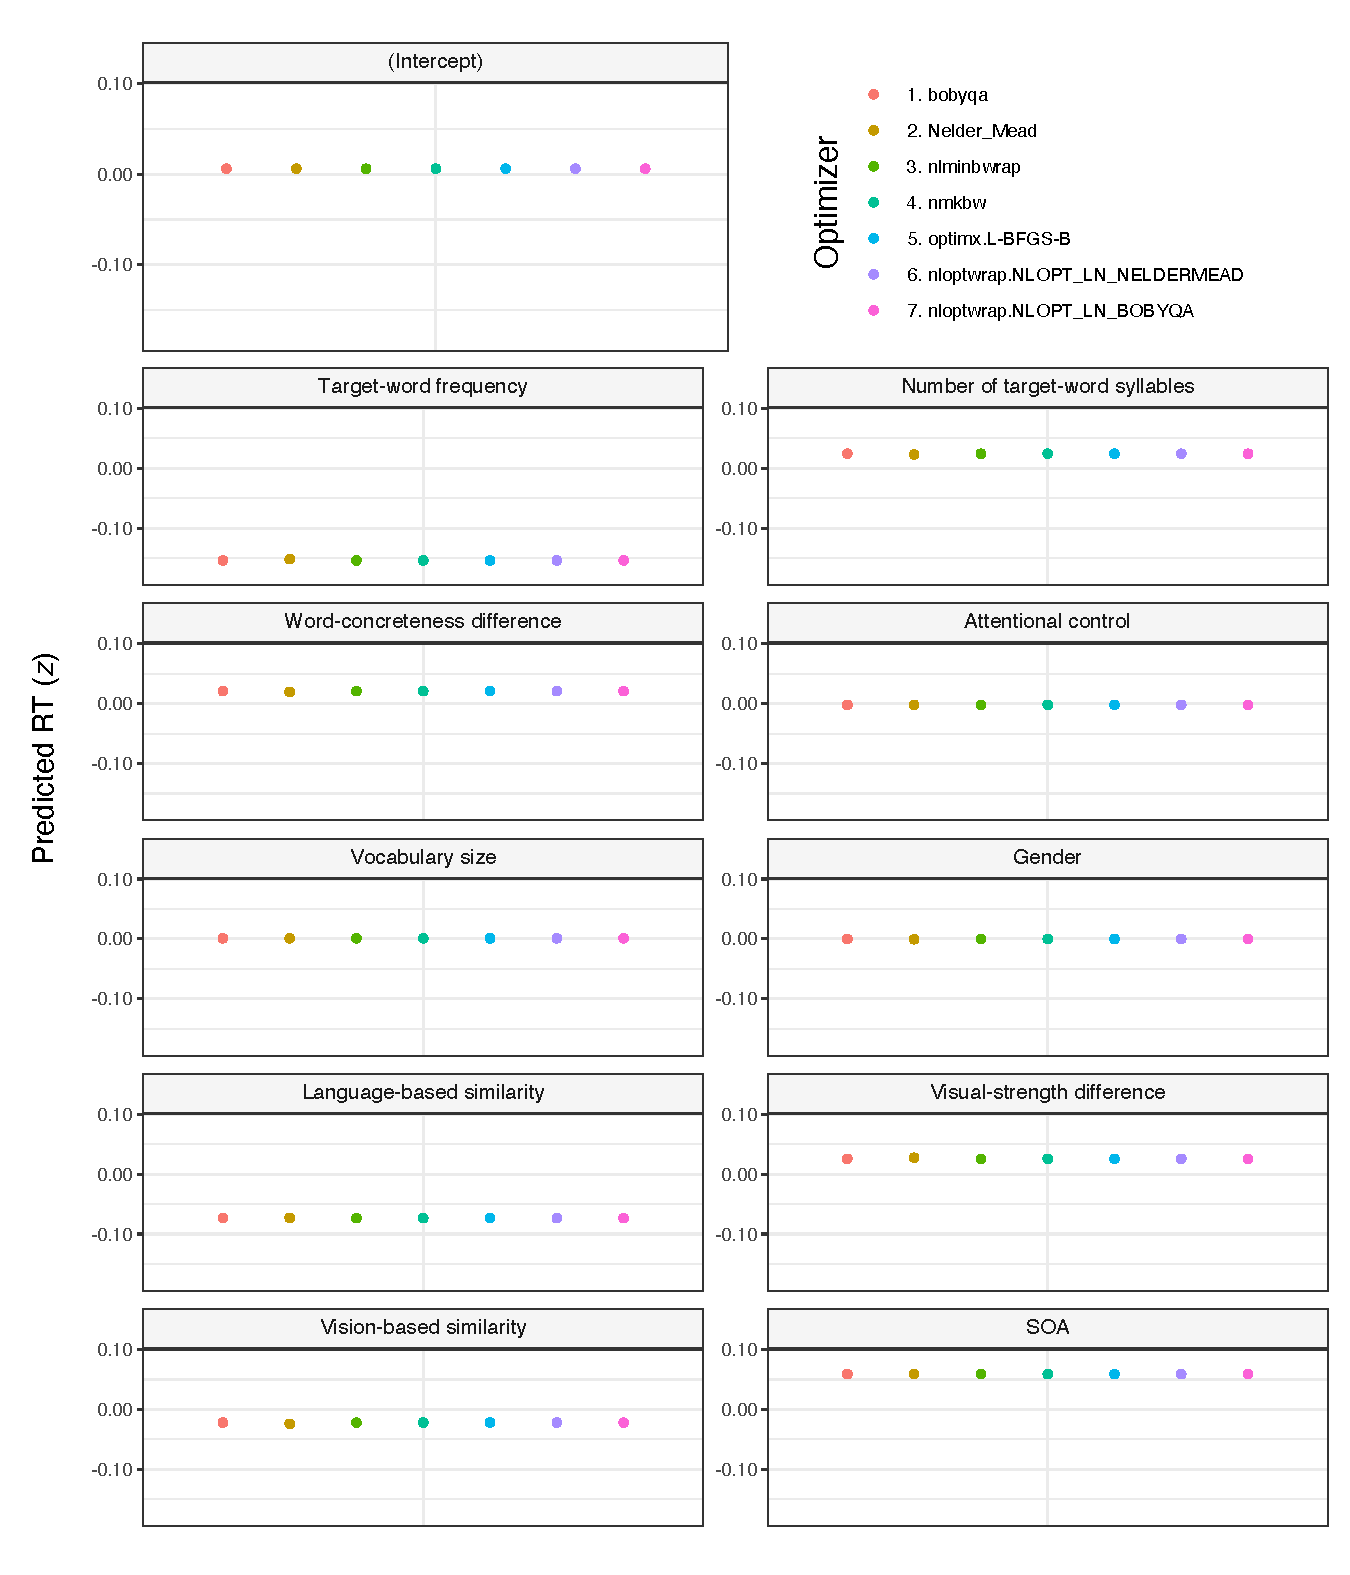
\includegraphics[width=1\linewidth]{C:/Users/Pablo/Documents/semanticpriming-semanticdecision-lexicaldecision/semanticpriming/analysis_with_visualsimilarity/model_diagnostics/plots/main_effects_semanticpriming_with_visualsimilarity_allFit_convergence} 

}

\caption{Fixed, main effects from the semantic priming study fitted by seven optimisers.}\label{fig:main-effects-semanticpriming-with-visualsimilarity-allFit-convergence}
\end{figure}

\begin{figure}

{\centering 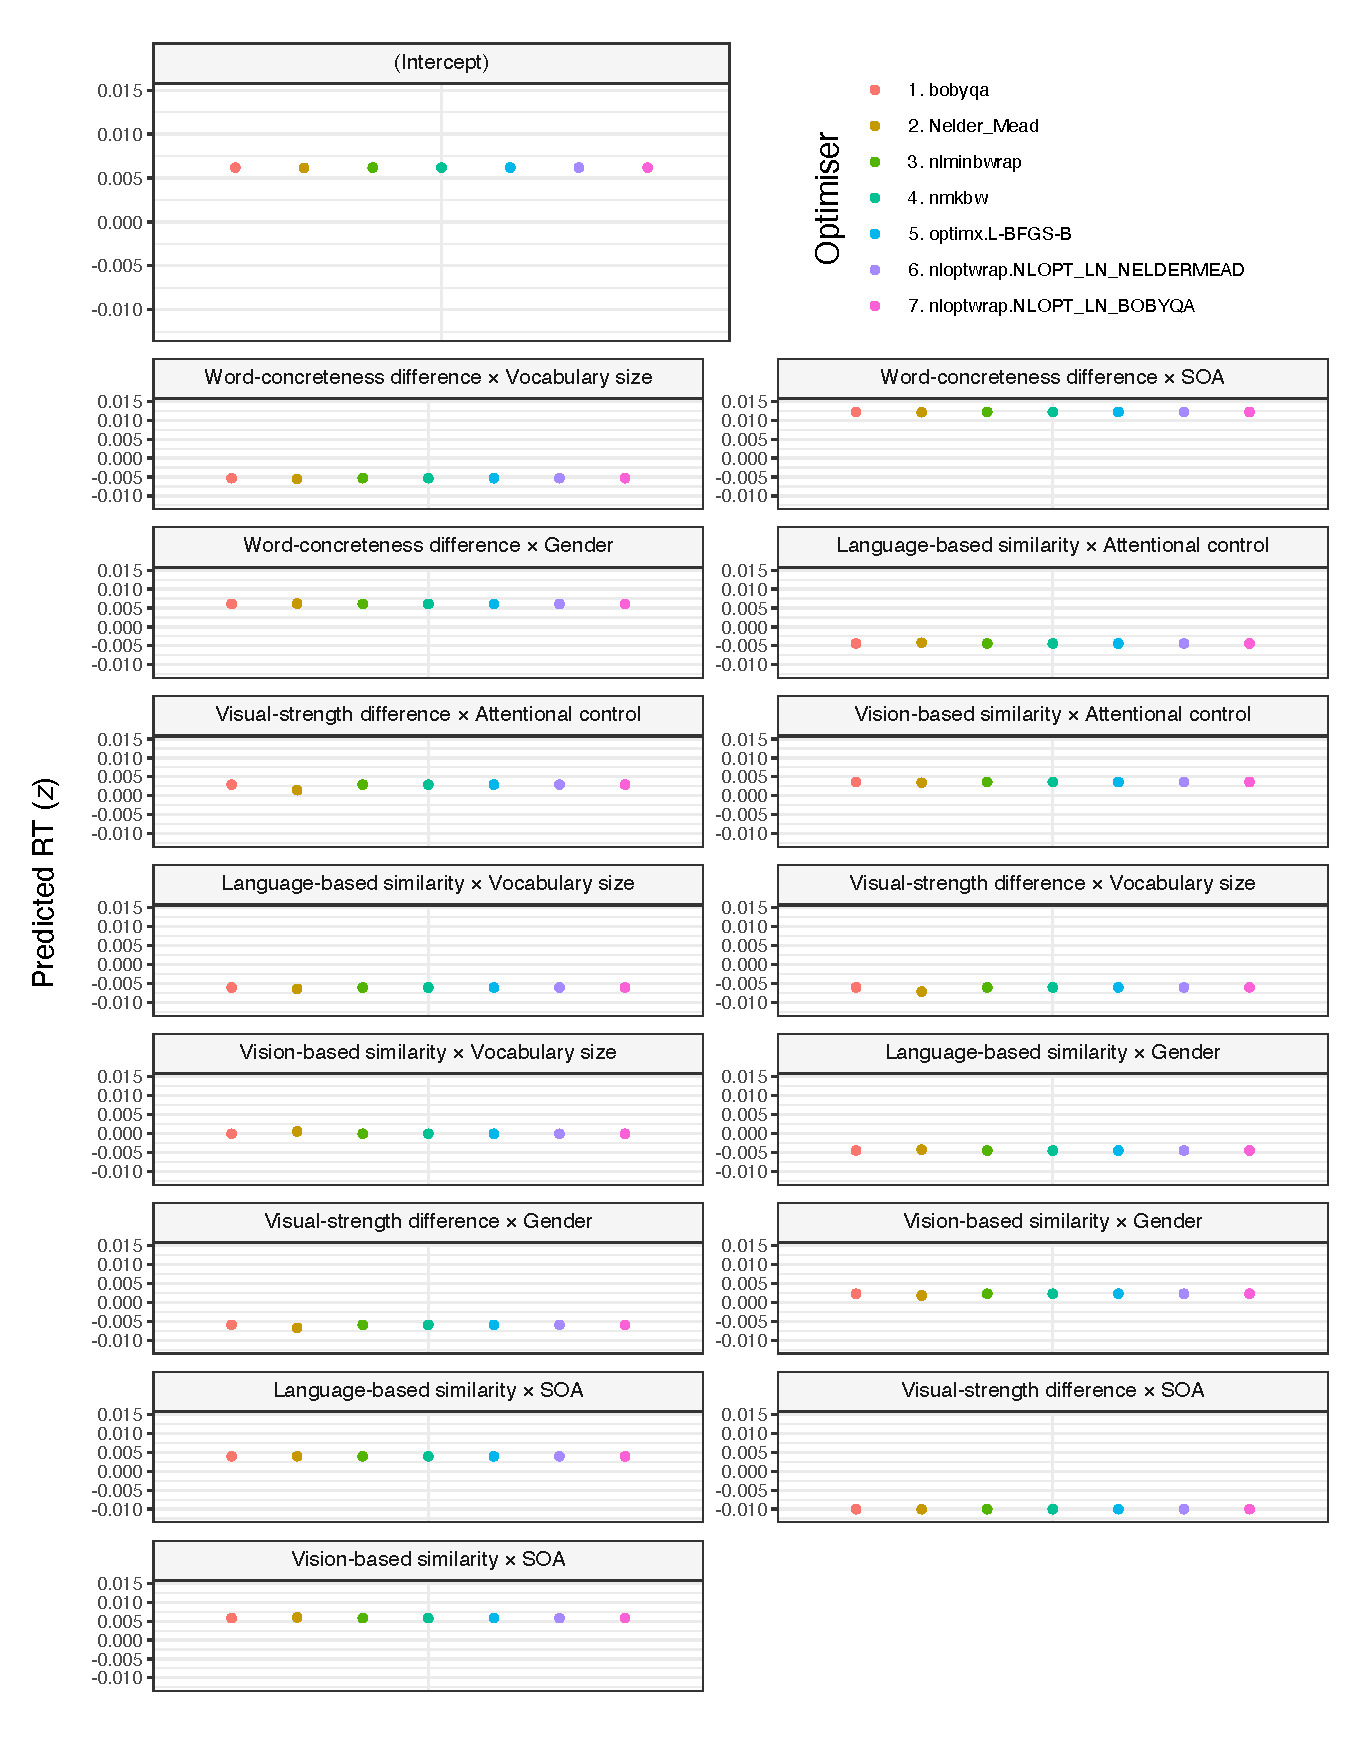
\includegraphics[width=1\linewidth]{C:/Users/Pablo/Documents/semanticpriming-semanticdecision-lexicaldecision/semanticpriming/analysis_with_visualsimilarity/model_diagnostics/plots/interactions_semanticpriming_with_visualsimilarity_allFit_convergence} 

}

\caption{Fixed interaction effects from the semantic priming study fitted by seven optimisers.}\label{fig:interactions-semanticpriming-with-visualsimilarity-allFit-convergence}
\end{figure}

\hypertarget{residual-errors-not-normally-distributed-2}{%
\paragraph{Residual errors not normally distributed}\label{residual-errors-not-normally-distributed-2}}

Figure \ref{fig:semanticpriming-with-visualsimilarity-residuals} shows the deviation from normality of the residuals of the linear mixed-effects model.

\begin{figure}

{\centering 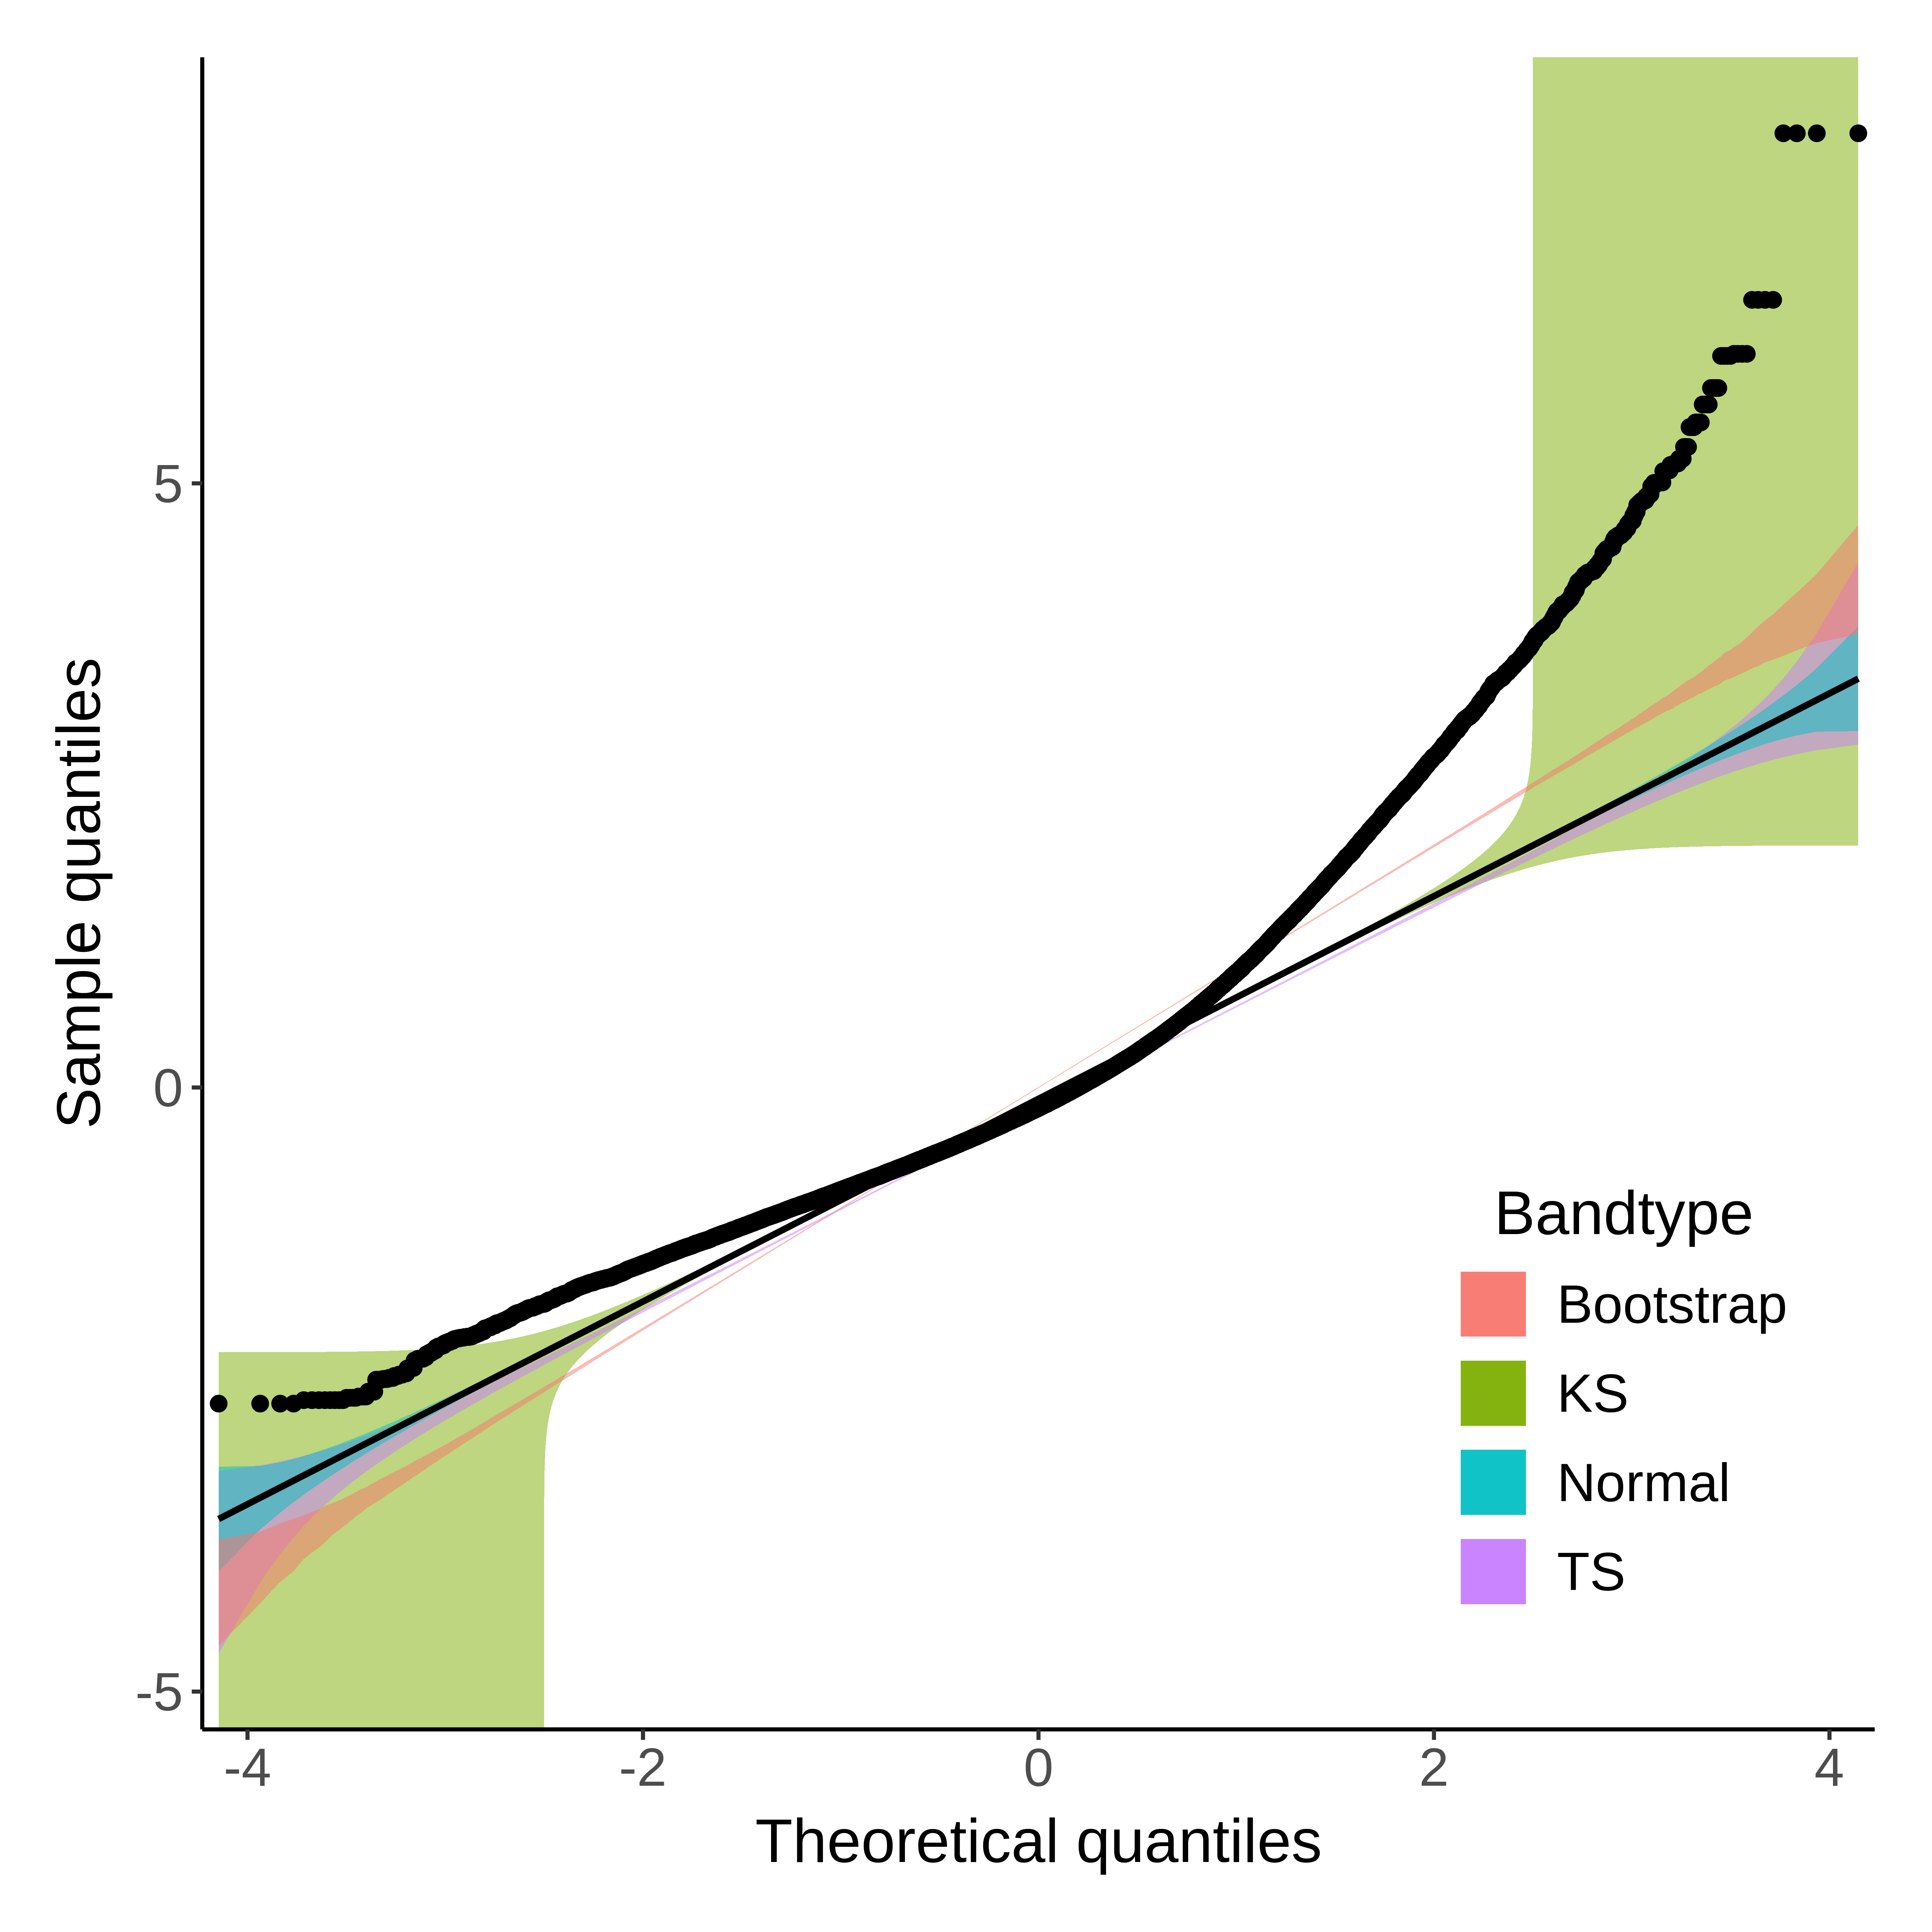
\includegraphics[width=0.65\linewidth]{C:/Users/Pablo/Documents/semanticpriming-semanticdecision-lexicaldecision/semanticpriming/analysis_with_visualsimilarity/model_diagnostics/plots/semanticpriming_with_visualsimilarity_residuals} 

}

\caption{Residuals of the linear mixed-effects model from the semantic priming study. \linebreak KS = Kolmogorov-Smirnov test; TS = tail-sensitive confidence bands.}\label{fig:semanticpriming-with-visualsimilarity-residuals}
\end{figure}

\hypertarget{study-2-semantic-decision-2}{%
\subsection{Study 2: Semantic decision}\label{study-2-semantic-decision-2}}

\hypertarget{convergence-4}{%
\subsubsection{Convergence}\label{convergence-4}}

In the initial model, the optimiser used (the default one in `lmerTest') was '`, and the convergence warning read: 'boundary (singular) fit: see ?isSingular'.

Based on the reanalysis using seven optimisers, Figure \ref{fig:main-effects-semanticdecision-allFit-convergence} shows the fixed, main effects, and Figure \ref{fig:interactions-semanticdecision-allFit-convergence} shows the fixed interactions.

\begin{figure}

{\centering 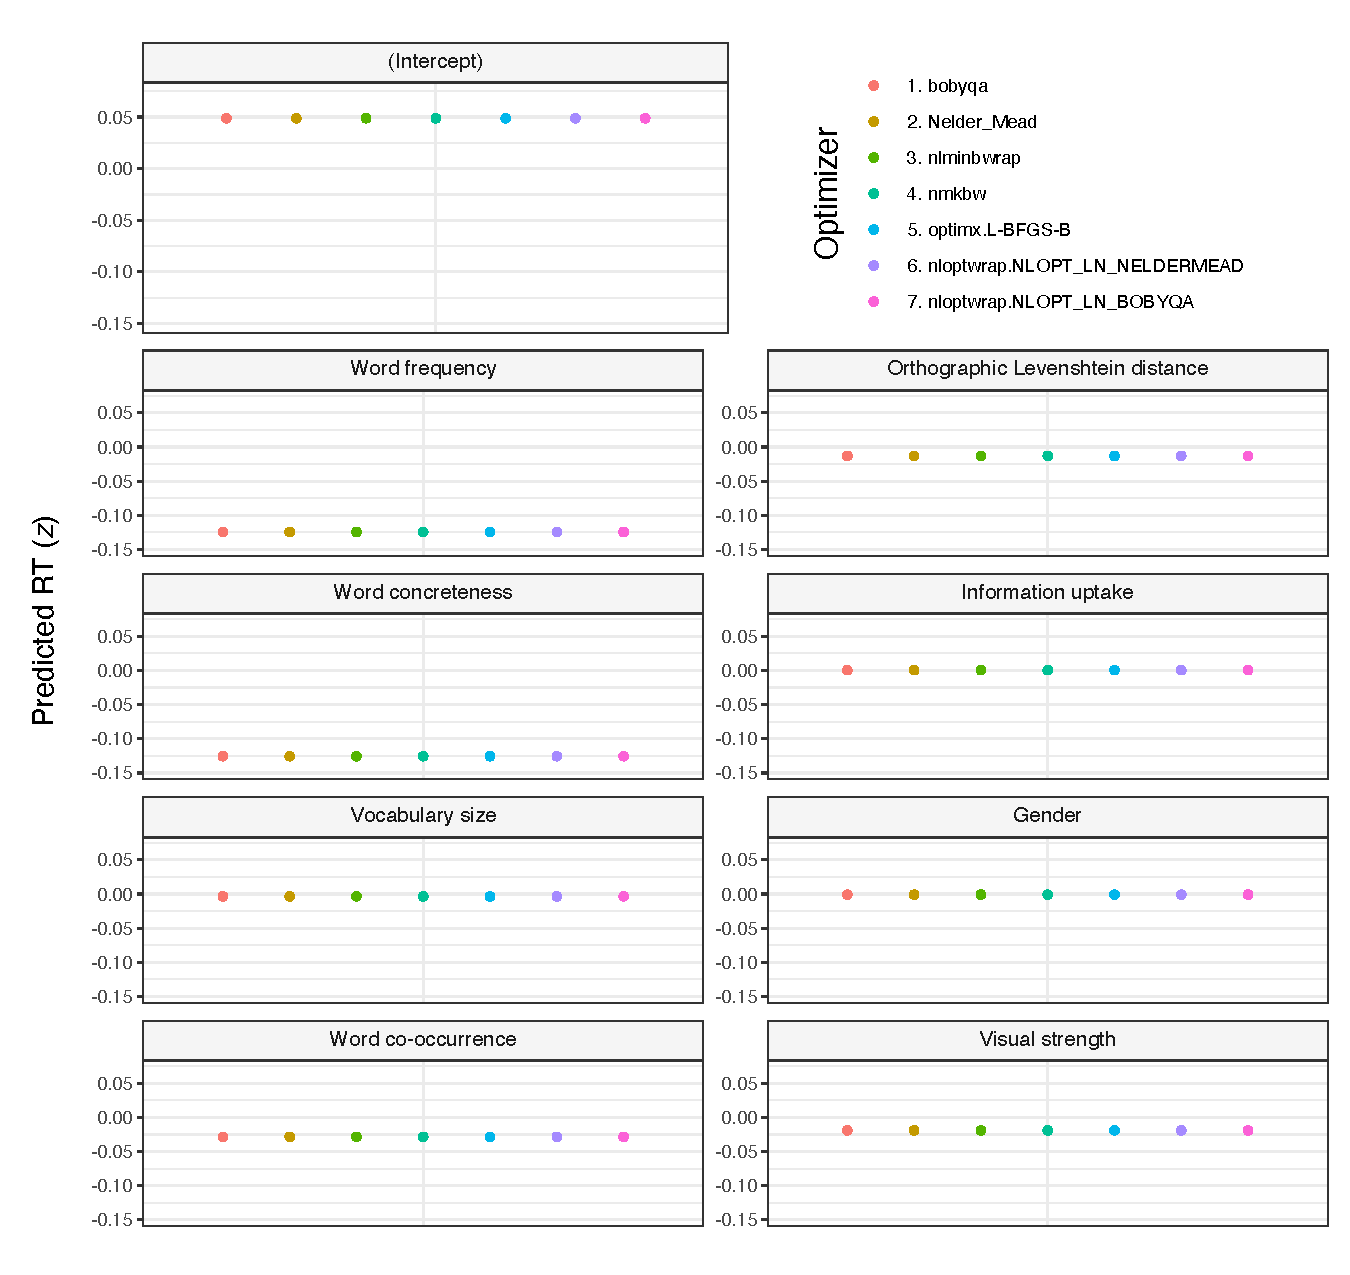
\includegraphics[width=1\linewidth]{C:/Users/Pablo/Documents/semanticpriming-semanticdecision-lexicaldecision/semanticdecision/frequentist_analysis/model_diagnostics/plots/main_effects_semanticdecision_allFit_convergence} 

}

\caption{Fixed, main effects from the semantic decision study fitted by seven optimisers.}\label{fig:main-effects-semanticdecision-allFit-convergence}
\end{figure}

\begin{figure}

{\centering 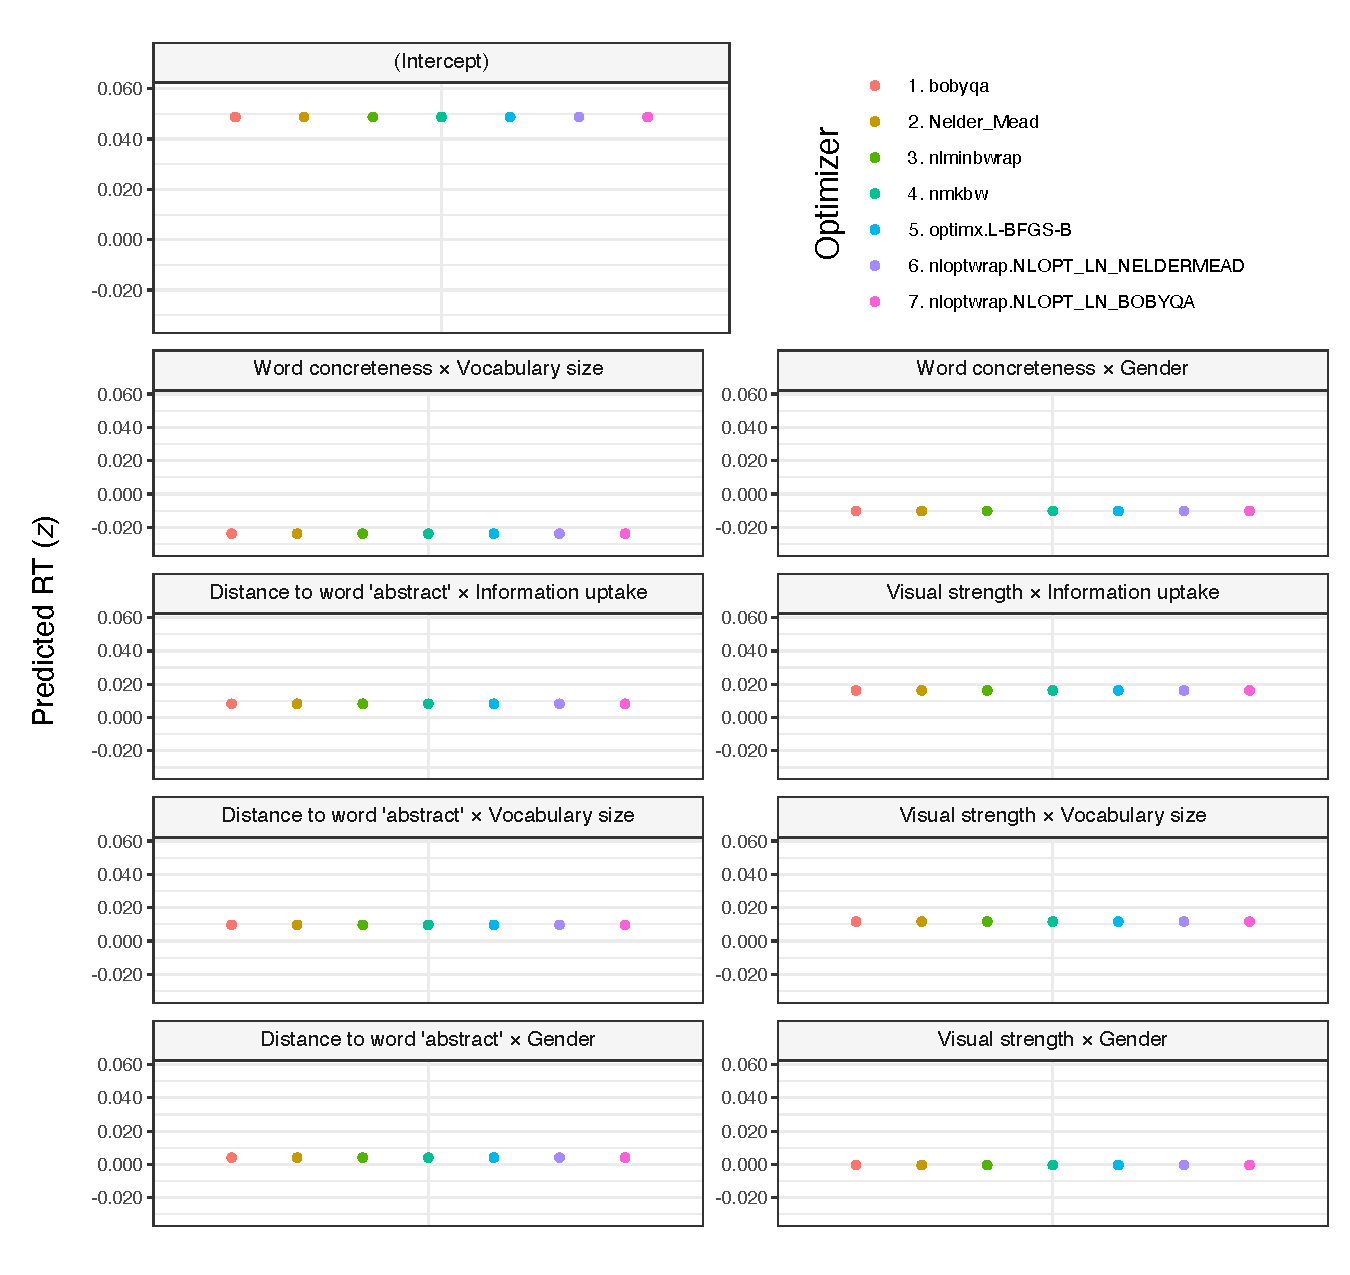
\includegraphics[width=1\linewidth]{C:/Users/Pablo/Documents/semanticpriming-semanticdecision-lexicaldecision/semanticdecision/frequentist_analysis/model_diagnostics/plots/interactions_semanticdecision_allFit_convergence} 

}

\caption{Fixed interaction effects from the semantic decision study fitted by seven optimisers.}\label{fig:interactions-semanticdecision-allFit-convergence}
\end{figure}

\hypertarget{residual-errors-not-normally-distributed-3}{%
\subsubsection{Residual errors not normally distributed}\label{residual-errors-not-normally-distributed-3}}

Figure \ref{fig:semanticdecision-residuals} shows the deviation from normality of the residuals.

\begin{figure}

{\centering 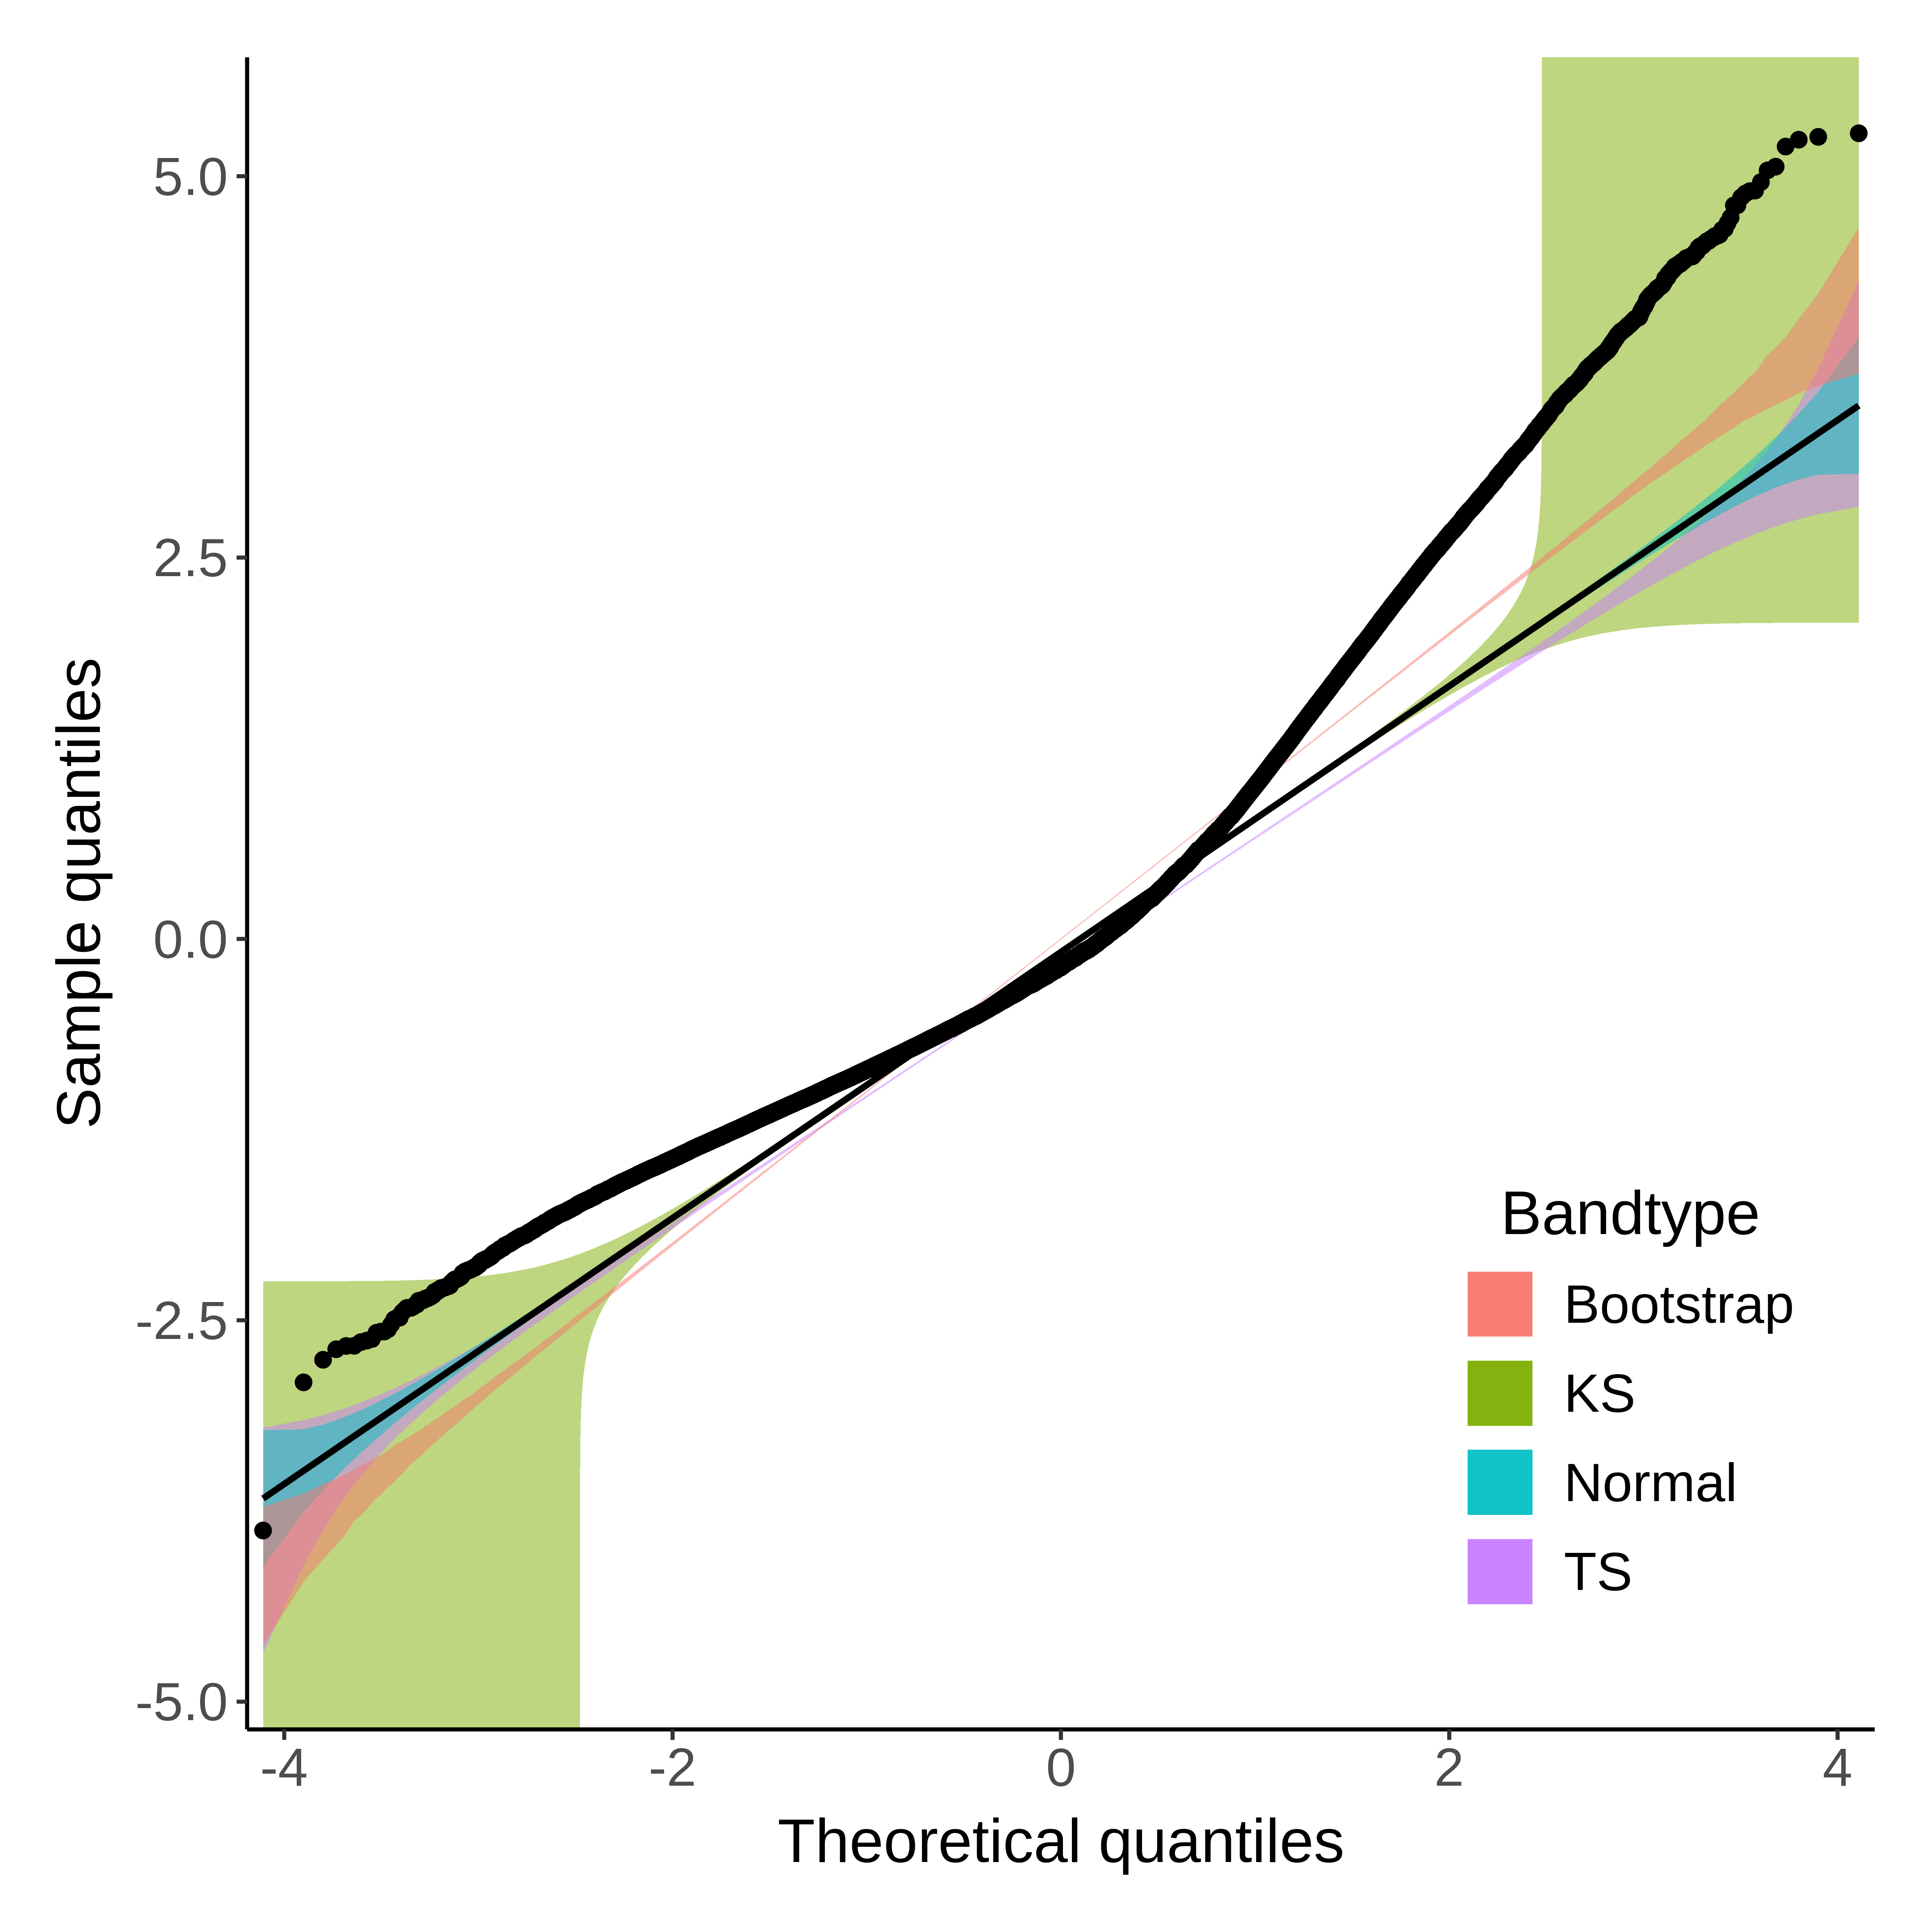
\includegraphics[width=0.65\linewidth]{C:/Users/Pablo/Documents/semanticpriming-semanticdecision-lexicaldecision/semanticdecision/frequentist_analysis/model_diagnostics/plots/semanticdecision_residuals} 

}

\caption{Residuals of the linear mixed-effects model from the semantic decision study. \linebreak KS = Kolmogorov-Smirnov test; TS = tail-sensitive confidence bands.}\label{fig:semanticdecision-residuals}
\end{figure}

\hypertarget{study-3-lexical-decision-1}{%
\subsection{Study 3: Lexical decision}\label{study-3-lexical-decision-1}}

\hypertarget{convergence-5}{%
\subsubsection{Convergence}\label{convergence-5}}

In the initial model, the optimiser used (the default one in `lmerTest') was '`, and the convergence warning read: 'boundary (singular) fit: see ?isSingular'.

Based on the reanalysis using seven optimisers, Figure \ref{fig:main-effects-lexicaldecision-allFit-convergence} shows the fixed, main effects, and Figure \ref{fig:interactions-lexicaldecision-allFit-convergence} shows the fixed interactions.

\begin{figure}

{\centering 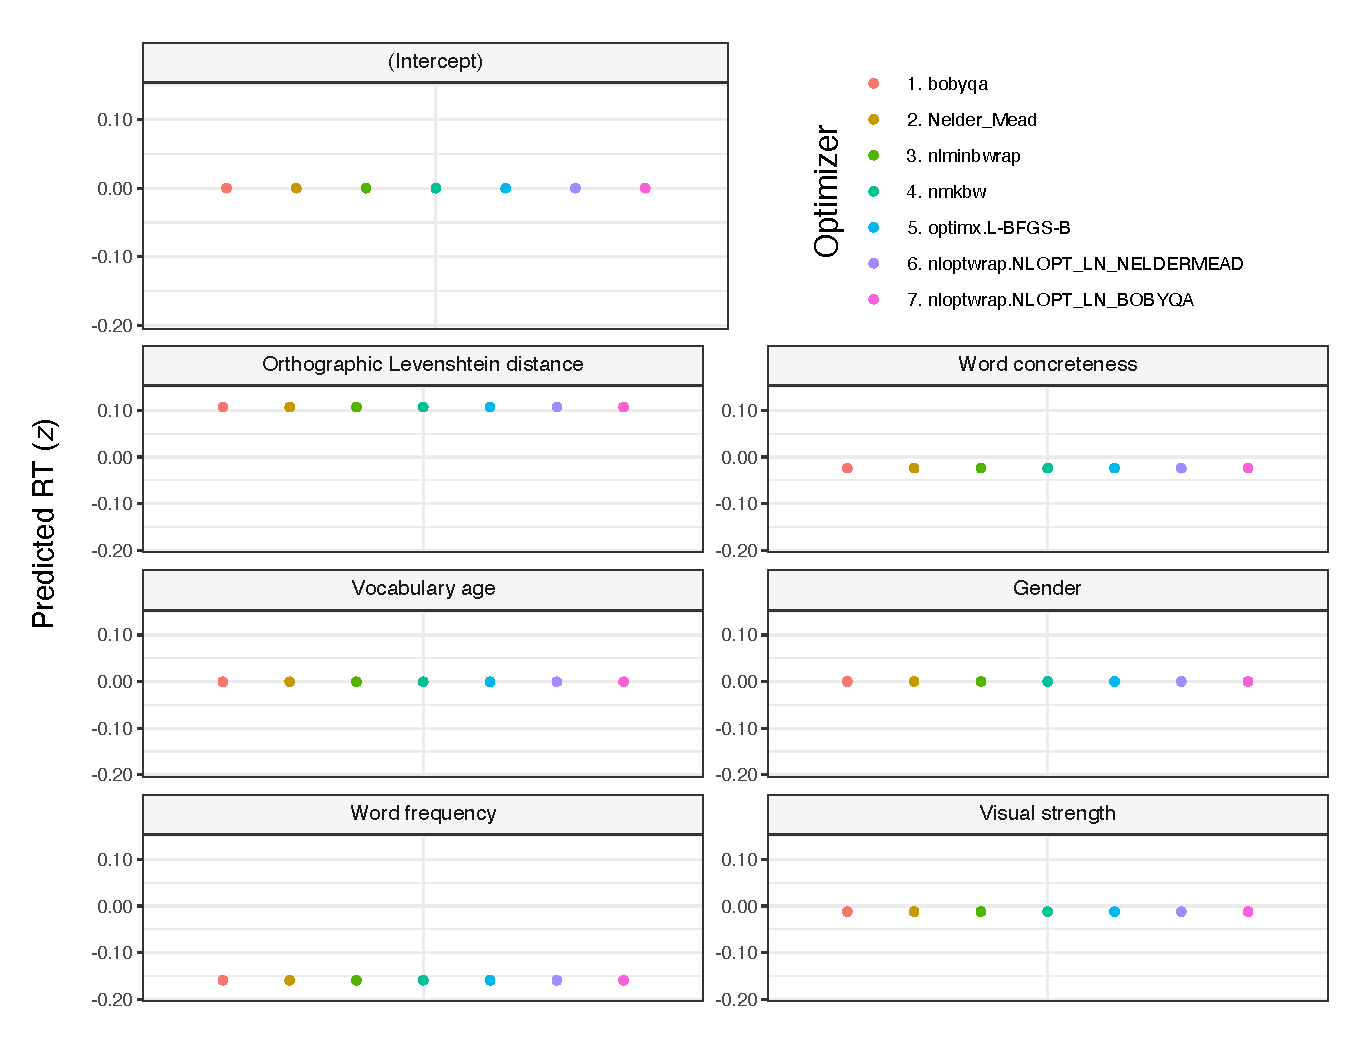
\includegraphics[width=1\linewidth]{C:/Users/Pablo/Documents/semanticpriming-semanticdecision-lexicaldecision/lexicaldecision/frequentist_analysis/model_diagnostics/plots/main_effects_lexicaldecision_allFit_convergence} 

}

\caption{Fixed, main effects from the lexical decision study fitted by seven optimisers.}\label{fig:main-effects-lexicaldecision-allFit-convergence}
\end{figure}

\begin{figure}

{\centering 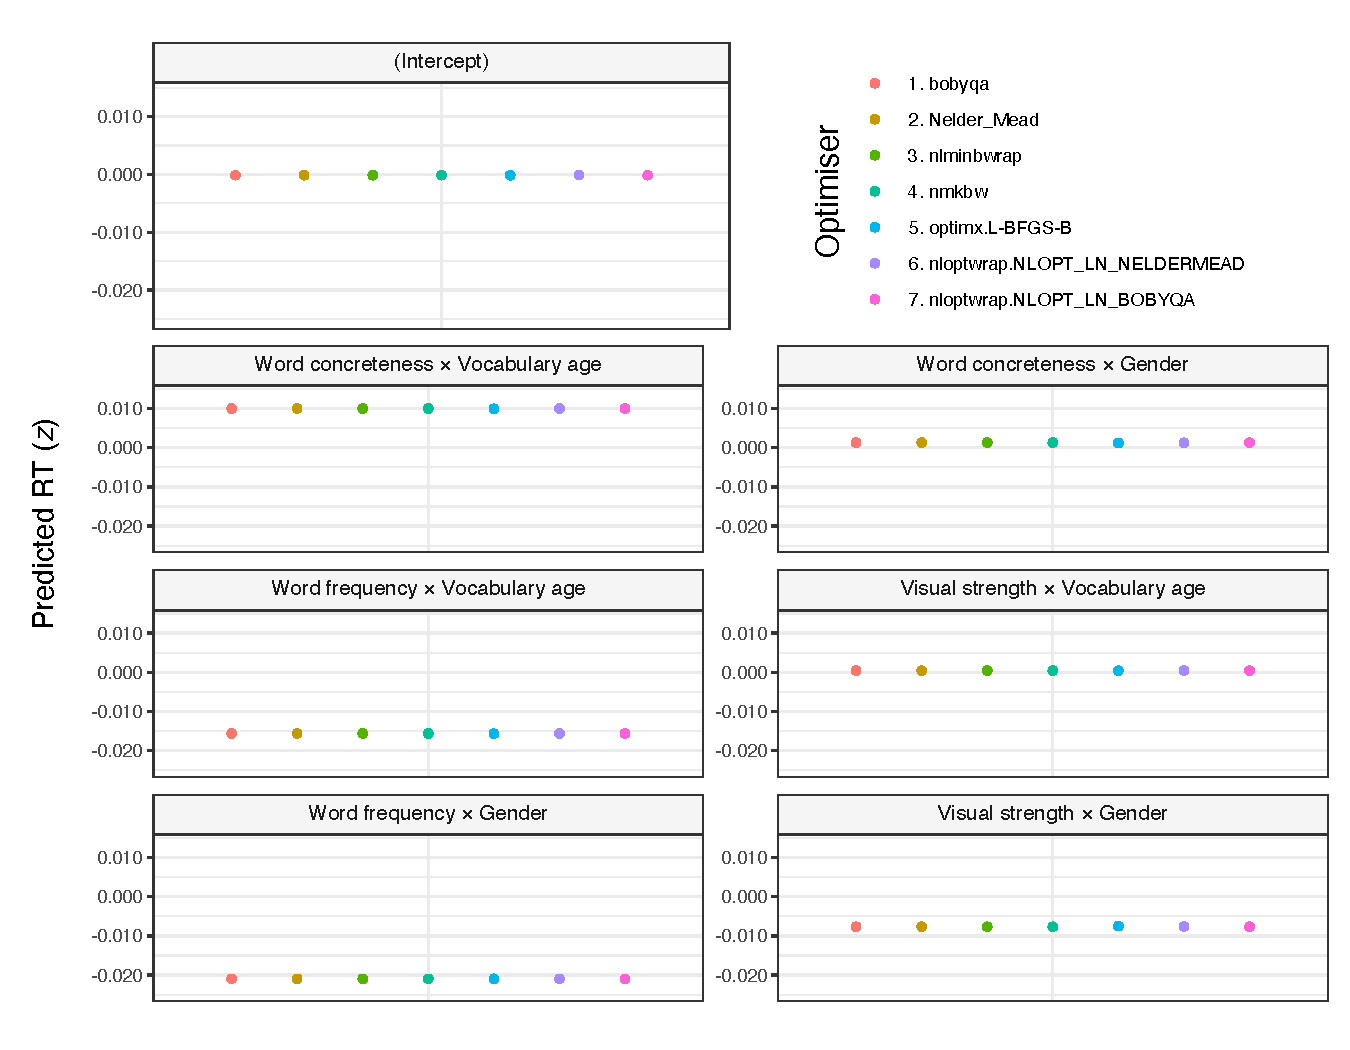
\includegraphics[width=1\linewidth]{C:/Users/Pablo/Documents/semanticpriming-semanticdecision-lexicaldecision/lexicaldecision/frequentist_analysis/model_diagnostics/plots/interactions_lexicaldecision_allFit_convergence} 

}

\caption{Fixed interaction effects from the lexical decision study fitted by seven optimisers.}\label{fig:interactions-lexicaldecision-allFit-convergence}
\end{figure}

\hypertarget{residual-errors-not-normally-distributed-4}{%
\subsubsection{Residual errors not normally distributed}\label{residual-errors-not-normally-distributed-4}}

Figure \ref{fig:lexicaldecision-residuals} shows the deviation from normality of the residuals.

\begin{figure}

{\centering 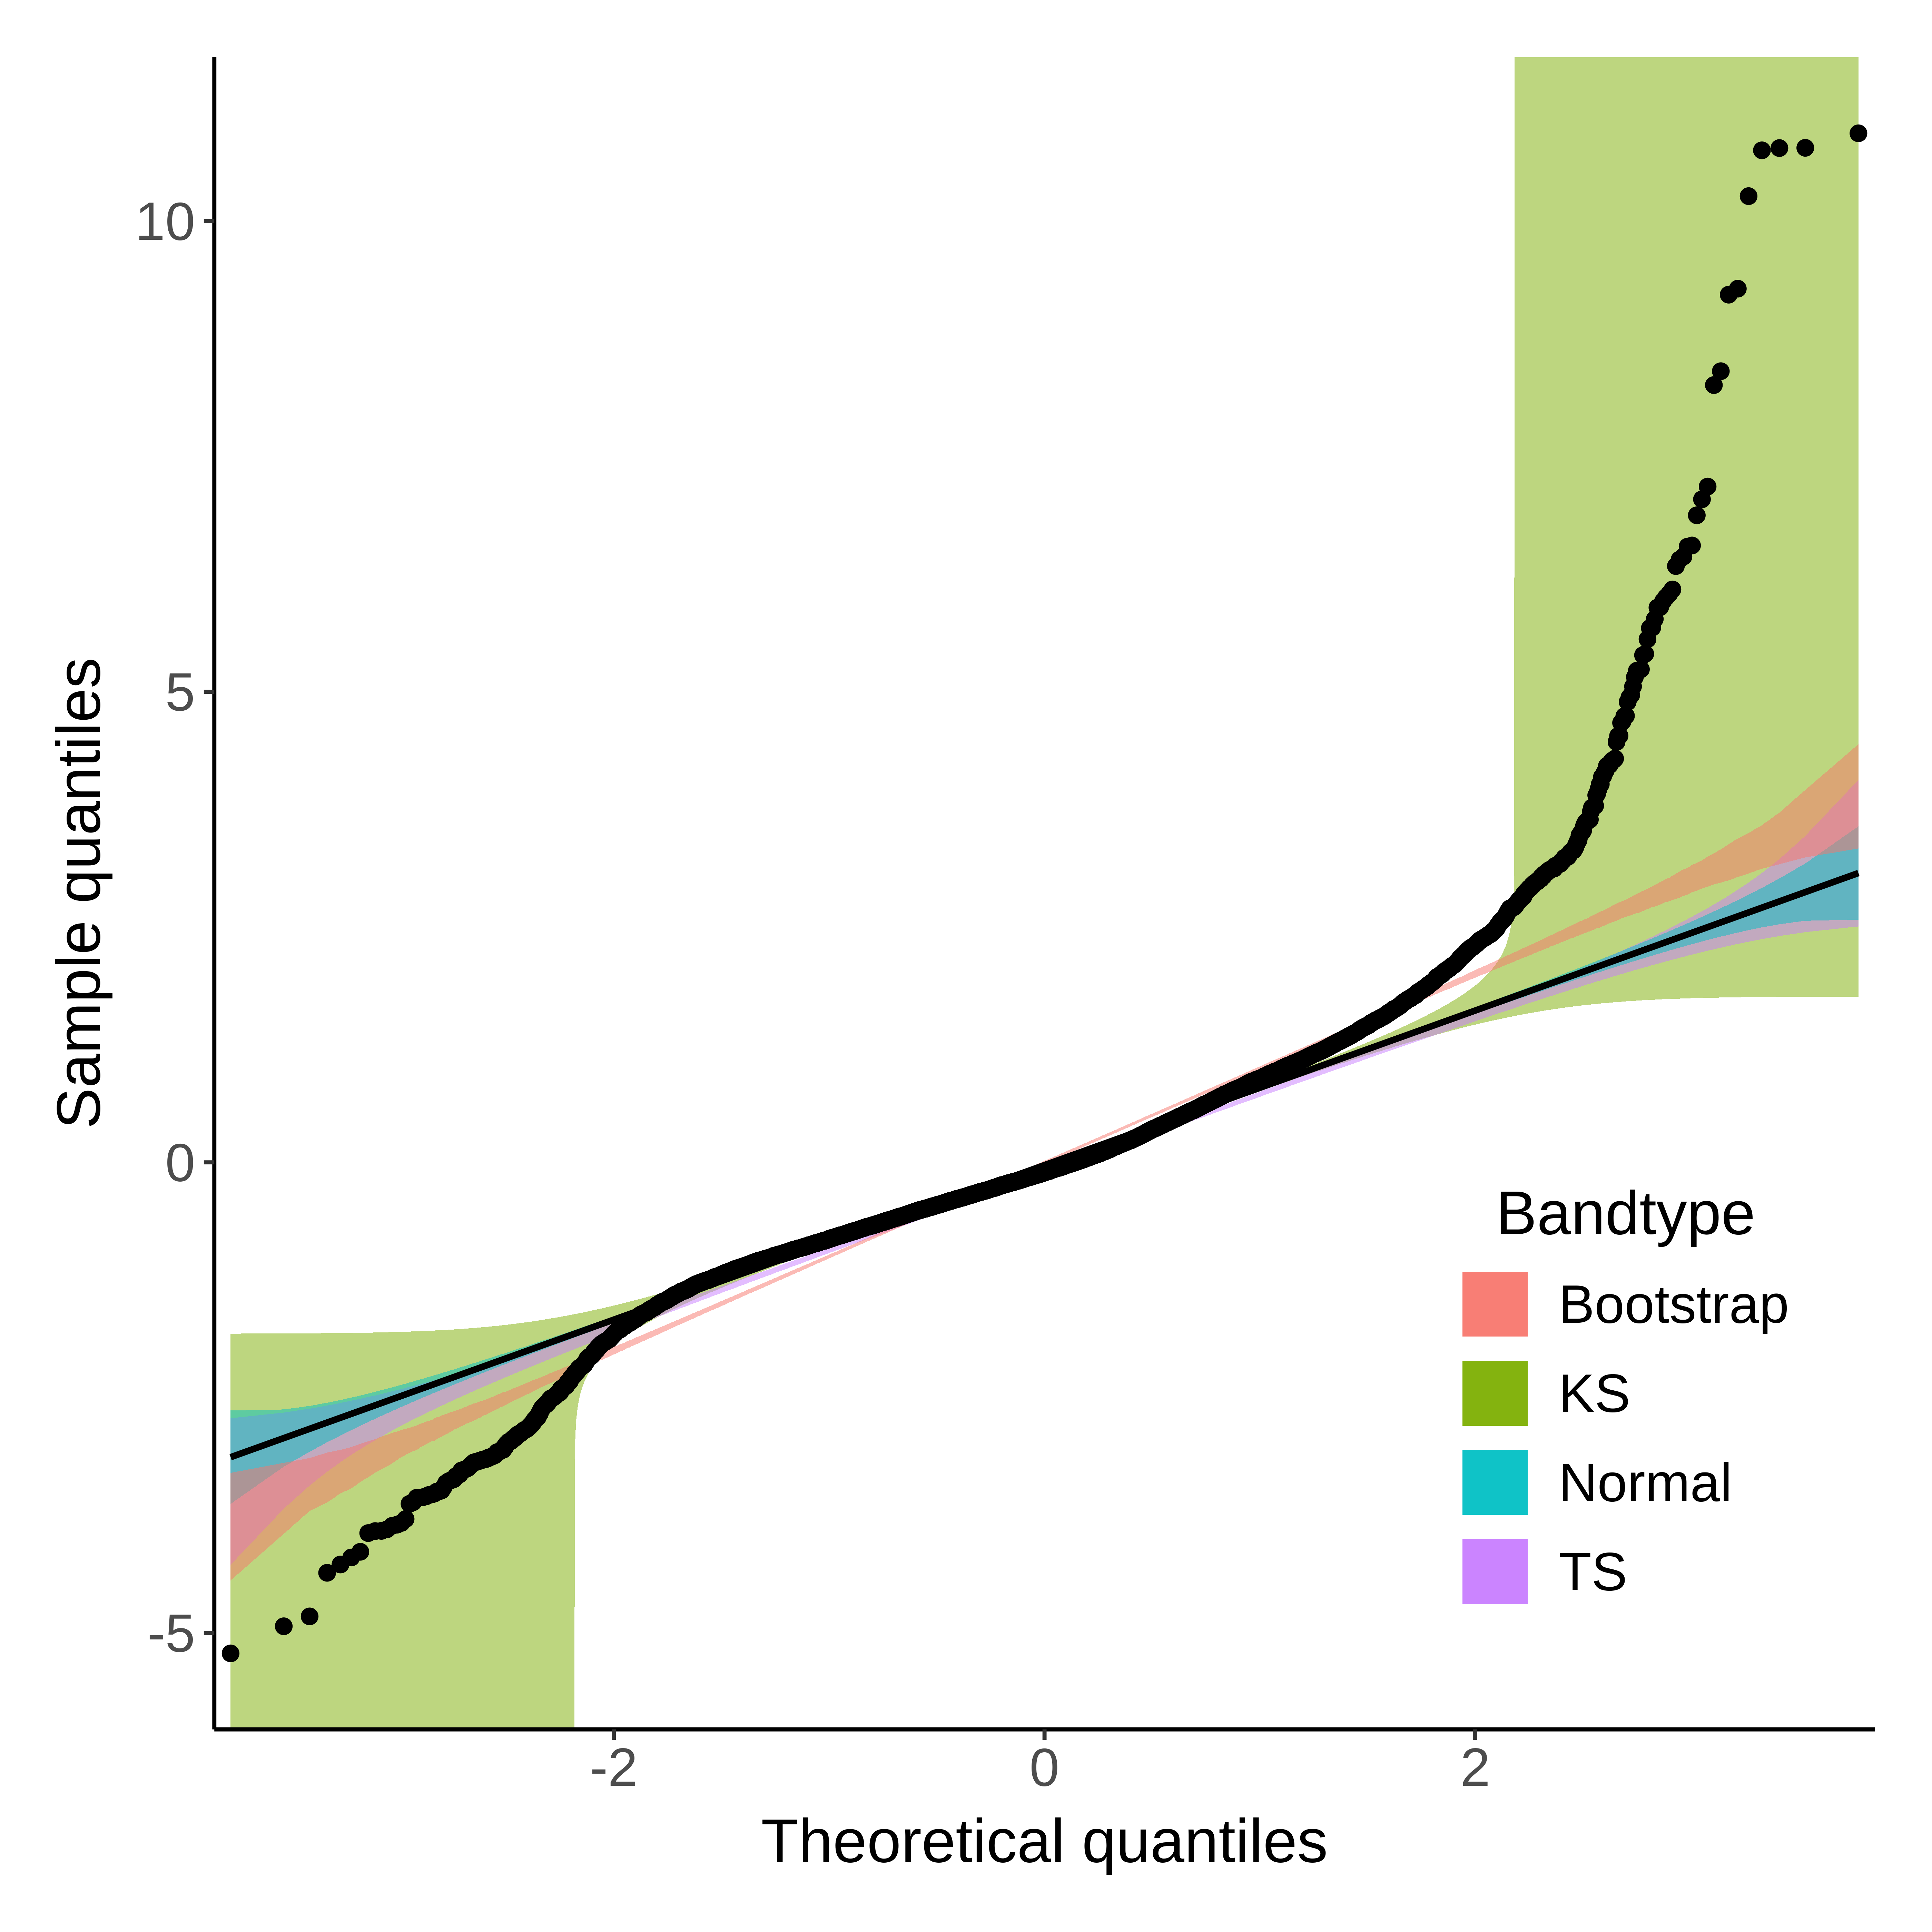
\includegraphics[width=0.65\linewidth]{C:/Users/Pablo/Documents/semanticpriming-semanticdecision-lexicaldecision/lexicaldecision/frequentist_analysis/model_diagnostics/plots/lexicaldecision_residuals} 

}

\caption{Residuals of the linear mixed-effects model from the lexical decision study. The outliers in the residuals deviate from the coloured areas indicating an acceptable normality. \linebreak KS = Kolmogorov-Smirnov test; TS = tail-sensitive confidence bands.}\label{fig:lexicaldecision-residuals}
\end{figure}

\clearpage

\renewcommand{\thefigure}{C\arabic{figure}} \setcounter{figure}{0}
\renewcommand{\thetable}{C\arabic{table}} \setcounter{table}{0}

\hypertarget{appendix-C-Bayesian-analysis-diagnostics}{%
\section{Appendix C: Diagnostics for the Bayesian analyses}\label{appendix-C-Bayesian-analysis-diagnostics}}

This appendix presents diagnostics for the Bayesian analyses. In each study, prior predictive checks are presented before posterior predictive checks. Furthermore, in each of these checks, the models presented first have the default Gaussian distribution, whereas the next series have an exponentially modified Gaussian (dubbed `ex-Gaussian') distribution with an identity link function (for details, see the section titled `Distributions and prior predictive checks' in the main text). Eyeball estimation is used to assess the outcomes of these checks (for background on predictive checks and for alternative estimation procedures, see Gelman et al., 1996; Moran et al., 2022; Schoot et al., 2021). One diagnostic not shown in this appendix is the \(\widehat R\), which is shown in \protect\hyperlink{appendix-E-Bayesian-analysis-results}{\underline{Appendix E}} instead.

\hypertarget{study1-bayesian-diagnostics}{%
\subsection{Study 1: Semantic priming}\label{study1-bayesian-diagnostics}}

\hypertarget{prior-predictive-checks}{%
\subsubsection{Prior predictive checks}\label{prior-predictive-checks}}

Figures \ref{fig:semanticpriming-priorpredictivecheck-informativepriors}, \ref{fig:semanticpriming-priorpredictivecheck-weaklyinformativepriors} and \ref{fig:semanticpriming-priorpredictivecheck-diffusepriors} show the prior predictive checks for the Gaussian models. These plots show the maximum, mean and minimum values of the observed data (\(y\)) and those of the predicted distribution (\(y_{rep}\), which stands for \emph{rep}lications of the outcome). The way of interpreting these plots is by comparing the observed data to the predicted distribution. The specifics of this comparison vary across the three plots. First, in the upper plot, which shows the maximum values, the ideal scenario would show the observed maximum value (\(y\)) overlapping with the maximum value of the predicted distribution (\(y_{rep}\)). Second, in the middle plot, showing the mean values, the ideal scenario would show the observed mean value (\(y\)) overlapping with the mean value of the predicted distribution (\(y_{rep}\)). Last, in the lower plot, which shows the minimum values, the ideal scenario would have the observed minimum value (\(y\)) overlapping with the minimum value of the predicted distribution (\(y_{rep}\)). While the overlap need not be absolute, the closer the observed and the predicted values are on the X axis, the better. As such, the three predictive checks below---corresponding to models that used the default Gaussian distribution---show that the priors fitted the data acceptably but not very well.



\begin{figure}

{\centering 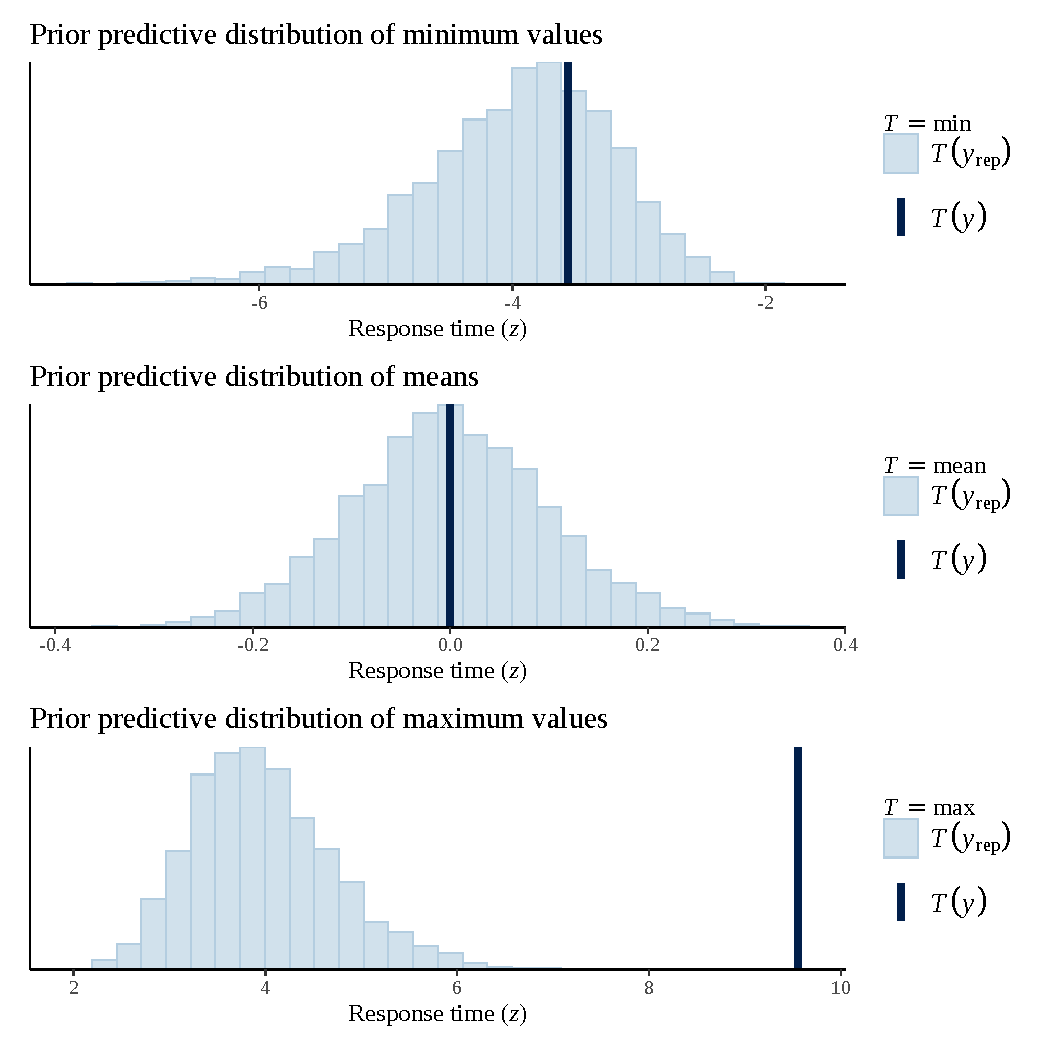
\includegraphics[width=0.8\linewidth]{C:/Users/Pablo/Documents/semanticpriming-semanticdecision-lexicaldecision/semanticpriming/bayesian_analysis/prior_predictive_checks/plots/semanticpriming_priorpredictivecheck_informativepriors} 

}

\caption{Prior predictive checks for the Gaussian, informative prior model from the semantic priming study. \(y\) = observed data; \(y_{rep}\) = predicted data.}\label{fig:semanticpriming-priorpredictivecheck-informativepriors}
\end{figure}



\begin{figure}

{\centering 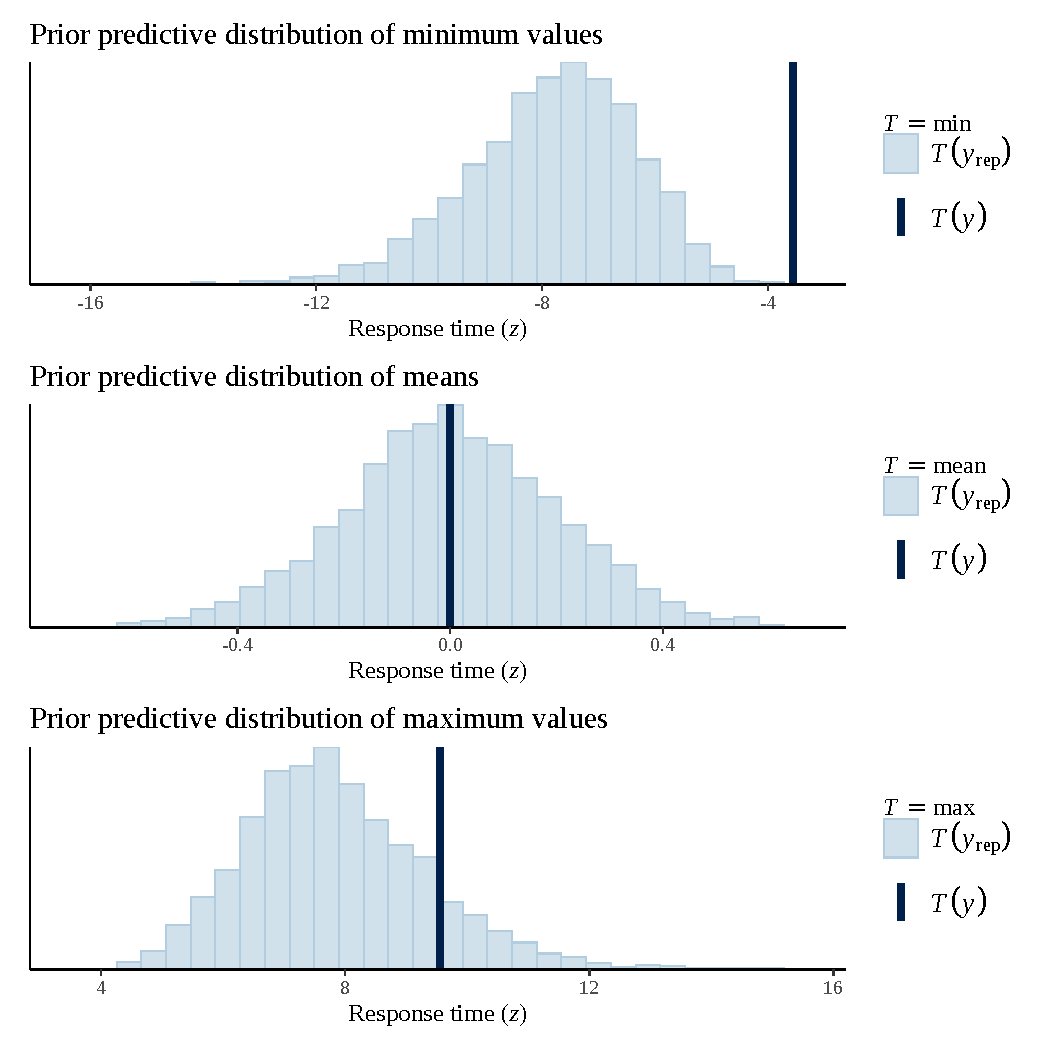
\includegraphics[width=0.8\linewidth]{C:/Users/Pablo/Documents/semanticpriming-semanticdecision-lexicaldecision/semanticpriming/bayesian_analysis/prior_predictive_checks/plots/semanticpriming_priorpredictivecheck_weaklyinformativepriors} 

}

\caption{Prior predictive checks for the Gaussian, weakly-informative prior model from the semantic priming study. \(y\) = observed data; \(y_{rep}\) = predicted data.}\label{fig:semanticpriming-priorpredictivecheck-weaklyinformativepriors}
\end{figure}



\begin{figure}

{\centering 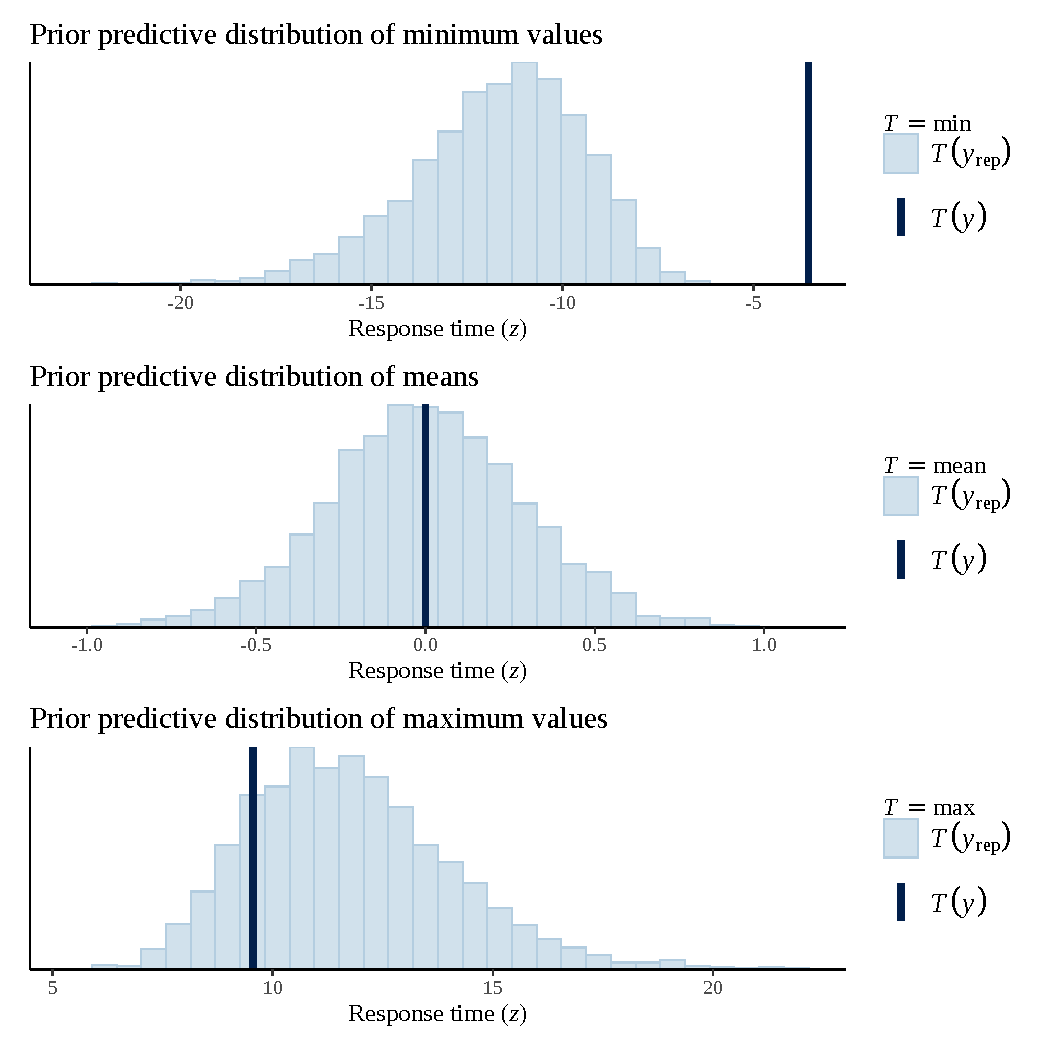
\includegraphics[width=0.8\linewidth]{C:/Users/Pablo/Documents/semanticpriming-semanticdecision-lexicaldecision/semanticpriming/bayesian_analysis/prior_predictive_checks/plots/semanticpriming_priorpredictivecheck_diffusepriors} 

}

\caption{Prior predictive checks for the Gaussian, diffuse prior model from the semantic priming study. \(y\) = observed data; \(y_{rep}\) = predicted data.}\label{fig:semanticpriming-priorpredictivecheck-diffusepriors}
\end{figure}

In contrast to the above results, Figures \ref{fig:semanticpriming-priorpredictivecheck-informativepriors-exgaussian}, \ref{fig:semanticpriming-priorpredictivecheck-weaklyinformativepriors-exgaussian} and \ref{fig:semanticpriming-priorpredictivecheck-diffusepriors-exgaussian} demonstrate that, when an ex-Gaussian distribution was used, the priors fitted the data far better, which converged with the results of a similar comparison performed by Rodríguez-Ferreiro et al. (2020) (see supplementary materials of the latter study).



\begin{figure}

{\centering 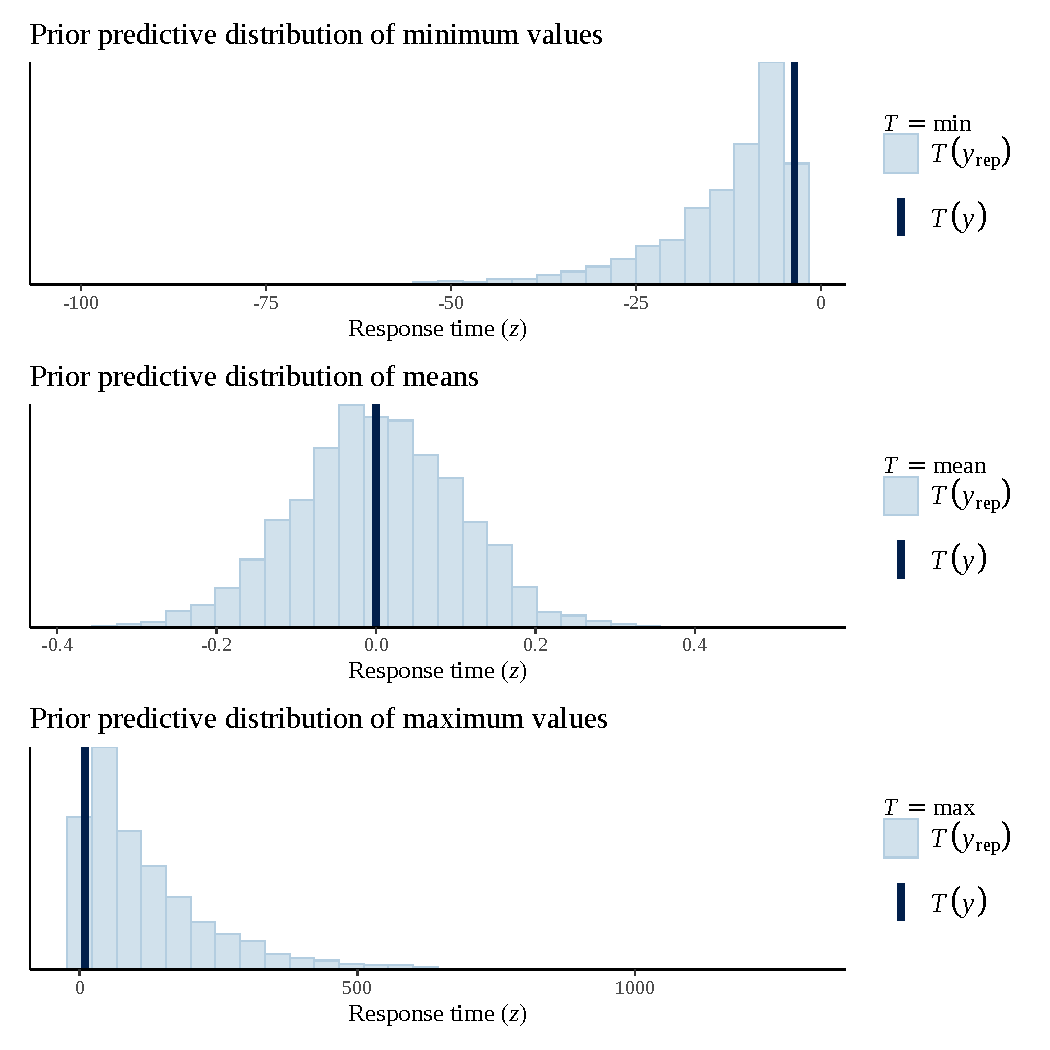
\includegraphics[width=0.8\linewidth]{C:/Users/Pablo/Documents/semanticpriming-semanticdecision-lexicaldecision/semanticpriming/bayesian_analysis/prior_predictive_checks/plots/semanticpriming_priorpredictivecheck_informativepriors_exgaussian} 

}

\caption{Prior predictive checks for the ex-Gaussian, informative prior model from the semantic priming study. \(y\) = observed data; \(y_{rep}\) = predicted data.}\label{fig:semanticpriming-priorpredictivecheck-informativepriors-exgaussian}
\end{figure}



\begin{figure}

{\centering 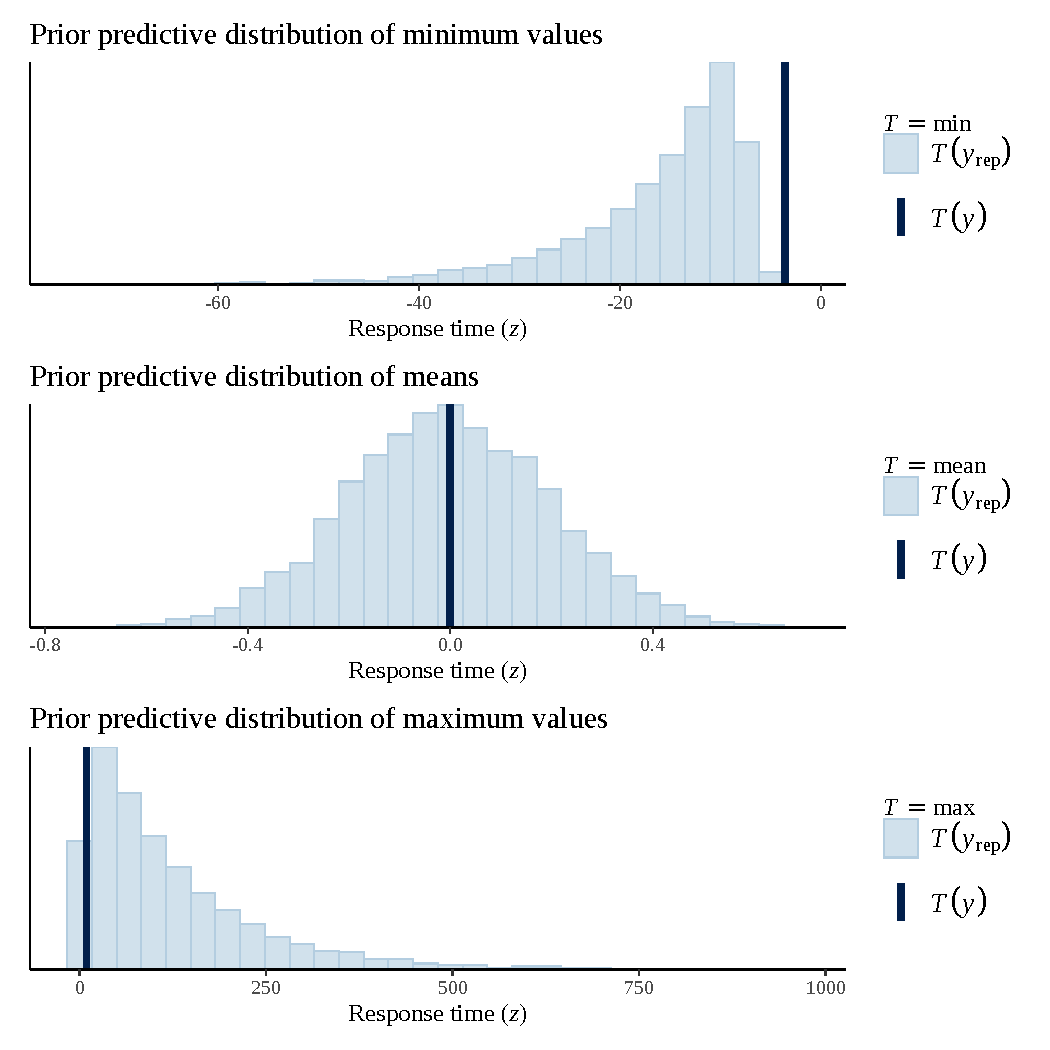
\includegraphics[width=0.8\linewidth]{C:/Users/Pablo/Documents/semanticpriming-semanticdecision-lexicaldecision/semanticpriming/bayesian_analysis/prior_predictive_checks/plots/semanticpriming_priorpredictivecheck_weaklyinformativepriors_exgaussian} 

}

\caption{Prior predictive checks for the ex-Gaussian, weakly-informative prior model from the semantic priming study. \(y\) = observed data; \(y_{rep}\) = predicted data.}\label{fig:semanticpriming-priorpredictivecheck-weaklyinformativepriors-exgaussian}
\end{figure}



\begin{figure}

{\centering 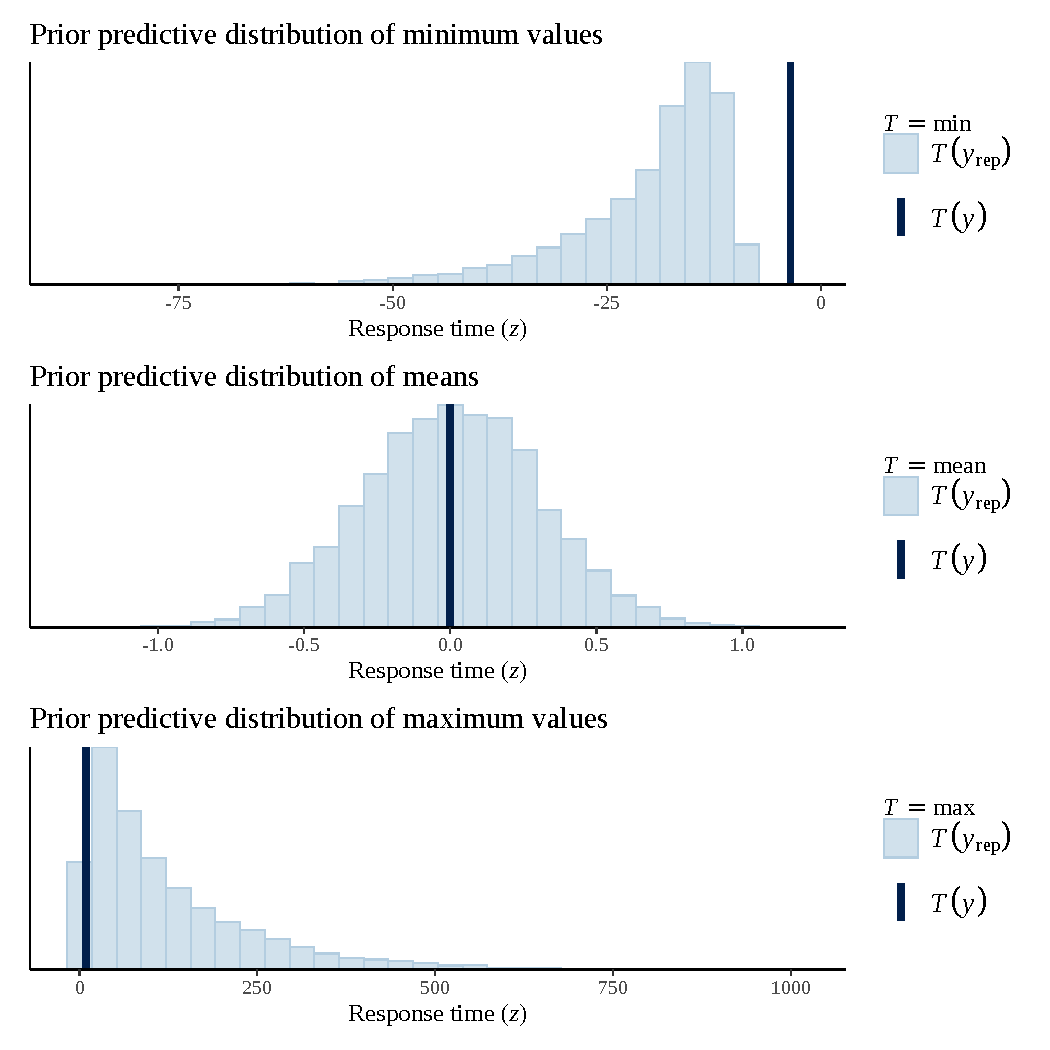
\includegraphics[width=0.8\linewidth]{C:/Users/Pablo/Documents/semanticpriming-semanticdecision-lexicaldecision/semanticpriming/bayesian_analysis/prior_predictive_checks/plots/semanticpriming_priorpredictivecheck_diffusepriors_exgaussian} 

}

\caption{Prior predictive checks for the ex-Gaussian, diffuse prior model from the semantic priming study. \(y\) = observed data; \(y_{rep}\) = predicted data.}\label{fig:semanticpriming-priorpredictivecheck-diffusepriors-exgaussian}
\end{figure}

\hypertarget{posterior-predictive-checks}{%
\subsubsection{Posterior predictive checks}\label{posterior-predictive-checks}}

Based on the above results, the ex-Gaussian distribution was used in the final models. Figure \ref{fig:semanticpriming-posteriorpredictivechecks-allpriors-exgaussian} presents the posterior predictive checks for the latter models. The interpretation of these plots is simple: the distributions of the observed (\(y\)) and the predicted data (\(y_{rep}\)) should be as similar as possible. As such, the plots below suggest that the results are trustworthy.



\begin{figure}

{\centering 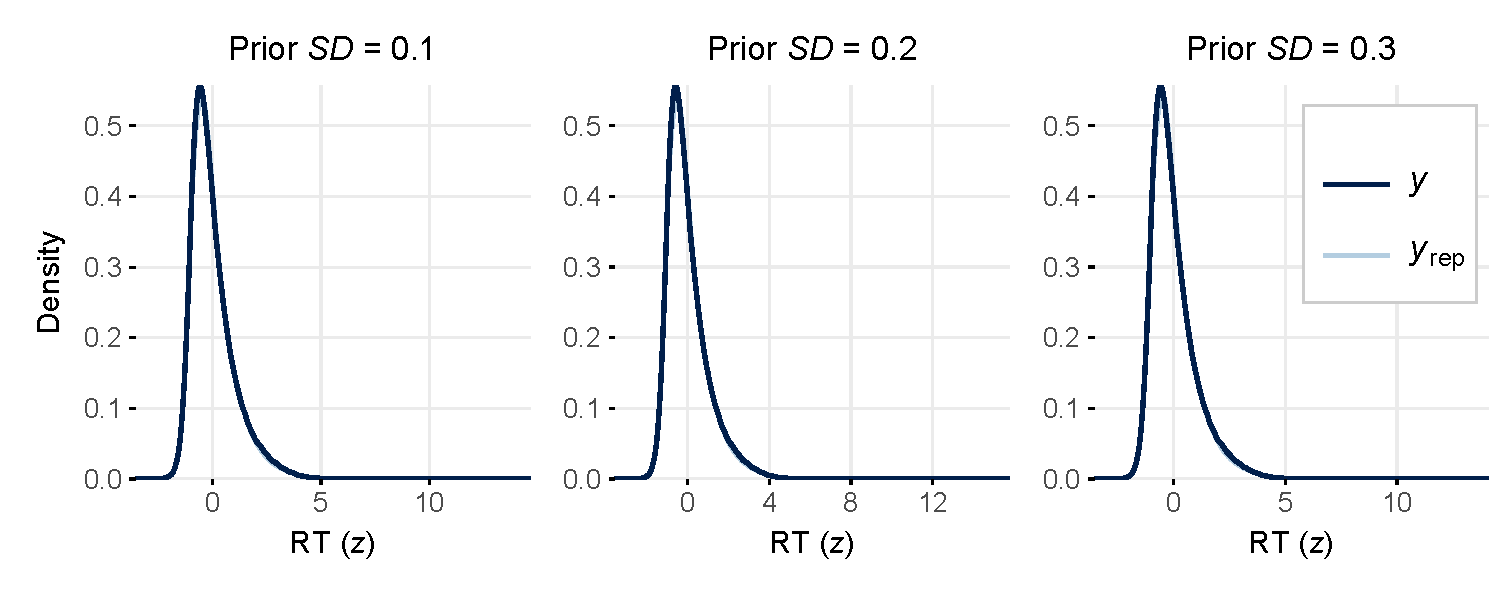
\includegraphics[width=1\linewidth]{C:/Users/Pablo/Documents/semanticpriming-semanticdecision-lexicaldecision/semanticpriming/bayesian_analysis/posterior_predictive_checks/plots/semanticpriming_posteriorpredictivechecks_allpriors_exgaussian} 

}

\caption{Posterior predictive checks for the (ex-Gaussian) models from the semantic priming study. The observed data (\(y\)) and the predicted data (\(y_{rep}\)) almost entirely overlap with each other, demonstrating a very good fit.}\label{fig:semanticpriming-posteriorpredictivechecks-allpriors-exgaussian}
\end{figure}

\hypertarget{study-2-semantic-decision-3}{%
\subsection{Study 2: Semantic decision}\label{study-2-semantic-decision-3}}

\hypertarget{prior-predictive-checks-1}{%
\subsubsection{Prior predictive checks}\label{prior-predictive-checks-1}}

Figures \ref{fig:semanticdecision-priorpredictivecheck-informativepriors}, \ref{fig:semanticdecision-priorpredictivecheck-weaklyinformativepriors} and \ref{fig:semanticdecision-priorpredictivecheck-diffusepriors} show the prior predictive checks for the Gaussian models (for background on these checks, see \protect\hyperlink{study1-bayesian-diagnostics}{\underline{Study 1}}). The three plots---corresponding to models that used the default Gaussian distribution---show that the priors fitted the data acceptably but not very well.



\begin{figure}

{\centering 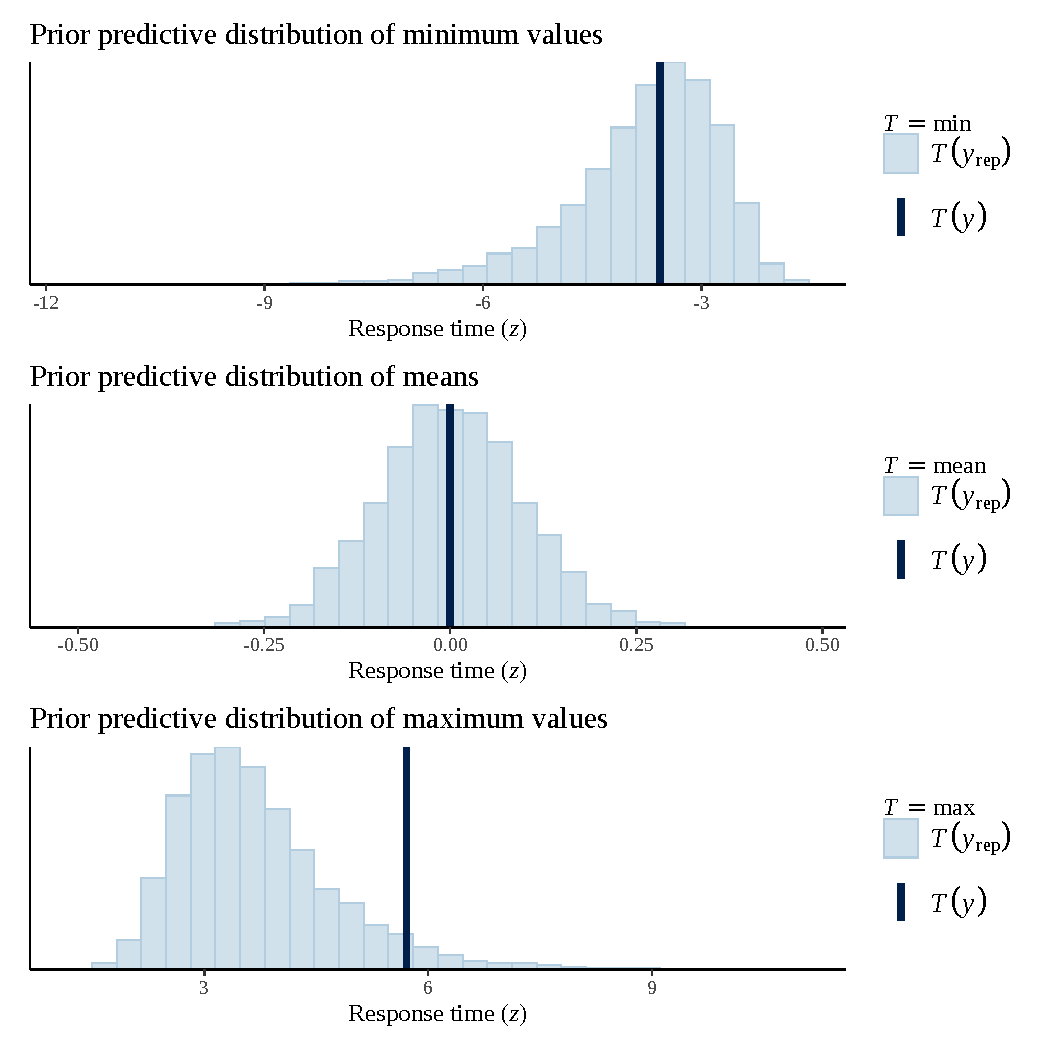
\includegraphics[width=0.8\linewidth]{C:/Users/Pablo/Documents/semanticpriming-semanticdecision-lexicaldecision/semanticdecision/bayesian_analysis/prior_predictive_checks/plots/semanticdecision_priorpredictivecheck_informativepriors} 

}

\caption{Prior predictive checks for the Gaussian, informative prior model from the semantic decision study. \(y\) = observed data; \(y_{rep}\) = predicted data.}\label{fig:semanticdecision-priorpredictivecheck-informativepriors}
\end{figure}



\begin{figure}

{\centering 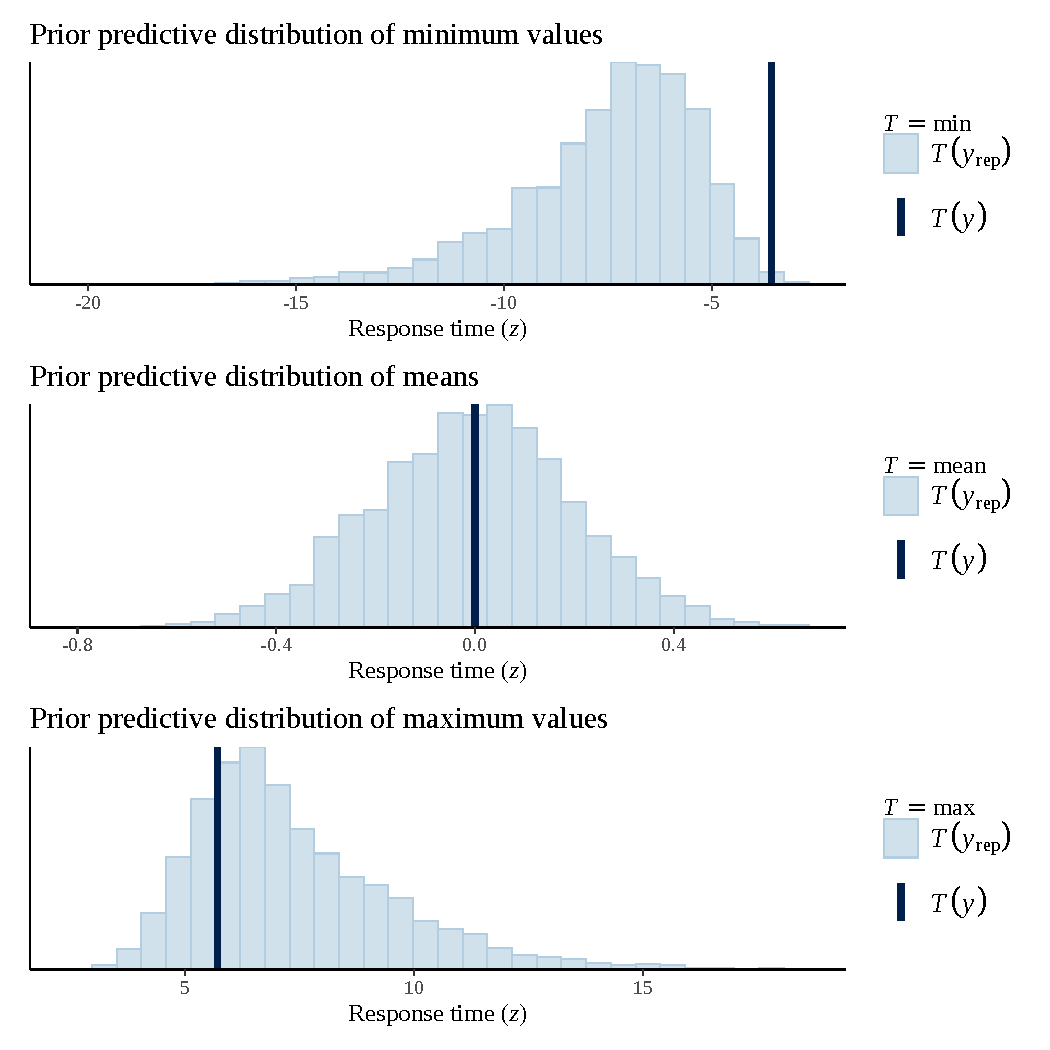
\includegraphics[width=0.8\linewidth]{C:/Users/Pablo/Documents/semanticpriming-semanticdecision-lexicaldecision/semanticdecision/bayesian_analysis/prior_predictive_checks/plots/semanticdecision_priorpredictivecheck_weaklyinformativepriors} 

}

\caption{Prior predictive checks for the Gaussian, weakly-informative prior model from the semantic decision study. \(y\) = observed data; \(y_{rep}\) = predicted data.}\label{fig:semanticdecision-priorpredictivecheck-weaklyinformativepriors}
\end{figure}



\begin{figure}

{\centering 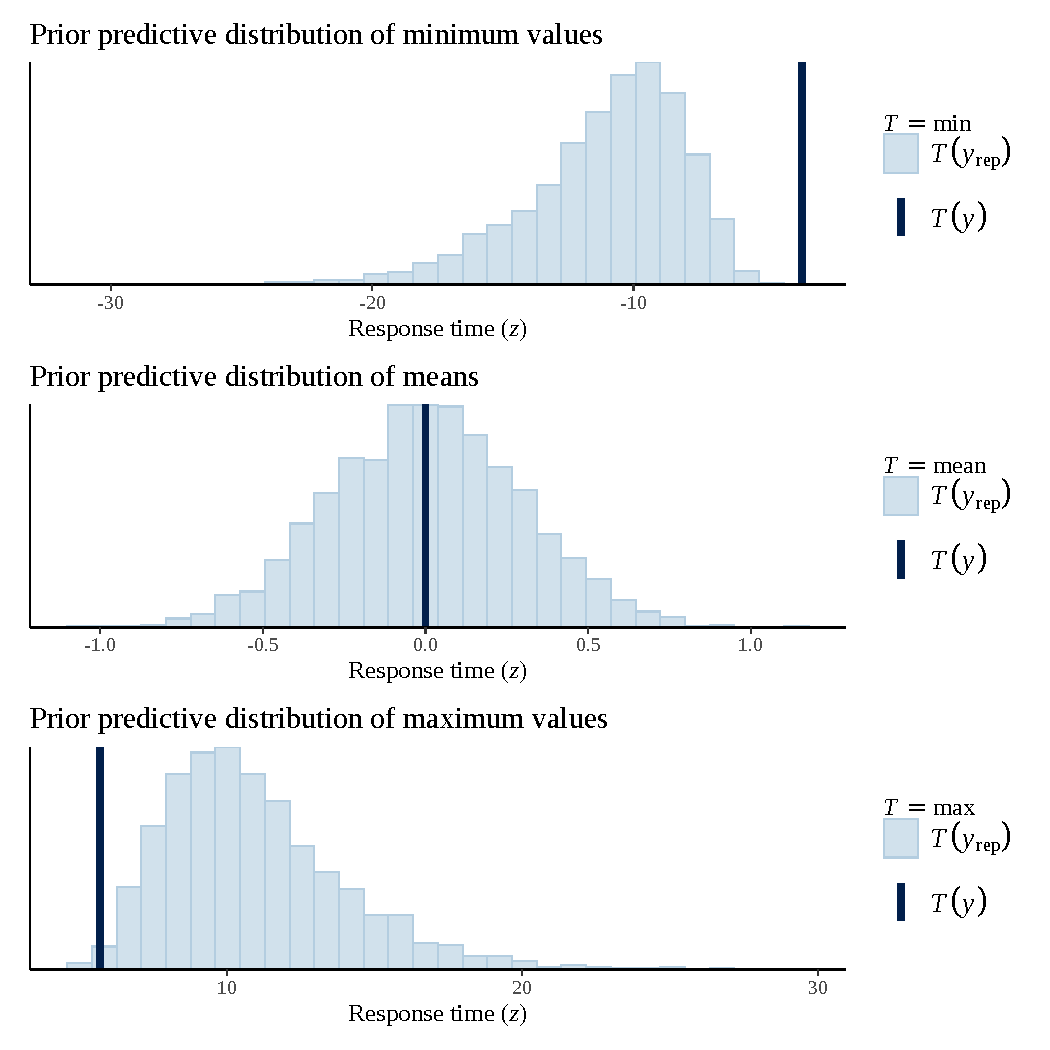
\includegraphics[width=0.8\linewidth]{C:/Users/Pablo/Documents/semanticpriming-semanticdecision-lexicaldecision/semanticdecision/bayesian_analysis/prior_predictive_checks/plots/semanticdecision_priorpredictivecheck_diffusepriors} 

}

\caption{Prior predictive checks for the Gaussian, diffuse prior model from the semantic decision study. \(y\) = observed data; \(y_{rep}\) = predicted data.}\label{fig:semanticdecision-priorpredictivecheck-diffusepriors}
\end{figure}

In contrast to the results from the Gaussian models, Figures \ref{fig:semanticdecision-priorpredictivecheck-informativepriors-exgaussian}, \ref{fig:semanticdecision-priorpredictivecheck-weaklyinformativepriors-exgaussian} and \ref{fig:semanticdecision-priorpredictivecheck-diffusepriors-exgaussian} demonstrate that, when an ex-Gaussian distribution was used, the priors fitted the data far better, which converged with the results found in Study 1.



\begin{figure}

{\centering 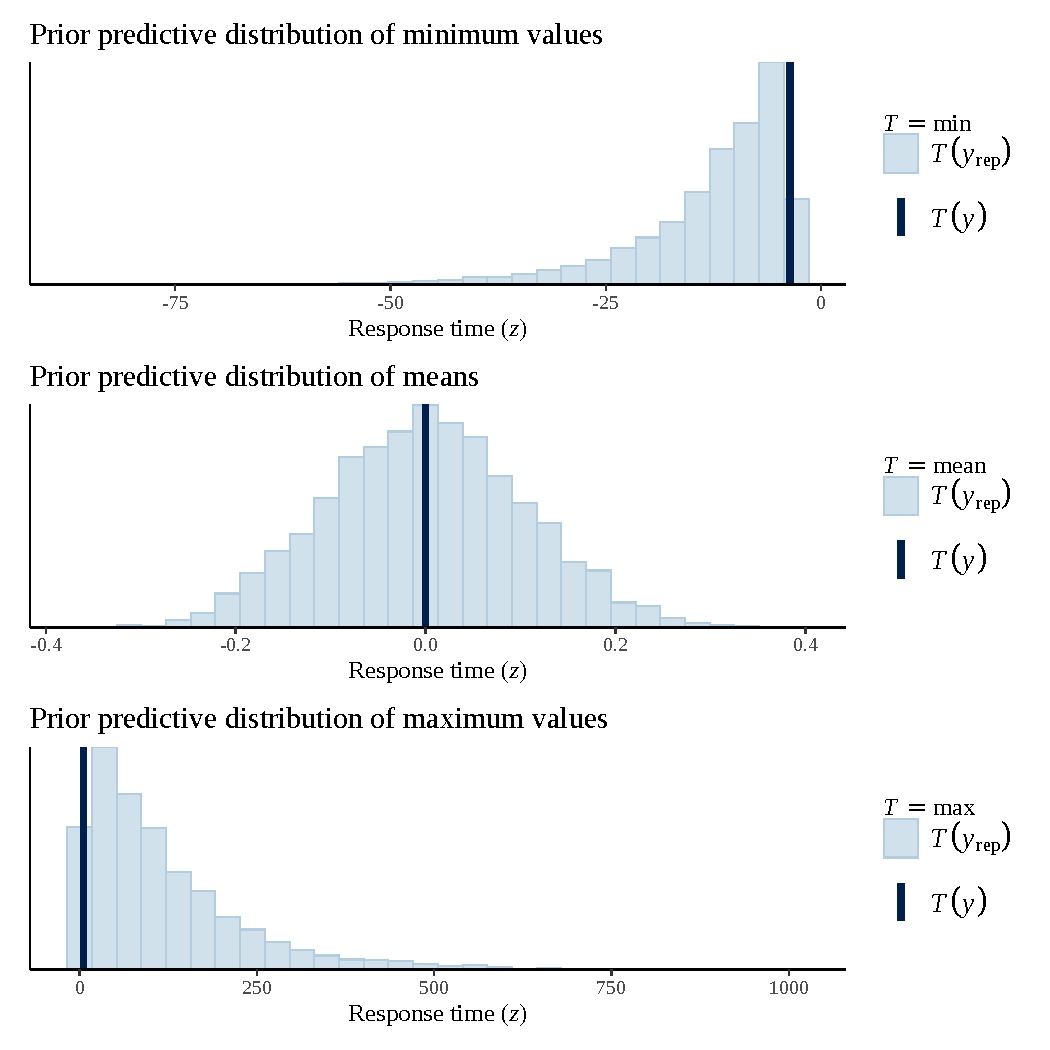
\includegraphics[width=0.8\linewidth]{C:/Users/Pablo/Documents/semanticpriming-semanticdecision-lexicaldecision/semanticdecision/bayesian_analysis/prior_predictive_checks/plots/semanticdecision_priorpredictivecheck_informativepriors_exgaussian} 

}

\caption{Prior predictive checks for the ex-Gaussian, informative prior model from the semantic decision study. \(y\) = observed data; \(y_{rep}\) = predicted data.}\label{fig:semanticdecision-priorpredictivecheck-informativepriors-exgaussian}
\end{figure}



\begin{figure}

{\centering 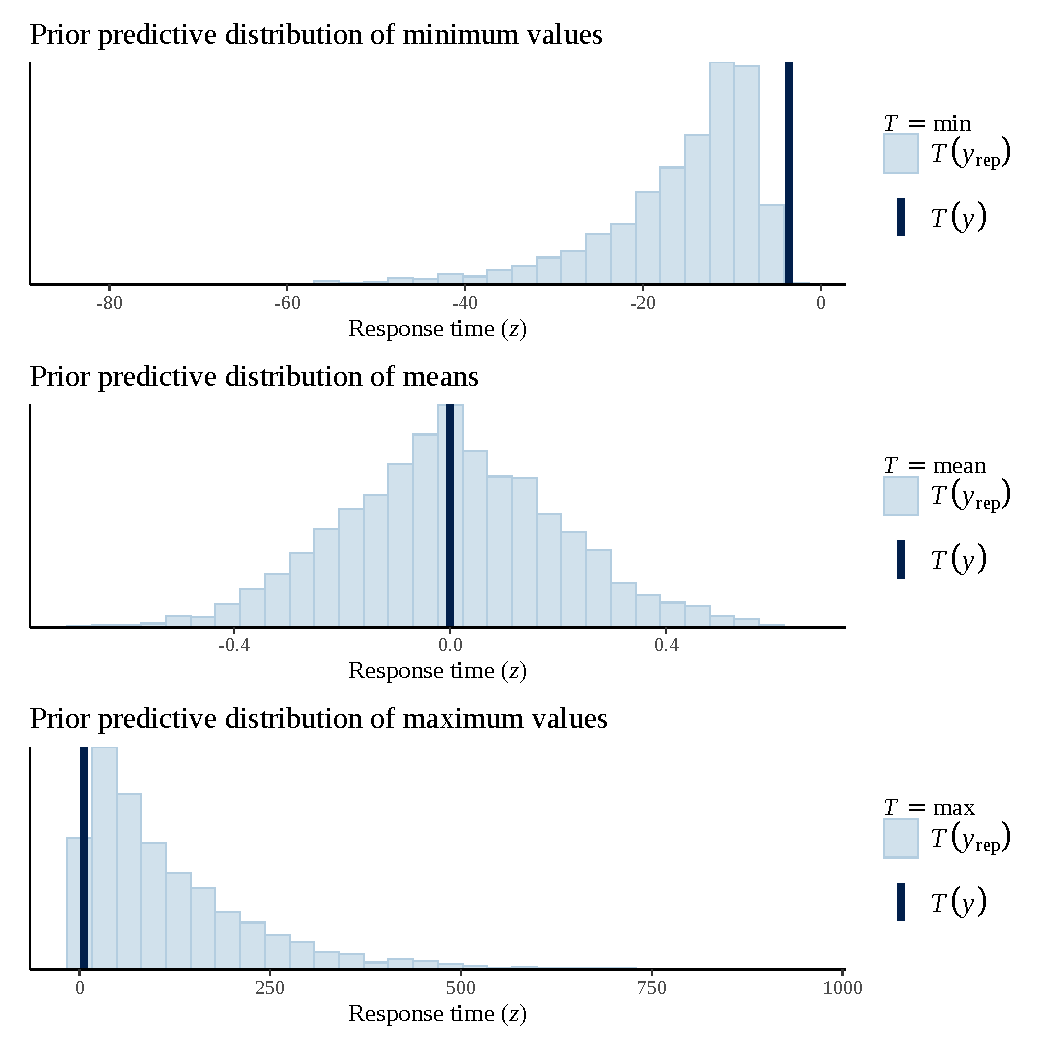
\includegraphics[width=0.8\linewidth]{C:/Users/Pablo/Documents/semanticpriming-semanticdecision-lexicaldecision/semanticdecision/bayesian_analysis/prior_predictive_checks/plots/semanticdecision_priorpredictivecheck_weaklyinformativepriors_exgaussian} 

}

\caption{Prior predictive checks for the ex-Gaussian, weakly-informative prior model from the semantic decision study. \(y\) = observed data; \(y_{rep}\) = predicted data.}\label{fig:semanticdecision-priorpredictivecheck-weaklyinformativepriors-exgaussian}
\end{figure}



\begin{figure}

{\centering \includegraphics[width=0.8\linewidth]{C:/Users/Pablo/Documents/semanticpriming-semanticdecision-lexicaldecision/semanticdecision/bayesian_analysis/prior_predictive_checks/plots/semanticdecision_priorpredictivecheck_diffusepriors_exgaussian} 

}

\caption{Prior predictive checks for the ex-Gaussian, diffuse prior model from the semantic decision study. \(y\) = observed data; \(y_{rep}\) = predicted data.}\label{fig:semanticdecision-priorpredictivecheck-diffusepriors-exgaussian}
\end{figure}

\hypertarget{posterior-predictive-checks-1}{%
\subsubsection{Posterior predictive checks}\label{posterior-predictive-checks-1}}

Based on the above results, the ex-Gaussian distribution was used in the final models. Figure \ref{fig:semanticdecision-posteriorpredictivechecks-allpriors-exgaussian} presents the posterior predictive checks for the latter models. The interpretation of these plots is simple: the distributions of the observed (\(y\)) and the predicted data (\(y_{rep}\)) should be as similar as possible. As such, the plots below suggest that the results are not entirely trustworthy. Indeed, the results themselves (\protect\hyperlink{appendix-E-Bayesian-analysis-results}{\underline{Appendix E}}) are clearly not valid.



\begin{figure}

{\centering \includegraphics[width=1\linewidth]{C:/Users/Pablo/Documents/semanticpriming-semanticdecision-lexicaldecision/semanticdecision/bayesian_analysis/posterior_predictive_checks/plots/semanticdecision_posteriorpredictivechecks_allpriors_exgaussian} 

}

\caption{Posterior predictive checks for the (ex-Gaussian) models from the semantic decision study. \(y\) = observed data; \(y_{rep}\) = predicted data.}\label{fig:semanticdecision-posteriorpredictivechecks-allpriors-exgaussian}
\end{figure}

\hypertarget{study-3-lexical-decision-2}{%
\subsection{Study 3: Lexical decision}\label{study-3-lexical-decision-2}}

\hypertarget{prior-predictive-checks-2}{%
\subsubsection{Prior predictive checks}\label{prior-predictive-checks-2}}

Figures \ref{fig:lexicaldecision-priorpredictivecheck-informativepriors}, \ref{fig:lexicaldecision-priorpredictivecheck-weaklyinformativepriors} and \ref{fig:lexicaldecision-priorpredictivecheck-diffusepriors} show the prior predictive checks for the Gaussian models (for background on these checks, see \protect\hyperlink{study1-bayesian-diagnostics}{\underline{Study 1}}). The three plots---corresponding to models that used the default Gaussian distribution---show that the priors fitted the data acceptably but not very well.



\begin{figure}

{\centering \includegraphics[width=0.8\linewidth]{C:/Users/Pablo/Documents/semanticpriming-semanticdecision-lexicaldecision/lexicaldecision/bayesian_analysis/prior_predictive_checks/plots/lexicaldecision_priorpredictivecheck_informativepriors} 

}

\caption{Prior predictive checks for the Gaussian, informative prior model from the lexical decision study. \(y\) = observed data; \(y_{rep}\) = predicted data.}\label{fig:lexicaldecision-priorpredictivecheck-informativepriors}
\end{figure}



\begin{figure}

{\centering \includegraphics[width=0.8\linewidth]{C:/Users/Pablo/Documents/semanticpriming-semanticdecision-lexicaldecision/lexicaldecision/bayesian_analysis/prior_predictive_checks/plots/lexicaldecision_priorpredictivecheck_weaklyinformativepriors} 

}

\caption{Prior predictive checks for the Gaussian, weakly-informative prior model from the lexical decision study. \(y\) = observed data; \(y_{rep}\) = predicted data.}\label{fig:lexicaldecision-priorpredictivecheck-weaklyinformativepriors}
\end{figure}



\begin{figure}

{\centering \includegraphics[width=0.8\linewidth]{C:/Users/Pablo/Documents/semanticpriming-semanticdecision-lexicaldecision/lexicaldecision/bayesian_analysis/prior_predictive_checks/plots/lexicaldecision_priorpredictivecheck_diffusepriors} 

}

\caption{Prior predictive checks for the Gaussian, diffuse prior model from the lexical decision study. \(y\) = observed data; \(y_{rep}\) = predicted data.}\label{fig:lexicaldecision-priorpredictivecheck-diffusepriors}
\end{figure}

In contrast to the results from the Gaussian models, Figures \ref{fig:lexicaldecision-priorpredictivecheck-informativepriors-exgaussian}, \ref{fig:lexicaldecision-priorpredictivecheck-weaklyinformativepriors-exgaussian} and \ref{fig:lexicaldecision-priorpredictivecheck-diffusepriors-exgaussian} demonstrate that, when an ex-Gaussian distribution was used, the priors fitted the data far better, which converged with the results found in Studies 1 and 2.



\begin{figure}

{\centering \includegraphics[width=0.8\linewidth]{C:/Users/Pablo/Documents/semanticpriming-semanticdecision-lexicaldecision/lexicaldecision/bayesian_analysis/prior_predictive_checks/plots/lexicaldecision_priorpredictivecheck_informativepriors_exgaussian} 

}

\caption{Prior predictive checks for the ex-Gaussian, informative prior model from the lexical decision study. \(y\) = observed data; \(y_{rep}\) = predicted data.}\label{fig:lexicaldecision-priorpredictivecheck-informativepriors-exgaussian}
\end{figure}



\begin{figure}

{\centering \includegraphics[width=0.8\linewidth]{C:/Users/Pablo/Documents/semanticpriming-semanticdecision-lexicaldecision/lexicaldecision/bayesian_analysis/prior_predictive_checks/plots/lexicaldecision_priorpredictivecheck_weaklyinformativepriors_exgaussian} 

}

\caption{Prior predictive checks for the ex-Gaussian, weakly-informative prior model from the lexical decision study. \(y\) = observed data; \(y_{rep}\) = predicted data.}\label{fig:lexicaldecision-priorpredictivecheck-weaklyinformativepriors-exgaussian}
\end{figure}



\begin{figure}

{\centering \includegraphics[width=0.8\linewidth]{C:/Users/Pablo/Documents/semanticpriming-semanticdecision-lexicaldecision/lexicaldecision/bayesian_analysis/prior_predictive_checks/plots/lexicaldecision_priorpredictivecheck_diffusepriors_exgaussian} 

}

\caption{Prior predictive checks for the ex-Gaussian, diffuse prior model from the lexical decision study. \(y\) = observed data; \(y_{rep}\) = predicted data.}\label{fig:lexicaldecision-priorpredictivecheck-diffusepriors-exgaussian}
\end{figure}

\hypertarget{posterior-predictive-checks-2}{%
\subsubsection{Posterior predictive checks}\label{posterior-predictive-checks-2}}

Based on the above results, the ex-Gaussian distribution was used in the final models. Figure \ref{fig:lexicaldecision-posteriorpredictivechecks-allpriors-exgaussian} presents the posterior predictive checks for the latter models. The interpretation of these plots is simple: the distributions of the observed (\(y\)) and the predicted data (\(y_{rep}\)) should be as similar as possible. As such, the plots below suggest that the results are trustworthy.



\begin{figure}

{\centering \includegraphics[width=1\linewidth]{C:/Users/Pablo/Documents/semanticpriming-semanticdecision-lexicaldecision/lexicaldecision/bayesian_analysis/posterior_predictive_checks/plots/lexicaldecision_posteriorpredictivechecks_allpriors_exgaussian} 

}

\caption{Posterior predictive checks for the (ex-Gaussian) models from the lexical decision study. \(y\) = observed data; \(y_{rep}\) = predicted data.}\label{fig:lexicaldecision-posteriorpredictivechecks-allpriors-exgaussian}
\end{figure}

\clearpage

\renewcommand{\thefigure}{D\arabic{figure}} \setcounter{figure}{0}
\renewcommand{\thetable}{D\arabic{table}} \setcounter{table}{0}

\hypertarget{appendix-D-interaction-plots}{%
\section{Appendix D: Further interaction plots}\label{appendix-D-interaction-plots}}

Figures \ref{fig:semanticpriming-interactions-with-attentional-control} -- \ref{fig:lexicaldecision-interaction-word-concreteness-gender} present interactions that were not displayed in the main article. All interaction plots are based on the frequentist analysis.

\hypertarget{study-1-semantic-priming-3}{%
\subsection{Study 1: Semantic priming}\label{study-1-semantic-priming-3}}



\begin{figure}

{\centering \includegraphics[width=0.85\linewidth]{C:/Users/Pablo/Documents/semanticpriming-semanticdecision-lexicaldecision/semanticpriming/frequentist_analysis/plots/semanticpriming-interactions-with-attentional-control} 

}

\caption{Interactions of attentional control with language-based similarity (panel a) and with visual-strength difference (panel b). Attentional control is constrained to deciles (10 sections) in this plot, whereas in the statistical analysis it contained more values within the current range. \(n\) = number of participants contained between deciles.}\label{fig:semanticpriming-interactions-with-attentional-control}
\end{figure}

\begin{figure}

{\centering \includegraphics[width=0.7\linewidth]{C:/Users/Pablo/Documents/semanticpriming-semanticdecision-lexicaldecision/semanticpriming/frequentist_analysis/plots/semanticpriming-interaction-word-concreteness-difference-SOA} 

}

\caption{Interaction between stimulus onset asynchrony (SOA) and word-concreteness difference. SOA was analysed using $z$-scores, but for clarity, the basic labels are used in the legend.}\label{fig:semanticpriming-interaction-word-concreteness-difference-SOA}
\end{figure}



\begin{figure}

{\centering \includegraphics[width=0.9\linewidth]{C:/Users/Pablo/Documents/semanticpriming-semanticdecision-lexicaldecision/semanticpriming/frequentist_analysis/plots/semanticpriming-interaction-word-concreteness-difference-vocabulary-size} 

}

\caption{Interaction between word-concreteness difference and vocabulary size. Vocabulary size is constrained to deciles in this plot, whereas in the statistical analysis it contained more values within the current range. \(n\) = number of participants contained between deciles.}\label{fig:semanticpriming-interaction-word-concreteness-difference-vocabulary-size}
\end{figure}



\begin{figure}

{\centering \includegraphics[width=0.7\linewidth]{C:/Users/Pablo/Documents/semanticpriming-semanticdecision-lexicaldecision/semanticpriming/frequentist_analysis/plots/semanticpriming-interaction-word-concreteness-difference-gender} 

}

\caption{Interaction between word-concreteness difference and gender. Gender was analysed using \(z\)-scores, but for clarity, the basic labels are used in the legend. \(n\) = number of participants contained between deciles.}\label{fig:semanticpriming-interaction-word-concreteness-difference-gender}
\end{figure}

\clearpage

\hypertarget{study-2-semantic-decision-4}{%
\subsection{Study 2: Semantic decision}\label{study-2-semantic-decision-4}}



\begin{figure}

{\centering \includegraphics[width=0.95\linewidth]{C:/Users/Pablo/Documents/semanticpriming-semanticdecision-lexicaldecision/semanticdecision/frequentist_analysis/plots/semanticdecision-interactions-with-information-uptake} 

}

\caption{Interactions of information uptake with word co-occurrence (panel a) and with visual strength (panel b). Information uptake is constrained to deciles in this plot, whereas in the statistical analysis it contained more values within the current range. \(n\) = number of participants contained between deciles.}\label{fig:semanticdecision-interactions-with-information-uptake}
\end{figure}

\clearpage

\hypertarget{study-3-lexical-decision-3}{%
\subsection{Study 3: Lexical decision}\label{study-3-lexical-decision-3}}



\begin{figure}

{\centering \includegraphics[width=0.9\linewidth]{C:/Users/Pablo/Documents/semanticpriming-semanticdecision-lexicaldecision/lexicaldecision/frequentist_analysis/plots/lexicaldecision-interaction-word-concreteness-vocabulary-age} 

}

\caption{Interaction between word concreteness and vocabulary age. Vocabulary age is constrained to sextiles (6 sections) in this plot, whereas in the statistical analysis it contained more values within the current range. \(n\) = number of participants contained between sextiles.}\label{fig:lexicaldecision-interaction-word-concreteness-vocabulary-age}
\end{figure}



\begin{figure}

{\centering \includegraphics[width=0.65\linewidth]{C:/Users/Pablo/Documents/semanticpriming-semanticdecision-lexicaldecision/lexicaldecision/frequentist_analysis/plots/lexicaldecision-interaction-word-concreteness-gender} 

}

\caption{Interaction between word concreteness and gender. Gender was analysed using \(z\)-scores, but for clarity, the basic labels are used in the legend. \(n\) = number of participants contained between sextiles.}\label{fig:lexicaldecision-interaction-word-concreteness-gender}
\end{figure}

\clearpage

\renewcommand{\thefigure}{E\arabic{figure}} \setcounter{figure}{0}
\renewcommand{\thetable}{E\arabic{table}} \setcounter{table}{0}

\hypertarget{appendix-E-Bayesian-analysis-results}{%
\section{Appendix E: Results from the Bayesian analyses}\label{appendix-E-Bayesian-analysis-results}}

This appendix presents extended results from the Bayesian analyses, containing a prior sensitivity analysis (Schoot et al., 2021). For each study, three tables are presented that contain the results from the informative prior model (\(SD\) = 0.1), the weakly-informative prior model (\(SD\) = 0.2) and the diffuse prior model (\(SD\) = 0.3). All models had an exponentially modified Gaussian (dubbed `ex-Gaussian') distribution with an identity link function (for background, see main text and \protect\hyperlink{appendix-C-Bayesian-analysis-diagnostics}{\underline{Appendix C}}). The \(\widehat R\) value is a convergence diagnostic that should ideally be smaller than 1.01 (Vehtari et al., 2021).

The approach used in this Bayesian analysis is that of estimation (Tendeiro \& Kiers, 2019; also see Schmalz et al., 2021). Thus, the estimates were interpreted by considering the position of their credible intervals in relation to the predicted value of RT (\(z\)). That is, the closer an interval is to a value of 0 on the predicted RT (\(z\)), the smaller the effect of that predictor. For instance, an interval that is symmetrically centred on 0 indicates a very small effect, whereas---in comparison---an interval that does not include 0 indicates a far larger effect (for other examples of this approach, see Milek et al., 2018; Pregla et al., 2021; Rodríguez-Ferreiro et al., 2020).

\hypertarget{study-1-semantic-priming-4}{%
\subsection{Study 1: Semantic priming}\label{study-1-semantic-priming-4}}

Table \ref{tab:semanticpriming-informativepriors-model} presents the results of the informative prior model, Table \ref{tab:semanticpriming-weaklyinformativepriors-model} those of the weakly-informative prior model, and Table \ref{tab:semanticpriming-diffusepriors-model} those of the diffuse prior model.

\begin{table}[!h]

\caption{\label{tab:semanticpriming-informativepriors-model}Informative prior model for the semantic priming study.}
\centering
\begin{threeparttable}
\begin{tabular}[t]{lrrrr}
\toprule
\multicolumn{1}{c}{ } & \multicolumn{1}{c}{$\upbeta$} & \multicolumn{1}{c}{$SE$} & \multicolumn{1}{c}{95\% CrI} & \multicolumn{1}{c}{$\widehat R$}\\
\midrule
(Intercept) & 0.00 & 0.00 & {}[0.00, 0.01] & 1.00\\
\addlinespace[0.3em]
\multicolumn{5}{l}{\textbf{Individual differences}}\\
\cellcolor{gray!6}{\hspace{1em}Attentional control} & \cellcolor{gray!6}{0.00} & \cellcolor{gray!6}{0.00} & \cellcolor{gray!6}{{}[0.00, 0.01]} & \cellcolor{gray!6}{1.00}\\
\hspace{1em}Vocabulary size $^{\text{a}}$ & -0.01 & 0.00 & {}[-0.01, 0.00] & 1.00\\
\hspace{1em}Gender $^{\text{a}}$ & 0.00 & 0.00 & {}[0.00, 0.01] & 1.00\\
\addlinespace[0.3em]
\multicolumn{5}{l}{\textbf{Target-word lexical covariates}}\\
\cellcolor{gray!6}{\hspace{1em}Word frequency} & \cellcolor{gray!6}{-0.11} & \cellcolor{gray!6}{0.00} & \cellcolor{gray!6}{{}[-0.12, -0.11]} & \cellcolor{gray!6}{1.00}\\
\cellcolor{gray!6}{\hspace{1em}Number of syllables} & \cellcolor{gray!6}{0.07} & \cellcolor{gray!6}{0.00} & \cellcolor{gray!6}{{}[0.06, 0.07]} & \cellcolor{gray!6}{1.00}\\
\addlinespace[0.3em]
\multicolumn{5}{l}{\textbf{Prime--target relationship}}\\
\cellcolor{gray!6}{\hspace{1em}Word-concreteness difference} & \cellcolor{gray!6}{0.01} & \cellcolor{gray!6}{0.00} & \cellcolor{gray!6}{{}[0.00, 0.01]} & \cellcolor{gray!6}{1.00}\\
\hspace{1em}Language-based similarity $^{\text{b}}$ & -0.06 & 0.00 & {}[-0.07, -0.06] & 1.00\\
\hspace{1em}Visual-strength difference $^{\text{b}}$ & 0.01 & 0.00 & {}[0.01, 0.02] & 1.00\\
\addlinespace[0.3em]
\multicolumn{5}{l}{\textbf{Task condition}}\\
\hspace{1em}Stimulus onset asynchrony (SOA) $^{\text{b}}$ & 0.03 & 0.01 & {}[0.02, 0.04] & 1.00\\
\addlinespace[0.3em]
\multicolumn{5}{l}{\textbf{Interactions}}\\
\cellcolor{gray!6}{\hspace{1em}\makecell[l]{Word-concreteness difference  $\times$ \\ \hspace{0.3cm} Vocabulary size}} & \cellcolor{gray!6}{0.00} & \cellcolor{gray!6}{0.00} & \cellcolor{gray!6}{{}[0.00, 0.00]} & \cellcolor{gray!6}{1.00}\\
\cellcolor{gray!6}{\hspace{1em}Word-concreteness difference  $\times$  SOA} & \cellcolor{gray!6}{0.00} & \cellcolor{gray!6}{0.00} & \cellcolor{gray!6}{{}[0.00, 0.00]} & \cellcolor{gray!6}{1.00}\\
\cellcolor{gray!6}{\hspace{1em}Word-concreteness difference  $\times$  Gender} & \cellcolor{gray!6}{0.00} & \cellcolor{gray!6}{0.00} & \cellcolor{gray!6}{{}[0.00, 0.00]} & \cellcolor{gray!6}{1.00}\\
\cellcolor{gray!6}{\hspace{1em}\makecell[l]{Language-based similarity  $\times$ \\ \hspace{0.3cm} Attentional control}} & \cellcolor{gray!6}{0.00} & \cellcolor{gray!6}{0.00} & \cellcolor{gray!6}{{}[-0.01, 0.00]} & \cellcolor{gray!6}{1.00}\\
\cellcolor{gray!6}{\hspace{1em}\makecell[l]{Visual-strength difference  $\times$ \\ \hspace{0.3cm} Attentional control}} & \cellcolor{gray!6}{0.00} & \cellcolor{gray!6}{0.00} & \cellcolor{gray!6}{{}[0.00, 0.00]} & \cellcolor{gray!6}{1.00}\\
\hspace{1em}\makecell[l]{Language-based similarity  $\times$ \\ \hspace{0.3cm} Vocabulary size} & 0.00 & 0.00 & {}[-0.01, 0.00] & 1.00\\
\hspace{1em}\makecell[l]{Visual-strength difference  $\times$ \\ \hspace{0.3cm} Vocabulary size} & 0.00 & 0.00 & {}[0.00, 0.00] & 1.00\\
\hspace{1em}Language-based similarity  $\times$  Gender & 0.00 & 0.00 & {}[-0.01, 0.00] & 1.00\\
\hspace{1em}Visual-strength difference  $\times$  Gender & 0.00 & 0.00 & {}[0.00, 0.00] & 1.00\\
\hspace{1em}Language-based similarity  $\times$  SOA $^{\text{b}}$ & 0.00 & 0.00 & {}[0.00, 0.00] & 1.00\\
\hspace{1em}Visual-strength difference  $\times$  SOA $^{\text{b}}$ & 0.00 & 0.00 & {}[0.00, 0.00] & 1.00\\
\bottomrule
\end{tabular}
\begin{tablenotes}
\item \textit{\linebreak} 
\item \textit{Note}. $\upbeta$ = Estimate based on $z$-scored predictors; \textit{SE} = standard error; \linebreak \phantom{.}CrI = credible interval. Shaded rows contain covariates. Some interactions \linebreak \phantom{.}are split over two lines, with the second line indented. \linebreak \linebreak \phantom{.}$^{\text{a}}$ By-word random slopes were included for this effect. \linebreak \phantom{.}$^{\text{b}}$ By-participant random slopes were included for this effect.
\end{tablenotes}
\end{threeparttable}
\end{table}

\begin{table}[!h]

\caption{\label{tab:semanticpriming-weaklyinformativepriors-model}Weakly-informative prior model for the semantic priming study.}
\centering
\begin{threeparttable}
\begin{tabular}[t]{lrrrr}
\toprule
\multicolumn{1}{c}{ } & \multicolumn{1}{c}{$\upbeta$} & \multicolumn{1}{c}{$SE$} & \multicolumn{1}{c}{95\% CrI} & \multicolumn{1}{c}{$\widehat R$}\\
\midrule
(Intercept) & 0.00 & 0.00 & {}[0.00, 0.01] & 1.00\\
\addlinespace[0.3em]
\multicolumn{5}{l}{\textbf{Individual differences}}\\
\cellcolor{gray!6}{\hspace{1em}Attentional control} & \cellcolor{gray!6}{0.00} & \cellcolor{gray!6}{0.00} & \cellcolor{gray!6}{{}[0.00, 0.01]} & \cellcolor{gray!6}{1.00}\\
\hspace{1em}Vocabulary size $^{\text{a}}$ & -0.01 & 0.00 & {}[-0.01, 0.00] & 1.00\\
\hspace{1em}Gender $^{\text{a}}$ & 0.00 & 0.00 & {}[0.00, 0.01] & 1.00\\
\addlinespace[0.3em]
\multicolumn{5}{l}{\textbf{Target-word lexical covariates}}\\
\cellcolor{gray!6}{\hspace{1em}Word frequency} & \cellcolor{gray!6}{-0.11} & \cellcolor{gray!6}{0.00} & \cellcolor{gray!6}{{}[-0.12, -0.11]} & \cellcolor{gray!6}{1.00}\\
\cellcolor{gray!6}{\hspace{1em}Number of syllables} & \cellcolor{gray!6}{0.07} & \cellcolor{gray!6}{0.00} & \cellcolor{gray!6}{{}[0.06, 0.07]} & \cellcolor{gray!6}{1.00}\\
\addlinespace[0.3em]
\multicolumn{5}{l}{\textbf{Prime--target relationship}}\\
\cellcolor{gray!6}{\hspace{1em}Word-concreteness difference} & \cellcolor{gray!6}{0.01} & \cellcolor{gray!6}{0.00} & \cellcolor{gray!6}{{}[0.00, 0.01]} & \cellcolor{gray!6}{1.00}\\
\hspace{1em}Language-based similarity $^{\text{b}}$ & -0.06 & 0.00 & {}[-0.07, -0.06] & 1.00\\
\hspace{1em}Visual-strength difference $^{\text{b}}$ & 0.01 & 0.00 & {}[0.01, 0.01] & 1.00\\
\addlinespace[0.3em]
\multicolumn{5}{l}{\textbf{Task condition}}\\
\hspace{1em}Stimulus onset asynchrony (SOA) $^{\text{b}}$ & 0.03 & 0.01 & {}[0.02, 0.04] & 1.00\\
\addlinespace[0.3em]
\multicolumn{5}{l}{\textbf{Interactions}}\\
\cellcolor{gray!6}{\hspace{1em}\makecell[l]{Word-concreteness difference  $\times$ \\ \hspace{0.3cm} Vocabulary size}} & \cellcolor{gray!6}{0.00} & \cellcolor{gray!6}{0.00} & \cellcolor{gray!6}{{}[0.00, 0.00]} & \cellcolor{gray!6}{1.00}\\
\cellcolor{gray!6}{\hspace{1em}Word-concreteness difference  $\times$  SOA} & \cellcolor{gray!6}{0.00} & \cellcolor{gray!6}{0.00} & \cellcolor{gray!6}{{}[0.00, 0.00]} & \cellcolor{gray!6}{1.00}\\
\cellcolor{gray!6}{\hspace{1em}Word-concreteness difference  $\times$  Gender} & \cellcolor{gray!6}{0.00} & \cellcolor{gray!6}{0.00} & \cellcolor{gray!6}{{}[0.00, 0.00]} & \cellcolor{gray!6}{1.00}\\
\cellcolor{gray!6}{\hspace{1em}\makecell[l]{Language-based similarity  $\times$ \\ \hspace{0.3cm} Attentional control}} & \cellcolor{gray!6}{0.00} & \cellcolor{gray!6}{0.00} & \cellcolor{gray!6}{{}[-0.01, 0.00]} & \cellcolor{gray!6}{1.00}\\
\cellcolor{gray!6}{\hspace{1em}\makecell[l]{Visual-strength difference  $\times$ \\ \hspace{0.3cm} Attentional control}} & \cellcolor{gray!6}{0.00} & \cellcolor{gray!6}{0.00} & \cellcolor{gray!6}{{}[0.00, 0.00]} & \cellcolor{gray!6}{1.00}\\
\hspace{1em}\makecell[l]{Language-based similarity  $\times$ \\ \hspace{0.3cm} Vocabulary size} & 0.00 & 0.00 & {}[-0.01, 0.00] & 1.00\\
\hspace{1em}\makecell[l]{Visual-strength difference  $\times$ \\ \hspace{0.3cm} Vocabulary size} & 0.00 & 0.00 & {}[0.00, 0.00] & 1.00\\
\hspace{1em}Language-based similarity  $\times$  Gender & 0.00 & 0.00 & {}[-0.01, 0.00] & 1.00\\
\hspace{1em}Visual-strength difference  $\times$  Gender & 0.00 & 0.00 & {}[0.00, 0.00] & 1.00\\
\hspace{1em}Language-based similarity  $\times$  SOA $^{\text{b}}$ & 0.00 & 0.00 & {}[0.00, 0.00] & 1.00\\
\hspace{1em}Visual-strength difference  $\times$  SOA $^{\text{b}}$ & 0.00 & 0.00 & {}[0.00, 0.00] & 1.00\\
\bottomrule
\end{tabular}
\begin{tablenotes}
\item \textit{\linebreak} 
\item \textit{Note}. $\upbeta$ = Estimate based on $z$-scored predictors; \textit{SE} = standard error; \linebreak \phantom{.}CrI = credible interval. Shaded rows contain covariates. Some interactions \linebreak \phantom{.}are split over two lines, with the second line indented. \linebreak \linebreak \phantom{.}$^{\text{a}}$ By-word random slopes were included for this effect. \linebreak \phantom{.}$^{\text{b}}$ By-participant random slopes were included for this effect.
\end{tablenotes}
\end{threeparttable}
\end{table}

\begin{table}[!h]

\caption{\label{tab:semanticpriming-diffusepriors-model}Diffuse prior model for the semantic priming study.}
\centering
\begin{threeparttable}
\begin{tabular}[t]{lrrrr}
\toprule
\multicolumn{1}{c}{ } & \multicolumn{1}{c}{$\upbeta$} & \multicolumn{1}{c}{$SE$} & \multicolumn{1}{c}{95\% CrI} & \multicolumn{1}{c}{$\widehat R$}\\
\midrule
(Intercept) & 0.00 & 0.00 & {}[0.00, 0.01] & 1.00\\
\addlinespace[0.3em]
\multicolumn{5}{l}{\textbf{Individual differences}}\\
\cellcolor{gray!6}{\hspace{1em}Attentional control} & \cellcolor{gray!6}{0.00} & \cellcolor{gray!6}{0.00} & \cellcolor{gray!6}{{}[0.00, 0.01]} & \cellcolor{gray!6}{1.00}\\
\hspace{1em}Vocabulary size $^{\text{a}}$ & -0.01 & 0.00 & {}[-0.01, 0.00] & 1.00\\
\hspace{1em}Gender $^{\text{a}}$ & 0.00 & 0.00 & {}[0.00, 0.01] & 1.00\\
\addlinespace[0.3em]
\multicolumn{5}{l}{\textbf{Target-word lexical covariates}}\\
\cellcolor{gray!6}{\hspace{1em}Word frequency} & \cellcolor{gray!6}{-0.11} & \cellcolor{gray!6}{0.00} & \cellcolor{gray!6}{{}[-0.12, -0.11]} & \cellcolor{gray!6}{1.00}\\
\cellcolor{gray!6}{\hspace{1em}Number of syllables} & \cellcolor{gray!6}{0.07} & \cellcolor{gray!6}{0.00} & \cellcolor{gray!6}{{}[0.06, 0.07]} & \cellcolor{gray!6}{1.00}\\
\addlinespace[0.3em]
\multicolumn{5}{l}{\textbf{Prime--target relationship}}\\
\cellcolor{gray!6}{\hspace{1em}Word-concreteness difference} & \cellcolor{gray!6}{0.01} & \cellcolor{gray!6}{0.00} & \cellcolor{gray!6}{{}[0.00, 0.01]} & \cellcolor{gray!6}{1.00}\\
\hspace{1em}Language-based similarity $^{\text{b}}$ & -0.06 & 0.00 & {}[-0.07, -0.06] & 1.00\\
\hspace{1em}Visual-strength difference $^{\text{b}}$ & 0.01 & 0.00 & {}[0.01, 0.01] & 1.00\\
\addlinespace[0.3em]
\multicolumn{5}{l}{\textbf{Task condition}}\\
\hspace{1em}Stimulus onset asynchrony (SOA) $^{\text{b}}$ & 0.03 & 0.01 & {}[0.02, 0.04] & 1.00\\
\addlinespace[0.3em]
\multicolumn{5}{l}{\textbf{Interactions}}\\
\cellcolor{gray!6}{\hspace{1em}\makecell[l]{Word-concreteness difference  $\times$ \\ \hspace{0.3cm} Vocabulary size}} & \cellcolor{gray!6}{0.00} & \cellcolor{gray!6}{0.00} & \cellcolor{gray!6}{{}[0.00, 0.00]} & \cellcolor{gray!6}{1.00}\\
\cellcolor{gray!6}{\hspace{1em}Word-concreteness difference  $\times$  SOA} & \cellcolor{gray!6}{0.00} & \cellcolor{gray!6}{0.00} & \cellcolor{gray!6}{{}[0.00, 0.00]} & \cellcolor{gray!6}{1.00}\\
\cellcolor{gray!6}{\hspace{1em}Word-concreteness difference  $\times$  Gender} & \cellcolor{gray!6}{0.00} & \cellcolor{gray!6}{0.00} & \cellcolor{gray!6}{{}[0.00, 0.00]} & \cellcolor{gray!6}{1.00}\\
\cellcolor{gray!6}{\hspace{1em}\makecell[l]{Language-based similarity  $\times$ \\ \hspace{0.3cm} Attentional control}} & \cellcolor{gray!6}{0.00} & \cellcolor{gray!6}{0.00} & \cellcolor{gray!6}{{}[-0.01, 0.00]} & \cellcolor{gray!6}{1.00}\\
\cellcolor{gray!6}{\hspace{1em}\makecell[l]{Visual-strength difference  $\times$ \\ \hspace{0.3cm} Attentional control}} & \cellcolor{gray!6}{0.00} & \cellcolor{gray!6}{0.00} & \cellcolor{gray!6}{{}[0.00, 0.00]} & \cellcolor{gray!6}{1.00}\\
\hspace{1em}\makecell[l]{Language-based similarity  $\times$ \\ \hspace{0.3cm} Vocabulary size} & 0.00 & 0.00 & {}[-0.01, 0.00] & 1.00\\
\hspace{1em}\makecell[l]{Visual-strength difference  $\times$ \\ \hspace{0.3cm} Vocabulary size} & 0.00 & 0.00 & {}[0.00, 0.00] & 1.00\\
\hspace{1em}Language-based similarity  $\times$  Gender & 0.00 & 0.00 & {}[-0.01, 0.00] & 1.00\\
\hspace{1em}Visual-strength difference  $\times$  Gender & 0.00 & 0.00 & {}[0.00, 0.00] & 1.00\\
\hspace{1em}Language-based similarity  $\times$  SOA $^{\text{b}}$ & 0.00 & 0.00 & {}[0.00, 0.00] & 1.00\\
\hspace{1em}Visual-strength difference  $\times$  SOA $^{\text{b}}$ & 0.00 & 0.00 & {}[0.00, 0.00] & 1.00\\
\bottomrule
\end{tabular}
\begin{tablenotes}
\item \textit{\linebreak} 
\item \textit{Note}. $\upbeta$ = Estimate based on $z$-scored predictors; \textit{SE} = standard error; \linebreak \phantom{.}CrI = credible interval. Shaded rows contain covariates. Some interactions \linebreak \phantom{.}are split over two lines, with the second line indented. \linebreak \linebreak \phantom{.}$^{\text{a}}$ By-word random slopes were included for this effect. \linebreak \phantom{.}$^{\text{b}}$ By-participant random slopes were included for this effect.
\end{tablenotes}
\end{threeparttable}
\end{table}

\clearpage

Figure \ref{fig:semanticpriming-frequentist-bayesian-plot-allpriors-exgaussian} presents the posterior distribution of each effect in each model. The frequentist estimates are also shown to facilitate the comparison.

\begin{figure}

{\centering \includegraphics[width=1\linewidth]{C:/Users/Pablo/Documents/semanticpriming-semanticdecision-lexicaldecision/semanticpriming/frequentist_bayesian_plots/plots/semanticpriming_frequentist_bayesian_plot_allpriors_exgaussian} 

}

\caption{Estimates from the frequentist analysis (in red) and from the Bayesian analysis (in blue) for the semantic priming study, in each model. The frequentist means (represented by points) are flanked by 95\% confidence intervals. The Bayesian means (represented by vertical lines) are flanked by 95\% credible intervals in light blue (in some cases, the interval is occluded by the bar of the mean).}\label{fig:semanticpriming-frequentist-bayesian-plot-allpriors-exgaussian}
\end{figure}

\clearpage

\hypertarget{study-2-semantic-decision-5}{%
\subsection{Study 2: Semantic decision}\label{study-2-semantic-decision-5}}

Table \ref{tab:semanticdecision-informativepriors-model} presents the results of the informative prior model, Table \ref{tab:semanticdecision-weaklyinformativepriors-model} those of the weakly-informative prior model, and Table \ref{tab:semanticdecision-diffusepriors-model} those of the diffuse prior model.

\begin{table}[!h]

\caption{\label{tab:semanticdecision-informativepriors-model}Informative prior model for the semantic decision study.}
\centering
\begin{threeparttable}
\begin{tabular}[t]{lrrrr}
\toprule
\multicolumn{1}{c}{ } & \multicolumn{1}{c}{$\upbeta$} & \multicolumn{1}{c}{$SE$} & \multicolumn{1}{c}{95\% CrI} & \multicolumn{1}{c}{$\widehat R$}\\
\midrule
(Intercept) & 0.14 & 0.42 & {}[0.00, 1.72] & 1.31\\
\addlinespace[0.3em]
\multicolumn{5}{l}{\textbf{Individual differences}}\\
\cellcolor{gray!6}{\hspace{1em}Information uptake} & \cellcolor{gray!6}{0.03} & \cellcolor{gray!6}{0.08} & \cellcolor{gray!6}{{}[-0.01, 0.31]} & \cellcolor{gray!6}{1.31}\\
\hspace{1em}Vocabulary size $^{\text{a}}$ & 0.18 & 0.46 & {}[0.00, 1.44] & 1.31\\
\hspace{1em}Gender $^{\text{a}}$ & -0.12 & 0.39 & {}[-1.56, 0.02] & 1.31\\
\addlinespace[0.3em]
\multicolumn{5}{l}{\textbf{Lexicosemantic covariates}}\\
\cellcolor{gray!6}{\hspace{1em}Word frequency} & \cellcolor{gray!6}{-0.18} & \cellcolor{gray!6}{0.31} & \cellcolor{gray!6}{{}[-1.34, -0.07]} & \cellcolor{gray!6}{1.30}\\
\cellcolor{gray!6}{\hspace{1em}Orthographic Levenshtein distance} & \cellcolor{gray!6}{0.06} & \cellcolor{gray!6}{0.56} & \cellcolor{gray!6}{{}[-1.14, 1.94]} & \cellcolor{gray!6}{1.41}\\
\cellcolor{gray!6}{\hspace{1em}Word concreteness} & \cellcolor{gray!6}{0.00} & \cellcolor{gray!6}{0.26} & \cellcolor{gray!6}{{}[-0.08, 1.01]} & \cellcolor{gray!6}{1.30}\\
\addlinespace[0.3em]
\multicolumn{5}{l}{\textbf{Semantic variables}}\\
\hspace{1em}Word co-occurrence $^{\text{b}}$ & -0.05 & 0.23 & {}[-0.87, 0.40] & 1.41\\
\hspace{1em}Visual strength $^{\text{b}}$ & -0.20 & 0.49 & {}[-1.52, -0.01] & 1.31\\
\addlinespace[0.3em]
\multicolumn{5}{l}{\textbf{Interactions}}\\
\cellcolor{gray!6}{\hspace{1em}Word concreteness  $\times$  Vocabulary size} & \cellcolor{gray!6}{0.02} & \cellcolor{gray!6}{0.55} & \cellcolor{gray!6}{{}[-1.24, 1.83]} & \cellcolor{gray!6}{1.42}\\
\cellcolor{gray!6}{\hspace{1em}Word concreteness  $\times$  Gender} & \cellcolor{gray!6}{0.07} & \cellcolor{gray!6}{0.40} & \cellcolor{gray!6}{{}[-0.31, 1.58]} & \cellcolor{gray!6}{1.42}\\
\cellcolor{gray!6}{\hspace{1em}Word co-occurrence  $\times$  Information uptake} & \cellcolor{gray!6}{-0.06} & \cellcolor{gray!6}{0.19} & \cellcolor{gray!6}{{}[-0.70, 0.02]} & \cellcolor{gray!6}{1.31}\\
\cellcolor{gray!6}{\hspace{1em}Visual strength  $\times$  Information uptake} & \cellcolor{gray!6}{-0.15} & \cellcolor{gray!6}{0.46} & \cellcolor{gray!6}{{}[-1.79, 0.02]} & \cellcolor{gray!6}{1.30}\\
\hspace{1em}Word co-occurrence  $\times$  Vocabulary size & -0.04 & 0.55 & {}[-1.92, 1.11] & 1.42\\
\hspace{1em}Visual strength  $\times$  Vocabulary size & 0.15 & 0.38 & {}[0.00, 1.27] & 1.30\\
\hspace{1em}Word co-occurrence  $\times$  Gender & 0.00 & 0.26 & {}[-0.78, 0.68] & 1.41\\
\hspace{1em}Visual strength  $\times$  Gender & 0.18 & 0.49 & {}[-0.01, 1.66] & 1.30\\
\bottomrule
\end{tabular}
\begin{tablenotes}
\item \textit{\linebreak} 
\item \textit{Note}. $\upbeta$ = Estimate based on $z$-scored predictors; \textit{SE} = standard error; \linebreak \phantom{.}CrI = credible interval. Shaded rows contain covariates. Some interactions \linebreak \phantom{.}are split over two lines, with the second line indented. \linebreak \linebreak \phantom{.}$^{\text{a}}$ By-word random slopes were included for this effect. \linebreak \phantom{.}$^{\text{b}}$ By-participant random slopes were included for this effect.
\end{tablenotes}
\end{threeparttable}
\end{table}

\begin{table}[!h]

\caption{\label{tab:semanticdecision-weaklyinformativepriors-model}Weakly-informative prior model for the semantic decision study.}
\centering
\begin{threeparttable}
\begin{tabular}[t]{lrrrr}
\toprule
\multicolumn{1}{c}{ } & \multicolumn{1}{c}{$\upbeta$} & \multicolumn{1}{c}{$SE$} & \multicolumn{1}{c}{95\% CrI} & \multicolumn{1}{c}{$\widehat R$}\\
\midrule
(Intercept) & 0.14 & 0.42 & {}[0.00, 1.72] & 1.31\\
\addlinespace[0.3em]
\multicolumn{5}{l}{\textbf{Individual differences}}\\
\cellcolor{gray!6}{\hspace{1em}Information uptake} & \cellcolor{gray!6}{0.03} & \cellcolor{gray!6}{0.08} & \cellcolor{gray!6}{{}[-0.01, 0.31]} & \cellcolor{gray!6}{1.31}\\
\hspace{1em}Vocabulary size $^{\text{a}}$ & 0.18 & 0.46 & {}[0.00, 1.44] & 1.31\\
\hspace{1em}Gender $^{\text{a}}$ & -0.12 & 0.39 & {}[-1.56, 0.02] & 1.30\\
\addlinespace[0.3em]
\multicolumn{5}{l}{\textbf{Lexicosemantic covariates}}\\
\cellcolor{gray!6}{\hspace{1em}Word frequency} & \cellcolor{gray!6}{-0.18} & \cellcolor{gray!6}{0.31} & \cellcolor{gray!6}{{}[-1.34, -0.07]} & \cellcolor{gray!6}{1.31}\\
\cellcolor{gray!6}{\hspace{1em}Orthographic Levenshtein distance} & \cellcolor{gray!6}{0.06} & \cellcolor{gray!6}{0.56} & \cellcolor{gray!6}{{}[-1.14, 1.94]} & \cellcolor{gray!6}{1.40}\\
\cellcolor{gray!6}{\hspace{1em}Word concreteness} & \cellcolor{gray!6}{0.00} & \cellcolor{gray!6}{0.26} & \cellcolor{gray!6}{{}[-0.08, 1.01]} & \cellcolor{gray!6}{1.30}\\
\addlinespace[0.3em]
\multicolumn{5}{l}{\textbf{Semantic variables}}\\
\hspace{1em}Word co-occurrence $^{\text{b}}$ & -0.05 & 0.23 & {}[-0.87, 0.40] & 1.41\\
\hspace{1em}Visual strength $^{\text{b}}$ & -0.20 & 0.49 & {}[-1.52, -0.01] & 1.31\\
\addlinespace[0.3em]
\multicolumn{5}{l}{\textbf{Interactions}}\\
\cellcolor{gray!6}{\hspace{1em}Word concreteness  $\times$  Vocabulary size} & \cellcolor{gray!6}{0.02} & \cellcolor{gray!6}{0.55} & \cellcolor{gray!6}{{}[-1.24, 1.83]} & \cellcolor{gray!6}{1.41}\\
\cellcolor{gray!6}{\hspace{1em}Word concreteness  $\times$  Gender} & \cellcolor{gray!6}{0.07} & \cellcolor{gray!6}{0.40} & \cellcolor{gray!6}{{}[-0.31, 1.58]} & \cellcolor{gray!6}{1.42}\\
\cellcolor{gray!6}{\hspace{1em}Word co-occurrence  $\times$  Information uptake} & \cellcolor{gray!6}{-0.06} & \cellcolor{gray!6}{0.19} & \cellcolor{gray!6}{{}[-0.70, 0.02]} & \cellcolor{gray!6}{1.31}\\
\cellcolor{gray!6}{\hspace{1em}Visual strength  $\times$  Information uptake} & \cellcolor{gray!6}{-0.15} & \cellcolor{gray!6}{0.46} & \cellcolor{gray!6}{{}[-1.79, 0.02]} & \cellcolor{gray!6}{1.31}\\
\hspace{1em}Word co-occurrence  $\times$  Vocabulary size & -0.04 & 0.55 & {}[-1.92, 1.11] & 1.42\\
\hspace{1em}Visual strength  $\times$  Vocabulary size & 0.15 & 0.38 & {}[0.00, 1.28] & 1.30\\
\hspace{1em}Word co-occurrence  $\times$  Gender & 0.00 & 0.26 & {}[-0.78, 0.68] & 1.41\\
\hspace{1em}Visual strength  $\times$  Gender & 0.18 & 0.49 & {}[-0.01, 1.66] & 1.31\\
\bottomrule
\end{tabular}
\begin{tablenotes}
\item \textit{\linebreak} 
\item \textit{Note}. $\upbeta$ = Estimate based on $z$-scored predictors; \textit{SE} = standard error; \linebreak \phantom{.}CrI = credible interval. Shaded rows contain covariates. Some interactions \linebreak \phantom{.}are split over two lines, with the second line indented. \linebreak \linebreak \phantom{.}$^{\text{a}}$ By-word random slopes were included for this effect. \linebreak \phantom{.}$^{\text{b}}$ By-participant random slopes were included for this effect.
\end{tablenotes}
\end{threeparttable}
\end{table}

\begin{table}[!h]

\caption{\label{tab:semanticdecision-diffusepriors-model}Diffuse prior model for the semantic decision study.}
\centering
\begin{threeparttable}
\begin{tabular}[t]{lrrrr}
\toprule
\multicolumn{1}{c}{ } & \multicolumn{1}{c}{$\upbeta$} & \multicolumn{1}{c}{$SE$} & \multicolumn{1}{c}{95\% CrI} & \multicolumn{1}{c}{$\widehat R$}\\
\midrule
(Intercept) & 0.14 & 0.42 & {}[0.00, 1.72] & 1.31\\
\addlinespace[0.3em]
\multicolumn{5}{l}{\textbf{Individual differences}}\\
\cellcolor{gray!6}{\hspace{1em}Information uptake} & \cellcolor{gray!6}{0.03} & \cellcolor{gray!6}{0.08} & \cellcolor{gray!6}{{}[-0.01, 0.31]} & \cellcolor{gray!6}{1.30}\\
\hspace{1em}Vocabulary size $^{\text{a}}$ & 0.18 & 0.46 & {}[0.00, 1.44] & 1.30\\
\hspace{1em}Gender $^{\text{a}}$ & -0.12 & 0.39 & {}[-1.56, 0.02] & 1.31\\
\addlinespace[0.3em]
\multicolumn{5}{l}{\textbf{Lexicosemantic covariates}}\\
\cellcolor{gray!6}{\hspace{1em}Word frequency} & \cellcolor{gray!6}{-0.18} & \cellcolor{gray!6}{0.31} & \cellcolor{gray!6}{{}[-1.34, -0.07]} & \cellcolor{gray!6}{1.30}\\
\cellcolor{gray!6}{\hspace{1em}Orthographic Levenshtein distance} & \cellcolor{gray!6}{0.06} & \cellcolor{gray!6}{0.56} & \cellcolor{gray!6}{{}[-1.14, 1.94]} & \cellcolor{gray!6}{1.41}\\
\cellcolor{gray!6}{\hspace{1em}Word concreteness} & \cellcolor{gray!6}{0.00} & \cellcolor{gray!6}{0.26} & \cellcolor{gray!6}{{}[-0.08, 1.01]} & \cellcolor{gray!6}{1.30}\\
\addlinespace[0.3em]
\multicolumn{5}{l}{\textbf{Semantic variables}}\\
\hspace{1em}Word co-occurrence $^{\text{b}}$ & -0.05 & 0.23 & {}[-0.87, 0.40] & 1.41\\
\hspace{1em}Visual strength $^{\text{b}}$ & -0.20 & 0.49 & {}[-1.52, -0.01] & 1.31\\
\addlinespace[0.3em]
\multicolumn{5}{l}{\textbf{Interactions}}\\
\cellcolor{gray!6}{\hspace{1em}Word concreteness  $\times$  Vocabulary size} & \cellcolor{gray!6}{0.02} & \cellcolor{gray!6}{0.55} & \cellcolor{gray!6}{{}[-1.24, 1.83]} & \cellcolor{gray!6}{1.41}\\
\cellcolor{gray!6}{\hspace{1em}Word concreteness  $\times$  Gender} & \cellcolor{gray!6}{0.07} & \cellcolor{gray!6}{0.40} & \cellcolor{gray!6}{{}[-0.31, 1.58]} & \cellcolor{gray!6}{1.41}\\
\cellcolor{gray!6}{\hspace{1em}Word co-occurrence  $\times$  Information uptake} & \cellcolor{gray!6}{-0.06} & \cellcolor{gray!6}{0.19} & \cellcolor{gray!6}{{}[-0.70, 0.02]} & \cellcolor{gray!6}{1.31}\\
\cellcolor{gray!6}{\hspace{1em}Visual strength  $\times$  Information uptake} & \cellcolor{gray!6}{-0.15} & \cellcolor{gray!6}{0.46} & \cellcolor{gray!6}{{}[-1.79, 0.02]} & \cellcolor{gray!6}{1.30}\\
\hspace{1em}Word co-occurrence  $\times$  Vocabulary size & -0.04 & 0.55 & {}[-1.92, 1.11] & 1.41\\
\hspace{1em}Visual strength  $\times$  Vocabulary size & 0.15 & 0.38 & {}[0.00, 1.27] & 1.30\\
\hspace{1em}Word co-occurrence  $\times$  Gender & 0.00 & 0.26 & {}[-0.78, 0.68] & 1.42\\
\hspace{1em}Visual strength  $\times$  Gender & 0.18 & 0.49 & {}[-0.01, 1.66] & 1.30\\
\bottomrule
\end{tabular}
\begin{tablenotes}
\item \textit{\linebreak} 
\item \textit{Note}. $\upbeta$ = Estimate based on $z$-scored predictors; \textit{SE} = standard error; \linebreak \phantom{.}CrI = credible interval. Shaded rows contain covariates. Some interactions \linebreak \phantom{.}are split over two lines, with the second line indented. \linebreak \linebreak \phantom{.}$^{\text{a}}$ By-word random slopes were included for this effect. \linebreak \phantom{.}$^{\text{b}}$ By-participant random slopes were included for this effect.
\end{tablenotes}
\end{threeparttable}
\end{table}

\clearpage

Figure \ref{fig:semanticdecision-frequentist-bayesian-plot-allpriors-exgaussian} presents the posterior distribution of each effect in each model. The frequentist estimates are also shown to facilitate the comparison.

\begin{figure}

{\centering \includegraphics[width=1\linewidth]{C:/Users/Pablo/Documents/semanticpriming-semanticdecision-lexicaldecision/semanticdecision/frequentist_bayesian_plots/plots/semanticdecision_frequentist_bayesian_plot_allpriors_exgaussian} 

}

\caption{Estimates from the frequentist analysis (in red) and from the Bayesian analysis (in blue) for the semantic decision study, in each model. The frequentist means (represented by points) are flanked by 95\% confidence intervals. The Bayesian means (represented by vertical lines) are flanked by 95\% credible intervals in light blue (in some cases, the interval is occluded by the bar of the mean).}\label{fig:semanticdecision-frequentist-bayesian-plot-allpriors-exgaussian}
\end{figure}

\clearpage

\hypertarget{study-3-lexical-decision-4}{%
\subsection{Study 3: Lexical decision}\label{study-3-lexical-decision-4}}

Table \ref{tab:lexicaldecision-informativepriors-model} presents the results of the informative prior model, Table \ref{tab:lexicaldecision-weaklyinformativepriors-model} those of the weakly-informative prior model, and Table \ref{tab:lexicaldecision-diffusepriors-model} those of the diffuse prior model.

\begin{table}[!h]

\caption{\label{tab:lexicaldecision-informativepriors-model}Informative prior model for the lexical decision study.}
\centering
\begin{threeparttable}
\begin{tabular}[t]{lrrrr}
\toprule
\multicolumn{1}{c}{ } & \multicolumn{1}{c}{$\upbeta$} & \multicolumn{1}{c}{$SE$} & \multicolumn{1}{c}{95\% CrI} & \multicolumn{1}{c}{$\widehat R$}\\
\midrule
(Intercept) & 0.00 & 0.01 & {}[-0.01, 0.01] & 1.00\\
\addlinespace[0.3em]
\multicolumn{5}{l}{\textbf{Individual differences}}\\
\hspace{1em}Vocabulary age $^{\text{a}}$ & 0.00 & 0.01 & {}[-0.01, 0.02] & 1.00\\
\hspace{1em}Gender $^{\text{a}}$ & 0.00 & 0.01 & {}[-0.01, 0.01] & 1.00\\
\addlinespace[0.3em]
\multicolumn{5}{l}{\textbf{Lexicosemantic covariates}}\\
\cellcolor{gray!6}{\hspace{1em}Orthographic Levenshtein distance $^{\text{b}}$} & \cellcolor{gray!6}{0.15} & \cellcolor{gray!6}{0.01} & \cellcolor{gray!6}{{}[0.13, 0.17]} & \cellcolor{gray!6}{1.00}\\
\cellcolor{gray!6}{\hspace{1em}Word concreteness $^{\text{b}}$} & \cellcolor{gray!6}{-0.03} & \cellcolor{gray!6}{0.01} & \cellcolor{gray!6}{{}[-0.05, -0.02]} & \cellcolor{gray!6}{1.00}\\
\addlinespace[0.3em]
\multicolumn{5}{l}{\textbf{Semantic variables}}\\
\hspace{1em}Word frequency $^{\text{b}}$ & -0.14 & 0.01 & {}[-0.16, -0.12] & 1.00\\
\hspace{1em}Visual strength $^{\text{b}}$ & -0.01 & 0.01 & {}[-0.02, 0.01] & 1.00\\
\addlinespace[0.3em]
\multicolumn{5}{l}{\textbf{Interactions}}\\
\cellcolor{gray!6}{\hspace{1em}Word concreteness  $\times$  Vocabulary age} & \cellcolor{gray!6}{0.01} & \cellcolor{gray!6}{0.01} & \cellcolor{gray!6}{{}[-0.01, 0.03]} & \cellcolor{gray!6}{1.00}\\
\cellcolor{gray!6}{\hspace{1em}Word concreteness  $\times$  Gender} & \cellcolor{gray!6}{0.01} & \cellcolor{gray!6}{0.01} & \cellcolor{gray!6}{{}[-0.01, 0.03]} & \cellcolor{gray!6}{1.00}\\
\hspace{1em}Word frequency  $\times$  Vocabulary age & 0.00 & 0.01 & {}[-0.02, 0.02] & 1.00\\
\hspace{1em}Visual strength  $\times$  Vocabulary age & 0.00 & 0.01 & {}[-0.02, 0.01] & 1.00\\
\hspace{1em}Word frequency  $\times$  Gender & -0.01 & 0.01 & {}[-0.03, 0.01] & 1.00\\
\hspace{1em}Visual strength  $\times$  Gender & -0.01 & 0.01 & {}[-0.02, 0.01] & 1.00\\
\bottomrule
\end{tabular}
\begin{tablenotes}
\item \textit{\linebreak} 
\item \textit{Note}. $\upbeta$ = Estimate based on $z$-scored predictors; \textit{SE} = standard error; \linebreak \phantom{.}CrI = credible interval. Shaded rows contain covariates. \linebreak \linebreak \phantom{.}$^{\text{a}}$ By-word random slopes were included for this effect. \linebreak \phantom{.}$^{\text{b}}$ By-participant random slopes were included for this effect.
\end{tablenotes}
\end{threeparttable}
\end{table}

\begin{table}[!h]

\caption{\label{tab:lexicaldecision-weaklyinformativepriors-model}Weakly-informative prior model for the lexical decision study.}
\centering
\begin{threeparttable}
\begin{tabular}[t]{lrrrr}
\toprule
\multicolumn{1}{c}{ } & \multicolumn{1}{c}{$\upbeta$} & \multicolumn{1}{c}{$SE$} & \multicolumn{1}{c}{95\% CrI} & \multicolumn{1}{c}{$\widehat R$}\\
\midrule
(Intercept) & 0.00 & 0.01 & {}[-0.01, 0.01] & 1.00\\
\addlinespace[0.3em]
\multicolumn{5}{l}{\textbf{Individual differences}}\\
\hspace{1em}Vocabulary age $^{\text{a}}$ & 0.00 & 0.01 & {}[-0.01, 0.02] & 1.00\\
\hspace{1em}Gender $^{\text{a}}$ & 0.00 & 0.01 & {}[-0.01, 0.01] & 1.00\\
\addlinespace[0.3em]
\multicolumn{5}{l}{\textbf{Lexicosemantic covariates}}\\
\cellcolor{gray!6}{\hspace{1em}Orthographic Levenshtein distance $^{\text{b}}$} & \cellcolor{gray!6}{0.15} & \cellcolor{gray!6}{0.01} & \cellcolor{gray!6}{{}[0.13, 0.17]} & \cellcolor{gray!6}{1.00}\\
\cellcolor{gray!6}{\hspace{1em}Word concreteness $^{\text{b}}$} & \cellcolor{gray!6}{-0.03} & \cellcolor{gray!6}{0.01} & \cellcolor{gray!6}{{}[-0.05, -0.02]} & \cellcolor{gray!6}{1.00}\\
\addlinespace[0.3em]
\multicolumn{5}{l}{\textbf{Semantic variables}}\\
\hspace{1em}Word frequency $^{\text{b}}$ & -0.14 & 0.01 & {}[-0.16, -0.12] & 1.00\\
\hspace{1em}Visual strength $^{\text{b}}$ & -0.01 & 0.01 & {}[-0.02, 0.01] & 1.00\\
\addlinespace[0.3em]
\multicolumn{5}{l}{\textbf{Interactions}}\\
\cellcolor{gray!6}{\hspace{1em}Word concreteness  $\times$  Vocabulary age} & \cellcolor{gray!6}{0.01} & \cellcolor{gray!6}{0.01} & \cellcolor{gray!6}{{}[-0.01, 0.03]} & \cellcolor{gray!6}{1.00}\\
\cellcolor{gray!6}{\hspace{1em}Word concreteness  $\times$  Gender} & \cellcolor{gray!6}{0.01} & \cellcolor{gray!6}{0.01} & \cellcolor{gray!6}{{}[-0.01, 0.03]} & \cellcolor{gray!6}{1.00}\\
\hspace{1em}Word frequency  $\times$  Vocabulary age & 0.00 & 0.01 & {}[-0.02, 0.02] & 1.00\\
\hspace{1em}Visual strength  $\times$  Vocabulary age & 0.00 & 0.01 & {}[-0.02, 0.01] & 1.00\\
\hspace{1em}Word frequency  $\times$  Gender & -0.01 & 0.01 & {}[-0.03, 0.01] & 1.00\\
\hspace{1em}Visual strength  $\times$  Gender & -0.01 & 0.01 & {}[-0.02, 0.01] & 1.00\\
\bottomrule
\end{tabular}
\begin{tablenotes}
\item \textit{\linebreak} 
\item \textit{Note}. $\upbeta$ = Estimate based on $z$-scored predictors; \textit{SE} = standard error; \linebreak \phantom{.}CrI = credible interval. Shaded rows contain covariates. \linebreak \linebreak \phantom{.}$^{\text{a}}$ By-word random slopes were included for this effect. \linebreak \phantom{.}$^{\text{b}}$ By-participant random slopes were included for this effect.
\end{tablenotes}
\end{threeparttable}
\end{table}

\begin{table}[!h]

\caption{\label{tab:lexicaldecision-diffusepriors-model}Diffuse prior model for the lexical decision study.}
\centering
\begin{threeparttable}
\begin{tabular}[t]{lrrrr}
\toprule
\multicolumn{1}{c}{ } & \multicolumn{1}{c}{$\upbeta$} & \multicolumn{1}{c}{$SE$} & \multicolumn{1}{c}{95\% CrI} & \multicolumn{1}{c}{$\widehat R$}\\
\midrule
(Intercept) & 0.00 & 0.01 & {}[-0.01, 0.01] & 1.00\\
\addlinespace[0.3em]
\multicolumn{5}{l}{\textbf{Individual differences}}\\
\hspace{1em}Vocabulary age $^{\text{a}}$ & 0.00 & 0.01 & {}[-0.01, 0.02] & 1.00\\
\hspace{1em}Gender $^{\text{a}}$ & 0.00 & 0.01 & {}[-0.01, 0.01] & 1.00\\
\addlinespace[0.3em]
\multicolumn{5}{l}{\textbf{Lexicosemantic covariates}}\\
\cellcolor{gray!6}{\hspace{1em}Orthographic Levenshtein distance $^{\text{b}}$} & \cellcolor{gray!6}{0.15} & \cellcolor{gray!6}{0.01} & \cellcolor{gray!6}{{}[0.13, 0.17]} & \cellcolor{gray!6}{1.00}\\
\cellcolor{gray!6}{\hspace{1em}Word concreteness $^{\text{b}}$} & \cellcolor{gray!6}{-0.03} & \cellcolor{gray!6}{0.01} & \cellcolor{gray!6}{{}[-0.05, -0.02]} & \cellcolor{gray!6}{1.00}\\
\addlinespace[0.3em]
\multicolumn{5}{l}{\textbf{Semantic variables}}\\
\hspace{1em}Word frequency $^{\text{b}}$ & -0.14 & 0.01 & {}[-0.16, -0.12] & 1.00\\
\hspace{1em}Visual strength $^{\text{b}}$ & -0.01 & 0.01 & {}[-0.02, 0.01] & 1.00\\
\addlinespace[0.3em]
\multicolumn{5}{l}{\textbf{Interactions}}\\
\cellcolor{gray!6}{\hspace{1em}Word concreteness  $\times$  Vocabulary age} & \cellcolor{gray!6}{0.01} & \cellcolor{gray!6}{0.01} & \cellcolor{gray!6}{{}[-0.01, 0.03]} & \cellcolor{gray!6}{1.00}\\
\cellcolor{gray!6}{\hspace{1em}Word concreteness  $\times$  Gender} & \cellcolor{gray!6}{0.01} & \cellcolor{gray!6}{0.01} & \cellcolor{gray!6}{{}[-0.01, 0.03]} & \cellcolor{gray!6}{1.00}\\
\hspace{1em}Word frequency  $\times$  Vocabulary age & 0.00 & 0.01 & {}[-0.02, 0.02] & 1.00\\
\hspace{1em}Visual strength  $\times$  Vocabulary age & 0.00 & 0.01 & {}[-0.02, 0.01] & 1.00\\
\hspace{1em}Word frequency  $\times$  Gender & -0.01 & 0.01 & {}[-0.03, 0.01] & 1.00\\
\hspace{1em}Visual strength  $\times$  Gender & -0.01 & 0.01 & {}[-0.02, 0.01] & 1.00\\
\bottomrule
\end{tabular}
\begin{tablenotes}
\item \textit{\linebreak} 
\item \textit{Note}. $\upbeta$ = Estimate based on $z$-scored predictors; \textit{SE} = standard error; \linebreak \phantom{.}CrI = credible interval. Shaded rows contain covariates. \linebreak \linebreak \phantom{.}$^{\text{a}}$ By-word random slopes were included for this effect. \linebreak \phantom{.}$^{\text{b}}$ By-participant random slopes were included for this effect.
\end{tablenotes}
\end{threeparttable}
\end{table}

\clearpage

Figure \ref{fig:lexicaldecision-frequentist-bayesian-plot-allpriors-exgaussian} presents the posterior distribution of each effect in each model. The frequentist estimates are also shown to facilitate the comparison.

\begin{figure}

{\centering \includegraphics[width=1\linewidth]{C:/Users/Pablo/Documents/semanticpriming-semanticdecision-lexicaldecision/lexicaldecision/frequentist_bayesian_plots/plots/lexicaldecision_frequentist_bayesian_plot_allpriors_exgaussian} 

}

\caption{Estimates from the frequentist analysis (in red) and from the Bayesian analysis (in blue) for the lexical decision study, in each model. The frequentist means (represented by points) are flanked by 95\% confidence intervals. The Bayesian means (represented by vertical lines) are flanked by 95\% credible intervals in light blue (in some cases, the interval is occluded by the bar of the mean).}\label{fig:lexicaldecision-frequentist-bayesian-plot-allpriors-exgaussian}
\end{figure}

\clearpage


\end{document}
